\documentclass[twoside]{book}

% Packages required by doxygen
\usepackage{fixltx2e}
\usepackage{calc}
\usepackage{doxygen}
\usepackage[export]{adjustbox} % also loads graphicx
\usepackage{graphicx}
\usepackage[utf8]{inputenc}
\usepackage{makeidx}
\usepackage{multicol}
\usepackage{multirow}
\PassOptionsToPackage{warn}{textcomp}
\usepackage{textcomp}
\usepackage[nointegrals]{wasysym}
\usepackage[table]{xcolor}

% Font selection
\usepackage[T1]{fontenc}
\usepackage[scaled=.90]{helvet}
\usepackage{courier}
\usepackage{amssymb}
\usepackage{sectsty}
\renewcommand{\familydefault}{\sfdefault}
\allsectionsfont{%
  \fontseries{bc}\selectfont%
  \color{darkgray}%
}
\renewcommand{\DoxyLabelFont}{%
  \fontseries{bc}\selectfont%
  \color{darkgray}%
}
\newcommand{\+}{\discretionary{\mbox{\scriptsize$\hookleftarrow$}}{}{}}

% Page & text layout
\usepackage{geometry}
\geometry{%
  a4paper,%
  top=2.5cm,%
  bottom=2.5cm,%
  left=2.5cm,%
  right=2.5cm%
}
\tolerance=750
\hfuzz=15pt
\hbadness=750
\setlength{\emergencystretch}{15pt}
\setlength{\parindent}{0cm}
\setlength{\parskip}{3ex plus 2ex minus 2ex}
\makeatletter
\renewcommand{\paragraph}{%
  \@startsection{paragraph}{4}{0ex}{-1.0ex}{1.0ex}{%
    \normalfont\normalsize\bfseries\SS@parafont%
  }%
}
\renewcommand{\subparagraph}{%
  \@startsection{subparagraph}{5}{0ex}{-1.0ex}{1.0ex}{%
    \normalfont\normalsize\bfseries\SS@subparafont%
  }%
}
\makeatother

% Headers & footers
\usepackage{fancyhdr}
\pagestyle{fancyplain}
\fancyhead[LE]{\fancyplain{}{\bfseries\thepage}}
\fancyhead[CE]{\fancyplain{}{}}
\fancyhead[RE]{\fancyplain{}{\bfseries\leftmark}}
\fancyhead[LO]{\fancyplain{}{\bfseries\rightmark}}
\fancyhead[CO]{\fancyplain{}{}}
\fancyhead[RO]{\fancyplain{}{\bfseries\thepage}}
\fancyfoot[LE]{\fancyplain{}{}}
\fancyfoot[CE]{\fancyplain{}{}}
\fancyfoot[RE]{\fancyplain{}{\bfseries\scriptsize Generated by Doxygen }}
\fancyfoot[LO]{\fancyplain{}{\bfseries\scriptsize Generated by Doxygen }}
\fancyfoot[CO]{\fancyplain{}{}}
\fancyfoot[RO]{\fancyplain{}{}}
\renewcommand{\footrulewidth}{0.4pt}
\renewcommand{\chaptermark}[1]{%
  \markboth{#1}{}%
}
\renewcommand{\sectionmark}[1]{%
  \markright{\thesection\ #1}%
}

% Indices & bibliography
\usepackage{natbib}
\usepackage[titles]{tocloft}
\setcounter{tocdepth}{3}
\setcounter{secnumdepth}{5}
\makeindex

% Hyperlinks (required, but should be loaded last)
\usepackage{ifpdf}
\ifpdf
  \usepackage[pdftex,pagebackref=true]{hyperref}
\else
  \usepackage[ps2pdf,pagebackref=true]{hyperref}
\fi
\hypersetup{%
  colorlinks=true,%
  linkcolor=blue,%
  citecolor=blue,%
  unicode%
}

% Custom commands
\newcommand{\clearemptydoublepage}{%
  \newpage{\pagestyle{empty}\cleardoublepage}%
}

\usepackage{caption}
\captionsetup{labelsep=space,justification=centering,font={bf},singlelinecheck=off,skip=4pt,position=top}

%===== C O N T E N T S =====

\begin{document}

% Titlepage & ToC
\hypersetup{pageanchor=false,
             bookmarksnumbered=true,
             pdfencoding=unicode
            }
\pagenumbering{alph}
\begin{titlepage}
\vspace*{7cm}
\begin{center}%
{\Large Motorbike Statistics }\\
\vspace*{1cm}
{\large Generated by Doxygen 1.8.13}\\
\end{center}
\end{titlepage}
\clearemptydoublepage
\pagenumbering{roman}
\tableofcontents
\clearemptydoublepage
\pagenumbering{arabic}
\hypersetup{pageanchor=true}

%--- Begin generated contents ---
\chapter{motorbikestatistics}
\label{index}\hypertarget{index}{}\subsection*{Introduction}

Riding motorbikes means quite a lot to many people, be it a hobby, mode of transport or a profession. Perfecting and improving certain aspects of riding can be quite trivial at times without statistical analysis.

The aim of this project is to aid in this area by developing an affordable device/system that can log important factors related to the rider performance such as location, movement and more. This device is akin to the concept of a telematics, better known as a ‘black boxes’ in cars.

\subsection*{Deliverables}

As mentioned briefly this system consists of two separate pieces of code, the logging device and the front-\/end application. This can be seen within the folder named \textquotesingle{}motorbikestatistics\textquotesingle{} included within the submission or via remote version control at\+: \href{https://github.com/JackAllister/motorbikestatistics/}{\tt https\+://github.\+com/\+Jack\+Allister/motorbikestatistics/}

Code relating to the logging device is within the folder named \textquotesingle{}logging-\/device\textquotesingle{} Code relating to the front-\/end application in within the folder named \textquotesingle{}android-\/app\textquotesingle{}

\subsubsection*{Front-\/end application}

Installation of Android Studio is required to effectively view code relating to the front-\/end application. However if this is not possible the files can be viewed within your favourite development environment.

\subparagraph*{Locations of front-\/end files are as follows\+:}


\begin{DoxyItemize}
\item {\bfseries Main Code Java Classes} -\/ android-\/app\textbackslash{}
\item {\bfseries Unit Tests} -\/ android-\/app\textbackslash{}
\item {\bfseries Instrumentation Tests} -\/ android-\/app\textbackslash{}
\end{DoxyItemize}

\subsubsection*{Logging device}

Installation of Arduino I\+DE is again required to view, edit and compile logging device code. However once again if this is not possible browsing of code can be done using your favourite development environment.

\subparagraph*{Locations of front-\/end files are as follows\+:}


\begin{DoxyItemize}
\item {\bfseries Logging Device Main Code} -\/ logging-\/device\textbackslash{}
\end{DoxyItemize}

\subparagraph*{Final logging device uses the following hardware\+:}


\begin{DoxyItemize}
\item Arduino 101
\item Spark\+Fun G\+P\+S-\/13750
\item H\+C-\/06 Bluetooth Module 
\end{DoxyItemize}
\chapter{Hierarchical Index}
\section{Class Hierarchy}
This inheritance list is sorted roughly, but not completely, alphabetically\+:\begin{DoxyCompactList}
\item \contentsline{section}{com.\+jack.\+motorbikestatistics.\+B\+T\+Device\+Item}{\pageref{classcom_1_1jack_1_1motorbikestatistics_1_1_b_t_device_item}}{}
\item \contentsline{section}{com.\+jack.\+motorbikestatistics.\+Data\+Item$<$ T $>$}{\pageref{classcom_1_1jack_1_1motorbikestatistics_1_1_data_item}}{}
\item Info\+Window\+Adapter\begin{DoxyCompactList}
\item \contentsline{section}{com.\+jack.\+motorbikestatistics.\+Maps\+Activity.\+Statistic\+Window\+Adapter}{\pageref{classcom_1_1jack_1_1motorbikestatistics_1_1_maps_activity_1_1_statistic_window_adapter}}{}
\end{DoxyCompactList}
\item On\+Checked\+Change\+Listener\begin{DoxyCompactList}
\item \contentsline{section}{com.\+jack.\+motorbikestatistics.\+Pair\+Device\+Fragment.\+Discover\+Button\+Listener}{\pageref{classcom_1_1jack_1_1motorbikestatistics_1_1_pair_device_fragment_1_1_discover_button_listener}}{}
\end{DoxyCompactList}
\item On\+Click\+Listener\begin{DoxyCompactList}
\item \contentsline{section}{com.\+jack.\+motorbikestatistics.\+Realtime\+Fragment.\+Map\+Button\+Listener}{\pageref{classcom_1_1jack_1_1motorbikestatistics_1_1_realtime_fragment_1_1_map_button_listener}}{}
\end{DoxyCompactList}
\item On\+Item\+Click\+Listener\begin{DoxyCompactList}
\item \contentsline{section}{com.\+jack.\+motorbikestatistics.\+Load\+Device\+Fragment.\+Trip\+Item\+Listener}{\pageref{classcom_1_1jack_1_1motorbikestatistics_1_1_load_device_fragment_1_1_trip_item_listener}}{}
\item \contentsline{section}{com.\+jack.\+motorbikestatistics.\+Pair\+Device\+Fragment.\+Device\+Item\+Listener}{\pageref{classcom_1_1jack_1_1motorbikestatistics_1_1_pair_device_fragment_1_1_device_item_listener}}{}
\end{DoxyCompactList}
\item On\+Navigation\+Item\+Selected\+Listener\begin{DoxyCompactList}
\item \contentsline{section}{com.\+jack.\+motorbikestatistics.\+Main\+Activity}{\pageref{classcom_1_1jack_1_1motorbikestatistics_1_1_main_activity}}{}
\end{DoxyCompactList}
\item \contentsline{section}{Orientation}{\pageref{class_orientation}}{}
\item Runnable\begin{DoxyCompactList}
\item \contentsline{section}{com.\+jack.\+motorbikestatistics.\+B\+T\+Connection}{\pageref{classcom_1_1jack_1_1motorbikestatistics_1_1_b_t_connection}}{}
\end{DoxyCompactList}
\item \contentsline{section}{Storage}{\pageref{class_storage}}{}
\item \contentsline{section}{com.\+jack.\+motorbikestatistics.\+Trip\+Item}{\pageref{classcom_1_1jack_1_1motorbikestatistics_1_1_trip_item}}{}
\item \contentsline{section}{com.\+jack.\+motorbikestatistics.\+Data\+List\+Adapter.\+View\+Holder}{\pageref{classcom_1_1jack_1_1motorbikestatistics_1_1_data_list_adapter_1_1_view_holder}}{}
\item \contentsline{section}{com.\+jack.\+motorbikestatistics.\+Trip\+List\+Adapter.\+View\+Holder}{\pageref{classcom_1_1jack_1_1motorbikestatistics_1_1_trip_list_adapter_1_1_view_holder}}{}
\item \contentsline{section}{com.\+jack.\+motorbikestatistics.\+B\+T\+Device\+List\+Adapter.\+View\+Holder}{\pageref{classcom_1_1jack_1_1motorbikestatistics_1_1_b_t_device_list_adapter_1_1_view_holder}}{}
\item App\+Compat\+Activity\begin{DoxyCompactList}
\item \contentsline{section}{com.\+jack.\+motorbikestatistics.\+Main\+Activity}{\pageref{classcom_1_1jack_1_1motorbikestatistics_1_1_main_activity}}{}
\end{DoxyCompactList}
\item Array\+Adapter\begin{DoxyCompactList}
\item \contentsline{section}{com.\+jack.\+motorbikestatistics.\+B\+T\+Device\+List\+Adapter}{\pageref{classcom_1_1jack_1_1motorbikestatistics_1_1_b_t_device_list_adapter}}{}
\item \contentsline{section}{com.\+jack.\+motorbikestatistics.\+Data\+List\+Adapter}{\pageref{classcom_1_1jack_1_1motorbikestatistics_1_1_data_list_adapter}}{}
\item \contentsline{section}{com.\+jack.\+motorbikestatistics.\+Trip\+List\+Adapter}{\pageref{classcom_1_1jack_1_1motorbikestatistics_1_1_trip_list_adapter}}{}
\end{DoxyCompactList}
\item Array\+List\begin{DoxyCompactList}
\item \contentsline{section}{com.\+jack.\+motorbikestatistics.\+Set\+Of\+Data\+Items}{\pageref{classcom_1_1jack_1_1motorbikestatistics_1_1_set_of_data_items}}{}
\end{DoxyCompactList}
\item Broadcast\+Receiver\begin{DoxyCompactList}
\item \contentsline{section}{com.\+jack.\+motorbikestatistics.\+Pair\+Device\+Fragment.\+Discover\+Receiver}{\pageref{classcom_1_1jack_1_1motorbikestatistics_1_1_pair_device_fragment_1_1_discover_receiver}}{}
\end{DoxyCompactList}
\item Fragment\begin{DoxyCompactList}
\item \contentsline{section}{com.\+jack.\+motorbikestatistics.\+Load\+Device\+Fragment}{\pageref{classcom_1_1jack_1_1motorbikestatistics_1_1_load_device_fragment}}{}
\item \contentsline{section}{com.\+jack.\+motorbikestatistics.\+Pair\+Device\+Fragment}{\pageref{classcom_1_1jack_1_1motorbikestatistics_1_1_pair_device_fragment}}{}
\item \contentsline{section}{com.\+jack.\+motorbikestatistics.\+Realtime\+Fragment}{\pageref{classcom_1_1jack_1_1motorbikestatistics_1_1_realtime_fragment}}{}
\end{DoxyCompactList}
\item Fragment\+Activity\begin{DoxyCompactList}
\item \contentsline{section}{com.\+jack.\+motorbikestatistics.\+Maps\+Activity}{\pageref{classcom_1_1jack_1_1motorbikestatistics_1_1_maps_activity}}{}
\end{DoxyCompactList}
\item On\+Map\+Ready\+Callback\begin{DoxyCompactList}
\item \contentsline{section}{com.\+jack.\+motorbikestatistics.\+Maps\+Activity}{\pageref{classcom_1_1jack_1_1motorbikestatistics_1_1_maps_activity}}{}
\end{DoxyCompactList}
\end{DoxyCompactList}

\chapter{Class Index}
\section{Class List}
Here are the classes, structs, unions and interfaces with brief descriptions\+:\begin{DoxyCompactList}
\item\contentsline{section}{\hyperlink{class_android_app_1_1_b_t_connection}{Android\+App.\+B\+T\+Connection} \\*Thread class for a new bluetooth connection to a device }{\pageref{class_android_app_1_1_b_t_connection}}{}
\item\contentsline{section}{\hyperlink{class_android_app_1_1_b_t_device_item}{Android\+App.\+B\+T\+Device\+Item} \\*Class used for holding core UI information of a bluetooth devices }{\pageref{class_android_app_1_1_b_t_device_item}}{}
\item\contentsline{section}{\hyperlink{class_android_app_1_1_b_t_device_list_adapter}{Android\+App.\+B\+T\+Device\+List\+Adapter} \\*Adapter class used for displaying bluetooth devices }{\pageref{class_android_app_1_1_b_t_device_list_adapter}}{}
\item\contentsline{section}{\hyperlink{class_android_app_1_1_b_t_device_list_adapter_1_1_view_holder}{Android\+App.\+B\+T\+Device\+List\+Adapter.\+View\+Holder} \\*Class that holds all data displayed for each List\+Item }{\pageref{class_android_app_1_1_b_t_device_list_adapter_1_1_view_holder}}{}
\item\contentsline{section}{\hyperlink{class_android_app_1_1_data_item}{Android\+App.\+Data\+Item$<$ T $>$} \\*Class used for holding and displaying a piece of data within the statistic List\+View UI }{\pageref{class_android_app_1_1_data_item}}{}
\item\contentsline{section}{\hyperlink{class_android_app_1_1_data_list_adapter}{Android\+App.\+Data\+List\+Adapter} \\*Adapter class used for displaying statistics }{\pageref{class_android_app_1_1_data_list_adapter}}{}
\item\contentsline{section}{\hyperlink{class_android_app_1_1_data_list_adapter_1_1_view_holder}{Android\+App.\+Data\+List\+Adapter.\+View\+Holder} \\*Class that holds all data displayed for each List\+Item }{\pageref{class_android_app_1_1_data_list_adapter_1_1_view_holder}}{}
\item\contentsline{section}{\hyperlink{class_android_app_1_1_j_s_o_n_handler_singleton}{Android\+App.\+J\+S\+O\+N\+Handler\+Singleton} \\*Singleton class for holding all J\+S\+ON trip data }{\pageref{class_android_app_1_1_j_s_o_n_handler_singleton}}{}
\item\contentsline{section}{\hyperlink{class_android_app_1_1_load_device_fragment}{Android\+App.\+Load\+Device\+Fragment} \\*UI Class for loading saved trips from device }{\pageref{class_android_app_1_1_load_device_fragment}}{}
\item\contentsline{section}{\hyperlink{class_android_app_1_1_load_device_fragment_1_1_trip_item_listener}{Android\+App.\+Load\+Device\+Fragment.\+Trip\+Item\+Listener} \\*Listener used to identify when a trip has been pressed }{\pageref{class_android_app_1_1_load_device_fragment_1_1_trip_item_listener}}{}
\item\contentsline{section}{\hyperlink{class_android_app_1_1_main_activity}{Android\+App.\+Main\+Activity} \\*Main activity class for fragment navigation }{\pageref{class_android_app_1_1_main_activity}}{}
\item\contentsline{section}{\hyperlink{class_android_app_1_1_maps_activity}{Android\+App.\+Maps\+Activity} \\*Maps activity class for displaying map data }{\pageref{class_android_app_1_1_maps_activity}}{}
\item\contentsline{section}{\hyperlink{class_android_app_1_1_maps_activity_1_1_statistic_window_adapter}{Android\+App.\+Maps\+Activity.\+Statistic\+Window\+Adapter} \\*Adapter used for displaying statistics at a certain marker that user has clicked on }{\pageref{class_android_app_1_1_maps_activity_1_1_statistic_window_adapter}}{}
\item\contentsline{section}{\hyperlink{class_android_app_1_1_maps_activity_1_1_zoom_toogle_listener}{Android\+App.\+Maps\+Activity.\+Zoom\+Toogle\+Listener} \\*Listener class for making markers invisible when zoomed out }{\pageref{class_android_app_1_1_maps_activity_1_1_zoom_toogle_listener}}{}
\item\contentsline{section}{\hyperlink{class_android_app_1_1_pair_device_fragment}{Android\+App.\+Pair\+Device\+Fragment} \\*UI Class for discovering, pairing and connecting to the logging device }{\pageref{class_android_app_1_1_pair_device_fragment}}{}
\item\contentsline{section}{\hyperlink{class_android_app_1_1_pair_device_fragment_1_1_device_item_listener}{Android\+App.\+Pair\+Device\+Fragment.\+Device\+Item\+Listener} \\*Listener for when a List\+View item is pressed (to connect) }{\pageref{class_android_app_1_1_pair_device_fragment_1_1_device_item_listener}}{}
\item\contentsline{section}{\hyperlink{class_android_app_1_1_pair_device_fragment_1_1_discover_button_listener}{Android\+App.\+Pair\+Device\+Fragment.\+Discover\+Button\+Listener} \\*Listener for when discovery button is pressed }{\pageref{class_android_app_1_1_pair_device_fragment_1_1_discover_button_listener}}{}
\item\contentsline{section}{\hyperlink{class_android_app_1_1_pair_device_fragment_1_1_discover_receiver}{Android\+App.\+Pair\+Device\+Fragment.\+Discover\+Receiver} \\*Receiver for when a new device is discovered }{\pageref{class_android_app_1_1_pair_device_fragment_1_1_discover_receiver}}{}
\item\contentsline{section}{\hyperlink{class_android_app_1_1_realtime_fragment}{Android\+App.\+Realtime\+Fragment} \\*UI Class for viewing data sent from the logging device }{\pageref{class_android_app_1_1_realtime_fragment}}{}
\item\contentsline{section}{\hyperlink{class_android_app_1_1_realtime_fragment_1_1_map_button_listener}{Android\+App.\+Realtime\+Fragment.\+Map\+Button\+Listener} \\*Listener for starting a map activity when button pressed }{\pageref{class_android_app_1_1_realtime_fragment_1_1_map_button_listener}}{}
\item\contentsline{section}{\hyperlink{class_android_app_1_1_set_of_data_items}{Android\+App.\+Set\+Of\+Data\+Items} \\*Array\+List extension to allow searching via item name }{\pageref{class_android_app_1_1_set_of_data_items}}{}
\item\contentsline{section}{\hyperlink{class_android_app_1_1_trip_item}{Android\+App.\+Trip\+Item} \\*Class used for holding name and size information relating to a trip }{\pageref{class_android_app_1_1_trip_item}}{}
\item\contentsline{section}{\hyperlink{class_android_app_1_1_trip_list_adapter}{Android\+App.\+Trip\+List\+Adapter} \\*Adapter class used for displaying all trips }{\pageref{class_android_app_1_1_trip_list_adapter}}{}
\item\contentsline{section}{\hyperlink{class_android_app_1_1_trip_list_adapter_1_1_view_holder}{Android\+App.\+Trip\+List\+Adapter.\+View\+Holder} \\*Class that holds all UI data to be displayed for each List\+Item }{\pageref{class_android_app_1_1_trip_list_adapter_1_1_view_holder}}{}
\item\contentsline{section}{\hyperlink{class_logging_device_1_1_orientation}{Logging\+Device\+::\+Orientation} \\*Class for dealing with \hyperlink{class_logging_device_1_1_orientation}{Orientation} functionality on logging device }{\pageref{class_logging_device_1_1_orientation}}{}
\item\contentsline{section}{\hyperlink{class_logging_device_1_1_storage}{Logging\+Device\+::\+Storage} \\*Class for storing \& retrieving data on the logging device }{\pageref{class_logging_device_1_1_storage}}{}
\end{DoxyCompactList}

\chapter{File Index}
\section{File List}
Here is a list of all documented files with brief descriptions\+:\begin{DoxyCompactList}
\item\contentsline{section}{android-\/app/app/src/main/java/com/jack/motorbikestatistics/\hyperlink{_b_t_connection_8java}{B\+T\+Connection.\+java} \\*Class for holding containing bluetooth connection on app }{\pageref{_b_t_connection_8java}}{}
\item\contentsline{section}{android-\/app/app/src/main/java/com/jack/motorbikestatistics/\hyperlink{_b_t_device_item_8java}{B\+T\+Device\+Item.\+java} \\*UI class for holding information regarding a bluetooth device }{\pageref{_b_t_device_item_8java}}{}
\item\contentsline{section}{android-\/app/app/src/main/java/com/jack/motorbikestatistics/\hyperlink{_b_t_device_list_adapter_8java}{B\+T\+Device\+List\+Adapter.\+java} \\*UI List\+View adapter to display bluetooth devices }{\pageref{_b_t_device_list_adapter_8java}}{}
\item\contentsline{section}{logging-\/device/\hyperlink{logging-device_8ino}{logging-\/device.\+ino} \\*Arduino sketch for the logging device }{\pageref{logging-device_8ino}}{}
\item\contentsline{section}{logging-\/device/\hyperlink{_orientation_8cpp}{Orientation.\+cpp} \\*Module created to deal with all orientation related functionality }{\pageref{_orientation_8cpp}}{}
\item\contentsline{section}{logging-\/device/{\bfseries Orientation.\+h} }{\pageref{_orientation_8h}}{}
\item\contentsline{section}{logging-\/device/\hyperlink{_storage_8cpp}{Storage.\+cpp} \\*Module created to handle all storage related functionality }{\pageref{_storage_8cpp}}{}
\item\contentsline{section}{logging-\/device/{\bfseries Storage.\+h} }{\pageref{_storage_8h}}{}
\end{DoxyCompactList}

\chapter{Class Documentation}
\hypertarget{class_android_app_1_1_b_t_connection}{}\section{Android\+App.\+B\+T\+Connection Class Reference}
\label{class_android_app_1_1_b_t_connection}\index{Android\+App.\+B\+T\+Connection@{Android\+App.\+B\+T\+Connection}}


Thread class for a new bluetooth connection to a device.  


Inheritance diagram for Android\+App.\+B\+T\+Connection\+:\begin{figure}[H]
\begin{center}
\leavevmode
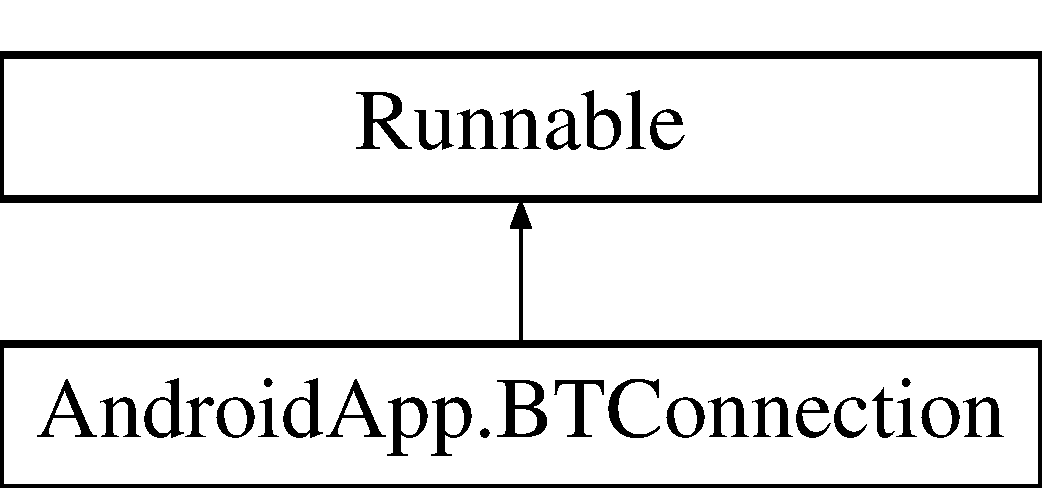
\includegraphics[height=2.000000cm]{class_android_app_1_1_b_t_connection}
\end{center}
\end{figure}
\subsection*{Public Member Functions}
\begin{DoxyCompactItemize}
\item 
\hyperlink{class_android_app_1_1_b_t_connection_a9211856a493caa2423f07e36c2fd12b6}{B\+T\+Connection} (Bluetooth\+Device \hyperlink{class_android_app_1_1_b_t_connection_a3ed1e51b0f24f0b20ca5c27270f2999c}{bt\+Device})  throws I\+O\+Exception 
\begin{DoxyCompactList}\small\item\em Constructor for \hyperlink{class_android_app_1_1_b_t_connection}{B\+T\+Connection} class. \end{DoxyCompactList}\item 
void \hyperlink{class_android_app_1_1_b_t_connection_a41022747db3c5a8bf0f4ddbc7bf32a3d}{set\+R\+X\+Handler} (Handler new\+Handler)
\begin{DoxyCompactList}\small\item\em Setter function for R\+X\+Handler. \end{DoxyCompactList}\item 
Handler \hyperlink{class_android_app_1_1_b_t_connection_a2d2a381cb7cb2bcab1db0c804e85a32d}{get\+R\+X\+Handler} ()
\begin{DoxyCompactList}\small\item\em Getter function for R\+X\+Handler. \end{DoxyCompactList}\item 
void \hyperlink{class_android_app_1_1_b_t_connection_a03907fd685748cb0da88a7f17d90885f}{run} ()
\begin{DoxyCompactList}\small\item\em Main run procedure for new Runnable thread created. \end{DoxyCompactList}\item 
\mbox{\Hypertarget{class_android_app_1_1_b_t_connection_a4f542434c59f541d47b68a0e225cfea9}\label{class_android_app_1_1_b_t_connection_a4f542434c59f541d47b68a0e225cfea9}} 
void \hyperlink{class_android_app_1_1_b_t_connection_a4f542434c59f541d47b68a0e225cfea9}{stop} ()
\begin{DoxyCompactList}\small\item\em Procedure to stop the bluetooth connection thread from running. \end{DoxyCompactList}\item 
boolean \hyperlink{class_android_app_1_1_b_t_connection_a88abb39350aef278f15e54be4d0d1df3}{is\+Running} ()
\begin{DoxyCompactList}\small\item\em Function to check whether main connection thread is running. \end{DoxyCompactList}\item 
boolean \hyperlink{class_android_app_1_1_b_t_connection_a1c91fcddfe9f3b69cd0141742103191a}{is\+Connected} ()
\begin{DoxyCompactList}\small\item\em Function to check whether BT connection is still valid. \end{DoxyCompactList}\end{DoxyCompactItemize}
\subsection*{Public Attributes}
\begin{DoxyCompactItemize}
\item 
final Handler \hyperlink{class_android_app_1_1_b_t_connection_a3236a74297d91f15dd63efc66f03a821}{tx\+Handler}
\begin{DoxyCompactList}\small\item\em Handler class for transmission of data. \end{DoxyCompactList}\end{DoxyCompactItemize}
\subsection*{Private Member Functions}
\begin{DoxyCompactItemize}
\item 
void \hyperlink{class_android_app_1_1_b_t_connection_a1dfc9451ba1b40089f17ee081486602e}{connect} ()  throws I\+O\+Exception 
\begin{DoxyCompactList}\small\item\em Procedure to create a connection to logging device. \end{DoxyCompactList}\item 
\mbox{\Hypertarget{class_android_app_1_1_b_t_connection_a37bb3e5c1dcf6b78a73239f6f62ab6d8}\label{class_android_app_1_1_b_t_connection_a37bb3e5c1dcf6b78a73239f6f62ab6d8}} 
void \hyperlink{class_android_app_1_1_b_t_connection_a37bb3e5c1dcf6b78a73239f6f62ab6d8}{close} ()  throws I\+O\+Exception 
\begin{DoxyCompactList}\small\item\em Closes the BT connection socket, exceptions thrown on failure. \end{DoxyCompactList}\end{DoxyCompactItemize}
\subsection*{Private Attributes}
\begin{DoxyCompactItemize}
\item 
\mbox{\Hypertarget{class_android_app_1_1_b_t_connection_a3ed1e51b0f24f0b20ca5c27270f2999c}\label{class_android_app_1_1_b_t_connection_a3ed1e51b0f24f0b20ca5c27270f2999c}} 
Bluetooth\+Device \hyperlink{class_android_app_1_1_b_t_connection_a3ed1e51b0f24f0b20ca5c27270f2999c}{bt\+Device}
\begin{DoxyCompactList}\small\item\em Bluetooth Device object, holds information for chosen slave. \end{DoxyCompactList}\item 
\mbox{\Hypertarget{class_android_app_1_1_b_t_connection_a4e3bfea96a4ddbd2cd2b76bb4ce8b871}\label{class_android_app_1_1_b_t_connection_a4e3bfea96a4ddbd2cd2b76bb4ce8b871}} 
Handler \hyperlink{class_android_app_1_1_b_t_connection_a4e3bfea96a4ddbd2cd2b76bb4ce8b871}{R\+X\+Handler} = null
\begin{DoxyCompactList}\small\item\em Handler function where received data is sent to. \end{DoxyCompactList}\item 
\mbox{\Hypertarget{class_android_app_1_1_b_t_connection_af3cdc6c880b28361d87d0118ace0e49c}\label{class_android_app_1_1_b_t_connection_af3cdc6c880b28361d87d0118ace0e49c}} 
Bluetooth\+Socket \hyperlink{class_android_app_1_1_b_t_connection_af3cdc6c880b28361d87d0118ace0e49c}{bt\+Socket} = null
\begin{DoxyCompactList}\small\item\em Socket created for bluetooth connection, used for T\+X/\+RX. \end{DoxyCompactList}\item 
\mbox{\Hypertarget{class_android_app_1_1_b_t_connection_ace01a7a97f5d1abccb61a5d6c6ad9295}\label{class_android_app_1_1_b_t_connection_ace01a7a97f5d1abccb61a5d6c6ad9295}} 
volatile boolean \hyperlink{class_android_app_1_1_b_t_connection_ace01a7a97f5d1abccb61a5d6c6ad9295}{running} = false
\begin{DoxyCompactList}\small\item\em Indicates whether main run thread is in progress. \end{DoxyCompactList}\end{DoxyCompactItemize}
\subsection*{Static Private Attributes}
\begin{DoxyCompactItemize}
\item 
\mbox{\Hypertarget{class_android_app_1_1_b_t_connection_ad838024d59c68be866b5db329d6f6230}\label{class_android_app_1_1_b_t_connection_ad838024d59c68be866b5db329d6f6230}} 
static final String \hyperlink{class_android_app_1_1_b_t_connection_ad838024d59c68be866b5db329d6f6230}{T\+AG} = \char`\"{}B\+T\+Connection\char`\"{}
\begin{DoxyCompactList}\small\item\em Tag using for debugging. \end{DoxyCompactList}\item 
\mbox{\Hypertarget{class_android_app_1_1_b_t_connection_a0e531d4cad0e5cca1e5b4446551b5c63}\label{class_android_app_1_1_b_t_connection_a0e531d4cad0e5cca1e5b4446551b5c63}} 
static final U\+U\+ID \hyperlink{class_android_app_1_1_b_t_connection_a0e531d4cad0e5cca1e5b4446551b5c63}{uuid} = U\+U\+I\+D.\+from\+String(\char`\"{}00001101-\/0000-\/1000-\/8000-\/00805f9b34fb\char`\"{})
\begin{DoxyCompactList}\small\item\em U\+U\+ID to allow Serial connection via BT. \end{DoxyCompactList}\item 
\mbox{\Hypertarget{class_android_app_1_1_b_t_connection_afe2f59edec0610e765222e02ab350e84}\label{class_android_app_1_1_b_t_connection_afe2f59edec0610e765222e02ab350e84}} 
static final String \hyperlink{class_android_app_1_1_b_t_connection_afe2f59edec0610e765222e02ab350e84}{N\+E\+W\+\_\+\+L\+I\+NE} = \char`\"{}\textbackslash{}r\textbackslash{}n\char`\"{}
\begin{DoxyCompactList}\small\item\em New line string. \end{DoxyCompactList}\end{DoxyCompactItemize}


\subsection{Detailed Description}
Thread class for a new bluetooth connection to a device. 

\subsection{Constructor \& Destructor Documentation}
\mbox{\Hypertarget{class_android_app_1_1_b_t_connection_a9211856a493caa2423f07e36c2fd12b6}\label{class_android_app_1_1_b_t_connection_a9211856a493caa2423f07e36c2fd12b6}} 
\index{Android\+App\+::\+B\+T\+Connection@{Android\+App\+::\+B\+T\+Connection}!B\+T\+Connection@{B\+T\+Connection}}
\index{B\+T\+Connection@{B\+T\+Connection}!Android\+App\+::\+B\+T\+Connection@{Android\+App\+::\+B\+T\+Connection}}
\subsubsection{\texorpdfstring{B\+T\+Connection()}{BTConnection()}}
{\footnotesize\ttfamily Android\+App.\+B\+T\+Connection.\+B\+T\+Connection (\begin{DoxyParamCaption}\item[{Bluetooth\+Device}]{bt\+Device }\end{DoxyParamCaption}) throws I\+O\+Exception\hspace{0.3cm}{\ttfamily [inline]}}



Constructor for \hyperlink{class_android_app_1_1_b_t_connection}{B\+T\+Connection} class. 

Sets the BT device interface used for this class and attempts a connection.


\begin{DoxyParams}{Parameters}
{\em bt\+Device} & -\/ Device used for creating connection. \\
\hline
\end{DoxyParams}

\begin{DoxyCode}
59                                \{
60         this.\hyperlink{class_android_app_1_1_b_t_connection_a3ed1e51b0f24f0b20ca5c27270f2999c}{btDevice} = \hyperlink{class_android_app_1_1_b_t_connection_a3ed1e51b0f24f0b20ca5c27270f2999c}{btDevice};
61 
62         \textcolor{comment}{/* Connect the device so ready to use run */}
63         \hyperlink{class_android_app_1_1_b_t_connection_a1dfc9451ba1b40089f17ee081486602e}{connect}();
64     \}
\end{DoxyCode}


\subsection{Member Function Documentation}
\mbox{\Hypertarget{class_android_app_1_1_b_t_connection_a41022747db3c5a8bf0f4ddbc7bf32a3d}\label{class_android_app_1_1_b_t_connection_a41022747db3c5a8bf0f4ddbc7bf32a3d}} 
\index{Android\+App\+::\+B\+T\+Connection@{Android\+App\+::\+B\+T\+Connection}!set\+R\+X\+Handler@{set\+R\+X\+Handler}}
\index{set\+R\+X\+Handler@{set\+R\+X\+Handler}!Android\+App\+::\+B\+T\+Connection@{Android\+App\+::\+B\+T\+Connection}}
\subsubsection{\texorpdfstring{set\+R\+X\+Handler()}{setRXHandler()}}
{\footnotesize\ttfamily void Android\+App.\+B\+T\+Connection.\+set\+R\+X\+Handler (\begin{DoxyParamCaption}\item[{Handler}]{new\+Handler }\end{DoxyParamCaption})\hspace{0.3cm}{\ttfamily [inline]}}



Setter function for R\+X\+Handler. 


\begin{DoxyParams}{Parameters}
{\em new\+Handler} & -\/ The new Handler where RX\textquotesingle{}d data will be sent to. \\
\hline
\end{DoxyParams}

\begin{DoxyCode}
108                                                  \{
109         \hyperlink{class_android_app_1_1_b_t_connection_a4e3bfea96a4ddbd2cd2b76bb4ce8b871}{RXHandler} = newHandler;
110     \}
\end{DoxyCode}
\mbox{\Hypertarget{class_android_app_1_1_b_t_connection_a2d2a381cb7cb2bcab1db0c804e85a32d}\label{class_android_app_1_1_b_t_connection_a2d2a381cb7cb2bcab1db0c804e85a32d}} 
\index{Android\+App\+::\+B\+T\+Connection@{Android\+App\+::\+B\+T\+Connection}!get\+R\+X\+Handler@{get\+R\+X\+Handler}}
\index{get\+R\+X\+Handler@{get\+R\+X\+Handler}!Android\+App\+::\+B\+T\+Connection@{Android\+App\+::\+B\+T\+Connection}}
\subsubsection{\texorpdfstring{get\+R\+X\+Handler()}{getRXHandler()}}
{\footnotesize\ttfamily Handler Android\+App.\+B\+T\+Connection.\+get\+R\+X\+Handler (\begin{DoxyParamCaption}{ }\end{DoxyParamCaption})\hspace{0.3cm}{\ttfamily [inline]}}



Getter function for R\+X\+Handler. 

\begin{DoxyReturn}{Returns}
Handler -\/ The RX handler for BT connection. 
\end{DoxyReturn}

\begin{DoxyCode}
117                                   \{
118         \textcolor{keywordflow}{return} \hyperlink{class_android_app_1_1_b_t_connection_a4e3bfea96a4ddbd2cd2b76bb4ce8b871}{RXHandler};
119     \}
\end{DoxyCode}
\mbox{\Hypertarget{class_android_app_1_1_b_t_connection_a03907fd685748cb0da88a7f17d90885f}\label{class_android_app_1_1_b_t_connection_a03907fd685748cb0da88a7f17d90885f}} 
\index{Android\+App\+::\+B\+T\+Connection@{Android\+App\+::\+B\+T\+Connection}!run@{run}}
\index{run@{run}!Android\+App\+::\+B\+T\+Connection@{Android\+App\+::\+B\+T\+Connection}}
\subsubsection{\texorpdfstring{run()}{run()}}
{\footnotesize\ttfamily void Android\+App.\+B\+T\+Connection.\+run (\begin{DoxyParamCaption}{ }\end{DoxyParamCaption})\hspace{0.3cm}{\ttfamily [inline]}}



Main run procedure for new Runnable thread created. 

If connected procedure waits for data to be received. Parsing this received into lines and then splitting each line into a J\+S\+O\+N\+Object. If a valid J\+S\+O\+N\+Object is found it is then sends to the receive handler in a seperate thread (using messages). 
\begin{DoxyCode}
130                       \{
131         InputStream RXStream;
132 
133         \textcolor{comment}{/* Indicate that we are now running main thread */}
134         \hyperlink{class_android_app_1_1_b_t_connection_ace01a7a97f5d1abccb61a5d6c6ad9295}{running} = \textcolor{keyword}{true};
135 
136         \textcolor{keywordflow}{if} (\hyperlink{class_android_app_1_1_b_t_connection_a1c91fcddfe9f3b69cd0141742103191a}{isConnected}()) \{
137             \textcolor{comment}{/* Get our input stream for receiving bytes */}
138             \textcolor{keywordflow}{try} \{
139                 RXStream = \hyperlink{class_android_app_1_1_b_t_connection_af3cdc6c880b28361d87d0118ace0e49c}{btSocket}.getInputStream();
140             \} \textcolor{keywordflow}{catch} (IOException e) \{
141                 Log.e(\hyperlink{class_android_app_1_1_b_t_connection_ad838024d59c68be866b5db329d6f6230}{TAG}, \textcolor{stringliteral}{"Unable to get RXStream"}, e);
142                 \hyperlink{class_android_app_1_1_b_t_connection_ace01a7a97f5d1abccb61a5d6c6ad9295}{running} = \textcolor{keyword}{false};
143                 \textcolor{keywordflow}{return};
144             \}
145 
146             \textcolor{comment}{/*}
147 \textcolor{comment}{             * While still connected and not signalled to stop we receive data}
148 \textcolor{comment}{             * and then send it to the handler}
149 \textcolor{comment}{             */}
150             String recvBuff = \textcolor{stringliteral}{""};
151             \textcolor{keywordflow}{while} (\hyperlink{class_android_app_1_1_b_t_connection_a88abb39350aef278f15e54be4d0d1df3}{isRunning}() && \hyperlink{class_android_app_1_1_b_t_connection_a1c91fcddfe9f3b69cd0141742103191a}{isConnected}()) \{
152                 \textcolor{keywordflow}{try} \{
153                     \textcolor{keywordtype}{int} bytesAvailable = RXStream.available();
154 
155                     \textcolor{keywordflow}{if} (bytesAvailable > 0) \{
156                         byte[] packetBytes = \textcolor{keyword}{new} byte[bytesAvailable];
157                         \textcolor{keywordtype}{int} bytesRead = RXStream.read(packetBytes, 0, bytesAvailable);
158 
159                         recvBuff += \textcolor{keyword}{new} String(packetBytes);
160                     \}
161 
162                     \textcolor{keywordflow}{if} (\hyperlink{class_android_app_1_1_b_t_connection_a4e3bfea96a4ddbd2cd2b76bb4ce8b871}{RXHandler} != null) \{
163 
164                         \textcolor{keywordflow}{if} (recvBuff.indexOf(\hyperlink{class_android_app_1_1_b_t_connection_afe2f59edec0610e765222e02ab350e84}{NEW\_LINE}) > 0) \{
165 
166                             String jsonLine = recvBuff.substring(0, recvBuff.indexOf(
      \hyperlink{class_android_app_1_1_b_t_connection_afe2f59edec0610e765222e02ab350e84}{NEW\_LINE}));
167 
168                             \textcolor{comment}{/*}
169 \textcolor{comment}{                             * Having to send data to main thread using messages}
170 \textcolor{comment}{                             * as we are multithreading.}
171 \textcolor{comment}{                             * If we try and use a standard call to function}
172 \textcolor{comment}{                             * will cause a crash.}
173 \textcolor{comment}{                             */}
174                             Bundle dataBundle =  \textcolor{keyword}{new} Bundle();
175                             dataBundle.putString(\textcolor{stringliteral}{"JSON"}, jsonLine);
176 
177                             Message message = \hyperlink{class_android_app_1_1_b_t_connection_a4e3bfea96a4ddbd2cd2b76bb4ce8b871}{RXHandler}.obtainMessage();
178                             message.setData(dataBundle);
179                             message.sendToTarget();
180 
181                             recvBuff = recvBuff.replace(jsonLine + \hyperlink{class_android_app_1_1_b_t_connection_afe2f59edec0610e765222e02ab350e84}{NEW\_LINE}, \textcolor{stringliteral}{""});
182                         \}
183                     \}
184 
185                 \} \textcolor{keywordflow}{catch} (IOException e) \{
186                     Log.e(\hyperlink{class_android_app_1_1_b_t_connection_ad838024d59c68be866b5db329d6f6230}{TAG}, \textcolor{stringliteral}{"Unable to read data"}, e);
187                     \hyperlink{class_android_app_1_1_b_t_connection_ace01a7a97f5d1abccb61a5d6c6ad9295}{running} = \textcolor{keyword}{false};
188                     \textcolor{keywordflow}{return};
189                 \}
190             \}
191 
192         \}
193 
194         \textcolor{comment}{/* Close bluetooth socket */}
195         \textcolor{keywordflow}{try} \{
196             this.\hyperlink{class_android_app_1_1_b_t_connection_a37bb3e5c1dcf6b78a73239f6f62ab6d8}{close}();
197         \} \textcolor{keywordflow}{catch} (IOException e) \{
198             \textcolor{comment}{/* Do nothing */}
199         \}
200 
201         \textcolor{comment}{/* Null BT socket to show needs to reconnect */}
202         \hyperlink{class_android_app_1_1_b_t_connection_af3cdc6c880b28361d87d0118ace0e49c}{btSocket} = null;
203         \hyperlink{class_android_app_1_1_b_t_connection_ace01a7a97f5d1abccb61a5d6c6ad9295}{running} = \textcolor{keyword}{false};
204     \}
\end{DoxyCode}
\mbox{\Hypertarget{class_android_app_1_1_b_t_connection_a88abb39350aef278f15e54be4d0d1df3}\label{class_android_app_1_1_b_t_connection_a88abb39350aef278f15e54be4d0d1df3}} 
\index{Android\+App\+::\+B\+T\+Connection@{Android\+App\+::\+B\+T\+Connection}!is\+Running@{is\+Running}}
\index{is\+Running@{is\+Running}!Android\+App\+::\+B\+T\+Connection@{Android\+App\+::\+B\+T\+Connection}}
\subsubsection{\texorpdfstring{is\+Running()}{isRunning()}}
{\footnotesize\ttfamily boolean Android\+App.\+B\+T\+Connection.\+is\+Running (\begin{DoxyParamCaption}{ }\end{DoxyParamCaption})\hspace{0.3cm}{\ttfamily [inline]}}



Function to check whether main connection thread is running. 

\begin{DoxyReturn}{Returns}
boolean -\/ Whether thread is running. 
\end{DoxyReturn}

\begin{DoxyCode}
217                                \{
218         \textcolor{keywordflow}{return} \hyperlink{class_android_app_1_1_b_t_connection_ace01a7a97f5d1abccb61a5d6c6ad9295}{running};
219     \}
\end{DoxyCode}
\mbox{\Hypertarget{class_android_app_1_1_b_t_connection_a1c91fcddfe9f3b69cd0141742103191a}\label{class_android_app_1_1_b_t_connection_a1c91fcddfe9f3b69cd0141742103191a}} 
\index{Android\+App\+::\+B\+T\+Connection@{Android\+App\+::\+B\+T\+Connection}!is\+Connected@{is\+Connected}}
\index{is\+Connected@{is\+Connected}!Android\+App\+::\+B\+T\+Connection@{Android\+App\+::\+B\+T\+Connection}}
\subsubsection{\texorpdfstring{is\+Connected()}{isConnected()}}
{\footnotesize\ttfamily boolean Android\+App.\+B\+T\+Connection.\+is\+Connected (\begin{DoxyParamCaption}{ }\end{DoxyParamCaption})\hspace{0.3cm}{\ttfamily [inline]}}



Function to check whether BT connection is still valid. 

\begin{DoxyReturn}{Returns}
boolean -\/ Whether connection is still available. 
\end{DoxyReturn}

\begin{DoxyCode}
225                                  \{
226         \textcolor{keywordtype}{boolean} result = \textcolor{keyword}{false};
227 
228         \textcolor{keywordflow}{if} (\hyperlink{class_android_app_1_1_b_t_connection_af3cdc6c880b28361d87d0118ace0e49c}{btSocket} != null) \{
229             \textcolor{keywordflow}{if} (\hyperlink{class_android_app_1_1_b_t_connection_af3cdc6c880b28361d87d0118ace0e49c}{btSocket}.isConnected())
230                 result = \textcolor{keyword}{true};
231         \}
232         \textcolor{keywordflow}{return} result;
233     \}
\end{DoxyCode}
\mbox{\Hypertarget{class_android_app_1_1_b_t_connection_a1dfc9451ba1b40089f17ee081486602e}\label{class_android_app_1_1_b_t_connection_a1dfc9451ba1b40089f17ee081486602e}} 
\index{Android\+App\+::\+B\+T\+Connection@{Android\+App\+::\+B\+T\+Connection}!connect@{connect}}
\index{connect@{connect}!Android\+App\+::\+B\+T\+Connection@{Android\+App\+::\+B\+T\+Connection}}
\subsubsection{\texorpdfstring{connect()}{connect()}}
{\footnotesize\ttfamily void Android\+App.\+B\+T\+Connection.\+connect (\begin{DoxyParamCaption}{ }\end{DoxyParamCaption}) throws I\+O\+Exception\hspace{0.3cm}{\ttfamily [inline]}, {\ttfamily [private]}}



Procedure to create a connection to logging device. 

Creates a raw Serial socket via U\+U\+ID and then attempts to connect. Exceptions thrown on failure. 
\begin{DoxyCode}
241                                               \{
242 
243         \textcolor{comment}{/* Attempt to make connection to remote device, throw exception if not */}
244         \textcolor{keywordflow}{try} \{
245             \hyperlink{class_android_app_1_1_b_t_connection_af3cdc6c880b28361d87d0118ace0e49c}{btSocket} = \hyperlink{class_android_app_1_1_b_t_connection_a3ed1e51b0f24f0b20ca5c27270f2999c}{btDevice}.createRfcommSocketToServiceRecord(
      \hyperlink{class_android_app_1_1_b_t_connection_a0e531d4cad0e5cca1e5b4446551b5c63}{uuid});
246         \} \textcolor{keywordflow}{catch} (IOException e) \{
247             Log.e(\hyperlink{class_android_app_1_1_b_t_connection_ad838024d59c68be866b5db329d6f6230}{TAG}, \textcolor{stringliteral}{"Unable to create RFCOMM"}, e);
248             \textcolor{keywordflow}{throw} e;
249         \}
250 
251         \textcolor{keywordflow}{try} \{
252             \hyperlink{class_android_app_1_1_b_t_connection_af3cdc6c880b28361d87d0118ace0e49c}{btSocket}.connect();
253         \} \textcolor{keywordflow}{catch} (IOException e) \{
254             Log.e(\hyperlink{class_android_app_1_1_b_t_connection_ad838024d59c68be866b5db329d6f6230}{TAG}, \textcolor{stringliteral}{"Unable to connect"}, e);
255 
256             \textcolor{comment}{/* Close our socket as unable to connect */}
257             \textcolor{keywordflow}{try} \{
258                 this.\hyperlink{class_android_app_1_1_b_t_connection_a37bb3e5c1dcf6b78a73239f6f62ab6d8}{close}();
259             \} \textcolor{keywordflow}{catch} (IOException e2) \{
260                 \textcolor{keywordflow}{throw} e2;
261             \}
262             \textcolor{keywordflow}{throw} e;
263         \}
264     \}
\end{DoxyCode}


\subsection{Member Data Documentation}
\mbox{\Hypertarget{class_android_app_1_1_b_t_connection_a3236a74297d91f15dd63efc66f03a821}\label{class_android_app_1_1_b_t_connection_a3236a74297d91f15dd63efc66f03a821}} 
\index{Android\+App\+::\+B\+T\+Connection@{Android\+App\+::\+B\+T\+Connection}!tx\+Handler@{tx\+Handler}}
\index{tx\+Handler@{tx\+Handler}!Android\+App\+::\+B\+T\+Connection@{Android\+App\+::\+B\+T\+Connection}}
\subsubsection{\texorpdfstring{tx\+Handler}{txHandler}}
{\footnotesize\ttfamily final Handler Android\+App.\+B\+T\+Connection.\+tx\+Handler}

{\bfseries Initial value\+:}
\begin{DoxyCode}
= \textcolor{keyword}{new} Handler(Looper.getMainLooper()) \{

        
        @Override
        \textcolor{keyword}{public} \textcolor{keywordtype}{void} handleMessage(Message msg) \{

            
            \textcolor{keywordflow}{if} (\hyperlink{class_android_app_1_1_b_t_connection_a1c91fcddfe9f3b69cd0141742103191a}{isConnected}() && \hyperlink{class_android_app_1_1_b_t_connection_a88abb39350aef278f15e54be4d0d1df3}{isRunning}()) \{
                OutputStream TXStream;

                
                \textcolor{keywordflow}{try} \{
                    TXStream = \hyperlink{class_android_app_1_1_b_t_connection_af3cdc6c880b28361d87d0118ace0e49c}{btSocket}.getOutputStream();

                    String txString = (String)msg.obj;
                    TXStream.write(txString.getBytes());
                \} \textcolor{keywordflow}{catch} (IOException e) \{
                    Log.e(\hyperlink{class_android_app_1_1_b_t_connection_ad838024d59c68be866b5db329d6f6230}{TAG}, \textcolor{stringliteral}{"Unable to use TXStream"}, e);
                    \textcolor{keywordflow}{return};
                \}
            \}
        \}
    \}
\end{DoxyCode}


Handler class for transmission of data. 

Messages containing data to be transmitted are sent from main UI thread. 

The documentation for this class was generated from the following file\+:\begin{DoxyCompactItemize}
\item 
android-\/app/app/src/main/java/com/jack/motorbikestatistics/\hyperlink{_b_t_connection_8java}{B\+T\+Connection.\+java}\end{DoxyCompactItemize}

\hypertarget{class_android_app_1_1_b_t_device_item}{}\section{Android\+App.\+B\+T\+Device\+Item Class Reference}
\label{class_android_app_1_1_b_t_device_item}\index{Android\+App.\+B\+T\+Device\+Item@{Android\+App.\+B\+T\+Device\+Item}}


Class used for holding core UI information of a bluetooth devices.  


\subsection*{Public Member Functions}
\begin{DoxyCompactItemize}
\item 
\hyperlink{class_android_app_1_1_b_t_connection}{B\+T\+Connection} \hyperlink{class_android_app_1_1_b_t_device_item_af256e53bf23dd3f969b14e0566a7b785}{get\+Connection} ()
\begin{DoxyCompactList}\small\item\em Getter for the bluetooth connection of specified device. \end{DoxyCompactList}\item 
void \hyperlink{class_android_app_1_1_b_t_device_item_a7fa3ffc652503e2a767e6cfb74a2fe55}{set\+Connection} (\hyperlink{class_android_app_1_1_b_t_connection}{B\+T\+Connection} new\+Conn)
\begin{DoxyCompactList}\small\item\em Setter for setting the Device\+Item object\textquotesingle{}s connection. \end{DoxyCompactList}\item 
Bluetooth\+Device \hyperlink{class_android_app_1_1_b_t_device_item_a2e8577754ccc57fb1d9e94f818d41151}{get\+Device} ()
\begin{DoxyCompactList}\small\item\em Getter for BT device object (contains name, H\+W\+ID etc.). \end{DoxyCompactList}\item 
String \hyperlink{class_android_app_1_1_b_t_device_item_a5a27acd244054ade34a6acd4a311e028}{get\+Status} ()
\begin{DoxyCompactList}\small\item\em Getter for current status of \hyperlink{class_android_app_1_1_b_t_device_item}{B\+T\+Device\+Item}. \end{DoxyCompactList}\item 
void \hyperlink{class_android_app_1_1_b_t_device_item_a3e7e6d991363b670a71f4634bc5e4f27}{set\+Status} (String new\+Status)
\begin{DoxyCompactList}\small\item\em Setter for current status of \hyperlink{class_android_app_1_1_b_t_device_item}{B\+T\+Device\+Item}. \end{DoxyCompactList}\item 
int \hyperlink{class_android_app_1_1_b_t_device_item_a42c00ce200fd487f51e2016ed65cdf22}{get\+Icon\+ID} ()
\begin{DoxyCompactList}\small\item\em Getter for icon ID to use in List\+View. \end{DoxyCompactList}\item 
void \hyperlink{class_android_app_1_1_b_t_device_item_a893140b78c17184a199ac419f0fc7be7}{set\+Icon\+ID} (int new\+ID)
\begin{DoxyCompactList}\small\item\em Setter for icon ID to use in List\+View. \end{DoxyCompactList}\item 
\hyperlink{class_android_app_1_1_b_t_device_item_a8a172bb68f01d765ec832d62008502bc}{B\+T\+Device\+Item} (Bluetooth\+Device \hyperlink{class_android_app_1_1_b_t_device_item_a3f62f8de1d815f2e4f59030565ba29a1}{device}, String \hyperlink{class_android_app_1_1_b_t_device_item_a53c37efab7ea4550d4db428b3d6915e0}{status}, int \hyperlink{class_android_app_1_1_b_t_device_item_aa008dfacbd2f948952a14bed413d5969}{icon\+ID})
\begin{DoxyCompactList}\small\item\em Constructor for \hyperlink{class_android_app_1_1_b_t_device_item}{B\+T\+Device\+Item} class. \end{DoxyCompactList}\end{DoxyCompactItemize}
\subsection*{Private Attributes}
\begin{DoxyCompactItemize}
\item 
\mbox{\Hypertarget{class_android_app_1_1_b_t_device_item_a9a95ded58a8607664d020946e4e38364}\label{class_android_app_1_1_b_t_device_item_a9a95ded58a8607664d020946e4e38364}} 
\hyperlink{class_android_app_1_1_b_t_connection}{B\+T\+Connection} \hyperlink{class_android_app_1_1_b_t_device_item_a9a95ded58a8607664d020946e4e38364}{connection} = null
\begin{DoxyCompactList}\small\item\em Variable for \hyperlink{class_android_app_1_1_b_t_connection}{B\+T\+Connection} if device is already connected. \end{DoxyCompactList}\item 
\mbox{\Hypertarget{class_android_app_1_1_b_t_device_item_aa008dfacbd2f948952a14bed413d5969}\label{class_android_app_1_1_b_t_device_item_aa008dfacbd2f948952a14bed413d5969}} 
int \hyperlink{class_android_app_1_1_b_t_device_item_aa008dfacbd2f948952a14bed413d5969}{icon\+ID}
\begin{DoxyCompactList}\small\item\em ID of icon to use within the List\+View. \end{DoxyCompactList}\item 
\mbox{\Hypertarget{class_android_app_1_1_b_t_device_item_a3f62f8de1d815f2e4f59030565ba29a1}\label{class_android_app_1_1_b_t_device_item_a3f62f8de1d815f2e4f59030565ba29a1}} 
Bluetooth\+Device \hyperlink{class_android_app_1_1_b_t_device_item_a3f62f8de1d815f2e4f59030565ba29a1}{device}
\begin{DoxyCompactList}\small\item\em Device object that holds info such as name, H\+W\+ID etc. \end{DoxyCompactList}\item 
\mbox{\Hypertarget{class_android_app_1_1_b_t_device_item_a53c37efab7ea4550d4db428b3d6915e0}\label{class_android_app_1_1_b_t_device_item_a53c37efab7ea4550d4db428b3d6915e0}} 
String \hyperlink{class_android_app_1_1_b_t_device_item_a53c37efab7ea4550d4db428b3d6915e0}{status}
\begin{DoxyCompactList}\small\item\em Status of the device, unpaired, paired, connected. \end{DoxyCompactList}\end{DoxyCompactItemize}


\subsection{Detailed Description}
Class used for holding core UI information of a bluetooth devices. 

\subsection{Constructor \& Destructor Documentation}
\mbox{\Hypertarget{class_android_app_1_1_b_t_device_item_a8a172bb68f01d765ec832d62008502bc}\label{class_android_app_1_1_b_t_device_item_a8a172bb68f01d765ec832d62008502bc}} 
\index{Android\+App\+::\+B\+T\+Device\+Item@{Android\+App\+::\+B\+T\+Device\+Item}!B\+T\+Device\+Item@{B\+T\+Device\+Item}}
\index{B\+T\+Device\+Item@{B\+T\+Device\+Item}!Android\+App\+::\+B\+T\+Device\+Item@{Android\+App\+::\+B\+T\+Device\+Item}}
\subsubsection{\texorpdfstring{B\+T\+Device\+Item()}{BTDeviceItem()}}
{\footnotesize\ttfamily Android\+App.\+B\+T\+Device\+Item.\+B\+T\+Device\+Item (\begin{DoxyParamCaption}\item[{Bluetooth\+Device}]{device,  }\item[{String}]{status,  }\item[{int}]{icon\+ID }\end{DoxyParamCaption})\hspace{0.3cm}{\ttfamily [inline]}}



Constructor for \hyperlink{class_android_app_1_1_b_t_device_item}{B\+T\+Device\+Item} class. 

Called when new Bluetooth\+Device is found during discovery, so that it can be added to the device List\+View.


\begin{DoxyParams}{Parameters}
{\em device} & -\/ Bluetooth\+Device containing H\+W\+ID, name, etc. \\
\hline
{\em status} & -\/ Current status of the discovered device. \\
\hline
{\em icon\+ID} & -\/ Icon ID to display within the List\+View. \\
\hline
\end{DoxyParams}

\begin{DoxyCode}
96     \{
97         this.\hyperlink{class_android_app_1_1_b_t_device_item_a3f62f8de1d815f2e4f59030565ba29a1}{device} = \hyperlink{class_android_app_1_1_b_t_device_item_a3f62f8de1d815f2e4f59030565ba29a1}{device};
98         this.\hyperlink{class_android_app_1_1_b_t_device_item_a53c37efab7ea4550d4db428b3d6915e0}{status} = \hyperlink{class_android_app_1_1_b_t_device_item_a53c37efab7ea4550d4db428b3d6915e0}{status};
99         this.\hyperlink{class_android_app_1_1_b_t_device_item_aa008dfacbd2f948952a14bed413d5969}{iconID} = \hyperlink{class_android_app_1_1_b_t_device_item_aa008dfacbd2f948952a14bed413d5969}{iconID};
100     \}
\end{DoxyCode}


\subsection{Member Function Documentation}
\mbox{\Hypertarget{class_android_app_1_1_b_t_device_item_af256e53bf23dd3f969b14e0566a7b785}\label{class_android_app_1_1_b_t_device_item_af256e53bf23dd3f969b14e0566a7b785}} 
\index{Android\+App\+::\+B\+T\+Device\+Item@{Android\+App\+::\+B\+T\+Device\+Item}!get\+Connection@{get\+Connection}}
\index{get\+Connection@{get\+Connection}!Android\+App\+::\+B\+T\+Device\+Item@{Android\+App\+::\+B\+T\+Device\+Item}}
\subsubsection{\texorpdfstring{get\+Connection()}{getConnection()}}
{\footnotesize\ttfamily \hyperlink{class_android_app_1_1_b_t_connection}{B\+T\+Connection} Android\+App.\+B\+T\+Device\+Item.\+get\+Connection (\begin{DoxyParamCaption}{ }\end{DoxyParamCaption})\hspace{0.3cm}{\ttfamily [inline]}}



Getter for the bluetooth connection of specified device. 

\begin{DoxyReturn}{Returns}
\hyperlink{class_android_app_1_1_b_t_connection}{B\+T\+Connection} -\/ Connection between app \& logging device. 
\end{DoxyReturn}

\begin{DoxyCode}
33                                         \{
34         \textcolor{keywordflow}{return} \hyperlink{class_android_app_1_1_b_t_device_item_a9a95ded58a8607664d020946e4e38364}{connection};
35     \}
\end{DoxyCode}
\mbox{\Hypertarget{class_android_app_1_1_b_t_device_item_a7fa3ffc652503e2a767e6cfb74a2fe55}\label{class_android_app_1_1_b_t_device_item_a7fa3ffc652503e2a767e6cfb74a2fe55}} 
\index{Android\+App\+::\+B\+T\+Device\+Item@{Android\+App\+::\+B\+T\+Device\+Item}!set\+Connection@{set\+Connection}}
\index{set\+Connection@{set\+Connection}!Android\+App\+::\+B\+T\+Device\+Item@{Android\+App\+::\+B\+T\+Device\+Item}}
\subsubsection{\texorpdfstring{set\+Connection()}{setConnection()}}
{\footnotesize\ttfamily void Android\+App.\+B\+T\+Device\+Item.\+set\+Connection (\begin{DoxyParamCaption}\item[{\hyperlink{class_android_app_1_1_b_t_connection}{B\+T\+Connection}}]{new\+Conn }\end{DoxyParamCaption})\hspace{0.3cm}{\ttfamily [inline]}}



Setter for setting the Device\+Item object\textquotesingle{}s connection. 


\begin{DoxyParams}{Parameters}
{\em new\+Conn} & -\/ New connection between app \& logging device. \\
\hline
\end{DoxyParams}

\begin{DoxyCode}
41                                                     \{
42         \hyperlink{class_android_app_1_1_b_t_device_item_a9a95ded58a8607664d020946e4e38364}{connection} = newConn;
43     \}
\end{DoxyCode}
\mbox{\Hypertarget{class_android_app_1_1_b_t_device_item_a2e8577754ccc57fb1d9e94f818d41151}\label{class_android_app_1_1_b_t_device_item_a2e8577754ccc57fb1d9e94f818d41151}} 
\index{Android\+App\+::\+B\+T\+Device\+Item@{Android\+App\+::\+B\+T\+Device\+Item}!get\+Device@{get\+Device}}
\index{get\+Device@{get\+Device}!Android\+App\+::\+B\+T\+Device\+Item@{Android\+App\+::\+B\+T\+Device\+Item}}
\subsubsection{\texorpdfstring{get\+Device()}{getDevice()}}
{\footnotesize\ttfamily Bluetooth\+Device Android\+App.\+B\+T\+Device\+Item.\+get\+Device (\begin{DoxyParamCaption}{ }\end{DoxyParamCaption})\hspace{0.3cm}{\ttfamily [inline]}}



Getter for BT device object (contains name, H\+W\+ID etc.). 

\begin{DoxyReturn}{Returns}
Bluetooth\+Device -\/ The bluetooth device object. 
\end{DoxyReturn}

\begin{DoxyCode}
49                                        \{
50         \textcolor{keywordflow}{return} \hyperlink{class_android_app_1_1_b_t_device_item_a3f62f8de1d815f2e4f59030565ba29a1}{device};
51     \}
\end{DoxyCode}
\mbox{\Hypertarget{class_android_app_1_1_b_t_device_item_a5a27acd244054ade34a6acd4a311e028}\label{class_android_app_1_1_b_t_device_item_a5a27acd244054ade34a6acd4a311e028}} 
\index{Android\+App\+::\+B\+T\+Device\+Item@{Android\+App\+::\+B\+T\+Device\+Item}!get\+Status@{get\+Status}}
\index{get\+Status@{get\+Status}!Android\+App\+::\+B\+T\+Device\+Item@{Android\+App\+::\+B\+T\+Device\+Item}}
\subsubsection{\texorpdfstring{get\+Status()}{getStatus()}}
{\footnotesize\ttfamily String Android\+App.\+B\+T\+Device\+Item.\+get\+Status (\begin{DoxyParamCaption}{ }\end{DoxyParamCaption})\hspace{0.3cm}{\ttfamily [inline]}}



Getter for current status of \hyperlink{class_android_app_1_1_b_t_device_item}{B\+T\+Device\+Item}. 

\begin{DoxyReturn}{Returns}
String -\/ Current status\+: unpaired, paired or connected. 
\end{DoxyReturn}

\begin{DoxyCode}
57                               \{
58         \textcolor{keywordflow}{return} \hyperlink{class_android_app_1_1_b_t_device_item_a53c37efab7ea4550d4db428b3d6915e0}{status};
59     \}
\end{DoxyCode}
\mbox{\Hypertarget{class_android_app_1_1_b_t_device_item_a3e7e6d991363b670a71f4634bc5e4f27}\label{class_android_app_1_1_b_t_device_item_a3e7e6d991363b670a71f4634bc5e4f27}} 
\index{Android\+App\+::\+B\+T\+Device\+Item@{Android\+App\+::\+B\+T\+Device\+Item}!set\+Status@{set\+Status}}
\index{set\+Status@{set\+Status}!Android\+App\+::\+B\+T\+Device\+Item@{Android\+App\+::\+B\+T\+Device\+Item}}
\subsubsection{\texorpdfstring{set\+Status()}{setStatus()}}
{\footnotesize\ttfamily void Android\+App.\+B\+T\+Device\+Item.\+set\+Status (\begin{DoxyParamCaption}\item[{String}]{new\+Status }\end{DoxyParamCaption})\hspace{0.3cm}{\ttfamily [inline]}}



Setter for current status of \hyperlink{class_android_app_1_1_b_t_device_item}{B\+T\+Device\+Item}. 


\begin{DoxyParams}{Parameters}
{\em new\+Status} & -\/ New string for status. \\
\hline
\end{DoxyParams}

\begin{DoxyCode}
65                                             \{
66         \hyperlink{class_android_app_1_1_b_t_device_item_a53c37efab7ea4550d4db428b3d6915e0}{status} = newStatus;
67     \}
\end{DoxyCode}
\mbox{\Hypertarget{class_android_app_1_1_b_t_device_item_a42c00ce200fd487f51e2016ed65cdf22}\label{class_android_app_1_1_b_t_device_item_a42c00ce200fd487f51e2016ed65cdf22}} 
\index{Android\+App\+::\+B\+T\+Device\+Item@{Android\+App\+::\+B\+T\+Device\+Item}!get\+Icon\+ID@{get\+Icon\+ID}}
\index{get\+Icon\+ID@{get\+Icon\+ID}!Android\+App\+::\+B\+T\+Device\+Item@{Android\+App\+::\+B\+T\+Device\+Item}}
\subsubsection{\texorpdfstring{get\+Icon\+I\+D()}{getIconID()}}
{\footnotesize\ttfamily int Android\+App.\+B\+T\+Device\+Item.\+get\+Icon\+ID (\begin{DoxyParamCaption}{ }\end{DoxyParamCaption})\hspace{0.3cm}{\ttfamily [inline]}}



Getter for icon ID to use in List\+View. 

\begin{DoxyReturn}{Returns}
int -\/ Icon ID to use. 
\end{DoxyReturn}

\begin{DoxyCode}
73                            \{
74         \textcolor{keywordflow}{return} \hyperlink{class_android_app_1_1_b_t_device_item_aa008dfacbd2f948952a14bed413d5969}{iconID};
75     \}
\end{DoxyCode}
\mbox{\Hypertarget{class_android_app_1_1_b_t_device_item_a893140b78c17184a199ac419f0fc7be7}\label{class_android_app_1_1_b_t_device_item_a893140b78c17184a199ac419f0fc7be7}} 
\index{Android\+App\+::\+B\+T\+Device\+Item@{Android\+App\+::\+B\+T\+Device\+Item}!set\+Icon\+ID@{set\+Icon\+ID}}
\index{set\+Icon\+ID@{set\+Icon\+ID}!Android\+App\+::\+B\+T\+Device\+Item@{Android\+App\+::\+B\+T\+Device\+Item}}
\subsubsection{\texorpdfstring{set\+Icon\+I\+D()}{setIconID()}}
{\footnotesize\ttfamily void Android\+App.\+B\+T\+Device\+Item.\+set\+Icon\+ID (\begin{DoxyParamCaption}\item[{int}]{new\+ID }\end{DoxyParamCaption})\hspace{0.3cm}{\ttfamily [inline]}}



Setter for icon ID to use in List\+View. 


\begin{DoxyParams}{Parameters}
{\em new\+ID} & -\/ New icon ID to use. \\
\hline
\end{DoxyParams}

\begin{DoxyCode}
81                                      \{
82         \hyperlink{class_android_app_1_1_b_t_device_item_aa008dfacbd2f948952a14bed413d5969}{iconID} = newID;
83     \}
\end{DoxyCode}


The documentation for this class was generated from the following file\+:\begin{DoxyCompactItemize}
\item 
android-\/app/app/src/main/java/com/jack/motorbikestatistics/\hyperlink{_b_t_device_item_8java}{B\+T\+Device\+Item.\+java}\end{DoxyCompactItemize}

\hypertarget{class_android_app_1_1_b_t_device_list_adapter}{}\section{Android\+App.\+B\+T\+Device\+List\+Adapter Class Reference}
\label{class_android_app_1_1_b_t_device_list_adapter}\index{Android\+App.\+B\+T\+Device\+List\+Adapter@{Android\+App.\+B\+T\+Device\+List\+Adapter}}


Adapter class used for displaying bluetooth devices.  


Inheritance diagram for Android\+App.\+B\+T\+Device\+List\+Adapter\+:\begin{figure}[H]
\begin{center}
\leavevmode
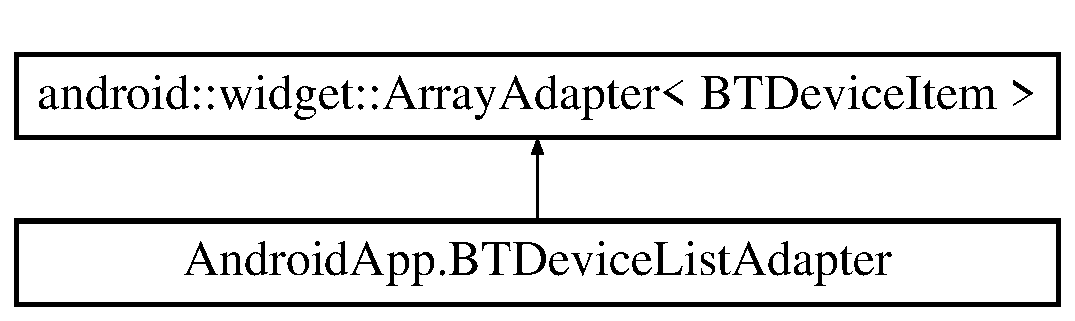
\includegraphics[height=2.000000cm]{class_android_app_1_1_b_t_device_list_adapter}
\end{center}
\end{figure}
\subsection*{Classes}
\begin{DoxyCompactItemize}
\item 
class \hyperlink{class_android_app_1_1_b_t_device_list_adapter_1_1_view_holder}{View\+Holder}
\begin{DoxyCompactList}\small\item\em Class that holds all data displayed for each List\+Item. \end{DoxyCompactList}\end{DoxyCompactItemize}
\subsection*{Public Member Functions}
\begin{DoxyCompactItemize}
\item 
\hyperlink{class_android_app_1_1_b_t_device_list_adapter_a6d4d0dc1f894bbb2378a71eea4907bb0}{B\+T\+Device\+List\+Adapter} (Context cnt, int \hyperlink{class_android_app_1_1_b_t_device_list_adapter_ae0c8b1482e416a5b242dcec87b83f661}{layout\+Resource\+Id}, Array\+List$<$ \hyperlink{class_android_app_1_1_b_t_device_item}{B\+T\+Device\+Item} $>$ \hyperlink{class_android_app_1_1_b_t_device_list_adapter_a210dbb300083d9029aa960841c8aa505}{data})
\begin{DoxyCompactList}\small\item\em Constructor for the List\+View adapter. \end{DoxyCompactList}\item 
View \hyperlink{class_android_app_1_1_b_t_device_list_adapter_a3e2ad44a1c55bddc7102aa36ab18ddb0}{get\+View} (int position, View convert\+View, View\+Group parent)
\begin{DoxyCompactList}\small\item\em Function for returning the view of each list item (\hyperlink{class_android_app_1_1_b_t_device_item}{B\+T\+Device\+Item}). \end{DoxyCompactList}\end{DoxyCompactItemize}
\subsection*{Private Attributes}
\begin{DoxyCompactItemize}
\item 
\mbox{\Hypertarget{class_android_app_1_1_b_t_device_list_adapter_ae0c8b1482e416a5b242dcec87b83f661}\label{class_android_app_1_1_b_t_device_list_adapter_ae0c8b1482e416a5b242dcec87b83f661}} 
int \hyperlink{class_android_app_1_1_b_t_device_list_adapter_ae0c8b1482e416a5b242dcec87b83f661}{layout\+Resource\+Id}
\begin{DoxyCompactList}\small\item\em Resource ID for current layout. \end{DoxyCompactList}\item 
\mbox{\Hypertarget{class_android_app_1_1_b_t_device_list_adapter_a6ede6626d5bc086d094f35071f8d59c8}\label{class_android_app_1_1_b_t_device_list_adapter_a6ede6626d5bc086d094f35071f8d59c8}} 
Context \hyperlink{class_android_app_1_1_b_t_device_list_adapter_a6ede6626d5bc086d094f35071f8d59c8}{context}
\begin{DoxyCompactList}\small\item\em Context that the List\+View is operating in. \end{DoxyCompactList}\item 
\mbox{\Hypertarget{class_android_app_1_1_b_t_device_list_adapter_a210dbb300083d9029aa960841c8aa505}\label{class_android_app_1_1_b_t_device_list_adapter_a210dbb300083d9029aa960841c8aa505}} 
Array\+List$<$ \hyperlink{class_android_app_1_1_b_t_device_item}{B\+T\+Device\+Item} $>$ \hyperlink{class_android_app_1_1_b_t_device_list_adapter_a210dbb300083d9029aa960841c8aa505}{data}
\begin{DoxyCompactList}\small\item\em Array\+List of all bluetooth device items to display. \end{DoxyCompactList}\end{DoxyCompactItemize}


\subsection{Detailed Description}
Adapter class used for displaying bluetooth devices. 

\subsection{Constructor \& Destructor Documentation}
\mbox{\Hypertarget{class_android_app_1_1_b_t_device_list_adapter_a6d4d0dc1f894bbb2378a71eea4907bb0}\label{class_android_app_1_1_b_t_device_list_adapter_a6d4d0dc1f894bbb2378a71eea4907bb0}} 
\index{Android\+App\+::\+B\+T\+Device\+List\+Adapter@{Android\+App\+::\+B\+T\+Device\+List\+Adapter}!B\+T\+Device\+List\+Adapter@{B\+T\+Device\+List\+Adapter}}
\index{B\+T\+Device\+List\+Adapter@{B\+T\+Device\+List\+Adapter}!Android\+App\+::\+B\+T\+Device\+List\+Adapter@{Android\+App\+::\+B\+T\+Device\+List\+Adapter}}
\subsubsection{\texorpdfstring{B\+T\+Device\+List\+Adapter()}{BTDeviceListAdapter()}}
{\footnotesize\ttfamily Android\+App.\+B\+T\+Device\+List\+Adapter.\+B\+T\+Device\+List\+Adapter (\begin{DoxyParamCaption}\item[{Context}]{cnt,  }\item[{int}]{layout\+Resource\+Id,  }\item[{Array\+List$<$ \hyperlink{class_android_app_1_1_b_t_device_item}{B\+T\+Device\+Item} $>$}]{data }\end{DoxyParamCaption})\hspace{0.3cm}{\ttfamily [inline]}}



Constructor for the List\+View adapter. 

Calls the constructor of the superclass as well as setting other relevant information needed.


\begin{DoxyParams}{Parameters}
{\em cnt} & -\/ Context of the adapter to be operating in. \\
\hline
{\em layout\+Resource\+Id} & -\/ Resource ID for current layout. \\
\hline
{\em data} & -\/ Array\+List of devices to display in List\+View. \\
\hline
\end{DoxyParams}

\begin{DoxyCode}
51                                                                                                 \{
52         super(cnt, \hyperlink{class_android_app_1_1_b_t_device_list_adapter_ae0c8b1482e416a5b242dcec87b83f661}{layoutResourceId}, \hyperlink{class_android_app_1_1_b_t_device_list_adapter_a210dbb300083d9029aa960841c8aa505}{data});
53         this.\hyperlink{class_android_app_1_1_b_t_device_list_adapter_a6ede6626d5bc086d094f35071f8d59c8}{context} = cnt;
54         this.\hyperlink{class_android_app_1_1_b_t_device_list_adapter_ae0c8b1482e416a5b242dcec87b83f661}{layoutResourceId} = \hyperlink{class_android_app_1_1_b_t_device_list_adapter_ae0c8b1482e416a5b242dcec87b83f661}{layoutResourceId};
55         this.\hyperlink{class_android_app_1_1_b_t_device_list_adapter_a210dbb300083d9029aa960841c8aa505}{data} = \hyperlink{class_android_app_1_1_b_t_device_list_adapter_a210dbb300083d9029aa960841c8aa505}{data};
56     \}
\end{DoxyCode}


\subsection{Member Function Documentation}
\mbox{\Hypertarget{class_android_app_1_1_b_t_device_list_adapter_a3e2ad44a1c55bddc7102aa36ab18ddb0}\label{class_android_app_1_1_b_t_device_list_adapter_a3e2ad44a1c55bddc7102aa36ab18ddb0}} 
\index{Android\+App\+::\+B\+T\+Device\+List\+Adapter@{Android\+App\+::\+B\+T\+Device\+List\+Adapter}!get\+View@{get\+View}}
\index{get\+View@{get\+View}!Android\+App\+::\+B\+T\+Device\+List\+Adapter@{Android\+App\+::\+B\+T\+Device\+List\+Adapter}}
\subsubsection{\texorpdfstring{get\+View()}{getView()}}
{\footnotesize\ttfamily View Android\+App.\+B\+T\+Device\+List\+Adapter.\+get\+View (\begin{DoxyParamCaption}\item[{int}]{position,  }\item[{View}]{convert\+View,  }\item[{View\+Group}]{parent }\end{DoxyParamCaption})\hspace{0.3cm}{\ttfamily [inline]}}



Function for returning the view of each list item (\hyperlink{class_android_app_1_1_b_t_device_item}{B\+T\+Device\+Item}). 

If a view for selected item has not been created inflater initialises it. A holder is then used to hold all the information that will be displayed on the UI to the user.


\begin{DoxyParams}{Parameters}
{\em position} & -\/ Index of item in array to use/reference to. \\
\hline
{\em convert\+View} & -\/ View to be used for specified item. \\
\hline
{\em parent} & -\/ Object where the created view will be placed on. \\
\hline
\end{DoxyParams}
\begin{DoxyReturn}{Returns}
View -\/ The result view of item with updated/current information. 
\end{DoxyReturn}


References Android\+App.\+B\+T\+Device\+Item.\+get\+Device(), Android\+App.\+B\+T\+Device\+Item.\+get\+Icon\+I\+D(), and Android\+App.\+B\+T\+Device\+Item.\+get\+Status().


\begin{DoxyCode}
82                                                                           \{
83 
84         ViewHolder holder;
85 
86         \textcolor{keywordflow}{if} (convertView == null)
87         \{
88             \textcolor{comment}{/* Create new view via inflater as it does not exist. */}
89             LayoutInflater inflater = (LayoutInflater)\hyperlink{class_android_app_1_1_b_t_device_list_adapter_a6ede6626d5bc086d094f35071f8d59c8}{context}.getSystemService(Context.
      LAYOUT\_INFLATER\_SERVICE);
90             convertView = inflater.inflate(\hyperlink{class_android_app_1_1_b_t_device_list_adapter_ae0c8b1482e416a5b242dcec87b83f661}{layoutResourceId}, parent, \textcolor{keyword}{false});
91 
92             \textcolor{comment}{/* Create holder that will contain information to display. */}
93             holder = \textcolor{keyword}{new} ViewHolder();
94             holder.imageStatus = (ImageView)convertView.findViewById(R.id.imageListStatus);
95             holder.name = (TextView)convertView.findViewById(R.id.textListName);
96             holder.address = (TextView)convertView.findViewById(R.id.textListAddress);
97             holder.status = (TextView)convertView.findViewById(R.id.textListStatus);
98             convertView.setTag(holder);
99         \}
100         \textcolor{keywordflow}{else}
101         \{
102             \textcolor{comment}{/* Get current holder to use instead of creating new one. */}
103             holder = (ViewHolder)convertView.getTag();
104         \}
105 
106         \textcolor{comment}{/* Get BTDeviceItem for specified item and update holder info. */}
107         BTDeviceItem btItem = getItem(position);
108         holder.imageStatus.setImageResource(btItem.getIconID());
109         holder.name.setText(btItem.getDevice().getName());
110         holder.address.setText(btItem.getDevice().getAddress());
111         holder.status.setText(btItem.getStatus());
112 
113         \textcolor{keywordflow}{return} convertView;
114     \}
\end{DoxyCode}


The documentation for this class was generated from the following file\+:\begin{DoxyCompactItemize}
\item 
android-\/app/app/src/main/java/com/jack/motorbikestatistics/\hyperlink{_b_t_device_list_adapter_8java}{B\+T\+Device\+List\+Adapter.\+java}\end{DoxyCompactItemize}

\hypertarget{class_android_app_1_1_b_t_device_list_adapter_1_1_view_holder}{}\section{Android\+App.\+B\+T\+Device\+List\+Adapter.\+View\+Holder Class Reference}
\label{class_android_app_1_1_b_t_device_list_adapter_1_1_view_holder}\index{Android\+App.\+B\+T\+Device\+List\+Adapter.\+View\+Holder@{Android\+App.\+B\+T\+Device\+List\+Adapter.\+View\+Holder}}


Class that holds all data displayed for each List\+Item.  




\subsection{Detailed Description}
Class that holds all data displayed for each List\+Item. 

The documentation for this class was generated from the following file\+:\begin{DoxyCompactItemize}
\item 
android-\/app/app/src/main/java/com/jack/motorbikestatistics/\hyperlink{_b_t_device_list_adapter_8java}{B\+T\+Device\+List\+Adapter.\+java}\end{DoxyCompactItemize}

\hypertarget{class_android_app_1_1_data_item}{}\section{Android\+App.\+Data\+Item$<$ T $>$ Class Template Reference}
\label{class_android_app_1_1_data_item}\index{Android\+App.\+Data\+Item$<$ T $>$@{Android\+App.\+Data\+Item$<$ T $>$}}


Class used for holding and displaying a piece of data within the statistic List\+View UI.  


\subsection*{Public Member Functions}
\begin{DoxyCompactItemize}
\item 
\hyperlink{class_android_app_1_1_data_item_a11dd3418028a213466ac1c075120de57}{Data\+Item} (String \hyperlink{class_android_app_1_1_data_item_a7e6d01c4d449403e707e99fce240b33b}{name}, boolean avg\+Min\+Max)
\begin{DoxyCompactList}\small\item\em Constructor for creation of a \hyperlink{class_android_app_1_1_data_item}{Data\+Item}. \end{DoxyCompactList}\item 
\hyperlink{class_android_app_1_1_data_item_a46a1d40afefec40e043301faefab4670}{Data\+Item} (String \hyperlink{class_android_app_1_1_data_item_a7e6d01c4d449403e707e99fce240b33b}{name}, boolean avg\+Min\+Max, T value)
\begin{DoxyCompactList}\small\item\em Constructor for creation of a \hyperlink{class_android_app_1_1_data_item}{Data\+Item}. \end{DoxyCompactList}\item 
String \hyperlink{class_android_app_1_1_data_item_adb968324854c42160f10bcf4ad05eec2}{get\+Name} ()
\begin{DoxyCompactList}\small\item\em Getter for name of data item. \end{DoxyCompactList}\item 
boolean \hyperlink{class_android_app_1_1_data_item_a45f09cabd91cc7032357b02bb0498c3e}{get\+Enabled\+Avg\+Min\+Max} ()
\begin{DoxyCompactList}\small\item\em Getter for whether additional functionality enabled. \end{DoxyCompactList}\item 
T \hyperlink{class_android_app_1_1_data_item_aee0b56933fb8673f7b6e52cde9da157c}{get\+Current} ()
\begin{DoxyCompactList}\small\item\em Getter for current reading value. \end{DoxyCompactList}\item 
Double \hyperlink{class_android_app_1_1_data_item_ad3b598a42bc7e38aa46d5091a752a47b}{get\+Average} ()
\begin{DoxyCompactList}\small\item\em Getter for average of readings. \end{DoxyCompactList}\item 
T \hyperlink{class_android_app_1_1_data_item_a1acf18ed04f82adb18ff73f4ef70b863}{get\+Minimum} ()
\begin{DoxyCompactList}\small\item\em Getter for minimum of readings. \end{DoxyCompactList}\item 
T \hyperlink{class_android_app_1_1_data_item_abc05cb2c7e1c30a018191cb140afc948}{get\+Maximum} ()
\begin{DoxyCompactList}\small\item\em Getter for maximum of readings. \end{DoxyCompactList}\item 
void \hyperlink{class_android_app_1_1_data_item_a6cd8975067d5be2d5eaac137a94c0eac}{set\+Current} (T value)
\begin{DoxyCompactList}\small\item\em Setter for current reading value. \end{DoxyCompactList}\end{DoxyCompactItemize}
\subsection*{Private Member Functions}
\begin{DoxyCompactItemize}
\item 
Double \hyperlink{class_android_app_1_1_data_item_aef809535c5a50c48d521db5ee9f6f9a7}{add} (Number a, Number b)
\begin{DoxyCompactList}\small\item\em Function to allow addition of numbers with variable types. \end{DoxyCompactList}\item 
Double \hyperlink{class_android_app_1_1_data_item_a3c4b68091e69bed9af18df05d6ea26a5}{divide} (Number numerator, Number denominator)
\begin{DoxyCompactList}\small\item\em Function to allow division of numbers with variable types. \end{DoxyCompactList}\item 
boolean \hyperlink{class_android_app_1_1_data_item_ab7fc2c1c68ba314ce4131e3e761aef2e}{greater\+Than} (Number a, Number b)
\begin{DoxyCompactList}\small\item\em Function to chcek whether A is greater than B. \end{DoxyCompactList}\item 
boolean \hyperlink{class_android_app_1_1_data_item_a94d948e8d1922c116246402c633109fc}{less\+Than} (Number a, Number b)
\begin{DoxyCompactList}\small\item\em Function to chcek whether A is less than B. \end{DoxyCompactList}\end{DoxyCompactItemize}
\subsection*{Private Attributes}
\begin{DoxyCompactItemize}
\item 
\mbox{\Hypertarget{class_android_app_1_1_data_item_a7e6d01c4d449403e707e99fce240b33b}\label{class_android_app_1_1_data_item_a7e6d01c4d449403e707e99fce240b33b}} 
String \hyperlink{class_android_app_1_1_data_item_a7e6d01c4d449403e707e99fce240b33b}{name}
\begin{DoxyCompactList}\small\item\em The name of the statistic. \end{DoxyCompactList}\item 
\mbox{\Hypertarget{class_android_app_1_1_data_item_a330d3ade00b732f202d73dbb0d3b711f}\label{class_android_app_1_1_data_item_a330d3ade00b732f202d73dbb0d3b711f}} 
boolean \hyperlink{class_android_app_1_1_data_item_a330d3ade00b732f202d73dbb0d3b711f}{enable\+Avg\+Min\+Max}
\begin{DoxyCompactList}\small\item\em Whether averaging, min \& max values should be calculated. \end{DoxyCompactList}\item 
\mbox{\Hypertarget{class_android_app_1_1_data_item_aef9fad1dca931e60708187ab89769f54}\label{class_android_app_1_1_data_item_aef9fad1dca931e60708187ab89769f54}} 
T \hyperlink{class_android_app_1_1_data_item_aef9fad1dca931e60708187ab89769f54}{current} = null
\begin{DoxyCompactList}\small\item\em Current reading value. \end{DoxyCompactList}\item 
\mbox{\Hypertarget{class_android_app_1_1_data_item_a231634a35289bb35c46f7fa3111cd472}\label{class_android_app_1_1_data_item_a231634a35289bb35c46f7fa3111cd472}} 
Double \hyperlink{class_android_app_1_1_data_item_a231634a35289bb35c46f7fa3111cd472}{average} = 0.\+0
\begin{DoxyCompactList}\small\item\em Average reading value. \end{DoxyCompactList}\item 
\mbox{\Hypertarget{class_android_app_1_1_data_item_aa146ca811e2838ef5c5621c99c712cda}\label{class_android_app_1_1_data_item_aa146ca811e2838ef5c5621c99c712cda}} 
Double \hyperlink{class_android_app_1_1_data_item_aa146ca811e2838ef5c5621c99c712cda}{average\+Sum} = 0.\+0
\begin{DoxyCompactList}\small\item\em Sum of all readings, used for averaging. \end{DoxyCompactList}\item 
\mbox{\Hypertarget{class_android_app_1_1_data_item_ae8ac0338f533843c475fac5e6510ce5c}\label{class_android_app_1_1_data_item_ae8ac0338f533843c475fac5e6510ce5c}} 
int \hyperlink{class_android_app_1_1_data_item_ae8ac0338f533843c475fac5e6510ce5c}{average\+Count} = 0
\begin{DoxyCompactList}\small\item\em Number of readings, used for averaging. \end{DoxyCompactList}\item 
\mbox{\Hypertarget{class_android_app_1_1_data_item_a23e9e2f0dbcfe5e163cd57888ed3dbd7}\label{class_android_app_1_1_data_item_a23e9e2f0dbcfe5e163cd57888ed3dbd7}} 
T \hyperlink{class_android_app_1_1_data_item_a23e9e2f0dbcfe5e163cd57888ed3dbd7}{minimum} = null
\begin{DoxyCompactList}\small\item\em Minimum reading value. \end{DoxyCompactList}\item 
\mbox{\Hypertarget{class_android_app_1_1_data_item_a6e53719b27d08f889c4d6460254583dc}\label{class_android_app_1_1_data_item_a6e53719b27d08f889c4d6460254583dc}} 
T \hyperlink{class_android_app_1_1_data_item_a6e53719b27d08f889c4d6460254583dc}{maximum} = null
\begin{DoxyCompactList}\small\item\em Maximum reading value. \end{DoxyCompactList}\end{DoxyCompactItemize}


\subsection{Detailed Description}
Class used for holding and displaying a piece of data within the statistic List\+View UI. 

\subsection{Constructor \& Destructor Documentation}
\mbox{\Hypertarget{class_android_app_1_1_data_item_a11dd3418028a213466ac1c075120de57}\label{class_android_app_1_1_data_item_a11dd3418028a213466ac1c075120de57}} 
\index{Android\+App\+::\+Data\+Item@{Android\+App\+::\+Data\+Item}!Data\+Item@{Data\+Item}}
\index{Data\+Item@{Data\+Item}!Android\+App\+::\+Data\+Item@{Android\+App\+::\+Data\+Item}}
\subsubsection{\texorpdfstring{Data\+Item()}{DataItem()}\hspace{0.1cm}{\footnotesize\ttfamily [1/2]}}
{\footnotesize\ttfamily \hyperlink{class_android_app_1_1_data_item}{Android\+App.\+Data\+Item}$<$ T $>$.\hyperlink{class_android_app_1_1_data_item}{Data\+Item} (\begin{DoxyParamCaption}\item[{String}]{name,  }\item[{boolean}]{avg\+Min\+Max }\end{DoxyParamCaption})\hspace{0.3cm}{\ttfamily [inline]}}



Constructor for creation of a \hyperlink{class_android_app_1_1_data_item}{Data\+Item}. 

Sets up the name of the data item as well as Whether averaging, minimum and maximum readings will be used


\begin{DoxyParams}{Parameters}
{\em name} & -\/ Name of the data item. \\
\hline
{\em avg\+Min\+Max} & -\/ Whether additive functionality shall be available. \\
\hline
\end{DoxyParams}

\begin{DoxyCode}
48                                                     \{
49         this.\hyperlink{class_android_app_1_1_data_item_a7e6d01c4d449403e707e99fce240b33b}{name} = \hyperlink{class_android_app_1_1_data_item_a7e6d01c4d449403e707e99fce240b33b}{name};
50         this.\hyperlink{class_android_app_1_1_data_item_a330d3ade00b732f202d73dbb0d3b711f}{enableAvgMinMax} = avgMinMax;
51     \}
\end{DoxyCode}
\mbox{\Hypertarget{class_android_app_1_1_data_item_a46a1d40afefec40e043301faefab4670}\label{class_android_app_1_1_data_item_a46a1d40afefec40e043301faefab4670}} 
\index{Android\+App\+::\+Data\+Item@{Android\+App\+::\+Data\+Item}!Data\+Item@{Data\+Item}}
\index{Data\+Item@{Data\+Item}!Android\+App\+::\+Data\+Item@{Android\+App\+::\+Data\+Item}}
\subsubsection{\texorpdfstring{Data\+Item()}{DataItem()}\hspace{0.1cm}{\footnotesize\ttfamily [2/2]}}
{\footnotesize\ttfamily \hyperlink{class_android_app_1_1_data_item}{Android\+App.\+Data\+Item}$<$ T $>$.\hyperlink{class_android_app_1_1_data_item}{Data\+Item} (\begin{DoxyParamCaption}\item[{String}]{name,  }\item[{boolean}]{avg\+Min\+Max,  }\item[{T}]{value }\end{DoxyParamCaption})\hspace{0.3cm}{\ttfamily [inline]}}



Constructor for creation of a \hyperlink{class_android_app_1_1_data_item}{Data\+Item}. 

Similar to other constructor however allows setting of an initial value.


\begin{DoxyParams}{Parameters}
{\em name} & -\/ Name of the data item. \\
\hline
{\em avg\+Min\+Max} & -\/ Whether additive functionality shall be available. \\
\hline
{\em value} & -\/ Initial reading value. \\
\hline
\end{DoxyParams}

\begin{DoxyCode}
63                                                              \{
64         this.\hyperlink{class_android_app_1_1_data_item_a7e6d01c4d449403e707e99fce240b33b}{name} = \hyperlink{class_android_app_1_1_data_item_a7e6d01c4d449403e707e99fce240b33b}{name};
65         this.\hyperlink{class_android_app_1_1_data_item_a330d3ade00b732f202d73dbb0d3b711f}{enableAvgMinMax} = avgMinMax;
66         this.\hyperlink{class_android_app_1_1_data_item_aef9fad1dca931e60708187ab89769f54}{current} = value;
67 
68         \textcolor{keywordflow}{if} ((avgMinMax) && (\hyperlink{class_android_app_1_1_data_item_aef9fad1dca931e60708187ab89769f54}{current} instanceof Number)) \{
69             this.\hyperlink{class_android_app_1_1_data_item_a231634a35289bb35c46f7fa3111cd472}{average} = (Double)value;
70             this.\hyperlink{class_android_app_1_1_data_item_aa146ca811e2838ef5c5621c99c712cda}{averageSum} = (Double)value;
71             this.\hyperlink{class_android_app_1_1_data_item_ae8ac0338f533843c475fac5e6510ce5c}{averageCount}++;
72 
73             this.\hyperlink{class_android_app_1_1_data_item_a23e9e2f0dbcfe5e163cd57888ed3dbd7}{minimum} = value;
74             this.\hyperlink{class_android_app_1_1_data_item_a6e53719b27d08f889c4d6460254583dc}{maximum} = value;
75         \}
76     \}
\end{DoxyCode}


\subsection{Member Function Documentation}
\mbox{\Hypertarget{class_android_app_1_1_data_item_adb968324854c42160f10bcf4ad05eec2}\label{class_android_app_1_1_data_item_adb968324854c42160f10bcf4ad05eec2}} 
\index{Android\+App\+::\+Data\+Item@{Android\+App\+::\+Data\+Item}!get\+Name@{get\+Name}}
\index{get\+Name@{get\+Name}!Android\+App\+::\+Data\+Item@{Android\+App\+::\+Data\+Item}}
\subsubsection{\texorpdfstring{get\+Name()}{getName()}}
{\footnotesize\ttfamily String \hyperlink{class_android_app_1_1_data_item}{Android\+App.\+Data\+Item}$<$ T $>$.get\+Name (\begin{DoxyParamCaption}{ }\end{DoxyParamCaption})\hspace{0.3cm}{\ttfamily [inline]}}



Getter for name of data item. 

\begin{DoxyReturn}{Returns}
String -\/ \hyperlink{class_android_app_1_1_data_item}{Data\+Item} name. 
\end{DoxyReturn}

\begin{DoxyCode}
82                             \{
83         \textcolor{keywordflow}{return} \hyperlink{class_android_app_1_1_data_item_a7e6d01c4d449403e707e99fce240b33b}{name};
84     \}
\end{DoxyCode}
\mbox{\Hypertarget{class_android_app_1_1_data_item_a45f09cabd91cc7032357b02bb0498c3e}\label{class_android_app_1_1_data_item_a45f09cabd91cc7032357b02bb0498c3e}} 
\index{Android\+App\+::\+Data\+Item@{Android\+App\+::\+Data\+Item}!get\+Enabled\+Avg\+Min\+Max@{get\+Enabled\+Avg\+Min\+Max}}
\index{get\+Enabled\+Avg\+Min\+Max@{get\+Enabled\+Avg\+Min\+Max}!Android\+App\+::\+Data\+Item@{Android\+App\+::\+Data\+Item}}
\subsubsection{\texorpdfstring{get\+Enabled\+Avg\+Min\+Max()}{getEnabledAvgMinMax()}}
{\footnotesize\ttfamily boolean \hyperlink{class_android_app_1_1_data_item}{Android\+App.\+Data\+Item}$<$ T $>$.get\+Enabled\+Avg\+Min\+Max (\begin{DoxyParamCaption}{ }\end{DoxyParamCaption})\hspace{0.3cm}{\ttfamily [inline]}}



Getter for whether additional functionality enabled. 

\begin{DoxyReturn}{Returns}
boolean -\/ Averaging, Minimum \& Maximum enabled. 
\end{DoxyReturn}

\begin{DoxyCode}
90                                          \{
91         \textcolor{keywordflow}{return} \hyperlink{class_android_app_1_1_data_item_a330d3ade00b732f202d73dbb0d3b711f}{enableAvgMinMax};
92     \}
\end{DoxyCode}
\mbox{\Hypertarget{class_android_app_1_1_data_item_aee0b56933fb8673f7b6e52cde9da157c}\label{class_android_app_1_1_data_item_aee0b56933fb8673f7b6e52cde9da157c}} 
\index{Android\+App\+::\+Data\+Item@{Android\+App\+::\+Data\+Item}!get\+Current@{get\+Current}}
\index{get\+Current@{get\+Current}!Android\+App\+::\+Data\+Item@{Android\+App\+::\+Data\+Item}}
\subsubsection{\texorpdfstring{get\+Current()}{getCurrent()}}
{\footnotesize\ttfamily T \hyperlink{class_android_app_1_1_data_item}{Android\+App.\+Data\+Item}$<$ T $>$.get\+Current (\begin{DoxyParamCaption}{ }\end{DoxyParamCaption})\hspace{0.3cm}{\ttfamily [inline]}}



Getter for current reading value. 

\begin{DoxyReturn}{Returns}
T -\/ Current reading value. 
\end{DoxyReturn}

\begin{DoxyCode}
98                           \{
99         \textcolor{keywordflow}{return} \hyperlink{class_android_app_1_1_data_item_aef9fad1dca931e60708187ab89769f54}{current};
100     \}
\end{DoxyCode}
\mbox{\Hypertarget{class_android_app_1_1_data_item_ad3b598a42bc7e38aa46d5091a752a47b}\label{class_android_app_1_1_data_item_ad3b598a42bc7e38aa46d5091a752a47b}} 
\index{Android\+App\+::\+Data\+Item@{Android\+App\+::\+Data\+Item}!get\+Average@{get\+Average}}
\index{get\+Average@{get\+Average}!Android\+App\+::\+Data\+Item@{Android\+App\+::\+Data\+Item}}
\subsubsection{\texorpdfstring{get\+Average()}{getAverage()}}
{\footnotesize\ttfamily Double \hyperlink{class_android_app_1_1_data_item}{Android\+App.\+Data\+Item}$<$ T $>$.get\+Average (\begin{DoxyParamCaption}{ }\end{DoxyParamCaption})\hspace{0.3cm}{\ttfamily [inline]}}



Getter for average of readings. 

\begin{DoxyReturn}{Returns}
Double -\/ Average of all readings. 
\end{DoxyReturn}

\begin{DoxyCode}
106                                \{
107         \textcolor{keywordflow}{return} \hyperlink{class_android_app_1_1_data_item_a231634a35289bb35c46f7fa3111cd472}{average};
108     \}
\end{DoxyCode}
\mbox{\Hypertarget{class_android_app_1_1_data_item_a1acf18ed04f82adb18ff73f4ef70b863}\label{class_android_app_1_1_data_item_a1acf18ed04f82adb18ff73f4ef70b863}} 
\index{Android\+App\+::\+Data\+Item@{Android\+App\+::\+Data\+Item}!get\+Minimum@{get\+Minimum}}
\index{get\+Minimum@{get\+Minimum}!Android\+App\+::\+Data\+Item@{Android\+App\+::\+Data\+Item}}
\subsubsection{\texorpdfstring{get\+Minimum()}{getMinimum()}}
{\footnotesize\ttfamily T \hyperlink{class_android_app_1_1_data_item}{Android\+App.\+Data\+Item}$<$ T $>$.get\+Minimum (\begin{DoxyParamCaption}{ }\end{DoxyParamCaption})\hspace{0.3cm}{\ttfamily [inline]}}



Getter for minimum of readings. 

\begin{DoxyReturn}{Returns}
T -\/ Minimum value. 
\end{DoxyReturn}

\begin{DoxyCode}
114                           \{
115         \textcolor{keywordflow}{return} \hyperlink{class_android_app_1_1_data_item_a23e9e2f0dbcfe5e163cd57888ed3dbd7}{minimum};
116     \}
\end{DoxyCode}
\mbox{\Hypertarget{class_android_app_1_1_data_item_abc05cb2c7e1c30a018191cb140afc948}\label{class_android_app_1_1_data_item_abc05cb2c7e1c30a018191cb140afc948}} 
\index{Android\+App\+::\+Data\+Item@{Android\+App\+::\+Data\+Item}!get\+Maximum@{get\+Maximum}}
\index{get\+Maximum@{get\+Maximum}!Android\+App\+::\+Data\+Item@{Android\+App\+::\+Data\+Item}}
\subsubsection{\texorpdfstring{get\+Maximum()}{getMaximum()}}
{\footnotesize\ttfamily T \hyperlink{class_android_app_1_1_data_item}{Android\+App.\+Data\+Item}$<$ T $>$.get\+Maximum (\begin{DoxyParamCaption}{ }\end{DoxyParamCaption})\hspace{0.3cm}{\ttfamily [inline]}}



Getter for maximum of readings. 

\begin{DoxyReturn}{Returns}
T -\/ Maximum value. 
\end{DoxyReturn}

\begin{DoxyCode}
122                           \{
123         \textcolor{keywordflow}{return} \hyperlink{class_android_app_1_1_data_item_a6e53719b27d08f889c4d6460254583dc}{maximum};
124     \}
\end{DoxyCode}
\mbox{\Hypertarget{class_android_app_1_1_data_item_a6cd8975067d5be2d5eaac137a94c0eac}\label{class_android_app_1_1_data_item_a6cd8975067d5be2d5eaac137a94c0eac}} 
\index{Android\+App\+::\+Data\+Item@{Android\+App\+::\+Data\+Item}!set\+Current@{set\+Current}}
\index{set\+Current@{set\+Current}!Android\+App\+::\+Data\+Item@{Android\+App\+::\+Data\+Item}}
\subsubsection{\texorpdfstring{set\+Current()}{setCurrent()}}
{\footnotesize\ttfamily void \hyperlink{class_android_app_1_1_data_item}{Android\+App.\+Data\+Item}$<$ T $>$.set\+Current (\begin{DoxyParamCaption}\item[{T}]{value }\end{DoxyParamCaption})\hspace{0.3cm}{\ttfamily [inline]}}



Setter for current reading value. 

If additive functionality enabled and the reading is of types number then we go ahead and update our min, max \& average values as well will the passed in new reading.


\begin{DoxyParams}{Parameters}
{\em T} & -\/ New reading. \\
\hline
\end{DoxyParams}

\begin{DoxyCode}
135                                     \{
136         this.\hyperlink{class_android_app_1_1_data_item_aef9fad1dca931e60708187ab89769f54}{current} = value;
137 
138         \textcolor{keywordflow}{if} ((\hyperlink{class_android_app_1_1_data_item_a330d3ade00b732f202d73dbb0d3b711f}{enableAvgMinMax}) && (\hyperlink{class_android_app_1_1_data_item_aef9fad1dca931e60708187ab89769f54}{current} instanceof Number)) \{
139 
140             \textcolor{comment}{/* Sets the average */}
141             \hyperlink{class_android_app_1_1_data_item_ae8ac0338f533843c475fac5e6510ce5c}{averageCount}++;
142             \hyperlink{class_android_app_1_1_data_item_aa146ca811e2838ef5c5621c99c712cda}{averageSum} = \hyperlink{class_android_app_1_1_data_item_aef809535c5a50c48d521db5ee9f6f9a7}{add}(\hyperlink{class_android_app_1_1_data_item_aa146ca811e2838ef5c5621c99c712cda}{averageSum}, (Number)value);
143             \hyperlink{class_android_app_1_1_data_item_a231634a35289bb35c46f7fa3111cd472}{average} = \hyperlink{class_android_app_1_1_data_item_a3c4b68091e69bed9af18df05d6ea26a5}{divide}(\hyperlink{class_android_app_1_1_data_item_aa146ca811e2838ef5c5621c99c712cda}{averageSum}, \hyperlink{class_android_app_1_1_data_item_ae8ac0338f533843c475fac5e6510ce5c}{averageCount});
144 
145             \textcolor{comment}{/* Sets the new minimum and maximums if true */}
146             \textcolor{keywordflow}{if} ((\hyperlink{class_android_app_1_1_data_item_a23e9e2f0dbcfe5e163cd57888ed3dbd7}{minimum} == null) || \hyperlink{class_android_app_1_1_data_item_a94d948e8d1922c116246402c633109fc}{lessThan}((Number)\hyperlink{class_android_app_1_1_data_item_aef9fad1dca931e60708187ab89769f54}{current}, (Number)
      \hyperlink{class_android_app_1_1_data_item_a23e9e2f0dbcfe5e163cd57888ed3dbd7}{minimum})) \{
147                 minimum = \hyperlink{class_android_app_1_1_data_item_aef9fad1dca931e60708187ab89769f54}{current};
148             \}
149             \textcolor{keywordflow}{if} ((\hyperlink{class_android_app_1_1_data_item_a6e53719b27d08f889c4d6460254583dc}{maximum} == null) || \hyperlink{class_android_app_1_1_data_item_ab7fc2c1c68ba314ce4131e3e761aef2e}{greaterThan}((Number)current, (Number)
      \hyperlink{class_android_app_1_1_data_item_a6e53719b27d08f889c4d6460254583dc}{maximum})) \{
150                 maximum = \hyperlink{class_android_app_1_1_data_item_aef9fad1dca931e60708187ab89769f54}{current};
151             \}
152         \}
153     \}
\end{DoxyCode}
\mbox{\Hypertarget{class_android_app_1_1_data_item_aef809535c5a50c48d521db5ee9f6f9a7}\label{class_android_app_1_1_data_item_aef809535c5a50c48d521db5ee9f6f9a7}} 
\index{Android\+App\+::\+Data\+Item@{Android\+App\+::\+Data\+Item}!add@{add}}
\index{add@{add}!Android\+App\+::\+Data\+Item@{Android\+App\+::\+Data\+Item}}
\subsubsection{\texorpdfstring{add()}{add()}}
{\footnotesize\ttfamily Double \hyperlink{class_android_app_1_1_data_item}{Android\+App.\+Data\+Item}$<$ T $>$.add (\begin{DoxyParamCaption}\item[{Number}]{a,  }\item[{Number}]{b }\end{DoxyParamCaption})\hspace{0.3cm}{\ttfamily [inline]}, {\ttfamily [private]}}



Function to allow addition of numbers with variable types. 


\begin{DoxyParams}{Parameters}
{\em a} & -\/ First operand. \\
\hline
{\em b} & -\/ Second operand. \\
\hline
\end{DoxyParams}
\begin{DoxyReturn}{Returns}
Double -\/ Sum. 
\end{DoxyReturn}

\begin{DoxyCode}
161                                            \{
162         \textcolor{keywordflow}{return} \textcolor{keyword}{new} Double(a.doubleValue() + b.doubleValue());
163     \}
\end{DoxyCode}
\mbox{\Hypertarget{class_android_app_1_1_data_item_a3c4b68091e69bed9af18df05d6ea26a5}\label{class_android_app_1_1_data_item_a3c4b68091e69bed9af18df05d6ea26a5}} 
\index{Android\+App\+::\+Data\+Item@{Android\+App\+::\+Data\+Item}!divide@{divide}}
\index{divide@{divide}!Android\+App\+::\+Data\+Item@{Android\+App\+::\+Data\+Item}}
\subsubsection{\texorpdfstring{divide()}{divide()}}
{\footnotesize\ttfamily Double \hyperlink{class_android_app_1_1_data_item}{Android\+App.\+Data\+Item}$<$ T $>$.divide (\begin{DoxyParamCaption}\item[{Number}]{numerator,  }\item[{Number}]{denominator }\end{DoxyParamCaption})\hspace{0.3cm}{\ttfamily [inline]}, {\ttfamily [private]}}



Function to allow division of numbers with variable types. 


\begin{DoxyParams}{Parameters}
{\em numerator} & -\/ Numerator of divisior. \\
\hline
{\em denominator} & -\/ Denominator of divisor. \\
\hline
\end{DoxyParams}
\begin{DoxyReturn}{Returns}
Double -\/ Result of division. 
\end{DoxyReturn}

\begin{DoxyCode}
171                                                                 \{
172         \textcolor{keywordflow}{return} \textcolor{keyword}{new} Double(numerator.doubleValue() / denominator.doubleValue());
173     \}
\end{DoxyCode}
\mbox{\Hypertarget{class_android_app_1_1_data_item_ab7fc2c1c68ba314ce4131e3e761aef2e}\label{class_android_app_1_1_data_item_ab7fc2c1c68ba314ce4131e3e761aef2e}} 
\index{Android\+App\+::\+Data\+Item@{Android\+App\+::\+Data\+Item}!greater\+Than@{greater\+Than}}
\index{greater\+Than@{greater\+Than}!Android\+App\+::\+Data\+Item@{Android\+App\+::\+Data\+Item}}
\subsubsection{\texorpdfstring{greater\+Than()}{greaterThan()}}
{\footnotesize\ttfamily boolean \hyperlink{class_android_app_1_1_data_item}{Android\+App.\+Data\+Item}$<$ T $>$.greater\+Than (\begin{DoxyParamCaption}\item[{Number}]{a,  }\item[{Number}]{b }\end{DoxyParamCaption})\hspace{0.3cm}{\ttfamily [inline]}, {\ttfamily [private]}}



Function to chcek whether A is greater than B. 


\begin{DoxyParams}{Parameters}
{\em a} & -\/ First operand. \\
\hline
{\em b} & -\/ Second operand. \\
\hline
\end{DoxyParams}
\begin{DoxyReturn}{Returns}
boolean -\/ Whether A is greater than B. 
\end{DoxyReturn}

\begin{DoxyCode}
181                                                     \{
182         \textcolor{keywordflow}{return} a.doubleValue() > b.doubleValue();
183     \}
\end{DoxyCode}
\mbox{\Hypertarget{class_android_app_1_1_data_item_a94d948e8d1922c116246402c633109fc}\label{class_android_app_1_1_data_item_a94d948e8d1922c116246402c633109fc}} 
\index{Android\+App\+::\+Data\+Item@{Android\+App\+::\+Data\+Item}!less\+Than@{less\+Than}}
\index{less\+Than@{less\+Than}!Android\+App\+::\+Data\+Item@{Android\+App\+::\+Data\+Item}}
\subsubsection{\texorpdfstring{less\+Than()}{lessThan()}}
{\footnotesize\ttfamily boolean \hyperlink{class_android_app_1_1_data_item}{Android\+App.\+Data\+Item}$<$ T $>$.less\+Than (\begin{DoxyParamCaption}\item[{Number}]{a,  }\item[{Number}]{b }\end{DoxyParamCaption})\hspace{0.3cm}{\ttfamily [inline]}, {\ttfamily [private]}}



Function to chcek whether A is less than B. 


\begin{DoxyParams}{Parameters}
{\em a} & -\/ First operand. \\
\hline
{\em b} & -\/ Second operand. \\
\hline
\end{DoxyParams}
\begin{DoxyReturn}{Returns}
boolean -\/ Whether A is less than B. 
\end{DoxyReturn}

\begin{DoxyCode}
191                                                  \{
192         \textcolor{keywordflow}{return} a.doubleValue() < b.doubleValue();
193     \}
\end{DoxyCode}


The documentation for this class was generated from the following file\+:\begin{DoxyCompactItemize}
\item 
android-\/app/app/src/main/java/com/jack/motorbikestatistics/\hyperlink{_data_item_8java}{Data\+Item.\+java}\end{DoxyCompactItemize}

\hypertarget{class_android_app_1_1_data_list_adapter}{}\section{Android\+App.\+Data\+List\+Adapter Class Reference}
\label{class_android_app_1_1_data_list_adapter}\index{Android\+App.\+Data\+List\+Adapter@{Android\+App.\+Data\+List\+Adapter}}


Adapter class used for displaying statistics.  


Inheritance diagram for Android\+App.\+Data\+List\+Adapter\+:\begin{figure}[H]
\begin{center}
\leavevmode
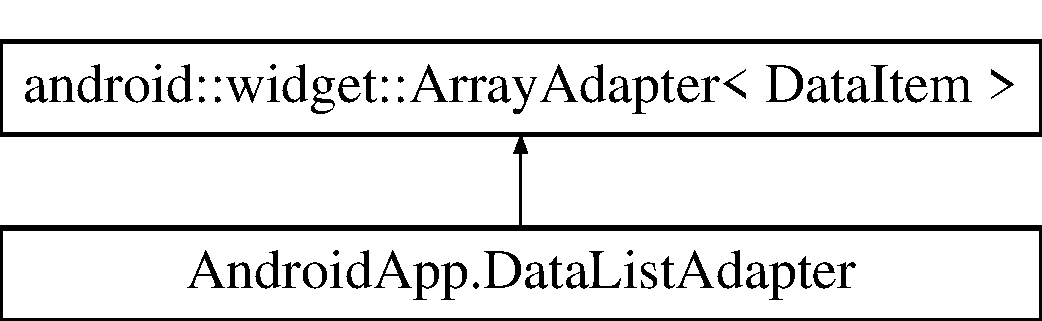
\includegraphics[height=2.000000cm]{class_android_app_1_1_data_list_adapter}
\end{center}
\end{figure}
\subsection*{Classes}
\begin{DoxyCompactItemize}
\item 
class \hyperlink{class_android_app_1_1_data_list_adapter_1_1_view_holder}{View\+Holder}
\begin{DoxyCompactList}\small\item\em Class that holds all data displayed for each List\+Item. \end{DoxyCompactList}\end{DoxyCompactItemize}
\subsection*{Public Member Functions}
\begin{DoxyCompactItemize}
\item 
\hyperlink{class_android_app_1_1_data_list_adapter_a654a6659bcdfdd08be0d7684269c1750}{Data\+List\+Adapter} (Context cnt, int \hyperlink{class_android_app_1_1_data_list_adapter_ac4680f2696f50995ecd43fa418f15524}{layout\+Resource\+Id}, Array\+List$<$ \hyperlink{class_android_app_1_1_data_item}{Data\+Item} $>$ \hyperlink{class_android_app_1_1_data_list_adapter_a733766e9ddd9f1cc3943dd83fc734c59}{data})
\begin{DoxyCompactList}\small\item\em Constructor for the List\+View adapter. \end{DoxyCompactList}\item 
View \hyperlink{class_android_app_1_1_data_list_adapter_acb1d33ad30608fff808765c10050f9c3}{get\+View} (int position, View convert\+View, View\+Group parent)
\begin{DoxyCompactList}\small\item\em Function for returning the view of each list item (\hyperlink{class_android_app_1_1_data_item}{Data\+Item}). \end{DoxyCompactList}\end{DoxyCompactItemize}
\subsection*{Private Attributes}
\begin{DoxyCompactItemize}
\item 
\mbox{\Hypertarget{class_android_app_1_1_data_list_adapter_a739dc817ded5d59af25f97be1a88cf75}\label{class_android_app_1_1_data_list_adapter_a739dc817ded5d59af25f97be1a88cf75}} 
Context \hyperlink{class_android_app_1_1_data_list_adapter_a739dc817ded5d59af25f97be1a88cf75}{context}
\begin{DoxyCompactList}\small\item\em Context that the List\+View is operating in. \end{DoxyCompactList}\item 
\mbox{\Hypertarget{class_android_app_1_1_data_list_adapter_ac4680f2696f50995ecd43fa418f15524}\label{class_android_app_1_1_data_list_adapter_ac4680f2696f50995ecd43fa418f15524}} 
int \hyperlink{class_android_app_1_1_data_list_adapter_ac4680f2696f50995ecd43fa418f15524}{layout\+Resource\+Id}
\begin{DoxyCompactList}\small\item\em Resource ID for current layout. \end{DoxyCompactList}\item 
\mbox{\Hypertarget{class_android_app_1_1_data_list_adapter_a733766e9ddd9f1cc3943dd83fc734c59}\label{class_android_app_1_1_data_list_adapter_a733766e9ddd9f1cc3943dd83fc734c59}} 
Array\+List$<$ \hyperlink{class_android_app_1_1_data_item}{Data\+Item} $>$ \hyperlink{class_android_app_1_1_data_list_adapter_a733766e9ddd9f1cc3943dd83fc734c59}{data}
\begin{DoxyCompactList}\small\item\em Array\+List of all statistic items to display. \end{DoxyCompactList}\end{DoxyCompactItemize}


\subsection{Detailed Description}
Adapter class used for displaying statistics. 

\subsection{Constructor \& Destructor Documentation}
\mbox{\Hypertarget{class_android_app_1_1_data_list_adapter_a654a6659bcdfdd08be0d7684269c1750}\label{class_android_app_1_1_data_list_adapter_a654a6659bcdfdd08be0d7684269c1750}} 
\index{Android\+App\+::\+Data\+List\+Adapter@{Android\+App\+::\+Data\+List\+Adapter}!Data\+List\+Adapter@{Data\+List\+Adapter}}
\index{Data\+List\+Adapter@{Data\+List\+Adapter}!Android\+App\+::\+Data\+List\+Adapter@{Android\+App\+::\+Data\+List\+Adapter}}
\subsubsection{\texorpdfstring{Data\+List\+Adapter()}{DataListAdapter()}}
{\footnotesize\ttfamily Android\+App.\+Data\+List\+Adapter.\+Data\+List\+Adapter (\begin{DoxyParamCaption}\item[{Context}]{cnt,  }\item[{int}]{layout\+Resource\+Id,  }\item[{Array\+List$<$ \hyperlink{class_android_app_1_1_data_item}{Data\+Item} $>$}]{data }\end{DoxyParamCaption})\hspace{0.3cm}{\ttfamily [inline]}}



Constructor for the List\+View adapter. 

Calls the constructor of the superclass as well as setting other relevant information needed.


\begin{DoxyParams}{Parameters}
{\em cnt} & -\/ Context of the adapter to be operating in. \\
\hline
{\em layout\+Resource\+Id} & -\/ Resource ID for current layout. \\
\hline
{\em data} & -\/ Array\+List of statistics to display in List\+View. \\
\hline
\end{DoxyParams}

\begin{DoxyCode}
47                                                                                         \{
48         super(cnt, \hyperlink{class_android_app_1_1_data_list_adapter_ac4680f2696f50995ecd43fa418f15524}{layoutResourceId}, \hyperlink{class_android_app_1_1_data_list_adapter_a733766e9ddd9f1cc3943dd83fc734c59}{data});
49 
50         this.\hyperlink{class_android_app_1_1_data_list_adapter_a739dc817ded5d59af25f97be1a88cf75}{context} = cnt;
51         this.\hyperlink{class_android_app_1_1_data_list_adapter_ac4680f2696f50995ecd43fa418f15524}{layoutResourceId} = \hyperlink{class_android_app_1_1_data_list_adapter_ac4680f2696f50995ecd43fa418f15524}{layoutResourceId};
52         this.\hyperlink{class_android_app_1_1_data_list_adapter_a733766e9ddd9f1cc3943dd83fc734c59}{data} = \hyperlink{class_android_app_1_1_data_list_adapter_a733766e9ddd9f1cc3943dd83fc734c59}{data};
53     \}
\end{DoxyCode}


\subsection{Member Function Documentation}
\mbox{\Hypertarget{class_android_app_1_1_data_list_adapter_acb1d33ad30608fff808765c10050f9c3}\label{class_android_app_1_1_data_list_adapter_acb1d33ad30608fff808765c10050f9c3}} 
\index{Android\+App\+::\+Data\+List\+Adapter@{Android\+App\+::\+Data\+List\+Adapter}!get\+View@{get\+View}}
\index{get\+View@{get\+View}!Android\+App\+::\+Data\+List\+Adapter@{Android\+App\+::\+Data\+List\+Adapter}}
\subsubsection{\texorpdfstring{get\+View()}{getView()}}
{\footnotesize\ttfamily View Android\+App.\+Data\+List\+Adapter.\+get\+View (\begin{DoxyParamCaption}\item[{int}]{position,  }\item[{View}]{convert\+View,  }\item[{View\+Group}]{parent }\end{DoxyParamCaption})\hspace{0.3cm}{\ttfamily [inline]}}



Function for returning the view of each list item (\hyperlink{class_android_app_1_1_data_item}{Data\+Item}). 

If a view for selected item has not been created inflater initialises it. A holder is then used to hold all the information that will be displayed on the UI to the user.


\begin{DoxyParams}{Parameters}
{\em position} & -\/ Index of item in array to use/reference to. \\
\hline
{\em convert\+View} & -\/ View to be used for specified item. \\
\hline
{\em parent} & -\/ Object where the created view will be placed on. \\
\hline
\end{DoxyParams}
\begin{DoxyReturn}{Returns}
View -\/ The result view of item with updated/current information. 
\end{DoxyReturn}


References Android\+App.\+Data\+Item$<$ T $>$.\+get\+Average(), Android\+App.\+Data\+Item$<$ T $>$.\+get\+Current(), Android\+App.\+Data\+Item$<$ T $>$.\+get\+Enabled\+Avg\+Min\+Max(), Android\+App.\+Data\+Item$<$ T $>$.\+get\+Maximum(), Android\+App.\+Data\+Item$<$ T $>$.\+get\+Minimum(), and Android\+App.\+Data\+Item$<$ T $>$.\+get\+Name().


\begin{DoxyCode}
80                                                                           \{
81 
82         ViewHolder holder;
83 
84         \textcolor{keywordflow}{if} (convertView == null)
85         \{
86             \textcolor{comment}{/* If view does not already exist. */}
87             LayoutInflater inflater = (LayoutInflater)\hyperlink{class_android_app_1_1_data_list_adapter_a739dc817ded5d59af25f97be1a88cf75}{context}.getSystemService(Context.
      LAYOUT\_INFLATER\_SERVICE);
88             convertView = inflater.inflate(\hyperlink{class_android_app_1_1_data_list_adapter_ac4680f2696f50995ecd43fa418f15524}{layoutResourceId}, parent, \textcolor{keyword}{false});
89 
90             holder = \textcolor{keyword}{new} ViewHolder();
91             holder.name = (TextView)convertView.findViewById(R.id.datalist\_name);
92             holder.current = (TextView)convertView.findViewById(R.id.datalist\_current);
93             holder.average = (TextView)convertView.findViewById(R.id.datalist\_average);
94             holder.minimum = (TextView)convertView.findViewById(R.id.datalist\_minimum);
95             holder.maximum = (TextView)convertView.findViewById(R.id.datalist\_maximum);
96             convertView.setTag(holder);
97         \}
98         \textcolor{keywordflow}{else}
99         \{
100             \textcolor{comment}{/* If view already exists. */}
101             holder = (ViewHolder)convertView.getTag();
102         \}
103 
104         DataItem dataItem = getItem(position);
105 
106         \textcolor{comment}{/* Set our holder with current data of item */}
107         holder.name.setText(dataItem.getName());
108 
109         Object current = dataItem.getCurrent();
110         \textcolor{keywordflow}{if} (current != null) \{
111             DecimalFormat df = \textcolor{keyword}{new} DecimalFormat(\textcolor{stringliteral}{"#.####"});
112             df.setRoundingMode(RoundingMode.CEILING);
113 
114             \textcolor{comment}{/* To aid aesthetics rounding is used. */}
115             \textcolor{keywordflow}{if} (current instanceof Double) \{
116                 holder.current.setText(df.format(current));
117             \} \textcolor{keywordflow}{else} \{
118                 holder.current.setText(current.toString());
119             \}
120 
121             \textcolor{comment}{/*}
122 \textcolor{comment}{             * Displays added functionality if available.}
123 \textcolor{comment}{             * Not all statistics need it, for example averaging of LAT/LNG.}
124 \textcolor{comment}{             */}
125             \textcolor{keywordflow}{if} (dataItem.getEnabledAvgMinMax()) \{
126                 holder.average.setText(df.format(dataItem.getAverage()));
127                 holder.minimum.setText(df.format(dataItem.getMinimum()));
128                 holder.maximum.setText(df.format(dataItem.getMaximum()));
129             \} \textcolor{keywordflow}{else} \{
130                 holder.average.setText(\textcolor{stringliteral}{"N/A"});
131                 holder.minimum.setText(\textcolor{stringliteral}{"N/A"});
132                 holder.maximum.setText(\textcolor{stringliteral}{"N/A"});
133             \}
134         \}
135 
136         \textcolor{keywordflow}{return} convertView;
137     \}
\end{DoxyCode}


The documentation for this class was generated from the following file\+:\begin{DoxyCompactItemize}
\item 
android-\/app/app/src/main/java/com/jack/motorbikestatistics/\hyperlink{_data_list_adapter_8java}{Data\+List\+Adapter.\+java}\end{DoxyCompactItemize}

\hypertarget{class_android_app_1_1_data_list_adapter_1_1_view_holder}{}\section{Android\+App.\+Data\+List\+Adapter.\+View\+Holder Class Reference}
\label{class_android_app_1_1_data_list_adapter_1_1_view_holder}\index{Android\+App.\+Data\+List\+Adapter.\+View\+Holder@{Android\+App.\+Data\+List\+Adapter.\+View\+Holder}}


Class that holds all data displayed for each List\+Item.  




\subsection{Detailed Description}
Class that holds all data displayed for each List\+Item. 

The documentation for this class was generated from the following file\+:\begin{DoxyCompactItemize}
\item 
android-\/app/app/src/main/java/com/jack/motorbikestatistics/\hyperlink{_data_list_adapter_8java}{Data\+List\+Adapter.\+java}\end{DoxyCompactItemize}

\hypertarget{class_android_app_1_1_j_s_o_n_handler_singleton}{}\section{Android\+App.\+J\+S\+O\+N\+Handler\+Singleton Class Reference}
\label{class_android_app_1_1_j_s_o_n_handler_singleton}\index{Android\+App.\+J\+S\+O\+N\+Handler\+Singleton@{Android\+App.\+J\+S\+O\+N\+Handler\+Singleton}}


Singleton class for holding all J\+S\+ON trip data.  


\subsection*{Static Public Member Functions}
\begin{DoxyCompactItemize}
\item 
static \hyperlink{class_android_app_1_1_j_s_o_n_handler_singleton}{J\+S\+O\+N\+Handler\+Singleton} \hyperlink{class_android_app_1_1_j_s_o_n_handler_singleton_a6b33b2582b9625f9ab0718013daa1aeb}{get\+Instance} ()
\begin{DoxyCompactList}\small\item\em Returns the instance of this singleton class. \end{DoxyCompactList}\end{DoxyCompactItemize}
\subsection*{Public Attributes}
\begin{DoxyCompactItemize}
\item 
\mbox{\Hypertarget{class_android_app_1_1_j_s_o_n_handler_singleton_ae4f5359d481ba862a6e77b9ec04615ee}\label{class_android_app_1_1_j_s_o_n_handler_singleton_ae4f5359d481ba862a6e77b9ec04615ee}} 
Array\+List$<$ J\+S\+O\+N\+Object $>$ {\bfseries trip\+Data}
\end{DoxyCompactItemize}
\subsection*{Private Member Functions}
\begin{DoxyCompactItemize}
\item 
\mbox{\Hypertarget{class_android_app_1_1_j_s_o_n_handler_singleton_a458ec5f08bf2da81be6dc852a065fcc2}\label{class_android_app_1_1_j_s_o_n_handler_singleton_a458ec5f08bf2da81be6dc852a065fcc2}} 
\hyperlink{class_android_app_1_1_j_s_o_n_handler_singleton_a458ec5f08bf2da81be6dc852a065fcc2}{J\+S\+O\+N\+Handler\+Singleton} ()
\begin{DoxyCompactList}\small\item\em Constructor for instance. Ensures Array\+List is initialised. \end{DoxyCompactList}\end{DoxyCompactItemize}
\subsection*{Static Private Attributes}
\begin{DoxyCompactItemize}
\item 
\mbox{\Hypertarget{class_android_app_1_1_j_s_o_n_handler_singleton_ac4e083a3f318072254453f69ea0efb88}\label{class_android_app_1_1_j_s_o_n_handler_singleton_ac4e083a3f318072254453f69ea0efb88}} 
static \hyperlink{class_android_app_1_1_j_s_o_n_handler_singleton}{J\+S\+O\+N\+Handler\+Singleton} {\bfseries our\+Instance} = new \hyperlink{class_android_app_1_1_j_s_o_n_handler_singleton}{J\+S\+O\+N\+Handler\+Singleton}()
\end{DoxyCompactItemize}


\subsection{Detailed Description}
Singleton class for holding all J\+S\+ON trip data. 

\subsection{Member Function Documentation}
\mbox{\Hypertarget{class_android_app_1_1_j_s_o_n_handler_singleton_a6b33b2582b9625f9ab0718013daa1aeb}\label{class_android_app_1_1_j_s_o_n_handler_singleton_a6b33b2582b9625f9ab0718013daa1aeb}} 
\index{Android\+App\+::\+J\+S\+O\+N\+Handler\+Singleton@{Android\+App\+::\+J\+S\+O\+N\+Handler\+Singleton}!get\+Instance@{get\+Instance}}
\index{get\+Instance@{get\+Instance}!Android\+App\+::\+J\+S\+O\+N\+Handler\+Singleton@{Android\+App\+::\+J\+S\+O\+N\+Handler\+Singleton}}
\subsubsection{\texorpdfstring{get\+Instance()}{getInstance()}}
{\footnotesize\ttfamily static \hyperlink{class_android_app_1_1_j_s_o_n_handler_singleton}{J\+S\+O\+N\+Handler\+Singleton} Android\+App.\+J\+S\+O\+N\+Handler\+Singleton.\+get\+Instance (\begin{DoxyParamCaption}{ }\end{DoxyParamCaption})\hspace{0.3cm}{\ttfamily [inline]}, {\ttfamily [static]}}



Returns the instance of this singleton class. 

\begin{DoxyReturn}{Returns}
J\+S\+O\+N\+Handle\+Singleton -\/ Instance of this class. 
\end{DoxyReturn}

\begin{DoxyCode}
31                                                      \{
32         \textcolor{keywordflow}{return} ourInstance;
33     \}
\end{DoxyCode}


The documentation for this class was generated from the following file\+:\begin{DoxyCompactItemize}
\item 
android-\/app/app/src/main/java/com/jack/motorbikestatistics/\hyperlink{_j_s_o_n_handler_singleton_8java}{J\+S\+O\+N\+Handler\+Singleton.\+java}\end{DoxyCompactItemize}

\hypertarget{class_android_app_1_1_load_device_fragment}{}\section{Android\+App.\+Load\+Device\+Fragment Class Reference}
\label{class_android_app_1_1_load_device_fragment}\index{Android\+App.\+Load\+Device\+Fragment@{Android\+App.\+Load\+Device\+Fragment}}


UI Class for loading saved trips from device.  


Inheritance diagram for Android\+App.\+Load\+Device\+Fragment\+:\begin{figure}[H]
\begin{center}
\leavevmode
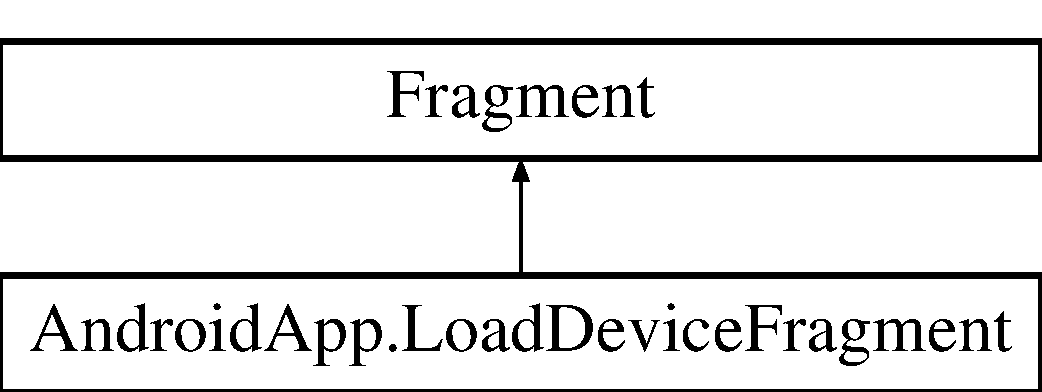
\includegraphics[height=2.000000cm]{class_android_app_1_1_load_device_fragment}
\end{center}
\end{figure}
\subsection*{Classes}
\begin{DoxyCompactItemize}
\item 
class \hyperlink{class_android_app_1_1_load_device_fragment_1_1_trip_item_listener}{Trip\+Item\+Listener}
\begin{DoxyCompactList}\small\item\em Listener used to identify when a trip has been pressed. \end{DoxyCompactList}\end{DoxyCompactItemize}
\subsection*{Public Member Functions}
\begin{DoxyCompactItemize}
\item 
\hyperlink{class_android_app_1_1_load_device_fragment_a2a090a4a947fb44a024a1d3c920b3b63}{Load\+Device\+Fragment} ()
\begin{DoxyCompactList}\small\item\em Constructor for UI fragment. \end{DoxyCompactList}\item 
View \hyperlink{class_android_app_1_1_load_device_fragment_af1a028ea902679e9bcc967c1b54b2451}{on\+Create\+View} (Layout\+Inflater inflater, View\+Group container, Bundle saved\+Instance\+State)
\begin{DoxyCompactList}\small\item\em Function called when fragment is shown on UI. \end{DoxyCompactList}\item 
void \hyperlink{class_android_app_1_1_load_device_fragment_a77ce93090f6c8c6aac522e35bfe9d21b}{set\+B\+T\+Connection} (\hyperlink{class_android_app_1_1_b_t_connection}{B\+T\+Connection} \hyperlink{class_android_app_1_1_load_device_fragment_a245147c7d3683cf1556680a382f328a9}{bt\+Connection})
\begin{DoxyCompactList}\small\item\em Setter for current BT connection. \end{DoxyCompactList}\end{DoxyCompactItemize}
\subsection*{Public Attributes}
\begin{DoxyCompactItemize}
\item 
final Handler \hyperlink{class_android_app_1_1_load_device_fragment_ad37565ea5a5332faf0c6b12284ca4e6c}{R\+X\+Handler}
\begin{DoxyCompactList}\small\item\em Handler used for receiving trip names. \end{DoxyCompactList}\end{DoxyCompactItemize}
\subsection*{Private Member Functions}
\begin{DoxyCompactItemize}
\item 
final void \hyperlink{class_android_app_1_1_load_device_fragment_a182949dc35ed68974acf64e20cdc6f20}{add\+Trip} (J\+S\+O\+N\+Object json\+Data)
\begin{DoxyCompactList}\small\item\em Adds a trip to the List\+View specifying name and filesize. \end{DoxyCompactList}\end{DoxyCompactItemize}
\subsection*{Private Attributes}
\begin{DoxyCompactItemize}
\item 
\mbox{\Hypertarget{class_android_app_1_1_load_device_fragment_a245147c7d3683cf1556680a382f328a9}\label{class_android_app_1_1_load_device_fragment_a245147c7d3683cf1556680a382f328a9}} 
\hyperlink{class_android_app_1_1_b_t_connection}{B\+T\+Connection} \hyperlink{class_android_app_1_1_load_device_fragment_a245147c7d3683cf1556680a382f328a9}{bt\+Connection} = null
\begin{DoxyCompactList}\small\item\em Current connectected logging device (via bluetooth). \end{DoxyCompactList}\item 
\mbox{\Hypertarget{class_android_app_1_1_load_device_fragment_a23e4856334c9782e15f7f7a08b544f4c}\label{class_android_app_1_1_load_device_fragment_a23e4856334c9782e15f7f7a08b544f4c}} 
Array\+List$<$ \hyperlink{class_android_app_1_1_trip_item}{Trip\+Item} $>$ \hyperlink{class_android_app_1_1_load_device_fragment_a23e4856334c9782e15f7f7a08b544f4c}{trip\+List}
\begin{DoxyCompactList}\small\item\em List of all trips saved on the logging device. \end{DoxyCompactList}\item 
\mbox{\Hypertarget{class_android_app_1_1_load_device_fragment_a96c2356cc65e934741c31ff3839ed9d3}\label{class_android_app_1_1_load_device_fragment_a96c2356cc65e934741c31ff3839ed9d3}} 
Array\+Adapter$<$ \hyperlink{class_android_app_1_1_trip_item}{Trip\+Item} $>$ \hyperlink{class_android_app_1_1_load_device_fragment_a96c2356cc65e934741c31ff3839ed9d3}{lv\+Adapter}
\begin{DoxyCompactList}\small\item\em Array adapter for displaying trips in List\+View. \end{DoxyCompactList}\end{DoxyCompactItemize}
\subsection*{Static Private Attributes}
\begin{DoxyCompactItemize}
\item 
\mbox{\Hypertarget{class_android_app_1_1_load_device_fragment_a4ceeef3ad914b52120973b83335a7b72}\label{class_android_app_1_1_load_device_fragment_a4ceeef3ad914b52120973b83335a7b72}} 
static final String \hyperlink{class_android_app_1_1_load_device_fragment_a4ceeef3ad914b52120973b83335a7b72}{N\+E\+W\+\_\+\+L\+I\+NE} = \char`\"{}\textbackslash{}r\textbackslash{}n\char`\"{}
\begin{DoxyCompactList}\small\item\em New line string. \end{DoxyCompactList}\item 
\mbox{\Hypertarget{class_android_app_1_1_load_device_fragment_afdfe423809d2267938f21eb4c5501653}\label{class_android_app_1_1_load_device_fragment_afdfe423809d2267938f21eb4c5501653}} 
static final String \hyperlink{class_android_app_1_1_load_device_fragment_afdfe423809d2267938f21eb4c5501653}{L\+O\+A\+D\+\_\+\+T\+R\+I\+P\+\_\+\+C\+H\+AR} = \char`\"{}3\char`\"{}
\begin{DoxyCompactList}\small\item\em Command string to be sent to device to load a specific trip. \end{DoxyCompactList}\end{DoxyCompactItemize}


\subsection{Detailed Description}
UI Class for loading saved trips from device. 

\subsection{Constructor \& Destructor Documentation}
\mbox{\Hypertarget{class_android_app_1_1_load_device_fragment_a2a090a4a947fb44a024a1d3c920b3b63}\label{class_android_app_1_1_load_device_fragment_a2a090a4a947fb44a024a1d3c920b3b63}} 
\index{Android\+App\+::\+Load\+Device\+Fragment@{Android\+App\+::\+Load\+Device\+Fragment}!Load\+Device\+Fragment@{Load\+Device\+Fragment}}
\index{Load\+Device\+Fragment@{Load\+Device\+Fragment}!Android\+App\+::\+Load\+Device\+Fragment@{Android\+App\+::\+Load\+Device\+Fragment}}
\subsubsection{\texorpdfstring{Load\+Device\+Fragment()}{LoadDeviceFragment()}}
{\footnotesize\ttfamily Android\+App.\+Load\+Device\+Fragment.\+Load\+Device\+Fragment (\begin{DoxyParamCaption}{ }\end{DoxyParamCaption})\hspace{0.3cm}{\ttfamily [inline]}}



Constructor for UI fragment. 

Creates a new arraylist of trips that is empty and ready to be filled from the logging device. 
\begin{DoxyCode}
55                                 \{
56         \hyperlink{class_android_app_1_1_load_device_fragment_a23e4856334c9782e15f7f7a08b544f4c}{tripList} = \textcolor{keyword}{new} ArrayList<TripItem>();
57     \}
\end{DoxyCode}


\subsection{Member Function Documentation}
\mbox{\Hypertarget{class_android_app_1_1_load_device_fragment_af1a028ea902679e9bcc967c1b54b2451}\label{class_android_app_1_1_load_device_fragment_af1a028ea902679e9bcc967c1b54b2451}} 
\index{Android\+App\+::\+Load\+Device\+Fragment@{Android\+App\+::\+Load\+Device\+Fragment}!on\+Create\+View@{on\+Create\+View}}
\index{on\+Create\+View@{on\+Create\+View}!Android\+App\+::\+Load\+Device\+Fragment@{Android\+App\+::\+Load\+Device\+Fragment}}
\subsubsection{\texorpdfstring{on\+Create\+View()}{onCreateView()}}
{\footnotesize\ttfamily View Android\+App.\+Load\+Device\+Fragment.\+on\+Create\+View (\begin{DoxyParamCaption}\item[{Layout\+Inflater}]{inflater,  }\item[{View\+Group}]{container,  }\item[{Bundle}]{saved\+Instance\+State }\end{DoxyParamCaption})\hspace{0.3cm}{\ttfamily [inline]}}



Function called when fragment is shown on UI. 

Sets up the List\+View on the screen using our custom Array\+Adapter specificed.


\begin{DoxyParams}{Parameters}
{\em inflater} & -\/ Inflater used to load fragment on UI. \\
\hline
{\em container} & -\/ Container where fragment will be shown. \\
\hline
{\em saved\+Instance\+State} & -\/ Information holding past state. \\
\hline
\end{DoxyParams}
\begin{DoxyReturn}{Returns}
View -\/ Modified view to display on the UI. 
\end{DoxyReturn}

\begin{DoxyCode}
72                                                                                                       \{
73         View myView = inflater.inflate(R.layout.loaddevice\_layout, container, \textcolor{keyword}{false});
74 
75         \textcolor{comment}{/* Get our ListView via ID, set headers and create our ArrayAdapter for it */}
76         ListView lvTripList = (ListView)myView.findViewById(R.id.loaddevice\_triplist);
77         lvTripList.setOnItemClickListener(\textcolor{keyword}{new} TripItemListener());
78 
79         ViewGroup headerView = (ViewGroup)inflater.inflate(R.layout.trip\_list\_header, lvTripList, \textcolor{keyword}{false});
80         lvTripList.addHeaderView(headerView);
81 
82         \hyperlink{class_android_app_1_1_load_device_fragment_a96c2356cc65e934741c31ff3839ed9d3}{lvAdapter} = \textcolor{keyword}{new} TripListAdapter(getActivity(), R.layout.trip\_list\_item, 
      \hyperlink{class_android_app_1_1_load_device_fragment_a23e4856334c9782e15f7f7a08b544f4c}{tripList});
83         lvTripList.setAdapter(\hyperlink{class_android_app_1_1_load_device_fragment_a96c2356cc65e934741c31ff3839ed9d3}{lvAdapter});
84 
85         \hyperlink{class_android_app_1_1_load_device_fragment_a23e4856334c9782e15f7f7a08b544f4c}{tripList}.clear();
86         \hyperlink{class_android_app_1_1_load_device_fragment_a96c2356cc65e934741c31ff3839ed9d3}{lvAdapter}.notifyDataSetChanged();
87 
88         \textcolor{keywordflow}{return} myView;
89     \}
\end{DoxyCode}
\mbox{\Hypertarget{class_android_app_1_1_load_device_fragment_a77ce93090f6c8c6aac522e35bfe9d21b}\label{class_android_app_1_1_load_device_fragment_a77ce93090f6c8c6aac522e35bfe9d21b}} 
\index{Android\+App\+::\+Load\+Device\+Fragment@{Android\+App\+::\+Load\+Device\+Fragment}!set\+B\+T\+Connection@{set\+B\+T\+Connection}}
\index{set\+B\+T\+Connection@{set\+B\+T\+Connection}!Android\+App\+::\+Load\+Device\+Fragment@{Android\+App\+::\+Load\+Device\+Fragment}}
\subsubsection{\texorpdfstring{set\+B\+T\+Connection()}{setBTConnection()}}
{\footnotesize\ttfamily void Android\+App.\+Load\+Device\+Fragment.\+set\+B\+T\+Connection (\begin{DoxyParamCaption}\item[{\hyperlink{class_android_app_1_1_b_t_connection}{B\+T\+Connection}}]{bt\+Connection }\end{DoxyParamCaption})\hspace{0.3cm}{\ttfamily [inline]}}



Setter for current BT connection. 

Set from main UI activity, allows cross tab communication with the logging device.


\begin{DoxyParams}{Parameters}
{\em bt\+Connection} & -\/ Logging device bluetooth connection. \\
\hline
\end{DoxyParams}

\begin{DoxyCode}
99                                                            \{
100         this.\hyperlink{class_android_app_1_1_load_device_fragment_a245147c7d3683cf1556680a382f328a9}{btConnection} = \hyperlink{class_android_app_1_1_load_device_fragment_a245147c7d3683cf1556680a382f328a9}{btConnection};
101     \}
\end{DoxyCode}
\mbox{\Hypertarget{class_android_app_1_1_load_device_fragment_a182949dc35ed68974acf64e20cdc6f20}\label{class_android_app_1_1_load_device_fragment_a182949dc35ed68974acf64e20cdc6f20}} 
\index{Android\+App\+::\+Load\+Device\+Fragment@{Android\+App\+::\+Load\+Device\+Fragment}!add\+Trip@{add\+Trip}}
\index{add\+Trip@{add\+Trip}!Android\+App\+::\+Load\+Device\+Fragment@{Android\+App\+::\+Load\+Device\+Fragment}}
\subsubsection{\texorpdfstring{add\+Trip()}{addTrip()}}
{\footnotesize\ttfamily final void Android\+App.\+Load\+Device\+Fragment.\+add\+Trip (\begin{DoxyParamCaption}\item[{J\+S\+O\+N\+Object}]{json\+Data }\end{DoxyParamCaption})\hspace{0.3cm}{\ttfamily [inline]}, {\ttfamily [private]}}



Adds a trip to the List\+View specifying name and filesize. 


\begin{DoxyParams}{Parameters}
{\em json\+Data} & -\/ J\+S\+ON object holding trip name and size. \\
\hline
\end{DoxyParams}

\begin{DoxyCode}
108                                                     \{
109         \textcolor{keywordflow}{try} \{
110 
111             \textcolor{comment}{/* Get name and size from json object */}
112             String tripName = jsonData.getString(\textcolor{stringliteral}{"name"});
113             \textcolor{keywordtype}{int} fileSize = jsonData.getInt(\textcolor{stringliteral}{"size"});
114 
115             \textcolor{comment}{/* Add new trip to our list & notify list view */}
116             TripItem newTrip = \textcolor{keyword}{new} TripItem(tripName, fileSize);
117             \hyperlink{class_android_app_1_1_load_device_fragment_a23e4856334c9782e15f7f7a08b544f4c}{tripList}.add(newTrip);
118             \hyperlink{class_android_app_1_1_load_device_fragment_a96c2356cc65e934741c31ff3839ed9d3}{lvAdapter}.notifyDataSetChanged();
119 
120         \} \textcolor{keywordflow}{catch} (JSONException e) \{
121             \textcolor{comment}{/* Do nothing */}
122         \}
123     \}
\end{DoxyCode}


\subsection{Member Data Documentation}
\mbox{\Hypertarget{class_android_app_1_1_load_device_fragment_ad37565ea5a5332faf0c6b12284ca4e6c}\label{class_android_app_1_1_load_device_fragment_ad37565ea5a5332faf0c6b12284ca4e6c}} 
\index{Android\+App\+::\+Load\+Device\+Fragment@{Android\+App\+::\+Load\+Device\+Fragment}!R\+X\+Handler@{R\+X\+Handler}}
\index{R\+X\+Handler@{R\+X\+Handler}!Android\+App\+::\+Load\+Device\+Fragment@{Android\+App\+::\+Load\+Device\+Fragment}}
\subsubsection{\texorpdfstring{R\+X\+Handler}{RXHandler}}
{\footnotesize\ttfamily final Handler Android\+App.\+Load\+Device\+Fragment.\+R\+X\+Handler}

{\bfseries Initial value\+:}
\begin{DoxyCode}
= \textcolor{keyword}{new} Handler(Looper.getMainLooper()) \{

        
        @Override
        \textcolor{keyword}{public} \textcolor{keywordtype}{void} handleMessage(Message msg) \{

            Bundle msgData = msg.getData();
            String jsonString = msgData.getString(\textcolor{stringliteral}{"JSON"});

            \textcolor{keywordflow}{if} (jsonString != null) \{

                
                \textcolor{keywordflow}{try} \{
                    JSONObject tmpJSON = \textcolor{keyword}{new} JSONObject(jsonString);
                    \hyperlink{class_android_app_1_1_load_device_fragment_a182949dc35ed68974acf64e20cdc6f20}{addTrip}(tmpJSON);

                \} \textcolor{keywordflow}{catch} (JSONException e) \{
                    
                \}
            \}
        \}
    \}
\end{DoxyCode}


Handler used for receiving trip names. 

Receives trip information from the bluetooth connection thread. Handler has to be used as system is multithreaded. 

The documentation for this class was generated from the following file\+:\begin{DoxyCompactItemize}
\item 
android-\/app/app/src/main/java/com/jack/motorbikestatistics/\hyperlink{_load_device_fragment_8java}{Load\+Device\+Fragment.\+java}\end{DoxyCompactItemize}

\hypertarget{class_android_app_1_1_load_device_fragment_1_1_trip_item_listener}{}\section{Android\+App.\+Load\+Device\+Fragment.\+Trip\+Item\+Listener Class Reference}
\label{class_android_app_1_1_load_device_fragment_1_1_trip_item_listener}\index{Android\+App.\+Load\+Device\+Fragment.\+Trip\+Item\+Listener@{Android\+App.\+Load\+Device\+Fragment.\+Trip\+Item\+Listener}}


Listener used to identify when a trip has been pressed.  


Inheritance diagram for Android\+App.\+Load\+Device\+Fragment.\+Trip\+Item\+Listener\+:\begin{figure}[H]
\begin{center}
\leavevmode
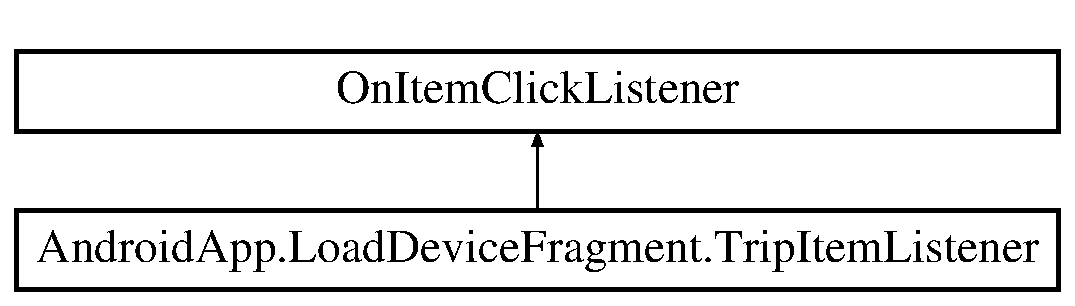
\includegraphics[height=2.000000cm]{class_android_app_1_1_load_device_fragment_1_1_trip_item_listener}
\end{center}
\end{figure}
\subsection*{Public Member Functions}
\begin{DoxyCompactItemize}
\item 
void \hyperlink{class_android_app_1_1_load_device_fragment_1_1_trip_item_listener_aa1eb00603eba3dbff13f1fa15bb9b958}{on\+Item\+Click} (Adapter\+View$<$?$>$ parent, View view, int position, long id)
\begin{DoxyCompactList}\small\item\em Loads a trip the user has specified. \end{DoxyCompactList}\end{DoxyCompactItemize}


\subsection{Detailed Description}
Listener used to identify when a trip has been pressed. 

\subsection{Member Function Documentation}
\mbox{\Hypertarget{class_android_app_1_1_load_device_fragment_1_1_trip_item_listener_aa1eb00603eba3dbff13f1fa15bb9b958}\label{class_android_app_1_1_load_device_fragment_1_1_trip_item_listener_aa1eb00603eba3dbff13f1fa15bb9b958}} 
\index{Android\+App\+::\+Load\+Device\+Fragment\+::\+Trip\+Item\+Listener@{Android\+App\+::\+Load\+Device\+Fragment\+::\+Trip\+Item\+Listener}!on\+Item\+Click@{on\+Item\+Click}}
\index{on\+Item\+Click@{on\+Item\+Click}!Android\+App\+::\+Load\+Device\+Fragment\+::\+Trip\+Item\+Listener@{Android\+App\+::\+Load\+Device\+Fragment\+::\+Trip\+Item\+Listener}}
\subsubsection{\texorpdfstring{on\+Item\+Click()}{onItemClick()}}
{\footnotesize\ttfamily void Android\+App.\+Load\+Device\+Fragment.\+Trip\+Item\+Listener.\+on\+Item\+Click (\begin{DoxyParamCaption}\item[{Adapter\+View$<$?$>$}]{parent,  }\item[{View}]{view,  }\item[{int}]{position,  }\item[{long}]{id }\end{DoxyParamCaption})\hspace{0.3cm}{\ttfamily [inline]}}



Loads a trip the user has specified. 

User has selected a trip via the List\+View, method switches to the statistic fragment and sends a message to logging device to load the specified trip (via name). 

References Android\+App.\+Trip\+Item.\+get\+Trip\+Name(), Android\+App.\+B\+T\+Connection.\+is\+Connected(), Android\+App.\+Realtime\+Fragment.\+R\+X\+Handler, Android\+App.\+B\+T\+Connection.\+set\+R\+X\+Handler(), and Android\+App.\+B\+T\+Connection.\+tx\+Handler.


\begin{DoxyCode}
138                                                                                          \{
139 
140             \textcolor{keywordflow}{if} (\hyperlink{class_android_app_1_1_load_device_fragment_a245147c7d3683cf1556680a382f328a9}{btConnection} != null && \hyperlink{class_android_app_1_1_load_device_fragment_a245147c7d3683cf1556680a382f328a9}{btConnection}.
      \hyperlink{class_android_app_1_1_b_t_connection_a1c91fcddfe9f3b69cd0141742103191a}{isConnected}()) \{
141                 TripItem tripItem = (TripItem) parent.getItemAtPosition(position);
142 
143                 \textcolor{comment}{/*}
144 \textcolor{comment}{                 * Create a new statistics fragment.}
145 \textcolor{comment}{                 * This will receive the stored data from the logging device.}
146 \textcolor{comment}{                 */}
147                 RealtimeFragment statFragment = \textcolor{keyword}{new} RealtimeFragment();
148                 \hyperlink{class_android_app_1_1_load_device_fragment_a245147c7d3683cf1556680a382f328a9}{btConnection}.\hyperlink{class_android_app_1_1_b_t_connection_a41022747db3c5a8bf0f4ddbc7bf32a3d}{setRXHandler}(statFragment.RXHandler);
149 
150                 \textcolor{comment}{/* Transmit over the name of the trip we want to load */}
151                 Message message = \textcolor{keyword}{new} Message();
152                 message.obj = (String) \hyperlink{class_android_app_1_1_load_device_fragment_afdfe423809d2267938f21eb4c5501653}{LOAD\_TRIP\_CHAR} + tripItem.getTripName();
153                 message.setTarget(\hyperlink{class_android_app_1_1_load_device_fragment_a245147c7d3683cf1556680a382f328a9}{btConnection}.\hyperlink{class_android_app_1_1_b_t_connection_a3236a74297d91f15dd63efc66f03a821}{txHandler});
154                 message.sendToTarget();
155 
156                 FragmentManager fragmentManager = getFragmentManager();
157                 fragmentManager.beginTransaction()
158                         .replace(R.id.content\_frame, statFragment)
159                         .commit();
160             \}
161         \}
\end{DoxyCode}


The documentation for this class was generated from the following file\+:\begin{DoxyCompactItemize}
\item 
android-\/app/app/src/main/java/com/jack/motorbikestatistics/\hyperlink{_load_device_fragment_8java}{Load\+Device\+Fragment.\+java}\end{DoxyCompactItemize}

\hypertarget{class_android_app_1_1_main_activity}{}\section{Android\+App.\+Main\+Activity Class Reference}
\label{class_android_app_1_1_main_activity}\index{Android\+App.\+Main\+Activity@{Android\+App.\+Main\+Activity}}


Main activity class for fragment navigation.  


Inheritance diagram for Android\+App.\+Main\+Activity\+:\begin{figure}[H]
\begin{center}
\leavevmode
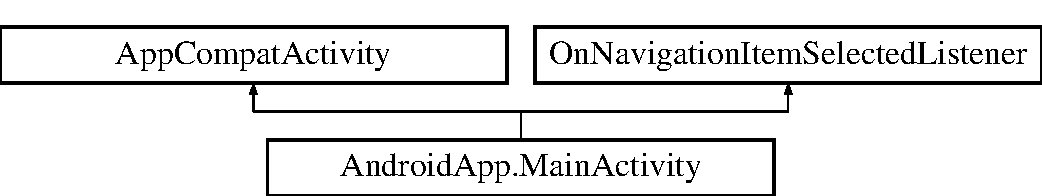
\includegraphics[height=2.000000cm]{class_android_app_1_1_main_activity}
\end{center}
\end{figure}
\subsection*{Public Member Functions}
\begin{DoxyCompactItemize}
\item 
\mbox{\Hypertarget{class_android_app_1_1_main_activity_afe0a73fb9e8d588b51f2cc8222da80e8}\label{class_android_app_1_1_main_activity_afe0a73fb9e8d588b51f2cc8222da80e8}} 
void \hyperlink{class_android_app_1_1_main_activity_afe0a73fb9e8d588b51f2cc8222da80e8}{on\+Back\+Pressed} ()
\begin{DoxyCompactList}\small\item\em Responsible for closing navigation drawer when back button pressed. \end{DoxyCompactList}\item 
boolean \hyperlink{class_android_app_1_1_main_activity_a260151867f535b62a2a926c270a2dbb8}{on\+Navigation\+Item\+Selected} (Menu\+Item item)
\begin{DoxyCompactList}\small\item\em Changes active fragment when a tab has been pressed. \end{DoxyCompactList}\end{DoxyCompactItemize}
\subsection*{Protected Member Functions}
\begin{DoxyCompactItemize}
\item 
void \hyperlink{class_android_app_1_1_main_activity_a2b1390dea8035d3802067ceb6ba5ebbd}{on\+Create} (Bundle saved\+Instance\+State)
\begin{DoxyCompactList}\small\item\em Function called when main activity is loaded. \end{DoxyCompactList}\end{DoxyCompactItemize}
\subsection*{Static Private Attributes}
\begin{DoxyCompactItemize}
\item 
\mbox{\Hypertarget{class_android_app_1_1_main_activity_a5b01be4fe68777c22779415e54432a79}\label{class_android_app_1_1_main_activity_a5b01be4fe68777c22779415e54432a79}} 
static final String \hyperlink{class_android_app_1_1_main_activity_a5b01be4fe68777c22779415e54432a79}{R\+E\+A\+L\+T\+I\+M\+E\+\_\+\+C\+H\+AR} = \char`\"{}1\char`\"{}
\begin{DoxyCompactList}\small\item\em Command for switching to realtime logging. \end{DoxyCompactList}\item 
\mbox{\Hypertarget{class_android_app_1_1_main_activity_a559f123628c037642baa46b37f23f5cc}\label{class_android_app_1_1_main_activity_a559f123628c037642baa46b37f23f5cc}} 
static final String \hyperlink{class_android_app_1_1_main_activity_a559f123628c037642baa46b37f23f5cc}{L\+I\+S\+T\+\_\+\+S\+A\+V\+E\+D\+\_\+\+C\+H\+AR} = \char`\"{}2\char`\"{}
\begin{DoxyCompactList}\small\item\em Command for loading all saved trip details. \end{DoxyCompactList}\item 
\mbox{\Hypertarget{class_android_app_1_1_main_activity_ad0c2b20cf0204ef3b8ad00596870e9a1}\label{class_android_app_1_1_main_activity_ad0c2b20cf0204ef3b8ad00596870e9a1}} 
static \hyperlink{class_android_app_1_1_realtime_fragment}{Realtime\+Fragment} \hyperlink{class_android_app_1_1_main_activity_ad0c2b20cf0204ef3b8ad00596870e9a1}{rt\+Fragment} = null
\begin{DoxyCompactList}\small\item\em UI fragment for realtime statistic display. \end{DoxyCompactList}\item 
\mbox{\Hypertarget{class_android_app_1_1_main_activity_ad54c7414ab4cb86c81e79f2f0037c694}\label{class_android_app_1_1_main_activity_ad54c7414ab4cb86c81e79f2f0037c694}} 
static \hyperlink{class_android_app_1_1_load_device_fragment}{Load\+Device\+Fragment} \hyperlink{class_android_app_1_1_main_activity_ad54c7414ab4cb86c81e79f2f0037c694}{ld\+Fragment} = null
\begin{DoxyCompactList}\small\item\em UI fragment for loading previous trips. \end{DoxyCompactList}\item 
\mbox{\Hypertarget{class_android_app_1_1_main_activity_a6dea684256a0cd0f73f87546ec2b0de2}\label{class_android_app_1_1_main_activity_a6dea684256a0cd0f73f87546ec2b0de2}} 
static \hyperlink{class_android_app_1_1_pair_device_fragment}{Pair\+Device\+Fragment} \hyperlink{class_android_app_1_1_main_activity_a6dea684256a0cd0f73f87546ec2b0de2}{pd\+Fragment} = null
\begin{DoxyCompactList}\small\item\em UI fragment for pairing to a logging device. \end{DoxyCompactList}\end{DoxyCompactItemize}


\subsection{Detailed Description}
Main activity class for fragment navigation. 

\subsection{Member Function Documentation}
\mbox{\Hypertarget{class_android_app_1_1_main_activity_a2b1390dea8035d3802067ceb6ba5ebbd}\label{class_android_app_1_1_main_activity_a2b1390dea8035d3802067ceb6ba5ebbd}} 
\index{Android\+App\+::\+Main\+Activity@{Android\+App\+::\+Main\+Activity}!on\+Create@{on\+Create}}
\index{on\+Create@{on\+Create}!Android\+App\+::\+Main\+Activity@{Android\+App\+::\+Main\+Activity}}
\subsubsection{\texorpdfstring{on\+Create()}{onCreate()}}
{\footnotesize\ttfamily void Android\+App.\+Main\+Activity.\+on\+Create (\begin{DoxyParamCaption}\item[{Bundle}]{saved\+Instance\+State }\end{DoxyParamCaption})\hspace{0.3cm}{\ttfamily [inline]}, {\ttfamily [protected]}}



Function called when main activity is loaded. 

Procedure is called when application is first started, sets up UI and creates relevant fragments.


\begin{DoxyParams}{Parameters}
{\em saved\+Instance\+State} & -\/ Information holding last previous state. \\
\hline
\end{DoxyParams}

\begin{DoxyCode}
55                                                        \{
56         super.onCreate(savedInstanceState);
57         setContentView(R.layout.activity\_main);
58 
59         Toolbar toolbar = (Toolbar) findViewById(R.id.toolbar);
60         setSupportActionBar(toolbar);
61 
62         DrawerLayout drawer = (DrawerLayout) findViewById(R.id.drawer\_layout);
63         ActionBarDrawerToggle toggle = \textcolor{keyword}{new} ActionBarDrawerToggle(
64                 \textcolor{keyword}{this}, drawer, toolbar, R.string.navigation\_drawer\_open, R.string.navigation\_drawer\_close);
65         drawer.setDrawerListener(toggle);
66         toggle.syncState();
67 
68         NavigationView navigationView = (NavigationView) findViewById(R.id.nav\_view);
69         navigationView.setNavigationItemSelectedListener(\textcolor{keyword}{this});
70 
71         \textcolor{comment}{/* Create our fragments for different sections of UI */}
72         \hyperlink{class_android_app_1_1_main_activity_ad0c2b20cf0204ef3b8ad00596870e9a1}{rtFragment} = \textcolor{keyword}{new} RealtimeFragment();
73         \hyperlink{class_android_app_1_1_main_activity_ad54c7414ab4cb86c81e79f2f0037c694}{ldFragment} = \textcolor{keyword}{new} LoadDeviceFragment();
74         \hyperlink{class_android_app_1_1_main_activity_a6dea684256a0cd0f73f87546ec2b0de2}{pdFragment} = \textcolor{keyword}{new} PairDeviceFragment();
75     \}
\end{DoxyCode}
\mbox{\Hypertarget{class_android_app_1_1_main_activity_a260151867f535b62a2a926c270a2dbb8}\label{class_android_app_1_1_main_activity_a260151867f535b62a2a926c270a2dbb8}} 
\index{Android\+App\+::\+Main\+Activity@{Android\+App\+::\+Main\+Activity}!on\+Navigation\+Item\+Selected@{on\+Navigation\+Item\+Selected}}
\index{on\+Navigation\+Item\+Selected@{on\+Navigation\+Item\+Selected}!Android\+App\+::\+Main\+Activity@{Android\+App\+::\+Main\+Activity}}
\subsubsection{\texorpdfstring{on\+Navigation\+Item\+Selected()}{onNavigationItemSelected()}}
{\footnotesize\ttfamily boolean Android\+App.\+Main\+Activity.\+on\+Navigation\+Item\+Selected (\begin{DoxyParamCaption}\item[{Menu\+Item}]{item }\end{DoxyParamCaption})\hspace{0.3cm}{\ttfamily [inline]}}



Changes active fragment when a tab has been pressed. 

Responsible for changing to the new chosen fragment on the UI. Opening of realtime and loaddevice fragments not possible when not connected to the logging device.

Method also responsible for change system state machine on the logging device, this is done by transmitting command code.


\begin{DoxyParams}{Parameters}
{\em item} & -\/ New selected fragment/tab to display. \\
\hline
\end{DoxyParams}


References Android\+App.\+Pair\+Device\+Fragment.\+get\+B\+T\+Connection(), Android\+App.\+B\+T\+Connection.\+is\+Connected(), Android\+App.\+Load\+Device\+Fragment.\+R\+X\+Handler, Android\+App.\+Realtime\+Fragment.\+R\+X\+Handler, Android\+App.\+Load\+Device\+Fragment.\+set\+B\+T\+Connection(), Android\+App.\+B\+T\+Connection.\+set\+R\+X\+Handler(), and Android\+App.\+B\+T\+Connection.\+tx\+Handler.


\begin{DoxyCode}
105                                                            \{
106 
107         Fragment activeFragment = null;
108 
109         \textcolor{comment}{/* Handle navigation view clicks here */}
110         FragmentManager fragmentManager = getFragmentManager();
111         \textcolor{keywordtype}{int} \textcolor{keywordtype}{id} = item.getItemId();
112 
113         \textcolor{keywordflow}{switch} (\textcolor{keywordtype}{id}) \{
114             \textcolor{keywordflow}{case} R.id.nav\_realtime: \{
115                 \textcolor{comment}{/* Get our bluetooth connection from pairing fragment */}
116                 BTConnection btConn = \hyperlink{class_android_app_1_1_main_activity_a6dea684256a0cd0f73f87546ec2b0de2}{pdFragment}.\hyperlink{class_android_app_1_1_pair_device_fragment_ae68bfed66a421a3020a257cbc034e42d}{getBTConnection}();
117 
118                 \textcolor{keywordflow}{if} (btConn != null && btConn.isConnected()) \{
119                     \textcolor{comment}{/* We set our RX handler and also send our command to indicate mode change */}
120                     btConn.\hyperlink{class_android_app_1_1_b_t_connection_a41022747db3c5a8bf0f4ddbc7bf32a3d}{setRXHandler}(\hyperlink{class_android_app_1_1_main_activity_ad0c2b20cf0204ef3b8ad00596870e9a1}{rtFragment}.
      \hyperlink{class_android_app_1_1_realtime_fragment_a6497ae268ff103aecc48a4bae15059d7}{RXHandler});
121                     Message message = \textcolor{keyword}{new} Message();
122                     message.obj = (String) \hyperlink{class_android_app_1_1_main_activity_a5b01be4fe68777c22779415e54432a79}{REALTIME\_CHAR};
123                     message.setTarget(btConn.txHandler);
124                     message.sendToTarget();
125 
126                     \textcolor{comment}{/* Change to our new active fragment */}
127                     activeFragment = \hyperlink{class_android_app_1_1_main_activity_ad0c2b20cf0204ef3b8ad00596870e9a1}{rtFragment};
128                 \} \textcolor{keywordflow}{else} \{
129                     \textcolor{comment}{/* Indicate that we are not connected to device */}
130                     View rootView = findViewById(R.id.content\_main);
131                     Snackbar.make(rootView, \textcolor{stringliteral}{"Please connect to a device first."}, Snackbar.LENGTH\_LONG)
132                             .setAction(\textcolor{stringliteral}{"Action"}, null).show();
133                 \}
134                 \textcolor{keywordflow}{break};
135             \}
136 
137             \textcolor{keywordflow}{case} R.id.nav\_loaddevice: \{
138                 \textcolor{comment}{/* Get our bluetooth connection from pairing fragment */}
139                 BTConnection btConn = \hyperlink{class_android_app_1_1_main_activity_a6dea684256a0cd0f73f87546ec2b0de2}{pdFragment}.\hyperlink{class_android_app_1_1_pair_device_fragment_ae68bfed66a421a3020a257cbc034e42d}{getBTConnection}();
140 
141                 \textcolor{keywordflow}{if} (btConn != null && btConn.isConnected()) \{
142                     \textcolor{comment}{/* We set our RX handler and also send our command to indicate mode change */}
143                     \hyperlink{class_android_app_1_1_main_activity_ad54c7414ab4cb86c81e79f2f0037c694}{ldFragment}.\hyperlink{class_android_app_1_1_load_device_fragment_a77ce93090f6c8c6aac522e35bfe9d21b}{setBTConnection}(btConn);
144 
145                     btConn.setRXHandler(\hyperlink{class_android_app_1_1_main_activity_ad54c7414ab4cb86c81e79f2f0037c694}{ldFragment}.\hyperlink{class_android_app_1_1_load_device_fragment_ad37565ea5a5332faf0c6b12284ca4e6c}{RXHandler});
146                     Message message = \textcolor{keyword}{new} Message();
147                     message.obj = (String) \hyperlink{class_android_app_1_1_main_activity_a559f123628c037642baa46b37f23f5cc}{LIST\_SAVED\_CHAR};
148                     message.setTarget(btConn.txHandler);
149                     message.sendToTarget();
150 
151                     \textcolor{comment}{/* Change to our new active fragment */}
152                     activeFragment = \hyperlink{class_android_app_1_1_main_activity_ad54c7414ab4cb86c81e79f2f0037c694}{ldFragment};
153                 \} \textcolor{keywordflow}{else} \{
154                     \textcolor{comment}{/* Indicate that we are not connected to device */}
155                     View rootView = findViewById(R.id.content\_main);
156                     Snackbar.make(rootView, \textcolor{stringliteral}{"Please connect to a device first."}, Snackbar.LENGTH\_LONG)
157                             .setAction(\textcolor{stringliteral}{"Action"}, null).show();
158                 \}
159                 \textcolor{keywordflow}{break};
160             \}
161 
162             \textcolor{keywordflow}{case} R.id.nav\_pairdevice: \{
163                 activeFragment = \hyperlink{class_android_app_1_1_main_activity_a6dea684256a0cd0f73f87546ec2b0de2}{pdFragment};
164             \}
165 
166         \}
167 
168         \textcolor{keywordflow}{if} (activeFragment != null) \{
169             \textcolor{comment}{/* Replaces content frame with newly selected one */}
170             fragmentManager.beginTransaction()
171                     .replace(R.id.content\_frame, activeFragment)
172                     .commit();
173         \}
174 
175         DrawerLayout drawer = (DrawerLayout) findViewById(R.id.drawer\_layout);
176         drawer.closeDrawer(GravityCompat.START);
177         \textcolor{keywordflow}{return} (activeFragment != null);
178     \}
\end{DoxyCode}


The documentation for this class was generated from the following file\+:\begin{DoxyCompactItemize}
\item 
android-\/app/app/src/main/java/com/jack/motorbikestatistics/\hyperlink{_main_activity_8java}{Main\+Activity.\+java}\end{DoxyCompactItemize}

\hypertarget{class_android_app_1_1_maps_activity}{}\section{Android\+App.\+Maps\+Activity Class Reference}
\label{class_android_app_1_1_maps_activity}\index{Android\+App.\+Maps\+Activity@{Android\+App.\+Maps\+Activity}}


Maps activity class for displaying map data.  


Inheritance diagram for Android\+App.\+Maps\+Activity\+:\begin{figure}[H]
\begin{center}
\leavevmode
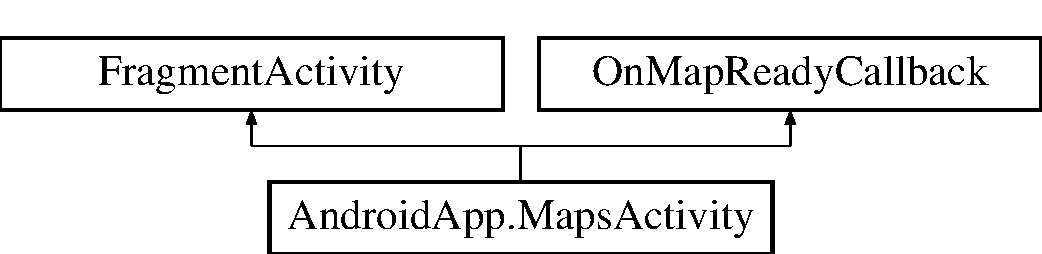
\includegraphics[height=2.000000cm]{class_android_app_1_1_maps_activity}
\end{center}
\end{figure}
\subsection*{Classes}
\begin{DoxyCompactItemize}
\item 
class \hyperlink{class_android_app_1_1_maps_activity_1_1_statistic_window_adapter}{Statistic\+Window\+Adapter}
\begin{DoxyCompactList}\small\item\em Adapter used for displaying statistics at a certain marker that user has clicked on. \end{DoxyCompactList}\item 
class \hyperlink{class_android_app_1_1_maps_activity_1_1_zoom_toogle_listener}{Zoom\+Toogle\+Listener}
\begin{DoxyCompactList}\small\item\em Listener class for making markers invisible when zoomed out. \end{DoxyCompactList}\end{DoxyCompactItemize}
\subsection*{Public Member Functions}
\begin{DoxyCompactItemize}
\item 
void \hyperlink{class_android_app_1_1_maps_activity_abee115dd67628da8e1140430428ce112}{on\+Map\+Ready} (Google\+Map google\+Map)
\begin{DoxyCompactList}\small\item\em Manipulates the map once available. \end{DoxyCompactList}\end{DoxyCompactItemize}
\subsection*{Protected Member Functions}
\begin{DoxyCompactItemize}
\item 
void \hyperlink{class_android_app_1_1_maps_activity_a179ec8e25e279c4fa33aa74a90019489}{on\+Create} (Bundle saved\+Instance\+State)
\begin{DoxyCompactList}\small\item\em Fills our maps array with points to plot on the map. \end{DoxyCompactList}\end{DoxyCompactItemize}
\subsection*{Private Member Functions}
\begin{DoxyCompactItemize}
\item 
J\+S\+O\+N\+Object \hyperlink{class_android_app_1_1_maps_activity_a18364d9334710362b1e6c39502353927}{find\+J\+S\+O\+N\+By\+Lat\+Lng} (Lat\+Lng position)
\begin{DoxyCompactList}\small\item\em Finds J\+S\+O\+N\+Object from Array\+List via L\+A\+T/\+L\+NG coordinates. \end{DoxyCompactList}\item 
float \hyperlink{class_android_app_1_1_maps_activity_aea9b9fe75f1d70e3c902c8348823efd0}{calc\+Distance} (Lat\+Lng start, Lat\+Lng end)
\begin{DoxyCompactList}\small\item\em Calculates the absolute distance between two points. \end{DoxyCompactList}\item 
float \hyperlink{class_android_app_1_1_maps_activity_a2f93b1f03094b96020cee7e06ce5fc85}{convert\+Dp\+To\+Pixel} (float dp, Context context)
\begin{DoxyCompactList}\small\item\em Function for converting raw DP value to pixels. \end{DoxyCompactList}\item 
Bitmap\+Descriptor \hyperlink{class_android_app_1_1_maps_activity_a77f66c756f18d56bd41f0ee1c889fb62}{get\+Bitmap\+Descriptor} (int id)
\begin{DoxyCompactList}\small\item\em Created a valid bitmap descriptor from a drawable resource ID. \end{DoxyCompactList}\end{DoxyCompactItemize}
\subsection*{Private Attributes}
\begin{DoxyCompactItemize}
\item 
\mbox{\Hypertarget{class_android_app_1_1_maps_activity_a373d4c770d2ab34538f9288d7c0e83ea}\label{class_android_app_1_1_maps_activity_a373d4c770d2ab34538f9288d7c0e83ea}} 
Google\+Map \hyperlink{class_android_app_1_1_maps_activity_a373d4c770d2ab34538f9288d7c0e83ea}{m\+Map}
\begin{DoxyCompactList}\small\item\em Google maps object for plotting. \end{DoxyCompactList}\item 
\mbox{\Hypertarget{class_android_app_1_1_maps_activity_ad2fa23bd9f7f5a501e91329413608528}\label{class_android_app_1_1_maps_activity_ad2fa23bd9f7f5a501e91329413608528}} 
Array\+List$<$ J\+S\+O\+N\+Object $>$ \hyperlink{class_android_app_1_1_maps_activity_ad2fa23bd9f7f5a501e91329413608528}{trip\+Data}
\begin{DoxyCompactList}\small\item\em Array\+List holding all trip data. \end{DoxyCompactList}\item 
\mbox{\Hypertarget{class_android_app_1_1_maps_activity_a85c831a59d0468fc03e695aa9beab77e}\label{class_android_app_1_1_maps_activity_a85c831a59d0468fc03e695aa9beab77e}} 
Array\+List$<$ Marker $>$ {\bfseries marker\+List}
\end{DoxyCompactItemize}


\subsection{Detailed Description}
Maps activity class for displaying map data. 

\subsection{Member Function Documentation}
\mbox{\Hypertarget{class_android_app_1_1_maps_activity_a179ec8e25e279c4fa33aa74a90019489}\label{class_android_app_1_1_maps_activity_a179ec8e25e279c4fa33aa74a90019489}} 
\index{Android\+App\+::\+Maps\+Activity@{Android\+App\+::\+Maps\+Activity}!on\+Create@{on\+Create}}
\index{on\+Create@{on\+Create}!Android\+App\+::\+Maps\+Activity@{Android\+App\+::\+Maps\+Activity}}
\subsubsection{\texorpdfstring{on\+Create()}{onCreate()}}
{\footnotesize\ttfamily void Android\+App.\+Maps\+Activity.\+on\+Create (\begin{DoxyParamCaption}\item[{Bundle}]{saved\+Instance\+State }\end{DoxyParamCaption})\hspace{0.3cm}{\ttfamily [inline]}, {\ttfamily [protected]}}



Fills our maps array with points to plot on the map. 

Called when maps activity is first started. Responsible for making sure we have points to plot.


\begin{DoxyParams}{Parameters}
{\em saved\+Instance\+State} & -\/ Information holding last previous state. \\
\hline
\end{DoxyParams}


References Android\+App.\+J\+S\+O\+N\+Handler\+Singleton.\+get\+Instance().


\begin{DoxyCode}
67                                                        \{
68         super.onCreate(savedInstanceState);
69         setContentView(R.layout.activity\_maps);
70         \textcolor{comment}{// Obtain the SupportMapFragment and get notified when the map is ready to be used.}
71         SupportMapFragment mapFragment = (SupportMapFragment) getSupportFragmentManager()
72                 .findFragmentById(R.id.map);
73 
74         \textcolor{comment}{/* Clear our marker list for new instances. */}
75         markerList = \textcolor{keyword}{new} ArrayList<Marker>();
76 
77         \textcolor{comment}{/* Get the tripData from our JSON handler singleton. */}
78         \hyperlink{class_android_app_1_1_maps_activity_ad2fa23bd9f7f5a501e91329413608528}{tripData} = JSONHandlerSingleton.getInstance().tripData;
79 
80         mapFragment.getMapAsync(\textcolor{keyword}{this});
81     \}
\end{DoxyCode}
\mbox{\Hypertarget{class_android_app_1_1_maps_activity_a18364d9334710362b1e6c39502353927}\label{class_android_app_1_1_maps_activity_a18364d9334710362b1e6c39502353927}} 
\index{Android\+App\+::\+Maps\+Activity@{Android\+App\+::\+Maps\+Activity}!find\+J\+S\+O\+N\+By\+Lat\+Lng@{find\+J\+S\+O\+N\+By\+Lat\+Lng}}
\index{find\+J\+S\+O\+N\+By\+Lat\+Lng@{find\+J\+S\+O\+N\+By\+Lat\+Lng}!Android\+App\+::\+Maps\+Activity@{Android\+App\+::\+Maps\+Activity}}
\subsubsection{\texorpdfstring{find\+J\+S\+O\+N\+By\+Lat\+Lng()}{findJSONByLatLng()}}
{\footnotesize\ttfamily J\+S\+O\+N\+Object Android\+App.\+Maps\+Activity.\+find\+J\+S\+O\+N\+By\+Lat\+Lng (\begin{DoxyParamCaption}\item[{Lat\+Lng}]{position }\end{DoxyParamCaption})\hspace{0.3cm}{\ttfamily [inline]}, {\ttfamily [private]}}



Finds J\+S\+O\+N\+Object from Array\+List via L\+A\+T/\+L\+NG coordinates. 


\begin{DoxyParams}{Parameters}
{\em position} & -\/ Latitude and Longitude position. \\
\hline
\end{DoxyParams}
\begin{DoxyReturn}{Returns}
J\+S\+O\+N\+Object -\/ The found J\+S\+ON object. 
\end{DoxyReturn}


References gps\+J\+S\+ON.


\begin{DoxyCode}
89                                                          \{
90         JSONObject result = null;
91 
92         \textcolor{keywordflow}{for} (\textcolor{keywordtype}{int} i = 0; i < \hyperlink{class_android_app_1_1_maps_activity_ad2fa23bd9f7f5a501e91329413608528}{tripData}.size(); i++) \{
93             JSONObject tmpJSON = \hyperlink{class_android_app_1_1_maps_activity_ad2fa23bd9f7f5a501e91329413608528}{tripData}.get(i);
94 
95             \textcolor{keywordflow}{try} \{
96                 JSONObject \hyperlink{logging-device_8ino_a548727e041a5cd3db91bdbd0ccd71e30}{gpsJSON} = tmpJSON.getJSONObject(\textcolor{stringliteral}{"gps"});
97 
98                 Double latitude = gpsJSON.getDouble(\textcolor{stringliteral}{"lat"});
99                 Double longitude = gpsJSON.getDouble(\textcolor{stringliteral}{"lng"});
100 
101                 \textcolor{comment}{/* Check to see if latitude and logitudes match */}
102                 \textcolor{keywordflow}{if} ((latitude == position.latitude) && (longitude == position.longitude)) \{
103                     result = tmpJSON;
104                     \textcolor{keywordflow}{break};
105                 \}
106 
107             \} \textcolor{keywordflow}{catch} (JSONException e) \{
108                 \textcolor{comment}{/* Do nothing */}
109             \}
110         \}
111 
112         \textcolor{keywordflow}{return} result;
113     \}
\end{DoxyCode}
\mbox{\Hypertarget{class_android_app_1_1_maps_activity_aea9b9fe75f1d70e3c902c8348823efd0}\label{class_android_app_1_1_maps_activity_aea9b9fe75f1d70e3c902c8348823efd0}} 
\index{Android\+App\+::\+Maps\+Activity@{Android\+App\+::\+Maps\+Activity}!calc\+Distance@{calc\+Distance}}
\index{calc\+Distance@{calc\+Distance}!Android\+App\+::\+Maps\+Activity@{Android\+App\+::\+Maps\+Activity}}
\subsubsection{\texorpdfstring{calc\+Distance()}{calcDistance()}}
{\footnotesize\ttfamily float Android\+App.\+Maps\+Activity.\+calc\+Distance (\begin{DoxyParamCaption}\item[{Lat\+Lng}]{start,  }\item[{Lat\+Lng}]{end }\end{DoxyParamCaption})\hspace{0.3cm}{\ttfamily [inline]}, {\ttfamily [private]}}



Calculates the absolute distance between two points. 

Distance is as the crow flys and not via streets etc. 
\begin{DoxyParams}{Parameters}
{\em start} & -\/ Start position. \\
\hline
{\em end} & -\/ End position. \\
\hline
\end{DoxyParams}
\begin{DoxyReturn}{Returns}
flaot -\/ Distance between points in metres. 
\end{DoxyReturn}

\begin{DoxyCode}
124     \{
125         \textcolor{keywordtype}{float}[] results = \textcolor{keyword}{new} \textcolor{keywordtype}{float}[1];
126 
127         Location.distanceBetween(start.latitude, start.longitude, end.latitude, end.longitude, results);
128         \textcolor{keywordflow}{return} results[0];
129     \}
\end{DoxyCode}
\mbox{\Hypertarget{class_android_app_1_1_maps_activity_abee115dd67628da8e1140430428ce112}\label{class_android_app_1_1_maps_activity_abee115dd67628da8e1140430428ce112}} 
\index{Android\+App\+::\+Maps\+Activity@{Android\+App\+::\+Maps\+Activity}!on\+Map\+Ready@{on\+Map\+Ready}}
\index{on\+Map\+Ready@{on\+Map\+Ready}!Android\+App\+::\+Maps\+Activity@{Android\+App\+::\+Maps\+Activity}}
\subsubsection{\texorpdfstring{on\+Map\+Ready()}{onMapReady()}}
{\footnotesize\ttfamily void Android\+App.\+Maps\+Activity.\+on\+Map\+Ready (\begin{DoxyParamCaption}\item[{Google\+Map}]{google\+Map }\end{DoxyParamCaption})\hspace{0.3cm}{\ttfamily [inline]}}



Manipulates the map once available. 

This callback is triggered when the map is ready to be used. This is where we can add markers or lines.

If Google Play services is not installed on the device, the user will be prompted to install it inside the Support\+Map\+Fragment. This method will only be triggered once the user has installed Google Play services and returned to the app.


\begin{DoxyParams}{Parameters}
{\em google\+Map} & -\/ Our map object ready to manipulate. \\
\hline
\end{DoxyParams}


References gps\+J\+S\+ON.


\begin{DoxyCode}
144                                                 \{
145         \hyperlink{class_android_app_1_1_maps_activity_a373d4c770d2ab34538f9288d7c0e83ea}{mMap} = googleMap;
146 
147         \hyperlink{class_android_app_1_1_maps_activity_a373d4c770d2ab34538f9288d7c0e83ea}{mMap}.setMapType(GoogleMap.MAP\_TYPE\_HYBRID);
148 
149         \textcolor{comment}{/* Set our info window adapter class that is shown when marker clicked */}
150         \hyperlink{class_android_app_1_1_maps_activity_a373d4c770d2ab34538f9288d7c0e83ea}{mMap}.setInfoWindowAdapter(\textcolor{keyword}{new} StatisticWindowAdapter());
151 
152         \textcolor{comment}{/* Set our listener class for adjusting visibility when zoomed. */}
153         \hyperlink{class_android_app_1_1_maps_activity_a373d4c770d2ab34538f9288d7c0e83ea}{mMap}.setOnCameraMoveListener(\textcolor{keyword}{new} ZoomToogleListener());
154 
155         \textcolor{comment}{/* If we have no data don't bother plotting points */}
156         \textcolor{keywordflow}{if} (\hyperlink{class_android_app_1_1_maps_activity_ad2fa23bd9f7f5a501e91329413608528}{tripData}.size() != 0)
157         \{
158             \textcolor{comment}{/* lineOpts will store our route */}
159             PolylineOptions lineOpts = \textcolor{keyword}{new} PolylineOptions();
160             lineOpts.color(Color.parseColor( \textcolor{stringliteral}{"#CCF44242"}));
161             lineOpts.width(18);
162             lineOpts.visible(\textcolor{keyword}{true});
163 
164             \textcolor{keywordflow}{try}
165             \{
166                 LatLng lastMarker = null;
167 
168                 \textcolor{comment}{/* Plot every point in the our JSONObject array */}
169                 \textcolor{keywordflow}{for} (\textcolor{keywordtype}{int} i = 0; i < \hyperlink{class_android_app_1_1_maps_activity_ad2fa23bd9f7f5a501e91329413608528}{tripData}.size(); i++)
170                 \{
171                     JSONObject rootJSON = \hyperlink{class_android_app_1_1_maps_activity_ad2fa23bd9f7f5a501e91329413608528}{tripData}.get(i);
172                     JSONObject \hyperlink{logging-device_8ino_a548727e041a5cd3db91bdbd0ccd71e30}{gpsJSON} = rootJSON.getJSONObject(\textcolor{stringliteral}{"gps"});
173 
174                     Double lat = gpsJSON.getDouble(\textcolor{stringliteral}{"lat"});
175                     Double lng = gpsJSON.getDouble(\textcolor{stringliteral}{"lng"});
176                     LatLng location = \textcolor{keyword}{new} LatLng(lat, lng);
177 
178                     \textcolor{comment}{/* Don't add location with invalid lat & lng. */}
179                     \textcolor{keywordflow}{if} (location.latitude != 0.00 && location.longitude != 0.00) \{
180 
181                         \textcolor{comment}{/* Add this location to our trip line */}
182                         lineOpts.add(location);
183 
184                         \textcolor{comment}{/*}
185 \textcolor{comment}{                         * Check if distance between this point and}
186 \textcolor{comment}{                         * last marker is greater than 5m otherwise don't add marker.}
187 \textcolor{comment}{                         * Adding markers every 5 metres prevents the map being spammed with}
188 \textcolor{comment}{                         * thousands of readings.}
189 \textcolor{comment}{                         */}
190                         \textcolor{keywordflow}{if} ((lastMarker == null) || (\hyperlink{class_android_app_1_1_maps_activity_aea9b9fe75f1d70e3c902c8348823efd0}{calcDistance}(location, lastMarker) > 5)) \{
191                             \textcolor{comment}{/* Only add a marker if the gps data is valid */}
192                             \textcolor{keywordflow}{if} (gpsJSON.getBoolean(\textcolor{stringliteral}{"gps\_valid"}) == \textcolor{keyword}{true}) \{
193                                 MarkerOptions markerOptions = \textcolor{keyword}{new} MarkerOptions();
194                                 markerOptions.position(location);
195                                 markerOptions.title(\textcolor{stringliteral}{"Reading: "} + i);
196                                 markerOptions.icon(\hyperlink{class_android_app_1_1_maps_activity_a77f66c756f18d56bd41f0ee1c889fb62}{getBitmapDescriptor}(R.drawable.
      ic\_expand\_more\_white\_24px));
197                                 markerOptions.visible(\textcolor{keyword}{false});
198 
199                                 \textcolor{comment}{/* Add our marker to map and to list. */}
200                                 markerList.add(\hyperlink{class_android_app_1_1_maps_activity_a373d4c770d2ab34538f9288d7c0e83ea}{mMap}.addMarker(markerOptions));
201 
202                                 lastMarker = location;
203 
204                                 \textcolor{comment}{/* Changes camera to point to newest marker */}
205                                 \hyperlink{class_android_app_1_1_maps_activity_a373d4c770d2ab34538f9288d7c0e83ea}{mMap}.animateCamera(CameraUpdateFactory.newLatLngZoom(location, 16));
206                             \}
207                         \}
208                     \}
209 
210                 \}
211                 \hyperlink{class_android_app_1_1_maps_activity_a373d4c770d2ab34538f9288d7c0e83ea}{mMap}.addPolyline(lineOpts);
212             \}
213             \textcolor{keywordflow}{catch} (JSONException e)
214             \{
215                 \textcolor{comment}{/* Do nothing */}
216             \}
217         \}
218     \}
\end{DoxyCode}
\mbox{\Hypertarget{class_android_app_1_1_maps_activity_a2f93b1f03094b96020cee7e06ce5fc85}\label{class_android_app_1_1_maps_activity_a2f93b1f03094b96020cee7e06ce5fc85}} 
\index{Android\+App\+::\+Maps\+Activity@{Android\+App\+::\+Maps\+Activity}!convert\+Dp\+To\+Pixel@{convert\+Dp\+To\+Pixel}}
\index{convert\+Dp\+To\+Pixel@{convert\+Dp\+To\+Pixel}!Android\+App\+::\+Maps\+Activity@{Android\+App\+::\+Maps\+Activity}}
\subsubsection{\texorpdfstring{convert\+Dp\+To\+Pixel()}{convertDpToPixel()}}
{\footnotesize\ttfamily float Android\+App.\+Maps\+Activity.\+convert\+Dp\+To\+Pixel (\begin{DoxyParamCaption}\item[{float}]{dp,  }\item[{Context}]{context }\end{DoxyParamCaption})\hspace{0.3cm}{\ttfamily [inline]}, {\ttfamily [private]}}



Function for converting raw DP value to pixels. 


\begin{DoxyParams}{Parameters}
{\em dp} & -\/ DP value. \\
\hline
{\em context} & -\/ Context of application. \\
\hline
\end{DoxyParams}
\begin{DoxyReturn}{Returns}
float -\/ Value in pixels. 
\end{DoxyReturn}

\begin{DoxyCode}
227                                                              \{
228         Resources resources = context.getResources();
229         DisplayMetrics metrics = resources.getDisplayMetrics();
230         \textcolor{keywordtype}{float} px = dp * ((float)metrics.densityDpi / DisplayMetrics.DENSITY\_DEFAULT);
231         \textcolor{keywordflow}{return} px;
232     \}
\end{DoxyCode}
\mbox{\Hypertarget{class_android_app_1_1_maps_activity_a77f66c756f18d56bd41f0ee1c889fb62}\label{class_android_app_1_1_maps_activity_a77f66c756f18d56bd41f0ee1c889fb62}} 
\index{Android\+App\+::\+Maps\+Activity@{Android\+App\+::\+Maps\+Activity}!get\+Bitmap\+Descriptor@{get\+Bitmap\+Descriptor}}
\index{get\+Bitmap\+Descriptor@{get\+Bitmap\+Descriptor}!Android\+App\+::\+Maps\+Activity@{Android\+App\+::\+Maps\+Activity}}
\subsubsection{\texorpdfstring{get\+Bitmap\+Descriptor()}{getBitmapDescriptor()}}
{\footnotesize\ttfamily Bitmap\+Descriptor Android\+App.\+Maps\+Activity.\+get\+Bitmap\+Descriptor (\begin{DoxyParamCaption}\item[{int}]{id }\end{DoxyParamCaption})\hspace{0.3cm}{\ttfamily [inline]}, {\ttfamily [private]}}



Created a valid bitmap descriptor from a drawable resource ID. 


\begin{DoxyParams}{Parameters}
{\em id} & -\/ Drawable resource ID. \\
\hline
\end{DoxyParams}
\begin{DoxyReturn}{Returns}
Bitmap\+Descriptor -\/ Bitmap image converted from Vector\+Asset. 
\end{DoxyReturn}

\begin{DoxyCode}
240                                                          \{
241 
242         Context context = getApplicationContext();
243         Drawable vectorDrawable = ContextCompat.getDrawable(context, \textcolor{keywordtype}{id});
244         \textcolor{keywordtype}{int} h = ((int) \hyperlink{class_android_app_1_1_maps_activity_a2f93b1f03094b96020cee7e06ce5fc85}{convertDpToPixel}(42, context));
245         \textcolor{keywordtype}{int} w = ((int) \hyperlink{class_android_app_1_1_maps_activity_a2f93b1f03094b96020cee7e06ce5fc85}{convertDpToPixel}(25, context));
246         vectorDrawable.setBounds(0, 0, w, h);
247         Bitmap bm = Bitmap.createBitmap(w, h, Bitmap.Config.ARGB\_8888);
248         Canvas canvas = \textcolor{keyword}{new} Canvas(bm);
249         vectorDrawable.draw(canvas);
250         \textcolor{keywordflow}{return} BitmapDescriptorFactory.fromBitmap(bm);
251     \}
\end{DoxyCode}


The documentation for this class was generated from the following file\+:\begin{DoxyCompactItemize}
\item 
android-\/app/app/src/main/java/com/jack/motorbikestatistics/\hyperlink{_maps_activity_8java}{Maps\+Activity.\+java}\end{DoxyCompactItemize}

\hypertarget{class_android_app_1_1_maps_activity_1_1_statistic_window_adapter}{}\section{Android\+App.\+Maps\+Activity.\+Statistic\+Window\+Adapter Class Reference}
\label{class_android_app_1_1_maps_activity_1_1_statistic_window_adapter}\index{Android\+App.\+Maps\+Activity.\+Statistic\+Window\+Adapter@{Android\+App.\+Maps\+Activity.\+Statistic\+Window\+Adapter}}


Adapter used for displaying statistics at a certain marker that user has clicked on.  


Inheritance diagram for Android\+App.\+Maps\+Activity.\+Statistic\+Window\+Adapter\+:\begin{figure}[H]
\begin{center}
\leavevmode
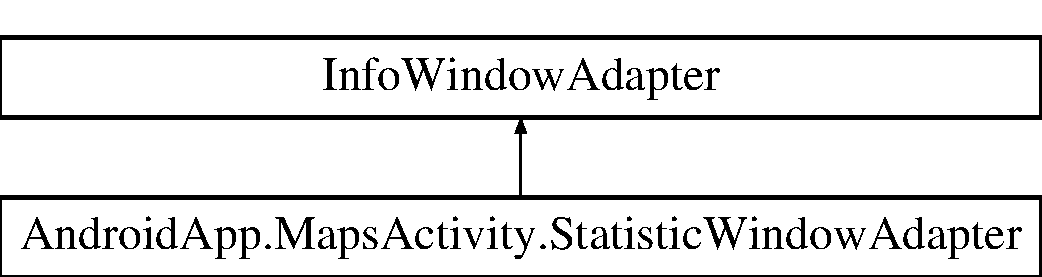
\includegraphics[height=2.000000cm]{class_android_app_1_1_maps_activity_1_1_statistic_window_adapter}
\end{center}
\end{figure}
\subsection*{Public Member Functions}
\begin{DoxyCompactItemize}
\item 
\mbox{\Hypertarget{class_android_app_1_1_maps_activity_1_1_statistic_window_adapter_a14860d57c39c0b2a3d2202aa9c416a59}\label{class_android_app_1_1_maps_activity_1_1_statistic_window_adapter_a14860d57c39c0b2a3d2202aa9c416a59}} 
View \hyperlink{class_android_app_1_1_maps_activity_1_1_statistic_window_adapter_a14860d57c39c0b2a3d2202aa9c416a59}{get\+Info\+Window} (Marker marker)
\begin{DoxyCompactList}\small\item\em We don\textquotesingle{}t want to use default information window. \end{DoxyCompactList}\item 
View \hyperlink{class_android_app_1_1_maps_activity_1_1_statistic_window_adapter_a19ae40ea5994ac2550ec599e3f20268b}{get\+Info\+Contents} (Marker marker)
\begin{DoxyCompactList}\small\item\em Displays statistics at a marker that the user has clicked on. \end{DoxyCompactList}\end{DoxyCompactItemize}


\subsection{Detailed Description}
Adapter used for displaying statistics at a certain marker that user has clicked on. 

\subsection{Member Function Documentation}
\mbox{\Hypertarget{class_android_app_1_1_maps_activity_1_1_statistic_window_adapter_a19ae40ea5994ac2550ec599e3f20268b}\label{class_android_app_1_1_maps_activity_1_1_statistic_window_adapter_a19ae40ea5994ac2550ec599e3f20268b}} 
\index{Android\+App\+::\+Maps\+Activity\+::\+Statistic\+Window\+Adapter@{Android\+App\+::\+Maps\+Activity\+::\+Statistic\+Window\+Adapter}!get\+Info\+Contents@{get\+Info\+Contents}}
\index{get\+Info\+Contents@{get\+Info\+Contents}!Android\+App\+::\+Maps\+Activity\+::\+Statistic\+Window\+Adapter@{Android\+App\+::\+Maps\+Activity\+::\+Statistic\+Window\+Adapter}}
\subsubsection{\texorpdfstring{get\+Info\+Contents()}{getInfoContents()}}
{\footnotesize\ttfamily View Android\+App.\+Maps\+Activity.\+Statistic\+Window\+Adapter.\+get\+Info\+Contents (\begin{DoxyParamCaption}\item[{Marker}]{marker }\end{DoxyParamCaption})\hspace{0.3cm}{\ttfamily [inline]}}



Displays statistics at a marker that the user has clicked on. 


\begin{DoxyParams}{Parameters}
{\em marker} & -\/ The marker the user has clicked on. \\
\hline
\end{DoxyParams}
\begin{DoxyReturn}{Returns}
View -\/ Updated view showing information. 
\end{DoxyReturn}


References gps\+J\+S\+ON, orient\+J\+S\+ON, and time\+J\+S\+ON.


\begin{DoxyCode}
254                                                    \{
255 
256             View v =  getLayoutInflater().inflate(R.layout.map\_marker\_info, null);
257 
258             \textcolor{comment}{/* Get latitude and longitude from marker */}
259             LatLng latlng = marker.getPosition();
260 
261             \textcolor{comment}{/* Find the JSONObject relating to this location */}
262             JSONObject rootJSON = \hyperlink{class_android_app_1_1_maps_activity_a18364d9334710362b1e6c39502353927}{findJSONByLatLng}(latlng);
263             \textcolor{keywordflow}{if} (rootJSON != null) \{
264                 \textcolor{keywordflow}{try} \{
265                     JSONObject \hyperlink{logging-device_8ino_a548727e041a5cd3db91bdbd0ccd71e30}{gpsJSON} = rootJSON.getJSONObject(\textcolor{stringliteral}{"gps"});
266                     JSONObject \hyperlink{logging-device_8ino_ae8e95a76df2aaa373792e5b744a6bb73}{orientJSON} = rootJSON.getJSONObject(\textcolor{stringliteral}{"orientation"});
267                     JSONObject \hyperlink{logging-device_8ino_acc172a29cb5ff709b48b650d9fb6503c}{timeJSON} = rootJSON.getJSONObject(\textcolor{stringliteral}{"time"});
268 
269                     \textcolor{comment}{/* Set latitude and longitude in info window */}
270                     TextView tvLatLng = (TextView)v.findViewById(R.id.map\_latlng);
271                     tvLatLng.setText(\textcolor{stringliteral}{"Lat/Lng: "} + Double.toString(latlng.latitude) + \textcolor{stringliteral}{"/"}
272                             + Double.toString(latlng.longitude));
273 
274                     \textcolor{comment}{/* Set time */}
275                     TextView tvTime = (TextView)v.findViewById(R.id.map\_time);
276                     Calendar cal = Calendar.getInstance();
277                     cal.clear();
278                     cal.set(Calendar.YEAR, timeJSON.getInt(\textcolor{stringliteral}{"year"}));
279                     cal.set(Calendar.MONTH, timeJSON.getInt(\textcolor{stringliteral}{"month"}));
280                     cal.set(Calendar.DATE, timeJSON.getInt(\textcolor{stringliteral}{"day"}));
281 
282                     cal.set(Calendar.HOUR, timeJSON.getInt(\textcolor{stringliteral}{"hour"}));
283                     cal.set(Calendar.MINUTE, timeJSON.getInt(\textcolor{stringliteral}{"minute"}));
284                     cal.set(Calendar.SECOND, timeJSON.getInt(\textcolor{stringliteral}{"second"}));
285                     cal.set(Calendar.MILLISECOND, timeJSON.getInt(\textcolor{stringliteral}{"centiseconds"}) * 10);
286 
287                     \textcolor{comment}{/* Create format for date and times then add to view */}
288                     DateFormat dateFormat = \textcolor{keyword}{new} SimpleDateFormat(\textcolor{stringliteral}{"dd/MM/yy HH:mm:ss.SS"});
289                     tvTime.setText(\textcolor{stringliteral}{"Time: "} + dateFormat.format(cal.getTime()));
290 
291                     \textcolor{comment}{/* Velocity & Altitude */}
292                     TextView tvVelocity = (TextView)v.findViewById(R.id.map\_velocity);
293                     tvVelocity.setText(\textcolor{stringliteral}{"Velocity: "} + gpsJSON.getDouble(\textcolor{stringliteral}{"vel\_mph"}) + \textcolor{stringliteral}{"mph"});
294 
295                     TextView tvAltitude = (TextView)v.findViewById(R.id.map\_altitude);
296                     tvAltitude.setText(\textcolor{stringliteral}{"Altitude: "} + gpsJSON.getDouble(\textcolor{stringliteral}{"alt\_ft"}) + \textcolor{stringliteral}{"ft"});
297 
298                     \textcolor{comment}{/* Orientation */}
299                     TextView tvPitch = (TextView)v.findViewById(R.id.map\_pitch);
300                     tvPitch.setText(\textcolor{stringliteral}{"Pitch Angle: "} + orientJSON.getDouble(\textcolor{stringliteral}{"pitch"}) + \textcolor{stringliteral}{"\(\backslash\)u00b0"});
301 
302                     TextView tvRoll = (TextView)v.findViewById(R.id.map\_roll);
303                     tvRoll.setText(\textcolor{stringliteral}{"Roll/Lean Angle: "} + orientJSON.getDouble(\textcolor{stringliteral}{"roll"}) + \textcolor{stringliteral}{"\(\backslash\)u00b0"});
304 
305                 \} \textcolor{keywordflow}{catch} (JSONException e) \{
306                     marker.hideInfoWindow();
307                 \}
308             \} \textcolor{keywordflow}{else} \{
309                 \textcolor{comment}{/* If unable to find relating we hide the info window */}
310                 marker.hideInfoWindow();
311             \}
312 
313             \textcolor{keywordflow}{return} v;
314         \}
\end{DoxyCode}


The documentation for this class was generated from the following file\+:\begin{DoxyCompactItemize}
\item 
android-\/app/app/src/main/java/com/jack/motorbikestatistics/\hyperlink{_maps_activity_8java}{Maps\+Activity.\+java}\end{DoxyCompactItemize}

\hypertarget{class_android_app_1_1_maps_activity_1_1_zoom_toogle_listener}{}\section{Android\+App.\+Maps\+Activity.\+Zoom\+Toogle\+Listener Class Reference}
\label{class_android_app_1_1_maps_activity_1_1_zoom_toogle_listener}\index{Android\+App.\+Maps\+Activity.\+Zoom\+Toogle\+Listener@{Android\+App.\+Maps\+Activity.\+Zoom\+Toogle\+Listener}}


Listener class for making markers invisible when zoomed out.  


Inheritance diagram for Android\+App.\+Maps\+Activity.\+Zoom\+Toogle\+Listener\+:\begin{figure}[H]
\begin{center}
\leavevmode
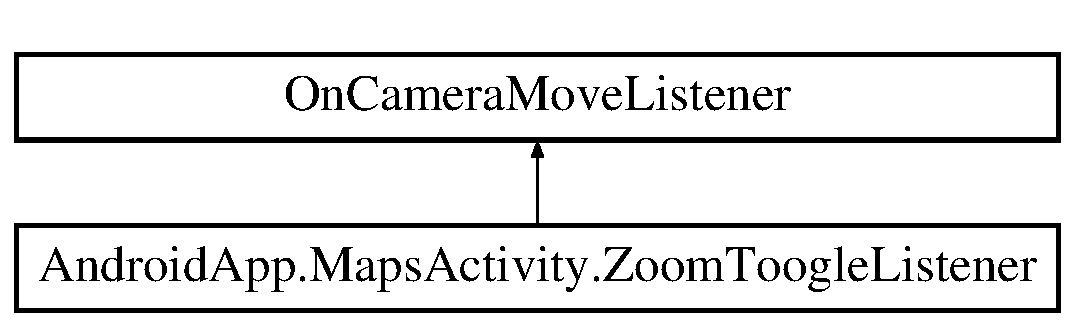
\includegraphics[height=2.000000cm]{class_android_app_1_1_maps_activity_1_1_zoom_toogle_listener}
\end{center}
\end{figure}
\subsection*{Public Member Functions}
\begin{DoxyCompactItemize}
\item 
\mbox{\Hypertarget{class_android_app_1_1_maps_activity_1_1_zoom_toogle_listener_ade815d6e8093f5020ac4676085f42669}\label{class_android_app_1_1_maps_activity_1_1_zoom_toogle_listener_ade815d6e8093f5020ac4676085f42669}} 
void \hyperlink{class_android_app_1_1_maps_activity_1_1_zoom_toogle_listener_ade815d6e8093f5020ac4676085f42669}{on\+Camera\+Move} ()
\begin{DoxyCompactList}\small\item\em Listener function that tooggles all markers visibility. \end{DoxyCompactList}\end{DoxyCompactItemize}
\subsection*{Private Member Functions}
\begin{DoxyCompactItemize}
\item 
void \hyperlink{class_android_app_1_1_maps_activity_1_1_zoom_toogle_listener_a87b5d78c37a7c1494cb84d613420286f}{set\+Markers\+Visible} (boolean visible)
\begin{DoxyCompactList}\small\item\em Sets all markers either visible or invisible. \end{DoxyCompactList}\end{DoxyCompactItemize}
\subsection*{Private Attributes}
\begin{DoxyCompactItemize}
\item 
\mbox{\Hypertarget{class_android_app_1_1_maps_activity_1_1_zoom_toogle_listener_a1c1bb0e72be3b6a370322a2b90518ab2}\label{class_android_app_1_1_maps_activity_1_1_zoom_toogle_listener_a1c1bb0e72be3b6a370322a2b90518ab2}} 
boolean {\bfseries current\+Visible} = false
\end{DoxyCompactItemize}


\subsection{Detailed Description}
Listener class for making markers invisible when zoomed out. 

\subsection{Member Function Documentation}
\mbox{\Hypertarget{class_android_app_1_1_maps_activity_1_1_zoom_toogle_listener_a87b5d78c37a7c1494cb84d613420286f}\label{class_android_app_1_1_maps_activity_1_1_zoom_toogle_listener_a87b5d78c37a7c1494cb84d613420286f}} 
\index{Android\+App\+::\+Maps\+Activity\+::\+Zoom\+Toogle\+Listener@{Android\+App\+::\+Maps\+Activity\+::\+Zoom\+Toogle\+Listener}!set\+Markers\+Visible@{set\+Markers\+Visible}}
\index{set\+Markers\+Visible@{set\+Markers\+Visible}!Android\+App\+::\+Maps\+Activity\+::\+Zoom\+Toogle\+Listener@{Android\+App\+::\+Maps\+Activity\+::\+Zoom\+Toogle\+Listener}}
\subsubsection{\texorpdfstring{set\+Markers\+Visible()}{setMarkersVisible()}}
{\footnotesize\ttfamily void Android\+App.\+Maps\+Activity.\+Zoom\+Toogle\+Listener.\+set\+Markers\+Visible (\begin{DoxyParamCaption}\item[{boolean}]{visible }\end{DoxyParamCaption})\hspace{0.3cm}{\ttfamily [inline]}, {\ttfamily [private]}}



Sets all markers either visible or invisible. 


\begin{DoxyParams}{Parameters}
{\em visible} & -\/ Value to set to. \\
\hline
\end{DoxyParams}

\begin{DoxyCode}
285                                                         \{
286             \textcolor{keywordflow}{if} (currentVisible != visible) \{
287                 \textcolor{keywordflow}{for} (\textcolor{keywordtype}{int} i = 0; i < markerList.size(); i++) \{
288 
289                     Marker tmp = markerList.get(i);
290                     tmp.setVisible(visible);
291                     currentVisible = visible;
292                 \}
293             \}
294         \}
\end{DoxyCode}


The documentation for this class was generated from the following file\+:\begin{DoxyCompactItemize}
\item 
android-\/app/app/src/main/java/com/jack/motorbikestatistics/\hyperlink{_maps_activity_8java}{Maps\+Activity.\+java}\end{DoxyCompactItemize}

\hypertarget{class_android_app_1_1_pair_device_fragment}{}\section{Android\+App.\+Pair\+Device\+Fragment Class Reference}
\label{class_android_app_1_1_pair_device_fragment}\index{Android\+App.\+Pair\+Device\+Fragment@{Android\+App.\+Pair\+Device\+Fragment}}


UI Class for discovering, pairing and connecting to the logging device.  


Inheritance diagram for Android\+App.\+Pair\+Device\+Fragment\+:\begin{figure}[H]
\begin{center}
\leavevmode
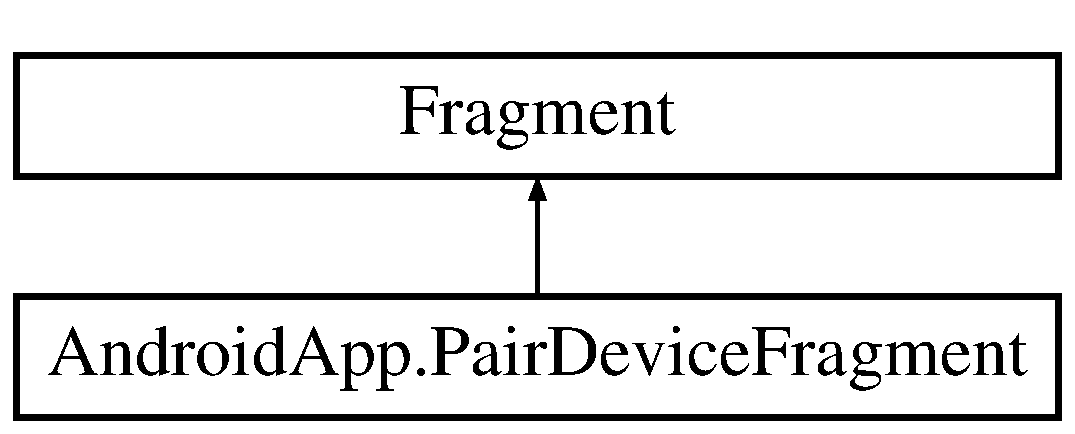
\includegraphics[height=2.000000cm]{class_android_app_1_1_pair_device_fragment}
\end{center}
\end{figure}
\subsection*{Classes}
\begin{DoxyCompactItemize}
\item 
class \hyperlink{class_android_app_1_1_pair_device_fragment_1_1_device_item_listener}{Device\+Item\+Listener}
\begin{DoxyCompactList}\small\item\em Listener for when a List\+View item is pressed (to connect). \end{DoxyCompactList}\item 
class \hyperlink{class_android_app_1_1_pair_device_fragment_1_1_discover_button_listener}{Discover\+Button\+Listener}
\begin{DoxyCompactList}\small\item\em Listener for when discovery button is pressed. \end{DoxyCompactList}\item 
class \hyperlink{class_android_app_1_1_pair_device_fragment_1_1_discover_receiver}{Discover\+Receiver}
\begin{DoxyCompactList}\small\item\em Receiver for when a new device is discovered. \end{DoxyCompactList}\end{DoxyCompactItemize}
\subsection*{Public Member Functions}
\begin{DoxyCompactItemize}
\item 
\hyperlink{class_android_app_1_1_pair_device_fragment_a0abb8db1228e66ff5073816588c77415}{Pair\+Device\+Fragment} ()
\begin{DoxyCompactList}\small\item\em Constructor for UI fragment. \end{DoxyCompactList}\item 
View \hyperlink{class_android_app_1_1_pair_device_fragment_af20a6287fc02c251141fef1c24b5e911}{on\+Create\+View} (Layout\+Inflater inflater, View\+Group container, Bundle saved\+Instance\+State)
\begin{DoxyCompactList}\small\item\em Function called when fragment is shown on UI. \end{DoxyCompactList}\item 
\hyperlink{class_android_app_1_1_b_t_connection}{B\+T\+Connection} \hyperlink{class_android_app_1_1_pair_device_fragment_ae68bfed66a421a3020a257cbc034e42d}{get\+B\+T\+Connection} ()
\begin{DoxyCompactList}\small\item\em Getter for getting current connected device. \end{DoxyCompactList}\end{DoxyCompactItemize}
\subsection*{Private Member Functions}
\begin{DoxyCompactItemize}
\item 
void \hyperlink{class_android_app_1_1_pair_device_fragment_ac6569d8f68c8023f2c2d38da55260f29}{get\+Needed\+Privileges} ()
\begin{DoxyCompactList}\small\item\em Prompts user for needed permissions of this application. \end{DoxyCompactList}\end{DoxyCompactItemize}
\subsection*{Private Attributes}
\begin{DoxyCompactItemize}
\item 
\mbox{\Hypertarget{class_android_app_1_1_pair_device_fragment_aab068c156fe3ef60bcb35328b697ba99}\label{class_android_app_1_1_pair_device_fragment_aab068c156fe3ef60bcb35328b697ba99}} 
boolean \hyperlink{class_android_app_1_1_pair_device_fragment_aab068c156fe3ef60bcb35328b697ba99}{first\+Run} = true
\begin{DoxyCompactList}\small\item\em Check variable used to stop List\+View from being re-\/populated. \end{DoxyCompactList}\item 
\mbox{\Hypertarget{class_android_app_1_1_pair_device_fragment_ada62059f31e97361bd94f2828cdc44e1}\label{class_android_app_1_1_pair_device_fragment_ada62059f31e97361bd94f2828cdc44e1}} 
Toggle\+Button \hyperlink{class_android_app_1_1_pair_device_fragment_ada62059f31e97361bd94f2828cdc44e1}{btn\+Scan}
\begin{DoxyCompactList}\small\item\em Scan button, used for toggling discovery. \end{DoxyCompactList}\item 
\mbox{\Hypertarget{class_android_app_1_1_pair_device_fragment_a54c71cf078647dbcd55742fc31a0a191}\label{class_android_app_1_1_pair_device_fragment_a54c71cf078647dbcd55742fc31a0a191}} 
Bluetooth\+Adapter \hyperlink{class_android_app_1_1_pair_device_fragment_a54c71cf078647dbcd55742fc31a0a191}{bt\+Adapter} = null
\begin{DoxyCompactList}\small\item\em Mobile\textquotesingle{}s bluetooth adapter. \end{DoxyCompactList}\item 
\mbox{\Hypertarget{class_android_app_1_1_pair_device_fragment_ac375aedac2d098332a1af1cf696f50a3}\label{class_android_app_1_1_pair_device_fragment_ac375aedac2d098332a1af1cf696f50a3}} 
Array\+List$<$ \hyperlink{class_android_app_1_1_b_t_device_item}{B\+T\+Device\+Item} $>$ \hyperlink{class_android_app_1_1_pair_device_fragment_ac375aedac2d098332a1af1cf696f50a3}{bt\+Device\+List}
\begin{DoxyCompactList}\small\item\em List of all devices, unpaired, paired \& connected. \end{DoxyCompactList}\item 
\mbox{\Hypertarget{class_android_app_1_1_pair_device_fragment_ab87b3da6318565e92d422a84685ab5b2}\label{class_android_app_1_1_pair_device_fragment_ab87b3da6318565e92d422a84685ab5b2}} 
Array\+List$<$ \hyperlink{class_android_app_1_1_b_t_device_item}{B\+T\+Device\+Item} $>$ \hyperlink{class_android_app_1_1_pair_device_fragment_ab87b3da6318565e92d422a84685ab5b2}{bt\+Paired\+List}
\begin{DoxyCompactList}\small\item\em List of only paired devices. \end{DoxyCompactList}\item 
\mbox{\Hypertarget{class_android_app_1_1_pair_device_fragment_a27eee15fc9f4328366bba7e795e026ac}\label{class_android_app_1_1_pair_device_fragment_a27eee15fc9f4328366bba7e795e026ac}} 
Array\+Adapter$<$ \hyperlink{class_android_app_1_1_b_t_device_item}{B\+T\+Device\+Item} $>$ \hyperlink{class_android_app_1_1_pair_device_fragment_a27eee15fc9f4328366bba7e795e026ac}{lv\+Adapter}
\begin{DoxyCompactList}\small\item\em UI adapter for List\+View that displays bluetooth devices. \end{DoxyCompactList}\item 
\mbox{\Hypertarget{class_android_app_1_1_pair_device_fragment_ac3d93a383672355ed54c56dc3e21e827}\label{class_android_app_1_1_pair_device_fragment_ac3d93a383672355ed54c56dc3e21e827}} 
\hyperlink{class_android_app_1_1_b_t_device_item}{B\+T\+Device\+Item} \hyperlink{class_android_app_1_1_pair_device_fragment_ac3d93a383672355ed54c56dc3e21e827}{bt\+Connected\+Device} = null
\begin{DoxyCompactList}\small\item\em Applications connected logging device. \end{DoxyCompactList}\item 
\mbox{\Hypertarget{class_android_app_1_1_pair_device_fragment_ada8ba66b955864829786ffcada7f5948}\label{class_android_app_1_1_pair_device_fragment_ada8ba66b955864829786ffcada7f5948}} 
\hyperlink{class_android_app_1_1_pair_device_fragment_1_1_discover_receiver}{Discover\+Receiver} \hyperlink{class_android_app_1_1_pair_device_fragment_ada8ba66b955864829786ffcada7f5948}{bt\+Receiver} = null
\begin{DoxyCompactList}\small\item\em Receiver class for when new device discovered. \end{DoxyCompactList}\end{DoxyCompactItemize}
\subsection*{Static Private Attributes}
\begin{DoxyCompactItemize}
\item 
\mbox{\Hypertarget{class_android_app_1_1_pair_device_fragment_a6d3f89529498ff90429ca5c74de2b177}\label{class_android_app_1_1_pair_device_fragment_a6d3f89529498ff90429ca5c74de2b177}} 
static final int \hyperlink{class_android_app_1_1_pair_device_fragment_a6d3f89529498ff90429ca5c74de2b177}{R\+E\+Q\+U\+E\+S\+T\+\_\+\+B\+L\+U\+E\+T\+O\+O\+TH} = 1
\begin{DoxyCompactList}\small\item\em Request code for activating bluetooth. \end{DoxyCompactList}\item 
\mbox{\Hypertarget{class_android_app_1_1_pair_device_fragment_a199a2a30c45008ec5a7360d11854f02f}\label{class_android_app_1_1_pair_device_fragment_a199a2a30c45008ec5a7360d11854f02f}} 
static final String \hyperlink{class_android_app_1_1_pair_device_fragment_a199a2a30c45008ec5a7360d11854f02f}{C\+O\+N\+N\+E\+C\+T\+E\+D\+\_\+\+S\+T\+A\+T\+US} = \char`\"{}connected\char`\"{}
\begin{DoxyCompactList}\small\item\em Status to change \hyperlink{class_android_app_1_1_b_t_device_item}{B\+T\+Device\+Item} to when connected. \end{DoxyCompactList}\item 
\mbox{\Hypertarget{class_android_app_1_1_pair_device_fragment_a68e4843e20a0d81574ba3d9e78a67be5}\label{class_android_app_1_1_pair_device_fragment_a68e4843e20a0d81574ba3d9e78a67be5}} 
static final int \hyperlink{class_android_app_1_1_pair_device_fragment_a68e4843e20a0d81574ba3d9e78a67be5}{B\+T\+\_\+\+D\+I\+S\+A\+B\+L\+E\+D\+\_\+\+I\+C\+ON} = R.\+drawable.\+ic\+\_\+bluetooth\+\_\+disabled\+\_\+black\+\_\+24px
\begin{DoxyCompactList}\small\item\em Icon ID to use when device is not connected. \end{DoxyCompactList}\end{DoxyCompactItemize}


\subsection{Detailed Description}
UI Class for discovering, pairing and connecting to the logging device. 

\subsection{Constructor \& Destructor Documentation}
\mbox{\Hypertarget{class_android_app_1_1_pair_device_fragment_a0abb8db1228e66ff5073816588c77415}\label{class_android_app_1_1_pair_device_fragment_a0abb8db1228e66ff5073816588c77415}} 
\index{Android\+App\+::\+Pair\+Device\+Fragment@{Android\+App\+::\+Pair\+Device\+Fragment}!Pair\+Device\+Fragment@{Pair\+Device\+Fragment}}
\index{Pair\+Device\+Fragment@{Pair\+Device\+Fragment}!Android\+App\+::\+Pair\+Device\+Fragment@{Android\+App\+::\+Pair\+Device\+Fragment}}
\subsubsection{\texorpdfstring{Pair\+Device\+Fragment()}{PairDeviceFragment()}}
{\footnotesize\ttfamily Android\+App.\+Pair\+Device\+Fragment.\+Pair\+Device\+Fragment (\begin{DoxyParamCaption}{ }\end{DoxyParamCaption})\hspace{0.3cm}{\ttfamily [inline]}}



Constructor for UI fragment. 

Get\textquotesingle{}s the mobile\textquotesingle{}s bluetooth adapter and sets up our lists of used for holding devices. 
\begin{DoxyCode}
85     \{
86         \textcolor{comment}{/* Get bluetooth adapter for device & create device arrays */}
87         \hyperlink{class_android_app_1_1_pair_device_fragment_a54c71cf078647dbcd55742fc31a0a191}{btAdapter} = BluetoothAdapter.getDefaultAdapter();
88         \hyperlink{class_android_app_1_1_pair_device_fragment_ac375aedac2d098332a1af1cf696f50a3}{btDeviceList} = \textcolor{keyword}{new} ArrayList<BTDeviceItem>();
89         \hyperlink{class_android_app_1_1_pair_device_fragment_ab87b3da6318565e92d422a84685ab5b2}{btPairedList} = \textcolor{keyword}{new} ArrayList<BTDeviceItem>();
90         \hyperlink{class_android_app_1_1_pair_device_fragment_ada8ba66b955864829786ffcada7f5948}{btReceiver} = \textcolor{keyword}{new} DiscoverReceiver();
91     \}
\end{DoxyCode}


\subsection{Member Function Documentation}
\mbox{\Hypertarget{class_android_app_1_1_pair_device_fragment_af20a6287fc02c251141fef1c24b5e911}\label{class_android_app_1_1_pair_device_fragment_af20a6287fc02c251141fef1c24b5e911}} 
\index{Android\+App\+::\+Pair\+Device\+Fragment@{Android\+App\+::\+Pair\+Device\+Fragment}!on\+Create\+View@{on\+Create\+View}}
\index{on\+Create\+View@{on\+Create\+View}!Android\+App\+::\+Pair\+Device\+Fragment@{Android\+App\+::\+Pair\+Device\+Fragment}}
\subsubsection{\texorpdfstring{on\+Create\+View()}{onCreateView()}}
{\footnotesize\ttfamily View Android\+App.\+Pair\+Device\+Fragment.\+on\+Create\+View (\begin{DoxyParamCaption}\item[{Layout\+Inflater}]{inflater,  }\item[{View\+Group}]{container,  }\item[{Bundle}]{saved\+Instance\+State }\end{DoxyParamCaption})\hspace{0.3cm}{\ttfamily [inline]}}



Function called when fragment is shown on UI. 

Sets up the UI List\+View and Buttons. Add all paired devices for the bluetooth adapter to the List\+View.


\begin{DoxyParams}{Parameters}
{\em inflater} & -\/ Inflater used for displaying view. \\
\hline
{\em container} & -\/ Container that the view will be displayed on. \\
\hline
{\em saved\+Instance\+State} & -\/ Last known state of this fragment. \\
\hline
\end{DoxyParams}
\begin{DoxyReturn}{Returns}
View -\/ The UI view of this fragment. 
\end{DoxyReturn}


References Android\+App.\+B\+T\+Device\+Item.\+get\+Connection(), Android\+App.\+B\+T\+Connection.\+is\+Connected(), and Android\+App.\+B\+T\+Connection.\+is\+Running().


\begin{DoxyCode}
106                                                                                                       \{
107 
108         View myView = inflater.inflate(R.layout.pairdevice\_layout, container, \textcolor{keyword}{false});
109 
110         \textcolor{comment}{/* Request needed privileges for bluetooth to work */}
111         \hyperlink{class_android_app_1_1_pair_device_fragment_ac6569d8f68c8023f2c2d38da55260f29}{getNeededPrivileges}();
112 
113         \textcolor{comment}{/* Set our variables for UI buttons */}
114         \hyperlink{class_android_app_1_1_pair_device_fragment_ada62059f31e97361bd94f2828cdc44e1}{btnScan} = (ToggleButton)myView.findViewById(R.id.pairdevice\_search);
115         \hyperlink{class_android_app_1_1_pair_device_fragment_ada62059f31e97361bd94f2828cdc44e1}{btnScan}.setOnCheckedChangeListener(\textcolor{keyword}{new} DiscoverButtonListener());
116 
117         ListView lvDevices = (ListView)myView.findViewById(R.id.pairdevice\_deviceList);
118         lvDevices.setOnItemClickListener(\textcolor{keyword}{new} DeviceItemListener());
119 
120         \hyperlink{class_android_app_1_1_pair_device_fragment_a27eee15fc9f4328366bba7e795e026ac}{lvAdapter} = \textcolor{keyword}{new} BTDeviceListAdapter(getActivity(), R.layout.device\_list\_item, 
      \hyperlink{class_android_app_1_1_pair_device_fragment_ac375aedac2d098332a1af1cf696f50a3}{btDeviceList});
121         lvDevices.setAdapter(\hyperlink{class_android_app_1_1_pair_device_fragment_a27eee15fc9f4328366bba7e795e026ac}{lvAdapter});
122 
123         \textcolor{comment}{/* Check and set up bluetooth adapter */}
124         \textcolor{keywordflow}{if} (\hyperlink{class_android_app_1_1_pair_device_fragment_a54c71cf078647dbcd55742fc31a0a191}{btAdapter} == null)
125         \{
126             Toast.makeText(getActivity().getApplicationContext(),
127                     \textcolor{stringliteral}{"This device has no bluetooth adapter"}, Toast.LENGTH\_LONG).show();
128         \}
129         \textcolor{keywordflow}{else}
130         \{
131             \textcolor{comment}{/* Check to see if connected device still is connected */}
132             \textcolor{keywordflow}{if} (\hyperlink{class_android_app_1_1_pair_device_fragment_ac3d93a383672355ed54c56dc3e21e827}{btConnectedDevice} != null)
133             \{
134                 \textcolor{keywordflow}{if} (!\hyperlink{class_android_app_1_1_pair_device_fragment_ac3d93a383672355ed54c56dc3e21e827}{btConnectedDevice}.\hyperlink{class_android_app_1_1_b_t_device_item_af256e53bf23dd3f969b14e0566a7b785}{getConnection}().
      \hyperlink{class_android_app_1_1_b_t_connection_a1c91fcddfe9f3b69cd0141742103191a}{isConnected}() ||
135                         !\hyperlink{class_android_app_1_1_pair_device_fragment_ac3d93a383672355ed54c56dc3e21e827}{btConnectedDevice}.\hyperlink{class_android_app_1_1_b_t_device_item_af256e53bf23dd3f969b14e0566a7b785}{getConnection}().
      \hyperlink{class_android_app_1_1_b_t_connection_a88abb39350aef278f15e54be4d0d1df3}{isRunning}())
136                 \{
137                     \hyperlink{class_android_app_1_1_pair_device_fragment_ac3d93a383672355ed54c56dc3e21e827}{btConnectedDevice} = null;
138                 \}
139             \}
140 
141             \textcolor{comment}{/* firstRun check to list from being re-populated */}
142             \textcolor{keywordflow}{if} (\hyperlink{class_android_app_1_1_pair_device_fragment_aab068c156fe3ef60bcb35328b697ba99}{firstRun})
143             \{
144                 \hyperlink{class_android_app_1_1_pair_device_fragment_aab068c156fe3ef60bcb35328b697ba99}{firstRun} = \textcolor{keyword}{false};
145 
146                 \textcolor{comment}{/* Enable bluetooth adapter if disabled */}
147                 \textcolor{keywordflow}{if} (!\hyperlink{class_android_app_1_1_pair_device_fragment_a54c71cf078647dbcd55742fc31a0a191}{btAdapter}.isEnabled())
148                 \{
149                     Intent enableBT = \textcolor{keyword}{new} Intent(BluetoothAdapter.ACTION\_REQUEST\_ENABLE);
150                     startActivityForResult(enableBT, \hyperlink{class_android_app_1_1_pair_device_fragment_a6d3f89529498ff90429ca5c74de2b177}{REQUEST\_BLUETOOTH});
151                 \}
152 
153                 \textcolor{keywordflow}{while} (!\hyperlink{class_android_app_1_1_pair_device_fragment_a54c71cf078647dbcd55742fc31a0a191}{btAdapter}.isEnabled())
154                 \{
155                     \textcolor{comment}{/* Wait for BT to be enabled */}
156                 \}
157 
158                 \textcolor{comment}{/* Add all paired devices to list */}
159                 Set<BluetoothDevice> pairedDevices = \hyperlink{class_android_app_1_1_pair_device_fragment_a54c71cf078647dbcd55742fc31a0a191}{btAdapter}.getBondedDevices();
160                 \textcolor{keywordflow}{if} (pairedDevices.size() > 0)
161                 \{
162                     \textcolor{keywordflow}{for} (BluetoothDevice device : pairedDevices)
163                     \{
164                         BTDeviceItem newDevice =
165                             \textcolor{keyword}{new} BTDeviceItem(device, \textcolor{stringliteral}{"paired"}, \hyperlink{class_android_app_1_1_pair_device_fragment_a68e4843e20a0d81574ba3d9e78a67be5}{BT\_DISABLED\_ICON});
166                         \hyperlink{class_android_app_1_1_pair_device_fragment_ab87b3da6318565e92d422a84685ab5b2}{btPairedList}.add(newDevice);
167                     \}
168                 \}
169                 \hyperlink{class_android_app_1_1_pair_device_fragment_ac375aedac2d098332a1af1cf696f50a3}{btDeviceList}.addAll(\hyperlink{class_android_app_1_1_pair_device_fragment_ab87b3da6318565e92d422a84685ab5b2}{btPairedList});
170             \}
171 
172         \}
173 
174         \textcolor{keywordflow}{return} myView;
175     \}
\end{DoxyCode}
\mbox{\Hypertarget{class_android_app_1_1_pair_device_fragment_ae68bfed66a421a3020a257cbc034e42d}\label{class_android_app_1_1_pair_device_fragment_ae68bfed66a421a3020a257cbc034e42d}} 
\index{Android\+App\+::\+Pair\+Device\+Fragment@{Android\+App\+::\+Pair\+Device\+Fragment}!get\+B\+T\+Connection@{get\+B\+T\+Connection}}
\index{get\+B\+T\+Connection@{get\+B\+T\+Connection}!Android\+App\+::\+Pair\+Device\+Fragment@{Android\+App\+::\+Pair\+Device\+Fragment}}
\subsubsection{\texorpdfstring{get\+B\+T\+Connection()}{getBTConnection()}}
{\footnotesize\ttfamily \hyperlink{class_android_app_1_1_b_t_connection}{B\+T\+Connection} Android\+App.\+Pair\+Device\+Fragment.\+get\+B\+T\+Connection (\begin{DoxyParamCaption}{ }\end{DoxyParamCaption})\hspace{0.3cm}{\ttfamily [inline]}}



Getter for getting current connected device. 

\begin{DoxyReturn}{Returns}
\hyperlink{class_android_app_1_1_b_t_connection}{B\+T\+Connection} -\/ Bluetooth device (logging device). 
\end{DoxyReturn}


References Android\+App.\+B\+T\+Device\+Item.\+get\+Connection().


\begin{DoxyCode}
182     \{
183         \textcolor{keywordflow}{if} (\hyperlink{class_android_app_1_1_pair_device_fragment_ac3d93a383672355ed54c56dc3e21e827}{btConnectedDevice} != null) \{
184             \textcolor{keywordflow}{return} \hyperlink{class_android_app_1_1_pair_device_fragment_ac3d93a383672355ed54c56dc3e21e827}{btConnectedDevice}.\hyperlink{class_android_app_1_1_b_t_device_item_af256e53bf23dd3f969b14e0566a7b785}{getConnection}();
185         \} \textcolor{keywordflow}{else} \{
186             \textcolor{keywordflow}{return} null;
187         \}
188     \}
\end{DoxyCode}
\mbox{\Hypertarget{class_android_app_1_1_pair_device_fragment_ac6569d8f68c8023f2c2d38da55260f29}\label{class_android_app_1_1_pair_device_fragment_ac6569d8f68c8023f2c2d38da55260f29}} 
\index{Android\+App\+::\+Pair\+Device\+Fragment@{Android\+App\+::\+Pair\+Device\+Fragment}!get\+Needed\+Privileges@{get\+Needed\+Privileges}}
\index{get\+Needed\+Privileges@{get\+Needed\+Privileges}!Android\+App\+::\+Pair\+Device\+Fragment@{Android\+App\+::\+Pair\+Device\+Fragment}}
\subsubsection{\texorpdfstring{get\+Needed\+Privileges()}{getNeededPrivileges()}}
{\footnotesize\ttfamily void Android\+App.\+Pair\+Device\+Fragment.\+get\+Needed\+Privileges (\begin{DoxyParamCaption}{ }\end{DoxyParamCaption})\hspace{0.3cm}{\ttfamily [inline]}, {\ttfamily [private]}}



Prompts user for needed permissions of this application. 

Due to android using a permissions/access method this method parses through each permission needed and prompts the user to accept. 
\begin{DoxyCode}
197     \{
198         \textcolor{keyword}{final} \textcolor{keywordtype}{int} REQUEST\_CODE = 5;
199 
200         \textcolor{keywordtype}{boolean} permsGranted = \textcolor{keyword}{true};
201         String[] permsToRequest =
202                 \{
203                         Manifest.permission.BLUETOOTH\_ADMIN,
204                         Manifest.permission.BLUETOOTH,
205                         Manifest.permission.ACCESS\_FINE\_LOCATION,
206                         Manifest.permission.ACCESS\_COARSE\_LOCATION
207                 \};
208 
209         \textcolor{keywordflow}{for} (String permission: permsToRequest)
210         \{
211             permsGranted &= (ContextCompat.checkSelfPermission(getActivity(), permission) == PackageManager
      .PERMISSION\_GRANTED);
212         \}
213 
214         \textcolor{keywordflow}{if} (!permsGranted)
215         \{
216             ActivityCompat.requestPermissions(getActivity(), permsToRequest, REQUEST\_CODE);
217         \}
218     \}
\end{DoxyCode}


The documentation for this class was generated from the following file\+:\begin{DoxyCompactItemize}
\item 
android-\/app/app/src/main/java/com/jack/motorbikestatistics/\hyperlink{_pair_device_fragment_8java}{Pair\+Device\+Fragment.\+java}\end{DoxyCompactItemize}

\hypertarget{class_android_app_1_1_pair_device_fragment_1_1_device_item_listener}{}\section{Android\+App.\+Pair\+Device\+Fragment.\+Device\+Item\+Listener Class Reference}
\label{class_android_app_1_1_pair_device_fragment_1_1_device_item_listener}\index{Android\+App.\+Pair\+Device\+Fragment.\+Device\+Item\+Listener@{Android\+App.\+Pair\+Device\+Fragment.\+Device\+Item\+Listener}}


Listener for when a List\+View item is pressed (to connect).  


Inheritance diagram for Android\+App.\+Pair\+Device\+Fragment.\+Device\+Item\+Listener\+:\begin{figure}[H]
\begin{center}
\leavevmode
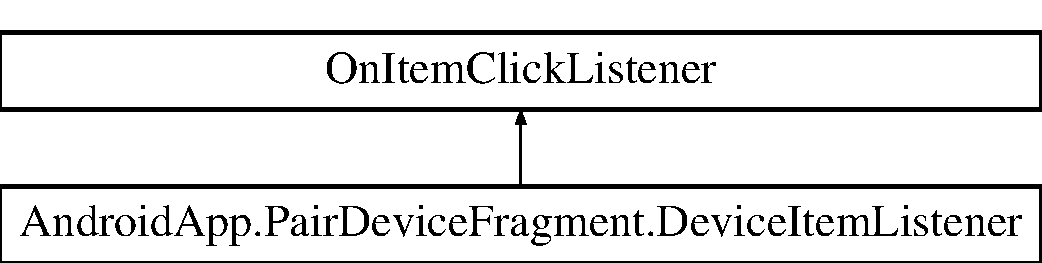
\includegraphics[height=2.000000cm]{class_android_app_1_1_pair_device_fragment_1_1_device_item_listener}
\end{center}
\end{figure}
\subsection*{Public Member Functions}
\begin{DoxyCompactItemize}
\item 
void \hyperlink{class_android_app_1_1_pair_device_fragment_1_1_device_item_listener_a6a396ee11bf3af843829045ccb7ffd5c}{on\+Item\+Click} (Adapter\+View$<$?$>$ parent, View view, int position, long id)
\begin{DoxyCompactList}\small\item\em Function called when user wants to connect to a device. \end{DoxyCompactList}\end{DoxyCompactItemize}


\subsection{Detailed Description}
Listener for when a List\+View item is pressed (to connect). 

\subsection{Member Function Documentation}
\mbox{\Hypertarget{class_android_app_1_1_pair_device_fragment_1_1_device_item_listener_a6a396ee11bf3af843829045ccb7ffd5c}\label{class_android_app_1_1_pair_device_fragment_1_1_device_item_listener_a6a396ee11bf3af843829045ccb7ffd5c}} 
\index{Android\+App\+::\+Pair\+Device\+Fragment\+::\+Device\+Item\+Listener@{Android\+App\+::\+Pair\+Device\+Fragment\+::\+Device\+Item\+Listener}!on\+Item\+Click@{on\+Item\+Click}}
\index{on\+Item\+Click@{on\+Item\+Click}!Android\+App\+::\+Pair\+Device\+Fragment\+::\+Device\+Item\+Listener@{Android\+App\+::\+Pair\+Device\+Fragment\+::\+Device\+Item\+Listener}}
\subsubsection{\texorpdfstring{on\+Item\+Click()}{onItemClick()}}
{\footnotesize\ttfamily void Android\+App.\+Pair\+Device\+Fragment.\+Device\+Item\+Listener.\+on\+Item\+Click (\begin{DoxyParamCaption}\item[{Adapter\+View$<$?$>$}]{parent,  }\item[{View}]{view,  }\item[{int}]{position,  }\item[{long}]{id }\end{DoxyParamCaption})\hspace{0.3cm}{\ttfamily [inline]}}



Function called when user wants to connect to a device. 

Discovery is turned off to stop power wastage. A new connection thread is then created which is responsible for parsing receive, and transmission requests from other fragments.


\begin{DoxyParams}{Parameters}
{\em parent} & -\/ The parent List\+View. \\
\hline
{\em view} & -\/ Current view of the List\+Item. \\
\hline
{\em position} & -\/ Index of item pressed in List\+View. \\
\hline
{\em id} & -\/ ID of the List\+Item. \\
\hline
\end{DoxyParams}


References Android\+App.\+B\+T\+Device\+Item.\+get\+Connection(), Android\+App.\+B\+T\+Device\+Item.\+get\+Device(), Android\+App.\+B\+T\+Connection.\+is\+Connected(), Android\+App.\+B\+T\+Device\+Item.\+set\+Connection(), Android\+App.\+B\+T\+Device\+Item.\+set\+Icon\+I\+D(), and Android\+App.\+B\+T\+Device\+Item.\+set\+Status().


\begin{DoxyCode}
305                                                                                          \{
306 
307             BTDeviceItem deviceItem = (BTDeviceItem)parent.getItemAtPosition(position);
308 
309             \textcolor{comment}{/* Check if there is already a connection between devices */}
310             \textcolor{keywordflow}{if} ((deviceItem.getConnection() == null) ||
311                     (!deviceItem.getConnection().isConnected()))
312             \{
313                 \textcolor{keywordflow}{if} (\hyperlink{class_android_app_1_1_pair_device_fragment_a54c71cf078647dbcd55742fc31a0a191}{btAdapter}.isDiscovering())
314                 \{
315                     \textcolor{comment}{/* Cancel discovery is still enabled */}
316                     \hyperlink{class_android_app_1_1_pair_device_fragment_ada62059f31e97361bd94f2828cdc44e1}{btnScan}.setChecked(\textcolor{keyword}{false});
317                     \hyperlink{class_android_app_1_1_pair_device_fragment_a54c71cf078647dbcd55742fc31a0a191}{btAdapter}.cancelDiscovery();
318                 \}
319 
320                 \textcolor{keywordflow}{try}
321                 \{
322                     Toast.makeText(parent.getContext(), \textcolor{stringliteral}{"Connecting to: "} +
323                             deviceItem.getDevice().getName(), Toast.LENGTH\_SHORT).show();
324 
325                     \textcolor{comment}{/* Create a new BTConnection item with no RX handler */}
326                     BTConnection newConn = \textcolor{keyword}{new} BTConnection(deviceItem.getDevice());
327 
328                     \textcolor{comment}{/* Execute the 'run' procedure in object in new thread */}
329                     Thread tmpThread = \textcolor{keyword}{new} Thread(newConn);
330                     tmpThread.start();
331 
332                     \textcolor{comment}{/* Add set connection and add item to listview */}
333                     deviceItem.setConnection(newConn);
334                     \hyperlink{class_android_app_1_1_pair_device_fragment_ac3d93a383672355ed54c56dc3e21e827}{btConnectedDevice} = deviceItem;
335 
336                     \textcolor{comment}{/* Update status and icon in list view */}
337                     deviceItem.\hyperlink{class_android_app_1_1_b_t_device_item_a893140b78c17184a199ac419f0fc7be7}{setIconID}(R.drawable.ic\_bluetooth\_connected\_black\_24px);
338                     deviceItem.setStatus(\hyperlink{class_android_app_1_1_pair_device_fragment_a199a2a30c45008ec5a7360d11854f02f}{CONNECTED\_STATUS});
339                     \hyperlink{class_android_app_1_1_pair_device_fragment_a27eee15fc9f4328366bba7e795e026ac}{lvAdapter}.notifyDataSetChanged();
340                 \}
341                 \textcolor{keywordflow}{catch} (IOException e)
342                 \{
343                     Toast.makeText(parent.getContext(), \textcolor{stringliteral}{"Unable to connect: "} +
344                             e.toString(), Toast.LENGTH\_SHORT).show();
345                 \}
346             \}
347         \}
\end{DoxyCode}


The documentation for this class was generated from the following file\+:\begin{DoxyCompactItemize}
\item 
android-\/app/app/src/main/java/com/jack/motorbikestatistics/\hyperlink{_pair_device_fragment_8java}{Pair\+Device\+Fragment.\+java}\end{DoxyCompactItemize}

\hypertarget{class_android_app_1_1_pair_device_fragment_1_1_discover_button_listener}{}\section{Android\+App.\+Pair\+Device\+Fragment.\+Discover\+Button\+Listener Class Reference}
\label{class_android_app_1_1_pair_device_fragment_1_1_discover_button_listener}\index{Android\+App.\+Pair\+Device\+Fragment.\+Discover\+Button\+Listener@{Android\+App.\+Pair\+Device\+Fragment.\+Discover\+Button\+Listener}}


Listener for when discovery button is pressed.  


Inheritance diagram for Android\+App.\+Pair\+Device\+Fragment.\+Discover\+Button\+Listener\+:\begin{figure}[H]
\begin{center}
\leavevmode
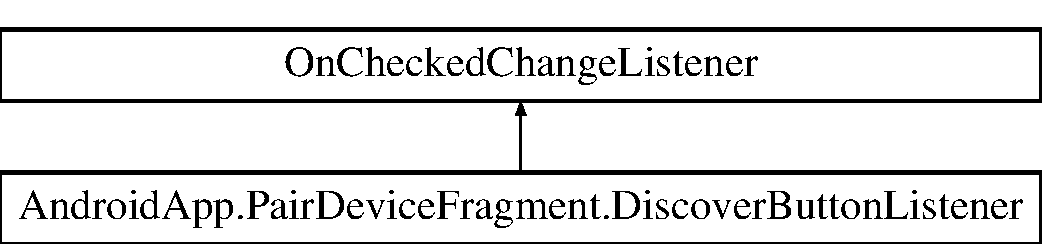
\includegraphics[height=2.000000cm]{class_android_app_1_1_pair_device_fragment_1_1_discover_button_listener}
\end{center}
\end{figure}
\subsection*{Public Member Functions}
\begin{DoxyCompactItemize}
\item 
void \hyperlink{class_android_app_1_1_pair_device_fragment_1_1_discover_button_listener_acda5197960ecaeaa1f98603e97a36bce}{on\+Checked\+Changed} (Compound\+Button button\+View, boolean is\+Checked)
\begin{DoxyCompactList}\small\item\em Function for handling when discover toggle button pressed. \end{DoxyCompactList}\end{DoxyCompactItemize}


\subsection{Detailed Description}
Listener for when discovery button is pressed. 

\subsection{Member Function Documentation}
\mbox{\Hypertarget{class_android_app_1_1_pair_device_fragment_1_1_discover_button_listener_acda5197960ecaeaa1f98603e97a36bce}\label{class_android_app_1_1_pair_device_fragment_1_1_discover_button_listener_acda5197960ecaeaa1f98603e97a36bce}} 
\index{Android\+App\+::\+Pair\+Device\+Fragment\+::\+Discover\+Button\+Listener@{Android\+App\+::\+Pair\+Device\+Fragment\+::\+Discover\+Button\+Listener}!on\+Checked\+Changed@{on\+Checked\+Changed}}
\index{on\+Checked\+Changed@{on\+Checked\+Changed}!Android\+App\+::\+Pair\+Device\+Fragment\+::\+Discover\+Button\+Listener@{Android\+App\+::\+Pair\+Device\+Fragment\+::\+Discover\+Button\+Listener}}
\subsubsection{\texorpdfstring{on\+Checked\+Changed()}{onCheckedChanged()}}
{\footnotesize\ttfamily void Android\+App.\+Pair\+Device\+Fragment.\+Discover\+Button\+Listener.\+on\+Checked\+Changed (\begin{DoxyParamCaption}\item[{Compound\+Button}]{button\+View,  }\item[{boolean}]{is\+Checked }\end{DoxyParamCaption})\hspace{0.3cm}{\ttfamily [inline]}}



Function for handling when discover toggle button pressed. 

If toggled on it bluetooth adapter is turned to discover mode. If toggled off bluetooth adapter is turn off of disover mode.


\begin{DoxyParams}{Parameters}
{\em button\+View} & -\/ Current view of the toggle button. \\
\hline
{\em is\+Checked} & -\/ The new state of the toggle button. \\
\hline
\end{DoxyParams}

\begin{DoxyCode}
262                                                                                    \{
263 
264             IntentFilter filter = \textcolor{keyword}{new} IntentFilter(BluetoothDevice.ACTION\_FOUND);
265             \textcolor{keywordflow}{if} (isChecked)
266             \{
267                 \textcolor{comment}{/* Clear listview, add previous paired items, start discovery */}
268                 \hyperlink{class_android_app_1_1_pair_device_fragment_a27eee15fc9f4328366bba7e795e026ac}{lvAdapter}.clear();
269                 \hyperlink{class_android_app_1_1_pair_device_fragment_a27eee15fc9f4328366bba7e795e026ac}{lvAdapter}.addAll(\hyperlink{class_android_app_1_1_pair_device_fragment_ab87b3da6318565e92d422a84685ab5b2}{btPairedList});
270 
271                 \textcolor{keywordflow}{if} (\hyperlink{class_android_app_1_1_pair_device_fragment_ac3d93a383672355ed54c56dc3e21e827}{btConnectedDevice} != null)
272                     \hyperlink{class_android_app_1_1_pair_device_fragment_a27eee15fc9f4328366bba7e795e026ac}{lvAdapter}.add(\hyperlink{class_android_app_1_1_pair_device_fragment_ac3d93a383672355ed54c56dc3e21e827}{btConnectedDevice});
273 
274                 getActivity().registerReceiver(\hyperlink{class_android_app_1_1_pair_device_fragment_ada8ba66b955864829786ffcada7f5948}{btReceiver}, filter);
275                 \hyperlink{class_android_app_1_1_pair_device_fragment_a54c71cf078647dbcd55742fc31a0a191}{btAdapter}.startDiscovery();
276             \}
277             \textcolor{keywordflow}{else}
278             \{
279                 \textcolor{comment}{/* Stop searching for new devices */}
280                 getActivity().unregisterReceiver(\hyperlink{class_android_app_1_1_pair_device_fragment_ada8ba66b955864829786ffcada7f5948}{btReceiver});
281                 \hyperlink{class_android_app_1_1_pair_device_fragment_a54c71cf078647dbcd55742fc31a0a191}{btAdapter}.cancelDiscovery();
282             \}
283         \}
\end{DoxyCode}


The documentation for this class was generated from the following file\+:\begin{DoxyCompactItemize}
\item 
android-\/app/app/src/main/java/com/jack/motorbikestatistics/\hyperlink{_pair_device_fragment_8java}{Pair\+Device\+Fragment.\+java}\end{DoxyCompactItemize}

\hypertarget{class_android_app_1_1_pair_device_fragment_1_1_discover_receiver}{}\section{Android\+App.\+Pair\+Device\+Fragment.\+Discover\+Receiver Class Reference}
\label{class_android_app_1_1_pair_device_fragment_1_1_discover_receiver}\index{Android\+App.\+Pair\+Device\+Fragment.\+Discover\+Receiver@{Android\+App.\+Pair\+Device\+Fragment.\+Discover\+Receiver}}


Receiver for when a new device is discovered.  


Inheritance diagram for Android\+App.\+Pair\+Device\+Fragment.\+Discover\+Receiver\+:\begin{figure}[H]
\begin{center}
\leavevmode
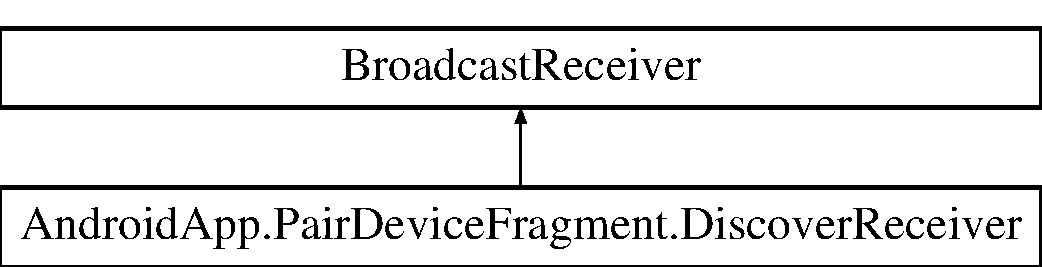
\includegraphics[height=2.000000cm]{class_android_app_1_1_pair_device_fragment_1_1_discover_receiver}
\end{center}
\end{figure}
\subsection*{Public Member Functions}
\begin{DoxyCompactItemize}
\item 
void \hyperlink{class_android_app_1_1_pair_device_fragment_1_1_discover_receiver_aed29343e83655c50dee0eb9253eb0b85}{on\+Receive} (Context context, Intent intent)
\begin{DoxyCompactList}\small\item\em When a BT device is found, adds the device to the List\+View. \end{DoxyCompactList}\end{DoxyCompactItemize}


\subsection{Detailed Description}
Receiver for when a new device is discovered. 

\subsection{Member Function Documentation}
\mbox{\Hypertarget{class_android_app_1_1_pair_device_fragment_1_1_discover_receiver_aed29343e83655c50dee0eb9253eb0b85}\label{class_android_app_1_1_pair_device_fragment_1_1_discover_receiver_aed29343e83655c50dee0eb9253eb0b85}} 
\index{Android\+App\+::\+Pair\+Device\+Fragment\+::\+Discover\+Receiver@{Android\+App\+::\+Pair\+Device\+Fragment\+::\+Discover\+Receiver}!on\+Receive@{on\+Receive}}
\index{on\+Receive@{on\+Receive}!Android\+App\+::\+Pair\+Device\+Fragment\+::\+Discover\+Receiver@{Android\+App\+::\+Pair\+Device\+Fragment\+::\+Discover\+Receiver}}
\subsubsection{\texorpdfstring{on\+Receive()}{onReceive()}}
{\footnotesize\ttfamily void Android\+App.\+Pair\+Device\+Fragment.\+Discover\+Receiver.\+on\+Receive (\begin{DoxyParamCaption}\item[{Context}]{context,  }\item[{Intent}]{intent }\end{DoxyParamCaption})\hspace{0.3cm}{\ttfamily [inline]}}



When a BT device is found, adds the device to the List\+View. 


\begin{DoxyParams}{Parameters}
{\em context} & -\/ Context that the application is running in. \\
\hline
{\em intent} & -\/ Intent holding the device object. \\
\hline
\end{DoxyParams}

\begin{DoxyCode}
231                                                               \{
232             String action = intent.getAction();
233 
234             \textcolor{comment}{/* Check to see if found device */}
235             \textcolor{keywordflow}{if} (BluetoothDevice.ACTION\_FOUND.equals(action))
236             \{
237                 BluetoothDevice device = intent.getParcelableExtra(BluetoothDevice.EXTRA\_DEVICE);
238 
239                 \textcolor{comment}{/* Create new device item and add to list */}
240                 BTDeviceItem newDevice = \textcolor{keyword}{new} BTDeviceItem(device, \textcolor{stringliteral}{"unpaired"}, 
      \hyperlink{class_android_app_1_1_pair_device_fragment_a68e4843e20a0d81574ba3d9e78a67be5}{BT\_DISABLED\_ICON});
241                 \hyperlink{class_android_app_1_1_pair_device_fragment_a27eee15fc9f4328366bba7e795e026ac}{lvAdapter}.add(newDevice);
242                 \hyperlink{class_android_app_1_1_pair_device_fragment_a27eee15fc9f4328366bba7e795e026ac}{lvAdapter}.notifyDataSetChanged();
243             \}
244         \}
\end{DoxyCode}


The documentation for this class was generated from the following file\+:\begin{DoxyCompactItemize}
\item 
android-\/app/app/src/main/java/com/jack/motorbikestatistics/\hyperlink{_pair_device_fragment_8java}{Pair\+Device\+Fragment.\+java}\end{DoxyCompactItemize}

\hypertarget{class_android_app_1_1_realtime_fragment}{}\section{Android\+App.\+Realtime\+Fragment Class Reference}
\label{class_android_app_1_1_realtime_fragment}\index{Android\+App.\+Realtime\+Fragment@{Android\+App.\+Realtime\+Fragment}}


UI Class for viewing data sent from the logging device.  


Inheritance diagram for Android\+App.\+Realtime\+Fragment\+:\begin{figure}[H]
\begin{center}
\leavevmode
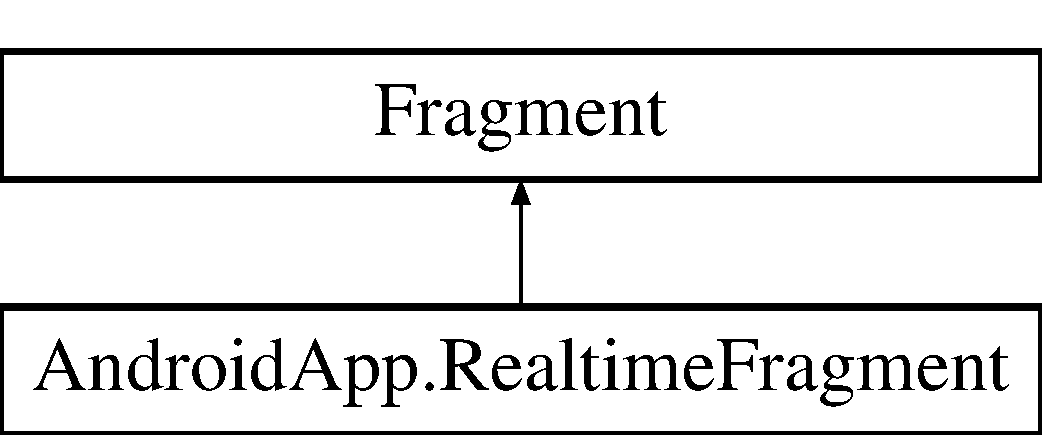
\includegraphics[height=2.000000cm]{class_android_app_1_1_realtime_fragment}
\end{center}
\end{figure}
\subsection*{Classes}
\begin{DoxyCompactItemize}
\item 
class \hyperlink{class_android_app_1_1_realtime_fragment_1_1_map_button_listener}{Map\+Button\+Listener}
\begin{DoxyCompactList}\small\item\em Listener for starting a map activity when button pressed. \end{DoxyCompactList}\end{DoxyCompactItemize}
\subsection*{Public Member Functions}
\begin{DoxyCompactItemize}
\item 
\hyperlink{class_android_app_1_1_realtime_fragment_a834ef524bedd8948892a6915945c071c}{Realtime\+Fragment} ()
\begin{DoxyCompactList}\small\item\em Constructor for UI fragment. \end{DoxyCompactList}\item 
View \hyperlink{class_android_app_1_1_realtime_fragment_a9efde75b84b4566f528b5cd53c908917}{on\+Create\+View} (Layout\+Inflater inflater, View\+Group container, Bundle saved\+Instance\+State)
\begin{DoxyCompactList}\small\item\em Function called when fragment is shown on UI. \end{DoxyCompactList}\end{DoxyCompactItemize}
\subsection*{Public Attributes}
\begin{DoxyCompactItemize}
\item 
final Handler \hyperlink{class_android_app_1_1_realtime_fragment_a6497ae268ff103aecc48a4bae15059d7}{R\+X\+Handler}
\begin{DoxyCompactList}\small\item\em Handler used for receiving statistics via bluetooth. \end{DoxyCompactList}\end{DoxyCompactItemize}
\subsection*{Private Member Functions}
\begin{DoxyCompactItemize}
\item 
final void \hyperlink{class_android_app_1_1_realtime_fragment_a61735e07c8f7b382b176d7cd7443de3f}{new\+Data} (J\+S\+O\+N\+Object json\+Data)
\begin{DoxyCompactList}\small\item\em Function for adding new statistics when received via bluetooth. \end{DoxyCompactList}\end{DoxyCompactItemize}
\subsection*{Private Attributes}
\begin{DoxyCompactItemize}
\item 
\mbox{\Hypertarget{class_android_app_1_1_realtime_fragment_a8aa6530bcc9c6ef17627f1395ff7910d}\label{class_android_app_1_1_realtime_fragment_a8aa6530bcc9c6ef17627f1395ff7910d}} 
Text\+View \hyperlink{class_android_app_1_1_realtime_fragment_a8aa6530bcc9c6ef17627f1395ff7910d}{text\+Status}
\begin{DoxyCompactList}\small\item\em Text\+View to show amount of logs received. \end{DoxyCompactList}\item 
\mbox{\Hypertarget{class_android_app_1_1_realtime_fragment_a4c3f12bcaaab715dc512d4cd4a4c11cf}\label{class_android_app_1_1_realtime_fragment_a4c3f12bcaaab715dc512d4cd4a4c11cf}} 
Array\+List$<$ String $>$ \hyperlink{class_android_app_1_1_realtime_fragment_a4c3f12bcaaab715dc512d4cd4a4c11cf}{json\+List}
\begin{DoxyCompactList}\small\item\em Array that holds serialised trip data to pass to map. \end{DoxyCompactList}\item 
\mbox{\Hypertarget{class_android_app_1_1_realtime_fragment_ab1c4983b61e50b501ed22842253bf849}\label{class_android_app_1_1_realtime_fragment_ab1c4983b61e50b501ed22842253bf849}} 
\hyperlink{class_android_app_1_1_set_of_data_items}{Set\+Of\+Data\+Items} \hyperlink{class_android_app_1_1_realtime_fragment_ab1c4983b61e50b501ed22842253bf849}{data\+List}
\begin{DoxyCompactList}\small\item\em Array holding each statistic that device is measuring. \end{DoxyCompactList}\item 
\mbox{\Hypertarget{class_android_app_1_1_realtime_fragment_afeafb95e85d8ba0b9c50aa36af2f4216}\label{class_android_app_1_1_realtime_fragment_afeafb95e85d8ba0b9c50aa36af2f4216}} 
Array\+Adapter$<$ \hyperlink{class_android_app_1_1_data_item}{Data\+Item} $>$ \hyperlink{class_android_app_1_1_realtime_fragment_afeafb95e85d8ba0b9c50aa36af2f4216}{lv\+Adapter}
\begin{DoxyCompactList}\small\item\em Adapter used for displaying statistics in the List\+View. \end{DoxyCompactList}\end{DoxyCompactItemize}
\subsection*{Static Private Attributes}
\begin{DoxyCompactItemize}
\item 
\mbox{\Hypertarget{class_android_app_1_1_realtime_fragment_a353558a83a489be25f413e3ea2451728}\label{class_android_app_1_1_realtime_fragment_a353558a83a489be25f413e3ea2451728}} 
static final String \hyperlink{class_android_app_1_1_realtime_fragment_a353558a83a489be25f413e3ea2451728}{N\+E\+W\+\_\+\+L\+I\+NE} = \char`\"{}\textbackslash{}r\textbackslash{}n\char`\"{}
\begin{DoxyCompactList}\small\item\em String for new line parsing. \end{DoxyCompactList}\end{DoxyCompactItemize}


\subsection{Detailed Description}
UI Class for viewing data sent from the logging device. 

\subsection{Constructor \& Destructor Documentation}
\mbox{\Hypertarget{class_android_app_1_1_realtime_fragment_a834ef524bedd8948892a6915945c071c}\label{class_android_app_1_1_realtime_fragment_a834ef524bedd8948892a6915945c071c}} 
\index{Android\+App\+::\+Realtime\+Fragment@{Android\+App\+::\+Realtime\+Fragment}!Realtime\+Fragment@{Realtime\+Fragment}}
\index{Realtime\+Fragment@{Realtime\+Fragment}!Android\+App\+::\+Realtime\+Fragment@{Android\+App\+::\+Realtime\+Fragment}}
\subsubsection{\texorpdfstring{Realtime\+Fragment()}{RealtimeFragment()}}
{\footnotesize\ttfamily Android\+App.\+Realtime\+Fragment.\+Realtime\+Fragment (\begin{DoxyParamCaption}{ }\end{DoxyParamCaption})\hspace{0.3cm}{\ttfamily [inline]}}



Constructor for UI fragment. 

Creates our initial data items that we are going to log. Setting whether extended functionality is needed for each data item. 
\begin{DoxyCode}
62                               \{
63         \hyperlink{class_android_app_1_1_realtime_fragment_a4c3f12bcaaab715dc512d4cd4a4c11cf}{jsonList} = \textcolor{keyword}{new} ArrayList<String>();
64 
65         \hyperlink{class_android_app_1_1_realtime_fragment_ab1c4983b61e50b501ed22842253bf849}{dataList} = \textcolor{keyword}{new} SetOfDataItems();
66 
67         \textcolor{comment}{/* Set up our data items that we will want to log */}
68         dataList.add(\textcolor{keyword}{new} DataItem<Double>(\textcolor{stringliteral}{"Yaw"}, \textcolor{keyword}{true}));
69         dataList.add(\textcolor{keyword}{new} DataItem<Double>(\textcolor{stringliteral}{"Pitch"}, \textcolor{keyword}{true}));
70         dataList.add(\textcolor{keyword}{new} DataItem<Double>(\textcolor{stringliteral}{"Roll"}, \textcolor{keyword}{true}));
71         dataList.add(\textcolor{keyword}{new} DataItem<Boolean>(\textcolor{stringliteral}{"GPS Valid"}, \textcolor{keyword}{false}));
72         dataList.add(\textcolor{keyword}{new} DataItem<Integer>(\textcolor{stringliteral}{"Satellites"}, \textcolor{keyword}{false}));
73         dataList.add(\textcolor{keyword}{new} DataItem<Double>(\textcolor{stringliteral}{"Latitude"}, \textcolor{keyword}{false}));
74         dataList.add(\textcolor{keyword}{new} DataItem<Double>(\textcolor{stringliteral}{"Longitude"}, \textcolor{keyword}{false}));
75         dataList.add(\textcolor{keyword}{new} DataItem<Double>(\textcolor{stringliteral}{"Velocity (MPH)"}, \textcolor{keyword}{true}));
76         dataList.add(\textcolor{keyword}{new} DataItem<Double>(\textcolor{stringliteral}{"Altitude (FT)"}, \textcolor{keyword}{true}));
77         dataList.add(\textcolor{keyword}{new} DataItem<Boolean>(\textcolor{stringliteral}{"Date Valid"}, \textcolor{keyword}{false}));
78         dataList.add(\textcolor{keyword}{new} DataItem<String>(\textcolor{stringliteral}{"Date"}, \textcolor{keyword}{false}));
79         dataList.add(\textcolor{keyword}{new} DataItem<String>(\textcolor{stringliteral}{"Time"}, \textcolor{keyword}{false}));
80     \}
\end{DoxyCode}


\subsection{Member Function Documentation}
\mbox{\Hypertarget{class_android_app_1_1_realtime_fragment_a9efde75b84b4566f528b5cd53c908917}\label{class_android_app_1_1_realtime_fragment_a9efde75b84b4566f528b5cd53c908917}} 
\index{Android\+App\+::\+Realtime\+Fragment@{Android\+App\+::\+Realtime\+Fragment}!on\+Create\+View@{on\+Create\+View}}
\index{on\+Create\+View@{on\+Create\+View}!Android\+App\+::\+Realtime\+Fragment@{Android\+App\+::\+Realtime\+Fragment}}
\subsubsection{\texorpdfstring{on\+Create\+View()}{onCreateView()}}
{\footnotesize\ttfamily View Android\+App.\+Realtime\+Fragment.\+on\+Create\+View (\begin{DoxyParamCaption}\item[{Layout\+Inflater}]{inflater,  }\item[{View\+Group}]{container,  }\item[{Bundle}]{saved\+Instance\+State }\end{DoxyParamCaption})\hspace{0.3cm}{\ttfamily [inline]}}



Function called when fragment is shown on UI. 

Sets up the UI List\+View and Buttons.


\begin{DoxyParams}{Parameters}
{\em inflater} & -\/ Inflater used for displaying view. \\
\hline
{\em container} & -\/ Container that the view will be displayed on. \\
\hline
{\em saved\+Instance\+State} & -\/ Last known state of this fragment. \\
\hline
\end{DoxyParams}
\begin{DoxyReturn}{Returns}
View -\/ The UI view of this fragment. 
\end{DoxyReturn}

\begin{DoxyCode}
94                                                                                                       \{
95         View myView = inflater.inflate(R.layout.realtime\_layout, container, \textcolor{keyword}{false});
96 
97         \hyperlink{class_android_app_1_1_realtime_fragment_a8aa6530bcc9c6ef17627f1395ff7910d}{textStatus} = (TextView)myView.findViewById(R.id.realtime\_status);
98 
99         \textcolor{comment}{/* Get the ListView via ID */}
100         ListView lvDataItems = (ListView) myView.findViewById(R.id.realtime\_data\_list);
101 
102         \textcolor{comment}{/* Inflate the header view for ListView */}
103         ViewGroup headerView = (ViewGroup) inflater.inflate(R.layout.data\_list\_header, lvDataItems, \textcolor{keyword}{false});
104         lvDataItems.addHeaderView(headerView);
105 
106         \textcolor{comment}{/* Create our new list adapter for our data list view */}
107         \hyperlink{class_android_app_1_1_realtime_fragment_afeafb95e85d8ba0b9c50aa36af2f4216}{lvAdapter} = \textcolor{keyword}{new} DataListAdapter(getActivity(), R.layout.data\_list\_item, 
      \hyperlink{class_android_app_1_1_realtime_fragment_ab1c4983b61e50b501ed22842253bf849}{dataList});
108         lvDataItems.setAdapter(\hyperlink{class_android_app_1_1_realtime_fragment_afeafb95e85d8ba0b9c50aa36af2f4216}{lvAdapter});
109 
110         \textcolor{comment}{/* Set our listeners for buttons */}
111         FloatingActionButton mapButton = (FloatingActionButton) myView.findViewById(R.id.realtime\_show\_map)
      ;
112         mapButton.setOnClickListener(\textcolor{keyword}{new} MapButtonListener());
113 
114         \textcolor{keywordflow}{return} myView;
115     \}
\end{DoxyCode}
\mbox{\Hypertarget{class_android_app_1_1_realtime_fragment_a61735e07c8f7b382b176d7cd7443de3f}\label{class_android_app_1_1_realtime_fragment_a61735e07c8f7b382b176d7cd7443de3f}} 
\index{Android\+App\+::\+Realtime\+Fragment@{Android\+App\+::\+Realtime\+Fragment}!new\+Data@{new\+Data}}
\index{new\+Data@{new\+Data}!Android\+App\+::\+Realtime\+Fragment@{Android\+App\+::\+Realtime\+Fragment}}
\subsubsection{\texorpdfstring{new\+Data()}{newData()}}
{\footnotesize\ttfamily final void Android\+App.\+Realtime\+Fragment.\+new\+Data (\begin{DoxyParamCaption}\item[{J\+S\+O\+N\+Object}]{json\+Data }\end{DoxyParamCaption})\hspace{0.3cm}{\ttfamily [inline]}, {\ttfamily [private]}}



Function for adding new statistics when received via bluetooth. 

Attempts to break the initial J\+S\+ON object into it\textquotesingle{}s child objects and then retreive the data from these child nodes.


\begin{DoxyParams}{Parameters}
{\em json\+Data} & -\/ Received J\+S\+O\+N\+Object from receive handler. \\
\hline
\end{DoxyParams}


References Android\+App.\+Set\+Of\+Data\+Items.\+get\+Item\+By\+Name(), and Android\+App.\+Data\+Item$<$ T $>$.\+set\+Current().


\begin{DoxyCode}
125                                                     \{
126 
127         \textcolor{keywordflow}{try} \{
128             JSONObject orientObject = jsonData.getJSONObject(\textcolor{stringliteral}{"orientation"});
129             JSONObject gpsObject = jsonData.getJSONObject(\textcolor{stringliteral}{"gps"});
130             JSONObject timeObject = jsonData.getJSONObject(\textcolor{stringliteral}{"time"});
131 
132             \textcolor{comment}{/* Update our data items */}
133             \hyperlink{class_android_app_1_1_realtime_fragment_ab1c4983b61e50b501ed22842253bf849}{dataList}.\hyperlink{class_android_app_1_1_set_of_data_items_aa559ef3701bb9f59f124ddddc56a2a38}{getItemByName}(\textcolor{stringliteral}{"Yaw"}).\hyperlink{class_android_app_1_1_data_item_a6cd8975067d5be2d5eaac137a94c0eac}{setCurrent}(orientObject.getDouble(\textcolor{stringliteral}{
      "yaw"}));
134             \hyperlink{class_android_app_1_1_realtime_fragment_ab1c4983b61e50b501ed22842253bf849}{dataList}.\hyperlink{class_android_app_1_1_set_of_data_items_aa559ef3701bb9f59f124ddddc56a2a38}{getItemByName}(\textcolor{stringliteral}{"Pitch"}).\hyperlink{class_android_app_1_1_data_item_a6cd8975067d5be2d5eaac137a94c0eac}{setCurrent}(orientObject.
      getDouble(\textcolor{stringliteral}{"pitch"}));
135             \hyperlink{class_android_app_1_1_realtime_fragment_ab1c4983b61e50b501ed22842253bf849}{dataList}.\hyperlink{class_android_app_1_1_set_of_data_items_aa559ef3701bb9f59f124ddddc56a2a38}{getItemByName}(\textcolor{stringliteral}{"Roll"}).\hyperlink{class_android_app_1_1_data_item_a6cd8975067d5be2d5eaac137a94c0eac}{setCurrent}(orientObject.getDouble
      (\textcolor{stringliteral}{"roll"}));
136 
137             \textcolor{comment}{/* Add GPS based data to */}
138             \hyperlink{class_android_app_1_1_realtime_fragment_ab1c4983b61e50b501ed22842253bf849}{dataList}.\hyperlink{class_android_app_1_1_set_of_data_items_aa559ef3701bb9f59f124ddddc56a2a38}{getItemByName}(\textcolor{stringliteral}{"GPS Valid"}).\hyperlink{class_android_app_1_1_data_item_a6cd8975067d5be2d5eaac137a94c0eac}{setCurrent}(gpsObject.
      getBoolean(\textcolor{stringliteral}{"gps\_valid"}));
139             \hyperlink{class_android_app_1_1_realtime_fragment_ab1c4983b61e50b501ed22842253bf849}{dataList}.\hyperlink{class_android_app_1_1_set_of_data_items_aa559ef3701bb9f59f124ddddc56a2a38}{getItemByName}(\textcolor{stringliteral}{"Satellites"}).\hyperlink{class_android_app_1_1_data_item_a6cd8975067d5be2d5eaac137a94c0eac}{setCurrent}(gpsObject.getInt
      (\textcolor{stringliteral}{"available"}));
140             \hyperlink{class_android_app_1_1_realtime_fragment_ab1c4983b61e50b501ed22842253bf849}{dataList}.\hyperlink{class_android_app_1_1_set_of_data_items_aa559ef3701bb9f59f124ddddc56a2a38}{getItemByName}(\textcolor{stringliteral}{"Latitude"}).\hyperlink{class_android_app_1_1_data_item_a6cd8975067d5be2d5eaac137a94c0eac}{setCurrent}(gpsObject.
      getDouble(\textcolor{stringliteral}{"lat"}));
141             \hyperlink{class_android_app_1_1_realtime_fragment_ab1c4983b61e50b501ed22842253bf849}{dataList}.\hyperlink{class_android_app_1_1_set_of_data_items_aa559ef3701bb9f59f124ddddc56a2a38}{getItemByName}(\textcolor{stringliteral}{"Longitude"}).\hyperlink{class_android_app_1_1_data_item_a6cd8975067d5be2d5eaac137a94c0eac}{setCurrent}(gpsObject.
      getDouble(\textcolor{stringliteral}{"lng"}));
142             \hyperlink{class_android_app_1_1_realtime_fragment_ab1c4983b61e50b501ed22842253bf849}{dataList}.\hyperlink{class_android_app_1_1_set_of_data_items_aa559ef3701bb9f59f124ddddc56a2a38}{getItemByName}(\textcolor{stringliteral}{"Velocity (MPH)"}).
      \hyperlink{class_android_app_1_1_data_item_a6cd8975067d5be2d5eaac137a94c0eac}{setCurrent}(gpsObject.getDouble(\textcolor{stringliteral}{"vel\_mph"}));
143             \hyperlink{class_android_app_1_1_realtime_fragment_ab1c4983b61e50b501ed22842253bf849}{dataList}.\hyperlink{class_android_app_1_1_set_of_data_items_aa559ef3701bb9f59f124ddddc56a2a38}{getItemByName}(\textcolor{stringliteral}{"Altitude (FT)"}).
      \hyperlink{class_android_app_1_1_data_item_a6cd8975067d5be2d5eaac137a94c0eac}{setCurrent}(gpsObject.getDouble(\textcolor{stringliteral}{"alt\_ft"}));
144 
145             \textcolor{comment}{/* DateTime based data */}
146             \hyperlink{class_android_app_1_1_realtime_fragment_ab1c4983b61e50b501ed22842253bf849}{dataList}.\hyperlink{class_android_app_1_1_set_of_data_items_aa559ef3701bb9f59f124ddddc56a2a38}{getItemByName}(\textcolor{stringliteral}{"Date Valid"}).\hyperlink{class_android_app_1_1_data_item_a6cd8975067d5be2d5eaac137a94c0eac}{setCurrent}(timeObject.
      getBoolean(\textcolor{stringliteral}{"time\_valid"}));
147 
148             Calendar cal = Calendar.getInstance();
149             cal.clear();
150             cal.set(Calendar.YEAR, timeObject.getInt(\textcolor{stringliteral}{"year"}));
151             cal.set(Calendar.MONTH, timeObject.getInt(\textcolor{stringliteral}{"month"}));
152             cal.set(Calendar.DATE, timeObject.getInt(\textcolor{stringliteral}{"day"}));
153 
154             cal.set(Calendar.HOUR, timeObject.getInt(\textcolor{stringliteral}{"hour"}));
155             cal.set(Calendar.MINUTE, timeObject.getInt(\textcolor{stringliteral}{"minute"}));
156             cal.set(Calendar.SECOND, timeObject.getInt(\textcolor{stringliteral}{"second"}));
157             cal.set(Calendar.MILLISECOND, timeObject.getInt(\textcolor{stringliteral}{"centiseconds"}) * 10);
158 
159             \textcolor{comment}{/* Create format for date and times then add to list */}
160             DateFormat dateFormat = \textcolor{keyword}{new} SimpleDateFormat(\textcolor{stringliteral}{"dd/MM/yy"});
161             \hyperlink{class_android_app_1_1_realtime_fragment_ab1c4983b61e50b501ed22842253bf849}{dataList}.\hyperlink{class_android_app_1_1_set_of_data_items_aa559ef3701bb9f59f124ddddc56a2a38}{getItemByName}(\textcolor{stringliteral}{"Date"}).\hyperlink{class_android_app_1_1_data_item_a6cd8975067d5be2d5eaac137a94c0eac}{setCurrent}(dateFormat.format(cal.
      getTime()));
162 
163             DateFormat timeFormat = \textcolor{keyword}{new} SimpleDateFormat(\textcolor{stringliteral}{"HH:mm:ss.SS"});
164             \hyperlink{class_android_app_1_1_realtime_fragment_ab1c4983b61e50b501ed22842253bf849}{dataList}.\hyperlink{class_android_app_1_1_set_of_data_items_aa559ef3701bb9f59f124ddddc56a2a38}{getItemByName}(\textcolor{stringliteral}{"Time"}).\hyperlink{class_android_app_1_1_data_item_a6cd8975067d5be2d5eaac137a94c0eac}{setCurrent}(timeFormat.format(cal.
      getTime()));
165 
166             \hyperlink{class_android_app_1_1_realtime_fragment_afeafb95e85d8ba0b9c50aa36af2f4216}{lvAdapter}.notifyDataSetChanged();
167 
168             \textcolor{comment}{/*}
169 \textcolor{comment}{             * Add json object to our list}
170 \textcolor{comment}{             * so we can send it to other activities/fragments later}
171 \textcolor{comment}{             */}
172             \hyperlink{class_android_app_1_1_realtime_fragment_a4c3f12bcaaab715dc512d4cd4a4c11cf}{jsonList}.add(jsonData.toString());
173             \hyperlink{class_android_app_1_1_realtime_fragment_a8aa6530bcc9c6ef17627f1395ff7910d}{textStatus}.setText(\textcolor{stringliteral}{"Reading count: "} + Integer.toString(
      \hyperlink{class_android_app_1_1_realtime_fragment_a4c3f12bcaaab715dc512d4cd4a4c11cf}{jsonList}.size()));
174         \} \textcolor{keywordflow}{catch} (JSONException e) \{
175             \textcolor{comment}{/* Do nothing */}
176         \}
177     \}
\end{DoxyCode}


\subsection{Member Data Documentation}
\mbox{\Hypertarget{class_android_app_1_1_realtime_fragment_a6497ae268ff103aecc48a4bae15059d7}\label{class_android_app_1_1_realtime_fragment_a6497ae268ff103aecc48a4bae15059d7}} 
\index{Android\+App\+::\+Realtime\+Fragment@{Android\+App\+::\+Realtime\+Fragment}!R\+X\+Handler@{R\+X\+Handler}}
\index{R\+X\+Handler@{R\+X\+Handler}!Android\+App\+::\+Realtime\+Fragment@{Android\+App\+::\+Realtime\+Fragment}}
\subsubsection{\texorpdfstring{R\+X\+Handler}{RXHandler}}
{\footnotesize\ttfamily final Handler Android\+App.\+Realtime\+Fragment.\+R\+X\+Handler}

{\bfseries Initial value\+:}
\begin{DoxyCode}
= \textcolor{keyword}{new} Handler(Looper.getMainLooper()) \{

        
        @Override
        \textcolor{keyword}{public} \textcolor{keywordtype}{void} handleMessage(Message msg) \{

            Bundle msgData = msg.getData();
            String jsonString = msgData.getString(\textcolor{stringliteral}{"JSON"});

            \textcolor{keywordflow}{if} (jsonString != null) \{

                
                \textcolor{keywordflow}{try} \{
                    JSONObject tmpJSON = \textcolor{keyword}{new} JSONObject(jsonString);
                    \hyperlink{class_android_app_1_1_realtime_fragment_a61735e07c8f7b382b176d7cd7443de3f}{newData}(tmpJSON);

                \} \textcolor{keywordflow}{catch} (JSONException e) \{
                    
                \}
            \}
        \}
    \}
\end{DoxyCode}


Handler used for receiving statistics via bluetooth. 

Receives data in a bundle passed from the bluetooth connection thread. This is due to multithreading as safe data exchange between threads has to be done via messages. Attempts to parse the data into a J\+S\+ON object, if successful this data is then passed to our J\+S\+ON adding procedure. 

The documentation for this class was generated from the following file\+:\begin{DoxyCompactItemize}
\item 
android-\/app/app/src/main/java/com/jack/motorbikestatistics/\hyperlink{_realtime_fragment_8java}{Realtime\+Fragment.\+java}\end{DoxyCompactItemize}

\hypertarget{class_android_app_1_1_realtime_fragment_1_1_map_button_listener}{}\section{Android\+App.\+Realtime\+Fragment.\+Map\+Button\+Listener Class Reference}
\label{class_android_app_1_1_realtime_fragment_1_1_map_button_listener}\index{Android\+App.\+Realtime\+Fragment.\+Map\+Button\+Listener@{Android\+App.\+Realtime\+Fragment.\+Map\+Button\+Listener}}


Listener for starting a map activity when button pressed.  


Inheritance diagram for Android\+App.\+Realtime\+Fragment.\+Map\+Button\+Listener\+:\begin{figure}[H]
\begin{center}
\leavevmode
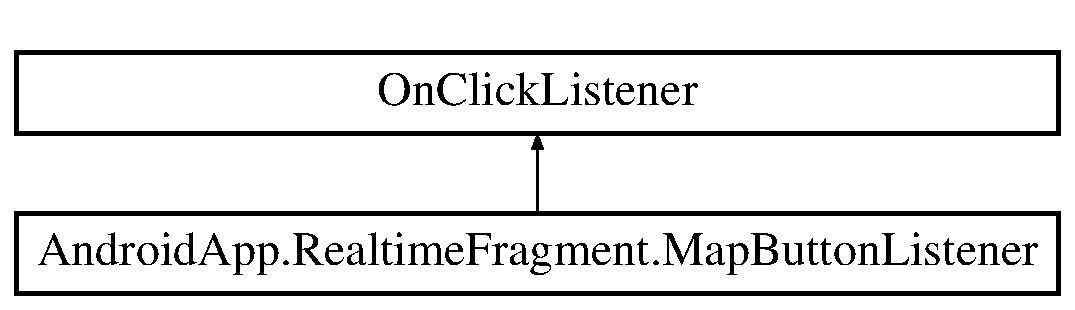
\includegraphics[height=2.000000cm]{class_android_app_1_1_realtime_fragment_1_1_map_button_listener}
\end{center}
\end{figure}
\subsection*{Public Member Functions}
\begin{DoxyCompactItemize}
\item 
void \hyperlink{class_android_app_1_1_realtime_fragment_1_1_map_button_listener_ad7242a00f24a6ed739742d0fdcb80676}{on\+Click} (View v)
\begin{DoxyCompactList}\small\item\em Function for handling when map button pressed. \end{DoxyCompactList}\end{DoxyCompactItemize}


\subsection{Detailed Description}
Listener for starting a map activity when button pressed. 

\subsection{Member Function Documentation}
\mbox{\Hypertarget{class_android_app_1_1_realtime_fragment_1_1_map_button_listener_ad7242a00f24a6ed739742d0fdcb80676}\label{class_android_app_1_1_realtime_fragment_1_1_map_button_listener_ad7242a00f24a6ed739742d0fdcb80676}} 
\index{Android\+App\+::\+Realtime\+Fragment\+::\+Map\+Button\+Listener@{Android\+App\+::\+Realtime\+Fragment\+::\+Map\+Button\+Listener}!on\+Click@{on\+Click}}
\index{on\+Click@{on\+Click}!Android\+App\+::\+Realtime\+Fragment\+::\+Map\+Button\+Listener@{Android\+App\+::\+Realtime\+Fragment\+::\+Map\+Button\+Listener}}
\subsubsection{\texorpdfstring{on\+Click()}{onClick()}}
{\footnotesize\ttfamily void Android\+App.\+Realtime\+Fragment.\+Map\+Button\+Listener.\+on\+Click (\begin{DoxyParamCaption}\item[{View}]{v }\end{DoxyParamCaption})\hspace{0.3cm}{\ttfamily [inline]}}



Function for handling when map button pressed. 

Created a new intent to start our map activity. Serialised statistics are then added as a bundle in the intent.


\begin{DoxyParams}{Parameters}
{\em v} & -\/ Current view of the button. \\
\hline
\end{DoxyParams}

\begin{DoxyCode}
193                                   \{
194           Intent intent = \textcolor{keyword}{new} Intent(getActivity(), MapsActivity.class);
195           intent.putExtra(\textcolor{stringliteral}{"JSONList"}, \hyperlink{class_android_app_1_1_realtime_fragment_a4c3f12bcaaab715dc512d4cd4a4c11cf}{jsonList});
196           startActivity(intent);
197       \}
\end{DoxyCode}


The documentation for this class was generated from the following file\+:\begin{DoxyCompactItemize}
\item 
android-\/app/app/src/main/java/com/jack/motorbikestatistics/\hyperlink{_realtime_fragment_8java}{Realtime\+Fragment.\+java}\end{DoxyCompactItemize}

\hypertarget{class_android_app_1_1_set_of_data_items}{}\section{Android\+App.\+Set\+Of\+Data\+Items Class Reference}
\label{class_android_app_1_1_set_of_data_items}\index{Android\+App.\+Set\+Of\+Data\+Items@{Android\+App.\+Set\+Of\+Data\+Items}}


Array\+List extension to allow searching via item name.  


Inheritance diagram for Android\+App.\+Set\+Of\+Data\+Items\+:\begin{figure}[H]
\begin{center}
\leavevmode
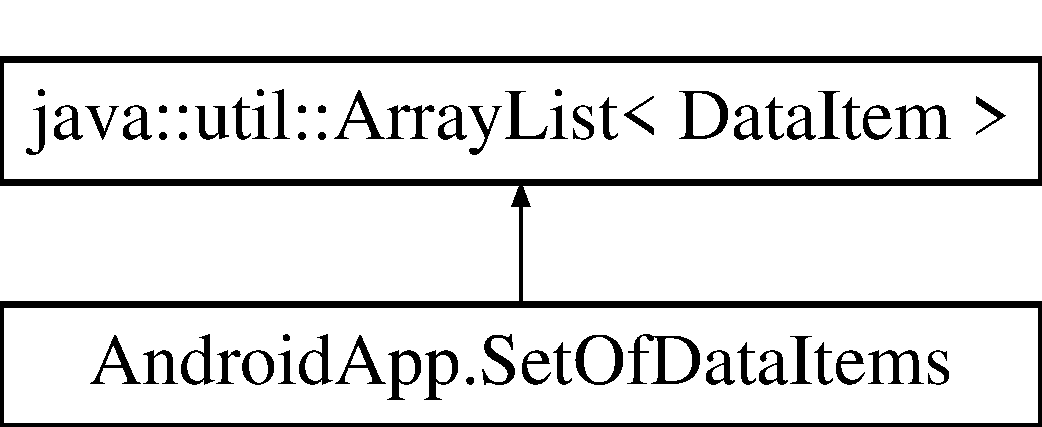
\includegraphics[height=2.000000cm]{class_android_app_1_1_set_of_data_items}
\end{center}
\end{figure}
\subsection*{Public Member Functions}
\begin{DoxyCompactItemize}
\item 
\mbox{\Hypertarget{class_android_app_1_1_set_of_data_items_a719c4dffae070925492a8cca986a8337}\label{class_android_app_1_1_set_of_data_items_a719c4dffae070925492a8cca986a8337}} 
\hyperlink{class_android_app_1_1_set_of_data_items_a719c4dffae070925492a8cca986a8337}{Set\+Of\+Data\+Items} ()
\begin{DoxyCompactList}\small\item\em Constructor, just calls inherited constructor method. \end{DoxyCompactList}\item 
\hyperlink{class_android_app_1_1_data_item}{Data\+Item} \hyperlink{class_android_app_1_1_set_of_data_items_aa559ef3701bb9f59f124ddddc56a2a38}{get\+Item\+By\+Name} (String name)
\begin{DoxyCompactList}\small\item\em Function to allow searching of Array\+List$<$\+Data\+Item$>$ via name. \end{DoxyCompactList}\end{DoxyCompactItemize}


\subsection{Detailed Description}
Array\+List extension to allow searching via item name. 

\subsection{Member Function Documentation}
\mbox{\Hypertarget{class_android_app_1_1_set_of_data_items_aa559ef3701bb9f59f124ddddc56a2a38}\label{class_android_app_1_1_set_of_data_items_aa559ef3701bb9f59f124ddddc56a2a38}} 
\index{Android\+App\+::\+Set\+Of\+Data\+Items@{Android\+App\+::\+Set\+Of\+Data\+Items}!get\+Item\+By\+Name@{get\+Item\+By\+Name}}
\index{get\+Item\+By\+Name@{get\+Item\+By\+Name}!Android\+App\+::\+Set\+Of\+Data\+Items@{Android\+App\+::\+Set\+Of\+Data\+Items}}
\subsubsection{\texorpdfstring{get\+Item\+By\+Name()}{getItemByName()}}
{\footnotesize\ttfamily \hyperlink{class_android_app_1_1_data_item}{Data\+Item} Android\+App.\+Set\+Of\+Data\+Items.\+get\+Item\+By\+Name (\begin{DoxyParamCaption}\item[{String}]{name }\end{DoxyParamCaption})\hspace{0.3cm}{\ttfamily [inline]}}



Function to allow searching of Array\+List$<$\+Data\+Item$>$ via name. 

Loops through all items in array until one item with matching name is found. This is then returned by the function.


\begin{DoxyParams}{Parameters}
{\em name} & -\/ Name to match. \\
\hline
\end{DoxyParams}
\begin{DoxyReturn}{Returns}
\hyperlink{class_android_app_1_1_data_item}{Data\+Item} -\/ The item with matching name. 
\end{DoxyReturn}


References Android\+App.\+Data\+Item$<$ T $>$.\+get\+Name().


\begin{DoxyCode}
36                                                \{
37         DataItem result = null;
38 
39         \textcolor{keywordflow}{for} (DataItem item: \textcolor{keyword}{this}) \{
40             \textcolor{keywordflow}{if} (item.getName().equals(name)) \{
41                 result = item;
42                 \textcolor{keywordflow}{break};
43             \}
44         \}
45 
46         \textcolor{keywordflow}{return} result;
47     \}
\end{DoxyCode}


The documentation for this class was generated from the following file\+:\begin{DoxyCompactItemize}
\item 
android-\/app/app/src/main/java/com/jack/motorbikestatistics/\hyperlink{_set_of_data_items_8java}{Set\+Of\+Data\+Items.\+java}\end{DoxyCompactItemize}

\hypertarget{class_android_app_1_1_trip_item}{}\section{Android\+App.\+Trip\+Item Class Reference}
\label{class_android_app_1_1_trip_item}\index{Android\+App.\+Trip\+Item@{Android\+App.\+Trip\+Item}}


Class used for holding name and size information relating to a trip.  


\subsection*{Public Member Functions}
\begin{DoxyCompactItemize}
\item 
\hyperlink{class_android_app_1_1_trip_item_a3ef9684be0d75a972fc373db43aa0efd}{Trip\+Item} (String name, int size)
\begin{DoxyCompactList}\small\item\em Constructor for creating of a \hyperlink{class_android_app_1_1_trip_item}{Trip\+Item}. \end{DoxyCompactList}\item 
String \hyperlink{class_android_app_1_1_trip_item_ae7d202ccb169b225ed3c7f5b6b0fb9eb}{get\+Trip\+Name} ()
\begin{DoxyCompactList}\small\item\em Getter for trip name. \end{DoxyCompactList}\item 
void \hyperlink{class_android_app_1_1_trip_item_a6c1705dd48325abf0a0abbda977df903}{set\+Trip\+Name} (String \hyperlink{class_android_app_1_1_trip_item_ae5137b0b6077e3fcf293430bc9c488e3}{trip\+Name})
\begin{DoxyCompactList}\small\item\em Setter for trip name. \end{DoxyCompactList}\item 
int \hyperlink{class_android_app_1_1_trip_item_a565ec50649fe1edf5db7301ec3f10497}{get\+File\+Size} ()
\begin{DoxyCompactList}\small\item\em Getter for trip filesize. \end{DoxyCompactList}\item 
void \hyperlink{class_android_app_1_1_trip_item_a85d328bdc6fd3d54c5c275aea2e23852}{set\+File\+Size} (int \hyperlink{class_android_app_1_1_trip_item_a0689a1340427784d8658cc616da310f2}{file\+Size})
\begin{DoxyCompactList}\small\item\em Setter for trip filesize. \end{DoxyCompactList}\end{DoxyCompactItemize}
\subsection*{Private Attributes}
\begin{DoxyCompactItemize}
\item 
\mbox{\Hypertarget{class_android_app_1_1_trip_item_ae5137b0b6077e3fcf293430bc9c488e3}\label{class_android_app_1_1_trip_item_ae5137b0b6077e3fcf293430bc9c488e3}} 
String \hyperlink{class_android_app_1_1_trip_item_ae5137b0b6077e3fcf293430bc9c488e3}{trip\+Name} = null
\begin{DoxyCompactList}\small\item\em The trips name on the u\+SD card. \end{DoxyCompactList}\item 
\mbox{\Hypertarget{class_android_app_1_1_trip_item_a0689a1340427784d8658cc616da310f2}\label{class_android_app_1_1_trip_item_a0689a1340427784d8658cc616da310f2}} 
int \hyperlink{class_android_app_1_1_trip_item_a0689a1340427784d8658cc616da310f2}{file\+Size} = 0
\begin{DoxyCompactList}\small\item\em The trips file size on the u\+SD card. \end{DoxyCompactList}\end{DoxyCompactItemize}


\subsection{Detailed Description}
Class used for holding name and size information relating to a trip. 

\subsection{Constructor \& Destructor Documentation}
\mbox{\Hypertarget{class_android_app_1_1_trip_item_a3ef9684be0d75a972fc373db43aa0efd}\label{class_android_app_1_1_trip_item_a3ef9684be0d75a972fc373db43aa0efd}} 
\index{Android\+App\+::\+Trip\+Item@{Android\+App\+::\+Trip\+Item}!Trip\+Item@{Trip\+Item}}
\index{Trip\+Item@{Trip\+Item}!Android\+App\+::\+Trip\+Item@{Android\+App\+::\+Trip\+Item}}
\subsubsection{\texorpdfstring{Trip\+Item()}{TripItem()}}
{\footnotesize\ttfamily Android\+App.\+Trip\+Item.\+Trip\+Item (\begin{DoxyParamCaption}\item[{String}]{name,  }\item[{int}]{size }\end{DoxyParamCaption})\hspace{0.3cm}{\ttfamily [inline]}}



Constructor for creating of a \hyperlink{class_android_app_1_1_trip_item}{Trip\+Item}. 

Sets the original file name and size.


\begin{DoxyParams}{Parameters}
{\em name} & -\/ Trip name. \\
\hline
{\em size} & -\/ Size of the file. \\
\hline
\end{DoxyParams}

\begin{DoxyCode}
31                                            \{
32         this.\hyperlink{class_android_app_1_1_trip_item_ae5137b0b6077e3fcf293430bc9c488e3}{tripName} = name;
33         this.\hyperlink{class_android_app_1_1_trip_item_a0689a1340427784d8658cc616da310f2}{fileSize} = size;
34     \}
\end{DoxyCode}


\subsection{Member Function Documentation}
\mbox{\Hypertarget{class_android_app_1_1_trip_item_ae7d202ccb169b225ed3c7f5b6b0fb9eb}\label{class_android_app_1_1_trip_item_ae7d202ccb169b225ed3c7f5b6b0fb9eb}} 
\index{Android\+App\+::\+Trip\+Item@{Android\+App\+::\+Trip\+Item}!get\+Trip\+Name@{get\+Trip\+Name}}
\index{get\+Trip\+Name@{get\+Trip\+Name}!Android\+App\+::\+Trip\+Item@{Android\+App\+::\+Trip\+Item}}
\subsubsection{\texorpdfstring{get\+Trip\+Name()}{getTripName()}}
{\footnotesize\ttfamily String Android\+App.\+Trip\+Item.\+get\+Trip\+Name (\begin{DoxyParamCaption}{ }\end{DoxyParamCaption})\hspace{0.3cm}{\ttfamily [inline]}}



Getter for trip name. 

\begin{DoxyReturn}{Returns}
String -\/ Trip name. 
\end{DoxyReturn}

\begin{DoxyCode}
40                                 \{
41         \textcolor{keywordflow}{return} \hyperlink{class_android_app_1_1_trip_item_ae5137b0b6077e3fcf293430bc9c488e3}{tripName};
42     \}
\end{DoxyCode}
\mbox{\Hypertarget{class_android_app_1_1_trip_item_a6c1705dd48325abf0a0abbda977df903}\label{class_android_app_1_1_trip_item_a6c1705dd48325abf0a0abbda977df903}} 
\index{Android\+App\+::\+Trip\+Item@{Android\+App\+::\+Trip\+Item}!set\+Trip\+Name@{set\+Trip\+Name}}
\index{set\+Trip\+Name@{set\+Trip\+Name}!Android\+App\+::\+Trip\+Item@{Android\+App\+::\+Trip\+Item}}
\subsubsection{\texorpdfstring{set\+Trip\+Name()}{setTripName()}}
{\footnotesize\ttfamily void Android\+App.\+Trip\+Item.\+set\+Trip\+Name (\begin{DoxyParamCaption}\item[{String}]{trip\+Name }\end{DoxyParamCaption})\hspace{0.3cm}{\ttfamily [inline]}}



Setter for trip name. 


\begin{DoxyParams}{Parameters}
{\em trip\+Name} & -\/ New trip name. \\
\hline
\end{DoxyParams}

\begin{DoxyCode}
48                                              \{
49         this.\hyperlink{class_android_app_1_1_trip_item_ae5137b0b6077e3fcf293430bc9c488e3}{tripName} = \hyperlink{class_android_app_1_1_trip_item_ae5137b0b6077e3fcf293430bc9c488e3}{tripName};
50     \}
\end{DoxyCode}
\mbox{\Hypertarget{class_android_app_1_1_trip_item_a565ec50649fe1edf5db7301ec3f10497}\label{class_android_app_1_1_trip_item_a565ec50649fe1edf5db7301ec3f10497}} 
\index{Android\+App\+::\+Trip\+Item@{Android\+App\+::\+Trip\+Item}!get\+File\+Size@{get\+File\+Size}}
\index{get\+File\+Size@{get\+File\+Size}!Android\+App\+::\+Trip\+Item@{Android\+App\+::\+Trip\+Item}}
\subsubsection{\texorpdfstring{get\+File\+Size()}{getFileSize()}}
{\footnotesize\ttfamily int Android\+App.\+Trip\+Item.\+get\+File\+Size (\begin{DoxyParamCaption}{ }\end{DoxyParamCaption})\hspace{0.3cm}{\ttfamily [inline]}}



Getter for trip filesize. 

\begin{DoxyReturn}{Returns}
int -\/ Filesize in bytes. 
\end{DoxyReturn}

\begin{DoxyCode}
56                              \{
57         \textcolor{keywordflow}{return} \hyperlink{class_android_app_1_1_trip_item_a0689a1340427784d8658cc616da310f2}{fileSize};
58     \}
\end{DoxyCode}
\mbox{\Hypertarget{class_android_app_1_1_trip_item_a85d328bdc6fd3d54c5c275aea2e23852}\label{class_android_app_1_1_trip_item_a85d328bdc6fd3d54c5c275aea2e23852}} 
\index{Android\+App\+::\+Trip\+Item@{Android\+App\+::\+Trip\+Item}!set\+File\+Size@{set\+File\+Size}}
\index{set\+File\+Size@{set\+File\+Size}!Android\+App\+::\+Trip\+Item@{Android\+App\+::\+Trip\+Item}}
\subsubsection{\texorpdfstring{set\+File\+Size()}{setFileSize()}}
{\footnotesize\ttfamily void Android\+App.\+Trip\+Item.\+set\+File\+Size (\begin{DoxyParamCaption}\item[{int}]{file\+Size }\end{DoxyParamCaption})\hspace{0.3cm}{\ttfamily [inline]}}



Setter for trip filesize. 


\begin{DoxyParams}{Parameters}
{\em file\+Size} & -\/ New trip filesize. \\
\hline
\end{DoxyParams}

\begin{DoxyCode}
64                                           \{
65         \textcolor{keywordflow}{if} (\hyperlink{class_android_app_1_1_trip_item_a0689a1340427784d8658cc616da310f2}{fileSize} >= 0) \{
66             this.\hyperlink{class_android_app_1_1_trip_item_a0689a1340427784d8658cc616da310f2}{fileSize} = \hyperlink{class_android_app_1_1_trip_item_a0689a1340427784d8658cc616da310f2}{fileSize};
67         \}
68     \}
\end{DoxyCode}


The documentation for this class was generated from the following file\+:\begin{DoxyCompactItemize}
\item 
android-\/app/app/src/main/java/com/jack/motorbikestatistics/\hyperlink{_trip_item_8java}{Trip\+Item.\+java}\end{DoxyCompactItemize}

\hypertarget{class_android_app_1_1_trip_list_adapter}{}\section{Android\+App.\+Trip\+List\+Adapter Class Reference}
\label{class_android_app_1_1_trip_list_adapter}\index{Android\+App.\+Trip\+List\+Adapter@{Android\+App.\+Trip\+List\+Adapter}}


Adapter class used for displaying all trips.  


Inheritance diagram for Android\+App.\+Trip\+List\+Adapter\+:\begin{figure}[H]
\begin{center}
\leavevmode
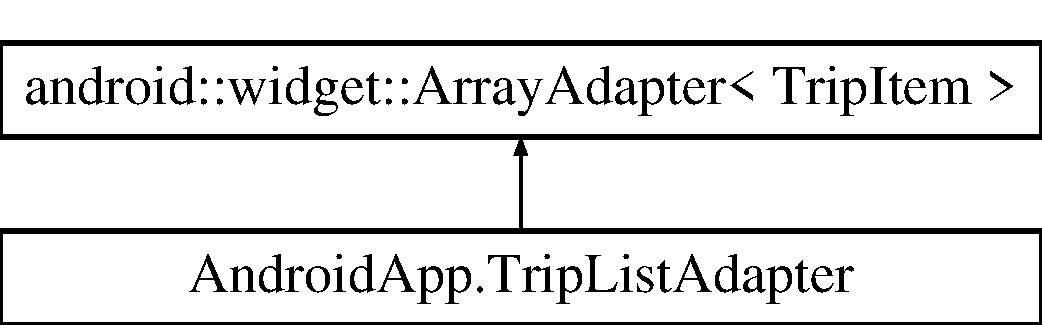
\includegraphics[height=2.000000cm]{class_android_app_1_1_trip_list_adapter}
\end{center}
\end{figure}
\subsection*{Classes}
\begin{DoxyCompactItemize}
\item 
class \hyperlink{class_android_app_1_1_trip_list_adapter_1_1_view_holder}{View\+Holder}
\begin{DoxyCompactList}\small\item\em Class that holds all UI data to be displayed for each List\+Item. \end{DoxyCompactList}\end{DoxyCompactItemize}
\subsection*{Public Member Functions}
\begin{DoxyCompactItemize}
\item 
\hyperlink{class_android_app_1_1_trip_list_adapter_ad8d8c6f5a394a8d7e6e97d5bf239af76}{Trip\+List\+Adapter} (Context cnt, int \hyperlink{class_android_app_1_1_trip_list_adapter_a57cb58f32f3b9ea25c6330a821cb8455}{layout\+Resource\+Id}, Array\+List$<$ \hyperlink{class_android_app_1_1_trip_item}{Trip\+Item} $>$ \hyperlink{class_android_app_1_1_trip_list_adapter_a8cea45e06b19821352bce2de9b3e3941}{data})
\begin{DoxyCompactList}\small\item\em Constructor for the List\+View adapter. \end{DoxyCompactList}\item 
View \hyperlink{class_android_app_1_1_trip_list_adapter_aecaed2759c3d4753c8472cef9e731b01}{get\+View} (int position, View convert\+View, View\+Group parent)
\begin{DoxyCompactList}\small\item\em Function for returning the view of each list item (\hyperlink{class_android_app_1_1_trip_item}{Trip\+Item}). \end{DoxyCompactList}\end{DoxyCompactItemize}
\subsection*{Private Attributes}
\begin{DoxyCompactItemize}
\item 
\mbox{\Hypertarget{class_android_app_1_1_trip_list_adapter_a14fa25bc6de0af86497d0cce3e0bdc1b}\label{class_android_app_1_1_trip_list_adapter_a14fa25bc6de0af86497d0cce3e0bdc1b}} 
Context \hyperlink{class_android_app_1_1_trip_list_adapter_a14fa25bc6de0af86497d0cce3e0bdc1b}{context}
\begin{DoxyCompactList}\small\item\em Context that the List\+View is operating in. \end{DoxyCompactList}\item 
\mbox{\Hypertarget{class_android_app_1_1_trip_list_adapter_a57cb58f32f3b9ea25c6330a821cb8455}\label{class_android_app_1_1_trip_list_adapter_a57cb58f32f3b9ea25c6330a821cb8455}} 
int \hyperlink{class_android_app_1_1_trip_list_adapter_a57cb58f32f3b9ea25c6330a821cb8455}{layout\+Resource\+Id}
\begin{DoxyCompactList}\small\item\em Resource ID for current layout. \end{DoxyCompactList}\item 
\mbox{\Hypertarget{class_android_app_1_1_trip_list_adapter_a8cea45e06b19821352bce2de9b3e3941}\label{class_android_app_1_1_trip_list_adapter_a8cea45e06b19821352bce2de9b3e3941}} 
Array\+List$<$ \hyperlink{class_android_app_1_1_trip_item}{Trip\+Item} $>$ \hyperlink{class_android_app_1_1_trip_list_adapter_a8cea45e06b19821352bce2de9b3e3941}{data}
\begin{DoxyCompactList}\small\item\em Array\+List of all trip items to display. \end{DoxyCompactList}\end{DoxyCompactItemize}


\subsection{Detailed Description}
Adapter class used for displaying all trips. 

\subsection{Constructor \& Destructor Documentation}
\mbox{\Hypertarget{class_android_app_1_1_trip_list_adapter_ad8d8c6f5a394a8d7e6e97d5bf239af76}\label{class_android_app_1_1_trip_list_adapter_ad8d8c6f5a394a8d7e6e97d5bf239af76}} 
\index{Android\+App\+::\+Trip\+List\+Adapter@{Android\+App\+::\+Trip\+List\+Adapter}!Trip\+List\+Adapter@{Trip\+List\+Adapter}}
\index{Trip\+List\+Adapter@{Trip\+List\+Adapter}!Android\+App\+::\+Trip\+List\+Adapter@{Android\+App\+::\+Trip\+List\+Adapter}}
\subsubsection{\texorpdfstring{Trip\+List\+Adapter()}{TripListAdapter()}}
{\footnotesize\ttfamily Android\+App.\+Trip\+List\+Adapter.\+Trip\+List\+Adapter (\begin{DoxyParamCaption}\item[{Context}]{cnt,  }\item[{int}]{layout\+Resource\+Id,  }\item[{Array\+List$<$ \hyperlink{class_android_app_1_1_trip_item}{Trip\+Item} $>$}]{data }\end{DoxyParamCaption})\hspace{0.3cm}{\ttfamily [inline]}}



Constructor for the List\+View adapter. 

Calls the constructor of the superclass as well as setting other relevant information needed.


\begin{DoxyParams}{Parameters}
{\em cnt} & -\/ Context of the adapter to be operating in. \\
\hline
{\em layout\+Resource\+Id} & -\/ Resource ID for current layout. \\
\hline
{\em data} & -\/ Array\+List of statistics to display in List\+View. \\
\hline
\end{DoxyParams}

\begin{DoxyCode}
47                                                                                         \{
48         super(cnt, \hyperlink{class_android_app_1_1_trip_list_adapter_a57cb58f32f3b9ea25c6330a821cb8455}{layoutResourceId}, \hyperlink{class_android_app_1_1_trip_list_adapter_a8cea45e06b19821352bce2de9b3e3941}{data});
49 
50         this.\hyperlink{class_android_app_1_1_trip_list_adapter_a14fa25bc6de0af86497d0cce3e0bdc1b}{context} = cnt;
51         this.\hyperlink{class_android_app_1_1_trip_list_adapter_a57cb58f32f3b9ea25c6330a821cb8455}{layoutResourceId} = \hyperlink{class_android_app_1_1_trip_list_adapter_a57cb58f32f3b9ea25c6330a821cb8455}{layoutResourceId};
52         this.\hyperlink{class_android_app_1_1_trip_list_adapter_a8cea45e06b19821352bce2de9b3e3941}{data} = \hyperlink{class_android_app_1_1_trip_list_adapter_a8cea45e06b19821352bce2de9b3e3941}{data};
53     \}
\end{DoxyCode}


\subsection{Member Function Documentation}
\mbox{\Hypertarget{class_android_app_1_1_trip_list_adapter_aecaed2759c3d4753c8472cef9e731b01}\label{class_android_app_1_1_trip_list_adapter_aecaed2759c3d4753c8472cef9e731b01}} 
\index{Android\+App\+::\+Trip\+List\+Adapter@{Android\+App\+::\+Trip\+List\+Adapter}!get\+View@{get\+View}}
\index{get\+View@{get\+View}!Android\+App\+::\+Trip\+List\+Adapter@{Android\+App\+::\+Trip\+List\+Adapter}}
\subsubsection{\texorpdfstring{get\+View()}{getView()}}
{\footnotesize\ttfamily View Android\+App.\+Trip\+List\+Adapter.\+get\+View (\begin{DoxyParamCaption}\item[{int}]{position,  }\item[{View}]{convert\+View,  }\item[{View\+Group}]{parent }\end{DoxyParamCaption})\hspace{0.3cm}{\ttfamily [inline]}}



Function for returning the view of each list item (\hyperlink{class_android_app_1_1_trip_item}{Trip\+Item}). 

If a view for selected item has not been created inflater initialises it. A holder is then used to hold all the information that will be displayed on the UI to the user.


\begin{DoxyParams}{Parameters}
{\em position} & -\/ Index of item in array to use/reference to. \\
\hline
{\em convert\+View} & -\/ View to be used for specified item. \\
\hline
{\em parent} & -\/ Object where the created view will be placed on. \\
\hline
\end{DoxyParams}
\begin{DoxyReturn}{Returns}
View -\/ The result view of item with updated/current information. 
\end{DoxyReturn}


References Android\+App.\+Trip\+Item.\+get\+File\+Size(), and Android\+App.\+Trip\+Item.\+get\+Trip\+Name().


\begin{DoxyCode}
77                                                                           \{
78         ViewHolder holder;
79 
80         \textcolor{keywordflow}{if} (convertView == null)
81         \{
82             \textcolor{comment}{/* If view does not already exist. */}
83             LayoutInflater inflater = (LayoutInflater)\hyperlink{class_android_app_1_1_trip_list_adapter_a14fa25bc6de0af86497d0cce3e0bdc1b}{context}.getSystemService(Context.
      LAYOUT\_INFLATER\_SERVICE);
84             convertView = inflater.inflate(\hyperlink{class_android_app_1_1_trip_list_adapter_a57cb58f32f3b9ea25c6330a821cb8455}{layoutResourceId}, parent, \textcolor{keyword}{false});
85 
86             holder = \textcolor{keyword}{new} ViewHolder();
87             holder.name = (TextView)convertView.findViewById(R.id.triplist\_name);
88             holder.fileSize = (TextView)convertView.findViewById(R.id.triplist\_size);
89             convertView.setTag(holder);
90         \}
91         \textcolor{keywordflow}{else}
92         \{
93             \textcolor{comment}{/* If view already exists. */}
94             holder = (ViewHolder)convertView.getTag();
95         \}
96 
97         TripItem tripItem = getItem(position);
98 
99         \textcolor{comment}{/* Set our holder with current data of item */}
100         holder.name.setText(tripItem.getTripName());
101         holder.fileSize.setText(Integer.toString(tripItem.getFileSize()));
102 
103         \textcolor{keywordflow}{return} convertView;
104     \}
\end{DoxyCode}


The documentation for this class was generated from the following file\+:\begin{DoxyCompactItemize}
\item 
android-\/app/app/src/main/java/com/jack/motorbikestatistics/\hyperlink{_trip_list_adapter_8java}{Trip\+List\+Adapter.\+java}\end{DoxyCompactItemize}

\hypertarget{class_android_app_1_1_trip_list_adapter_1_1_view_holder}{}\section{Android\+App.\+Trip\+List\+Adapter.\+View\+Holder Class Reference}
\label{class_android_app_1_1_trip_list_adapter_1_1_view_holder}\index{Android\+App.\+Trip\+List\+Adapter.\+View\+Holder@{Android\+App.\+Trip\+List\+Adapter.\+View\+Holder}}


Class that holds all UI data to be displayed for each List\+Item.  




\subsection{Detailed Description}
Class that holds all UI data to be displayed for each List\+Item. 

The documentation for this class was generated from the following file\+:\begin{DoxyCompactItemize}
\item 
android-\/app/app/src/main/java/com/jack/motorbikestatistics/\hyperlink{_trip_list_adapter_8java}{Trip\+List\+Adapter.\+java}\end{DoxyCompactItemize}

\hypertarget{class_logging_device_1_1_orientation}{}\section{Logging\+Device\+:\+:Orientation Class Reference}
\label{class_logging_device_1_1_orientation}\index{Logging\+Device\+::\+Orientation@{Logging\+Device\+::\+Orientation}}


Class for dealing with \hyperlink{class_logging_device_1_1_orientation}{Orientation} functionality on logging device.  




{\ttfamily \#include $<$Orientation.\+h$>$}

\subsection*{Public Member Functions}
\begin{DoxyCompactItemize}
\item 
void \hyperlink{class_logging_device_1_1_orientation_a317461c5c8afa8c3abf56847d4544728}{init} ()
\begin{DoxyCompactList}\small\item\em Initialisation function for orientation module. \end{DoxyCompactList}\item 
bool \hyperlink{class_logging_device_1_1_orientation_aad568a473f999c181abac46a4d832387}{poll\+I\+MU} ()
\begin{DoxyCompactList}\small\item\em Updates the I\+MU with newest values at 25\+Hz frequency. \end{DoxyCompactList}\item 
float \hyperlink{class_logging_device_1_1_orientation_a3dbaa1ee014811c40d5b9f39b544c19b}{get\+Yaw} ()
\begin{DoxyCompactList}\small\item\em Returns the Yaw orientation of the device. \end{DoxyCompactList}\item 
float \hyperlink{class_logging_device_1_1_orientation_a7ec1a2964fc858bbd5da22a505b087c8}{get\+Pitch} ()
\begin{DoxyCompactList}\small\item\em Returns the Pitch orientation of the device. \end{DoxyCompactList}\item 
float \hyperlink{class_logging_device_1_1_orientation_ab8923432cb8c18822b0a9ae95a5ac505}{get\+Roll} ()
\begin{DoxyCompactList}\small\item\em Returns the Roll orientation of the device. \end{DoxyCompactList}\end{DoxyCompactItemize}
\subsection*{Private Member Functions}
\begin{DoxyCompactItemize}
\item 
float \hyperlink{class_logging_device_1_1_orientation_ab8a6f65b7f2b43ec5dd09c47fe93fa0b}{convert\+Raw\+Accel} (int a\+Raw)
\begin{DoxyCompactList}\small\item\em Converts a raw reading from accelerometer to a value in G. \end{DoxyCompactList}\item 
float \hyperlink{class_logging_device_1_1_orientation_a99bb5ed3c3226c5d636fa48f26f491dd}{convert\+Raw\+Gyro} (int a\+Raw)
\begin{DoxyCompactList}\small\item\em Converts a raw reading from gyro to a value in deg/sec. \end{DoxyCompactList}\end{DoxyCompactItemize}
\subsection*{Private Attributes}
\begin{DoxyCompactItemize}
\item 
\mbox{\Hypertarget{class_logging_device_1_1_orientation_a517282a58a498881d97d57f4829a38d9}\label{class_logging_device_1_1_orientation_a517282a58a498881d97d57f4829a38d9}} 
Madgwick \hyperlink{class_logging_device_1_1_orientation_a517282a58a498881d97d57f4829a38d9}{I\+M\+Ufilter}
\begin{DoxyCompactList}\small\item\em Madgwick filter object uses to steady orientation readings. \end{DoxyCompactList}\end{DoxyCompactItemize}


\subsection{Detailed Description}
Class for dealing with \hyperlink{class_logging_device_1_1_orientation}{Orientation} functionality on logging device. 

\subsection{Member Function Documentation}
\mbox{\Hypertarget{class_logging_device_1_1_orientation_ab8a6f65b7f2b43ec5dd09c47fe93fa0b}\label{class_logging_device_1_1_orientation_ab8a6f65b7f2b43ec5dd09c47fe93fa0b}} 
\index{Logging\+Device\+::\+Orientation@{Logging\+Device\+::\+Orientation}!convert\+Raw\+Accel@{convert\+Raw\+Accel}}
\index{convert\+Raw\+Accel@{convert\+Raw\+Accel}!Logging\+Device\+::\+Orientation@{Logging\+Device\+::\+Orientation}}
\subsubsection{\texorpdfstring{convert\+Raw\+Accel()}{convertRawAccel()}}
{\footnotesize\ttfamily float Orientation\+::convert\+Raw\+Accel (\begin{DoxyParamCaption}\item[{int}]{a\+Raw }\end{DoxyParamCaption})\hspace{0.3cm}{\ttfamily [private]}}



Converts a raw reading from accelerometer to a value in G. 


\begin{DoxyParams}{Parameters}
{\em a\+Raw} & -\/ Raw accelerometer axis value. \\
\hline
\end{DoxyParams}
\begin{DoxyReturn}{Returns}
float -\/ Processed acceleration axis in G. 
\end{DoxyReturn}


References A\+C\+C\+E\+L\+\_\+\+R\+A\+N\+GE.


\begin{DoxyCode}
118 \{
119   \textcolor{comment}{/*}
120 \textcolor{comment}{   * Since using 2G range.}
121 \textcolor{comment}{   * -2G maps to raw value of -32768}
122 \textcolor{comment}{   * +2G maps to raw value of +32767}
123 \textcolor{comment}{   */}
124    \textcolor{keywordtype}{float} a = (aRaw * (float)\hyperlink{_orientation_8cpp_a16ec7011dea5773b504e875852f35fc1}{ACCEL\_RANGE}) / 32768.0;
125    \textcolor{keywordflow}{return} a;
126 \}
\end{DoxyCode}
\mbox{\Hypertarget{class_logging_device_1_1_orientation_a99bb5ed3c3226c5d636fa48f26f491dd}\label{class_logging_device_1_1_orientation_a99bb5ed3c3226c5d636fa48f26f491dd}} 
\index{Logging\+Device\+::\+Orientation@{Logging\+Device\+::\+Orientation}!convert\+Raw\+Gyro@{convert\+Raw\+Gyro}}
\index{convert\+Raw\+Gyro@{convert\+Raw\+Gyro}!Logging\+Device\+::\+Orientation@{Logging\+Device\+::\+Orientation}}
\subsubsection{\texorpdfstring{convert\+Raw\+Gyro()}{convertRawGyro()}}
{\footnotesize\ttfamily float Orientation\+::convert\+Raw\+Gyro (\begin{DoxyParamCaption}\item[{int}]{g\+Raw }\end{DoxyParamCaption})\hspace{0.3cm}{\ttfamily [private]}}



Converts a raw reading from gyro to a value in deg/sec. 


\begin{DoxyParams}{Parameters}
{\em g\+Raw} & -\/ Raw gyroscope axis value. \\
\hline
\end{DoxyParams}
\begin{DoxyReturn}{Returns}
float -\/ Processed rotation axis in deg/sec. 
\end{DoxyReturn}


References G\+Y\+R\+O\+\_\+\+R\+A\+N\+GE.


\begin{DoxyCode}
135 \{
136   \textcolor{comment}{/*}
137 \textcolor{comment}{   * since we are using 250 degrees/seconds range}
138 \textcolor{comment}{   * -250 maps to a raw value of -32768}
139 \textcolor{comment}{   * +250 maps to a raw value of 32767}
140 \textcolor{comment}{   */}
141   \textcolor{keywordtype}{float} g = (gRaw * (float)\hyperlink{_orientation_8cpp_af9a0775d43604d7410e3da3dbc90925a}{GYRO\_RANGE}) / 32768.0;
142   \textcolor{keywordflow}{return} g;
143 \}
\end{DoxyCode}
\mbox{\Hypertarget{class_logging_device_1_1_orientation_a317461c5c8afa8c3abf56847d4544728}\label{class_logging_device_1_1_orientation_a317461c5c8afa8c3abf56847d4544728}} 
\index{Logging\+Device\+::\+Orientation@{Logging\+Device\+::\+Orientation}!init@{init}}
\index{init@{init}!Logging\+Device\+::\+Orientation@{Logging\+Device\+::\+Orientation}}
\subsubsection{\texorpdfstring{init()}{init()}}
{\footnotesize\ttfamily void Orientation\+::init (\begin{DoxyParamCaption}{ }\end{DoxyParamCaption})}



Initialisation function for orientation module. 

Initialises the Curie\+I\+MU module with set ranges and rates, our Madgwick filter is also initialised with this information. 

References A\+C\+C\+E\+L\+\_\+\+R\+A\+N\+GE, G\+Y\+R\+O\+\_\+\+R\+A\+N\+GE, I\+M\+U\+\_\+\+F\+R\+E\+Q\+U\+E\+N\+CY, and I\+M\+Ufilter.


\begin{DoxyCode}
46 \{
47   \textcolor{comment}{/* Set up the Gyroscope + Accelerometer */}
48   CurieIMU.begin();
49   CurieIMU.setGyroRate(\hyperlink{_orientation_8cpp_aacb21c2e16f8c38c985b8f02787a7baf}{IMU\_FREQUENCY});
50   CurieIMU.setAccelerometerRate(\hyperlink{_orientation_8cpp_aacb21c2e16f8c38c985b8f02787a7baf}{IMU\_FREQUENCY});
51   CurieIMU.setAccelerometerRange(\hyperlink{_orientation_8cpp_a16ec7011dea5773b504e875852f35fc1}{ACCEL\_RANGE});
52   CurieIMU.setGyroRange(\hyperlink{_orientation_8cpp_af9a0775d43604d7410e3da3dbc90925a}{GYRO\_RANGE});
53 
54   \hyperlink{class_logging_device_1_1_orientation_a517282a58a498881d97d57f4829a38d9}{IMUfilter}.begin(\hyperlink{_orientation_8cpp_aacb21c2e16f8c38c985b8f02787a7baf}{IMU\_FREQUENCY});
55 \}
\end{DoxyCode}
\mbox{\Hypertarget{class_logging_device_1_1_orientation_aad568a473f999c181abac46a4d832387}\label{class_logging_device_1_1_orientation_aad568a473f999c181abac46a4d832387}} 
\index{Logging\+Device\+::\+Orientation@{Logging\+Device\+::\+Orientation}!poll\+I\+MU@{poll\+I\+MU}}
\index{poll\+I\+MU@{poll\+I\+MU}!Logging\+Device\+::\+Orientation@{Logging\+Device\+::\+Orientation}}
\subsubsection{\texorpdfstring{poll\+I\+M\+U()}{pollIMU()}}
{\footnotesize\ttfamily bool Orientation\+::poll\+I\+MU (\begin{DoxyParamCaption}{ }\end{DoxyParamCaption})}



Updates the I\+MU with newest values at 25\+Hz frequency. 

Function reads raw values from accelerometer and gyroscope and sends them to our Madgwick filter (I\+M\+Ufilter). ~\newline
This function needs to be called by the system as often as possible. ~\newline
To ensure correct frequency of 25\+Hz if kept to a micros counter is in place. ~\newline
Function will return true or false as of whether that call actually updated the I\+MU (depending on micros count check).

\begin{DoxyReturn}{Returns}
bool -\/ Whether the I\+MU was actually updated. 
\end{DoxyReturn}


References A\+X\+I\+S\+\_\+X, A\+X\+I\+S\+\_\+Y, A\+X\+I\+S\+\_\+Z, convert\+Raw\+Accel(), convert\+Raw\+Gyro(), I\+M\+U\+\_\+\+F\+R\+E\+Q\+U\+E\+N\+CY, I\+M\+Ufilter, and N\+U\+M\+B\+E\+R\+\_\+\+A\+X\+IS.


\begin{DoxyCode}
71 \{
72   \textcolor{keyword}{static} \textcolor{keyword}{const} \textcolor{keywordtype}{unsigned} \textcolor{keywordtype}{long} US\_PER\_READING = 1000000 / \hyperlink{_orientation_8cpp_aacb21c2e16f8c38c985b8f02787a7baf}{IMU\_FREQUENCY};
73   \textcolor{keyword}{static} \textcolor{keywordtype}{unsigned} \textcolor{keywordtype}{long} usPrevious = micros();
74 
75   \textcolor{keywordtype}{bool} result = \textcolor{keyword}{false};
76   \textcolor{keywordtype}{int} accel\_raw[\hyperlink{_orientation_8cpp_a203c415ee0716aeaf05afca2a736a9dc}{NUMBER\_AXIS}];
77   \textcolor{keywordtype}{int} gyro\_raw[\hyperlink{_orientation_8cpp_a203c415ee0716aeaf05afca2a736a9dc}{NUMBER\_AXIS}];
78   \textcolor{keywordtype}{float} accel\_g[\hyperlink{_orientation_8cpp_a203c415ee0716aeaf05afca2a736a9dc}{NUMBER\_AXIS}];
79   \textcolor{keywordtype}{float} gyro\_ds[\hyperlink{_orientation_8cpp_a203c415ee0716aeaf05afca2a736a9dc}{NUMBER\_AXIS}];
80   \textcolor{keywordtype}{unsigned} \textcolor{keywordtype}{long} usNow;
81 
82   \textcolor{comment}{/* Ensures we stick to the sample rate (by not sampling too early) */}
83   usNow = micros();
84   \textcolor{keywordflow}{if} ((usNow - usPrevious) >= US\_PER\_READING)
85   \{
86     \textcolor{comment}{/* Read raw data from the IMU */}
87     CurieIMU.readMotionSensor(accel\_raw[\hyperlink{_orientation_8cpp_a753faa457a1c2937ea3fdcdb83c3ca5f}{AXIS\_X}], accel\_raw[\hyperlink{_orientation_8cpp_a08f3e26d90cf66bf2840d476e5d4711f}{AXIS\_Y}], accel\_raw[
      \hyperlink{_orientation_8cpp_a220ebc22eb87c8989bfd63ae3cbbe2a8}{AXIS\_Z}],
88                               gyro\_raw[AXIS\_X], gyro\_raw[AXIS\_Y], gyro\_raw[AXIS\_Z]);
89 
90     \textcolor{comment}{/* Convert raw readings from IMU to accel (G) and rotation vel (deg/s) */}
91     accel\_g[\hyperlink{_orientation_8cpp_a753faa457a1c2937ea3fdcdb83c3ca5f}{AXIS\_X}] = \hyperlink{class_logging_device_1_1_orientation_ab8a6f65b7f2b43ec5dd09c47fe93fa0b}{convertRawAccel}(accel\_raw[AXIS\_X]);
92     accel\_g[\hyperlink{_orientation_8cpp_a08f3e26d90cf66bf2840d476e5d4711f}{AXIS\_Y}] = \hyperlink{class_logging_device_1_1_orientation_ab8a6f65b7f2b43ec5dd09c47fe93fa0b}{convertRawAccel}(accel\_raw[AXIS\_Y]);
93     accel\_g[\hyperlink{_orientation_8cpp_a220ebc22eb87c8989bfd63ae3cbbe2a8}{AXIS\_Z}] = \hyperlink{class_logging_device_1_1_orientation_ab8a6f65b7f2b43ec5dd09c47fe93fa0b}{convertRawAccel}(accel\_raw[AXIS\_Z]);
94     gyro\_ds[\hyperlink{_orientation_8cpp_a753faa457a1c2937ea3fdcdb83c3ca5f}{AXIS\_X}] = \hyperlink{class_logging_device_1_1_orientation_a99bb5ed3c3226c5d636fa48f26f491dd}{convertRawGyro}(gyro\_raw[AXIS\_X]);
95     gyro\_ds[\hyperlink{_orientation_8cpp_a08f3e26d90cf66bf2840d476e5d4711f}{AXIS\_Y}] = \hyperlink{class_logging_device_1_1_orientation_a99bb5ed3c3226c5d636fa48f26f491dd}{convertRawGyro}(gyro\_raw[AXIS\_Y]);
96     gyro\_ds[\hyperlink{_orientation_8cpp_a220ebc22eb87c8989bfd63ae3cbbe2a8}{AXIS\_Z}] = \hyperlink{class_logging_device_1_1_orientation_a99bb5ed3c3226c5d636fa48f26f491dd}{convertRawGyro}(gyro\_raw[AXIS\_Z]);
97 
98     \textcolor{comment}{/* Update the filter. Orientation is calculated here */}
99     \hyperlink{class_logging_device_1_1_orientation_a517282a58a498881d97d57f4829a38d9}{IMUfilter}.updateIMU(gyro\_ds[AXIS\_X], gyro\_ds[AXIS\_Y], gyro\_ds[AXIS\_Z],
100                         accel\_g[AXIS\_X], accel\_g[AXIS\_Y], accel\_g[AXIS\_Z]);
101 
102     \textcolor{comment}{/* Increment previous counter */}
103     usPrevious += US\_PER\_READING;
104 
105     result = \textcolor{keyword}{true};
106   \}
107 
108   \textcolor{keywordflow}{return} result;
109 \}
\end{DoxyCode}
\mbox{\Hypertarget{class_logging_device_1_1_orientation_a3dbaa1ee014811c40d5b9f39b544c19b}\label{class_logging_device_1_1_orientation_a3dbaa1ee014811c40d5b9f39b544c19b}} 
\index{Logging\+Device\+::\+Orientation@{Logging\+Device\+::\+Orientation}!get\+Yaw@{get\+Yaw}}
\index{get\+Yaw@{get\+Yaw}!Logging\+Device\+::\+Orientation@{Logging\+Device\+::\+Orientation}}
\subsubsection{\texorpdfstring{get\+Yaw()}{getYaw()}}
{\footnotesize\ttfamily float Orientation\+::get\+Yaw (\begin{DoxyParamCaption}{ }\end{DoxyParamCaption})}



Returns the Yaw orientation of the device. 

\begin{DoxyReturn}{Returns}
float -\/ Yaw orientation. 
\end{DoxyReturn}


References I\+M\+Ufilter.


\begin{DoxyCode}
150 \{
151   \textcolor{keywordflow}{return} \hyperlink{class_logging_device_1_1_orientation_a517282a58a498881d97d57f4829a38d9}{IMUfilter}.getYaw();
152 \}
\end{DoxyCode}
\mbox{\Hypertarget{class_logging_device_1_1_orientation_a7ec1a2964fc858bbd5da22a505b087c8}\label{class_logging_device_1_1_orientation_a7ec1a2964fc858bbd5da22a505b087c8}} 
\index{Logging\+Device\+::\+Orientation@{Logging\+Device\+::\+Orientation}!get\+Pitch@{get\+Pitch}}
\index{get\+Pitch@{get\+Pitch}!Logging\+Device\+::\+Orientation@{Logging\+Device\+::\+Orientation}}
\subsubsection{\texorpdfstring{get\+Pitch()}{getPitch()}}
{\footnotesize\ttfamily float Orientation\+::get\+Pitch (\begin{DoxyParamCaption}{ }\end{DoxyParamCaption})}



Returns the Pitch orientation of the device. 

\begin{DoxyReturn}{Returns}
float -\/ Pitch orientation. 
\end{DoxyReturn}


References I\+M\+Ufilter.


\begin{DoxyCode}
159 \{
160   \textcolor{keywordflow}{return} \hyperlink{class_logging_device_1_1_orientation_a517282a58a498881d97d57f4829a38d9}{IMUfilter}.getPitch();
161 \}
\end{DoxyCode}
\mbox{\Hypertarget{class_logging_device_1_1_orientation_ab8923432cb8c18822b0a9ae95a5ac505}\label{class_logging_device_1_1_orientation_ab8923432cb8c18822b0a9ae95a5ac505}} 
\index{Logging\+Device\+::\+Orientation@{Logging\+Device\+::\+Orientation}!get\+Roll@{get\+Roll}}
\index{get\+Roll@{get\+Roll}!Logging\+Device\+::\+Orientation@{Logging\+Device\+::\+Orientation}}
\subsubsection{\texorpdfstring{get\+Roll()}{getRoll()}}
{\footnotesize\ttfamily float Orientation\+::get\+Roll (\begin{DoxyParamCaption}{ }\end{DoxyParamCaption})}



Returns the Roll orientation of the device. 

\begin{DoxyReturn}{Returns}
float -\/ Roll orientation. 
\end{DoxyReturn}


References I\+M\+Ufilter.


\begin{DoxyCode}
168 \{
169   \textcolor{keywordflow}{return} \hyperlink{class_logging_device_1_1_orientation_a517282a58a498881d97d57f4829a38d9}{IMUfilter}.getRoll();
170 \}
\end{DoxyCode}


The documentation for this class was generated from the following files\+:\begin{DoxyCompactItemize}
\item 
logging-\/device/Orientation.\+h\item 
logging-\/device/\hyperlink{_orientation_8cpp}{Orientation.\+cpp}\end{DoxyCompactItemize}

\hypertarget{class_logging_device_1_1_storage}{}\section{Logging\+Device\+:\+:Storage Class Reference}
\label{class_logging_device_1_1_storage}\index{Logging\+Device\+::\+Storage@{Logging\+Device\+::\+Storage}}


Class for storing \& retrieving data on the logging device.  




{\ttfamily \#include $<$Storage.\+h$>$}

\subsection*{Public Member Functions}
\begin{DoxyCompactItemize}
\item 
void \hyperlink{class_logging_device_1_1_storage_a98b01eb20a64a4bf4127685147f7f6f1}{init} ()
\begin{DoxyCompactList}\small\item\em Initialisation function for storage module. \end{DoxyCompactList}\item 
bool \hyperlink{class_logging_device_1_1_storage_a044a17325b2917afca49aa19ddb488f6}{save\+To\+File} (char data\mbox{[}$\,$\mbox{]}, bool new\+Line)
\begin{DoxyCompactList}\small\item\em Saves a single line of data to a file. \end{DoxyCompactList}\item 
bool \hyperlink{class_logging_device_1_1_storage_a571ce9630665d9407ffbaeff55c47b0a}{generate\+File\+Name} ()
\begin{DoxyCompactList}\small\item\em Generates a new filename to use for saving. \end{DoxyCompactList}\item 
void \hyperlink{class_logging_device_1_1_storage_a4831b2e8ecfa22da6971f5a8690cc4e3}{load\+Trip\+Names} ()
\begin{DoxyCompactList}\small\item\em Loads the information of all trips and sends them over bluetooth. \end{DoxyCompactList}\item 
void \hyperlink{class_logging_device_1_1_storage_af56ca8289ed925300e3385114c561eec}{load\+Saved\+Trip} ()
\begin{DoxyCompactList}\small\item\em Loads a saved trip and sends data to client via Serial. \end{DoxyCompactList}\end{DoxyCompactItemize}
\subsection*{Private Attributes}
\begin{DoxyCompactItemize}
\item 
\mbox{\Hypertarget{class_logging_device_1_1_storage_ac1054cb167ed5818aea16229ac713da8}\label{class_logging_device_1_1_storage_ac1054cb167ed5818aea16229ac713da8}} 
char \hyperlink{class_logging_device_1_1_storage_ac1054cb167ed5818aea16229ac713da8}{file\+Name} \mbox{[}30\mbox{]}
\begin{DoxyCompactList}\small\item\em File name to use when saving data. \end{DoxyCompactList}\item 
\mbox{\Hypertarget{class_logging_device_1_1_storage_aac1f0bd8bdef03ee34da1ec9eb9a5df8}\label{class_logging_device_1_1_storage_aac1f0bd8bdef03ee34da1ec9eb9a5df8}} 
Static\+Json\+Buffer$<$ 200 $>$ \hyperlink{class_logging_device_1_1_storage_aac1f0bd8bdef03ee34da1ec9eb9a5df8}{json\+File\+Buffer}
\begin{DoxyCompactList}\small\item\em Allocated space for holding J\+S\+ON objects within. \end{DoxyCompactList}\item 
\mbox{\Hypertarget{class_logging_device_1_1_storage_a7427821696719fcd52623ff1ea178eb5}\label{class_logging_device_1_1_storage_a7427821696719fcd52623ff1ea178eb5}} 
Json\+Object \& \hyperlink{class_logging_device_1_1_storage_a7427821696719fcd52623ff1ea178eb5}{file\+J\+S\+ON} = json\+File\+Buffer.\+create\+Object()
\begin{DoxyCompactList}\small\item\em J\+S\+ON object that holds file information (size + name) \end{DoxyCompactList}\end{DoxyCompactItemize}


\subsection{Detailed Description}
Class for storing \& retrieving data on the logging device. 

\subsection{Member Function Documentation}
\mbox{\Hypertarget{class_logging_device_1_1_storage_a98b01eb20a64a4bf4127685147f7f6f1}\label{class_logging_device_1_1_storage_a98b01eb20a64a4bf4127685147f7f6f1}} 
\index{Logging\+Device\+::\+Storage@{Logging\+Device\+::\+Storage}!init@{init}}
\index{init@{init}!Logging\+Device\+::\+Storage@{Logging\+Device\+::\+Storage}}
\subsubsection{\texorpdfstring{init()}{init()}}
{\footnotesize\ttfamily void Storage\+::init (\begin{DoxyParamCaption}{ }\end{DoxyParamCaption})}



Initialisation function for storage module. 

Responsible for starting the u\+SD library. 

References U\+S\+D\+\_\+\+CS.


\begin{DoxyCode}
40 \{
41   SD.begin(\hyperlink{_storage_8cpp_abe774366dbdfb2de4e34e4f07843db38}{USD\_CS});
42 \}
\end{DoxyCode}
\mbox{\Hypertarget{class_logging_device_1_1_storage_a044a17325b2917afca49aa19ddb488f6}\label{class_logging_device_1_1_storage_a044a17325b2917afca49aa19ddb488f6}} 
\index{Logging\+Device\+::\+Storage@{Logging\+Device\+::\+Storage}!save\+To\+File@{save\+To\+File}}
\index{save\+To\+File@{save\+To\+File}!Logging\+Device\+::\+Storage@{Logging\+Device\+::\+Storage}}
\subsubsection{\texorpdfstring{save\+To\+File()}{saveToFile()}}
{\footnotesize\ttfamily bool Storage\+::save\+To\+File (\begin{DoxyParamCaption}\item[{char}]{data\mbox{[}$\,$\mbox{]},  }\item[{bool}]{new\+Line }\end{DoxyParamCaption})}



Saves a single line of data to a file. 

Opens a handle to the current file\+Name. If the file exists data is appended, if not the file is created first.


\begin{DoxyParams}{Parameters}
{\em data} & -\/ Character array of data to save. \\
\hline
{\em new\+Line} & -\/ Whether to add new line character at end of line. \\
\hline
\end{DoxyParams}
\begin{DoxyReturn}{Returns}
bool -\/ Whether saving was a success. 
\end{DoxyReturn}


References file\+Name.


\begin{DoxyCode}
55 \{
56   \textcolor{keywordtype}{bool} result = \textcolor{keyword}{false};
57 
58   \textcolor{comment}{/* Create handle to log file */}
59   File logHandle = SD.open(\hyperlink{class_logging_device_1_1_storage_ac1054cb167ed5818aea16229ac713da8}{fileName}, FILE\_WRITE);
60 
61   \textcolor{comment}{/* If handle exists print line to file */}
62   \textcolor{keywordflow}{if} (logHandle)
63   \{
64 
65     \textcolor{comment}{/* Print line, option to add newline characters */}
66     logHandle.print(data);
67     \textcolor{keywordflow}{if} (newLine)
68     \{
69       logHandle.println();
70     \}
71 
72     logHandle.close();
73     result = \textcolor{keyword}{true};
74   \}
75   \textcolor{keywordflow}{return} result;
76 \}
\end{DoxyCode}
\mbox{\Hypertarget{class_logging_device_1_1_storage_a571ce9630665d9407ffbaeff55c47b0a}\label{class_logging_device_1_1_storage_a571ce9630665d9407ffbaeff55c47b0a}} 
\index{Logging\+Device\+::\+Storage@{Logging\+Device\+::\+Storage}!generate\+File\+Name@{generate\+File\+Name}}
\index{generate\+File\+Name@{generate\+File\+Name}!Logging\+Device\+::\+Storage@{Logging\+Device\+::\+Storage}}
\subsubsection{\texorpdfstring{generate\+File\+Name()}{generateFileName()}}
{\footnotesize\ttfamily bool Storage\+::generate\+File\+Name (\begin{DoxyParamCaption}{ }\end{DoxyParamCaption})}



Generates a new filename to use for saving. 

Searches through existing files using pattern P\+R\+E\+F\+I\+X\+\_\+\+I\+D.\+S\+U\+F\+F\+IX ~\newline
Existing files are skipped, once non-\/existant is found that is used.

\begin{DoxyReturn}{Returns}
bool -\/ Whether a valid file name was able to be found. 
\end{DoxyReturn}


References file\+Name, L\+O\+G\+\_\+\+E\+X\+T\+E\+N\+S\+I\+ON, L\+O\+G\+\_\+\+N\+A\+ME, and M\+A\+X\+\_\+\+L\+O\+G\+\_\+\+F\+I\+L\+ES.


\begin{DoxyCode}
87 \{
88   \textcolor{keywordtype}{bool} result = \textcolor{keyword}{false};
89   \textcolor{keywordtype}{int} i = 0;
90 
91   \textcolor{keywordflow}{for} (i = 0; i < \hyperlink{_storage_8cpp_a777ac288f17a847a5ce37bf9a89a0037}{MAX\_LOG\_FILES}; i++)
92   \{
93     \textcolor{comment}{/* Clear name of log file */}
94     memset(\hyperlink{class_logging_device_1_1_storage_ac1054cb167ed5818aea16229ac713da8}{fileName}, 0, strlen(\hyperlink{class_logging_device_1_1_storage_ac1054cb167ed5818aea16229ac713da8}{fileName}));
95 
96     \textcolor{comment}{/* Set the new log file name to: trip\_XXXXX.json */}
97     sprintf(\hyperlink{class_logging_device_1_1_storage_ac1054cb167ed5818aea16229ac713da8}{fileName}, \textcolor{stringliteral}{"%s%d.%s"}, \hyperlink{_storage_8cpp_abbd544044b4167ca397bfb6e3073aa50}{LOG\_NAME}, i, \hyperlink{_storage_8cpp_a907e440e32d31fd828188004703e3178}{LOG\_EXTENSION});
98 
99     \textcolor{keywordflow}{if} (!SD.exists(\hyperlink{class_logging_device_1_1_storage_ac1054cb167ed5818aea16229ac713da8}{fileName}))
100     \{
101       \textcolor{comment}{/* If a file doesn't exist */}
102       result = \textcolor{keyword}{true};
103       \textcolor{keywordflow}{break};
104     \}
105   \}
106 
107   \textcolor{keywordflow}{return} result;
108 \}
\end{DoxyCode}
\mbox{\Hypertarget{class_logging_device_1_1_storage_a4831b2e8ecfa22da6971f5a8690cc4e3}\label{class_logging_device_1_1_storage_a4831b2e8ecfa22da6971f5a8690cc4e3}} 
\index{Logging\+Device\+::\+Storage@{Logging\+Device\+::\+Storage}!load\+Trip\+Names@{load\+Trip\+Names}}
\index{load\+Trip\+Names@{load\+Trip\+Names}!Logging\+Device\+::\+Storage@{Logging\+Device\+::\+Storage}}
\subsubsection{\texorpdfstring{load\+Trip\+Names()}{loadTripNames()}}
{\footnotesize\ttfamily void Storage\+::load\+Trip\+Names (\begin{DoxyParamCaption}{ }\end{DoxyParamCaption})}



Loads the information of all trips and sends them over bluetooth. 

Searches directory for trips, then sends trip\textquotesingle{}s name \& size over serial. 

References B\+T\+\_\+\+S\+E\+R\+I\+AL, and file\+J\+S\+ON.


\begin{DoxyCode}
116 \{
117   \textcolor{keywordtype}{bool} filesRemaining = \textcolor{keyword}{true};
118 
119   File root = SD.open(\textcolor{stringliteral}{"/"});
120 
121   \textcolor{comment}{/* Try to open directory for logs */}
122   \textcolor{keywordflow}{if} (root)
123   \{
124     \textcolor{comment}{/* Ensure starting from start of directory */}
125     root.rewindDirectory();
126 
127     \textcolor{keywordflow}{while} (filesRemaining == \textcolor{keyword}{true})
128     \{
129       \textcolor{comment}{/* Try open handle for next file */}
130       File entry = root.openNextFile();
131       \textcolor{keywordflow}{if} (entry)
132       \{
133         \textcolor{keywordflow}{if} (entry.isDirectory() == \textcolor{keyword}{false})
134         \{
135           \textcolor{comment}{/* Print out file name & size */}
136           \hyperlink{class_logging_device_1_1_storage_a7427821696719fcd52623ff1ea178eb5}{fileJSON}[\textcolor{stringliteral}{"name"}] = entry.name();
137           \hyperlink{class_logging_device_1_1_storage_a7427821696719fcd52623ff1ea178eb5}{fileJSON}[\textcolor{stringliteral}{"size"}] = entry.size();
138 
139           \hyperlink{class_logging_device_1_1_storage_a7427821696719fcd52623ff1ea178eb5}{fileJSON}.printTo(\hyperlink{_storage_8cpp_ad1e6e6f6fc813b305067b9e1b0777ea6}{BT\_SERIAL});
140           \hyperlink{_storage_8cpp_ad1e6e6f6fc813b305067b9e1b0777ea6}{BT\_SERIAL}.println();
141         \}
142         entry.close();
143       \}
144       \textcolor{keywordflow}{else}
145       \{
146         \textcolor{comment}{/* No more files remaining in directory */}
147         filesRemaining = \textcolor{keyword}{false};
148       \}
149     \}
150 
151     root.close();
152   \}
153 \}
\end{DoxyCode}
\mbox{\Hypertarget{class_logging_device_1_1_storage_af56ca8289ed925300e3385114c561eec}\label{class_logging_device_1_1_storage_af56ca8289ed925300e3385114c561eec}} 
\index{Logging\+Device\+::\+Storage@{Logging\+Device\+::\+Storage}!load\+Saved\+Trip@{load\+Saved\+Trip}}
\index{load\+Saved\+Trip@{load\+Saved\+Trip}!Logging\+Device\+::\+Storage@{Logging\+Device\+::\+Storage}}
\subsubsection{\texorpdfstring{load\+Saved\+Trip()}{loadSavedTrip()}}
{\footnotesize\ttfamily void Storage\+::load\+Saved\+Trip (\begin{DoxyParamCaption}{ }\end{DoxyParamCaption})}



Loads a saved trip and sends data to client via Serial. 

Waits for the filename to be received via serial. Once file name is received, procedure attempts to open the file. If the file exists it then sends all bytes in the file via Serial. 

References B\+T\+\_\+\+S\+E\+R\+I\+AL, and L\+O\+G\+\_\+\+E\+X\+T\+E\+N\+S\+I\+ON.


\begin{DoxyCode}
163 \{
164   \textcolor{keywordtype}{bool} nameComplete = \textcolor{keyword}{false};
165   String fileToOpen = \textcolor{stringliteral}{""};
166 
167   \textcolor{keywordflow}{while} (nameComplete == \textcolor{keyword}{false})
168   \{
169     \textcolor{comment}{/* Keep reading input in serial until file name is found */}
170     \textcolor{keywordflow}{if} (\hyperlink{_storage_8cpp_ad1e6e6f6fc813b305067b9e1b0777ea6}{BT\_SERIAL}.available() > 0)
171     \{
172       \textcolor{keywordtype}{char} recvByte = \hyperlink{_storage_8cpp_ad1e6e6f6fc813b305067b9e1b0777ea6}{BT\_SERIAL}.read();
173       fileToOpen += recvByte;
174 
175       \textcolor{comment}{/* Wait until extension is found, then we know full file name */}
176       \textcolor{keywordflow}{if} (fileToOpen.endsWith(\hyperlink{_storage_8cpp_a907e440e32d31fd828188004703e3178}{LOG\_EXTENSION}))
177       \{
178         nameComplete = \textcolor{keyword}{true};
179       \}
180     \}
181   \}
182 
183   \textcolor{comment}{/* Check if file exists */}
184   \textcolor{keywordflow}{if} (SD.exists(fileToOpen))
185   \{
186     \textcolor{comment}{/* Open file, then read out data byte by byte */}
187     File handle = SD.open(fileToOpen);
188     \textcolor{keywordflow}{if} (handle)
189     \{
190 
191       \textcolor{keywordflow}{while} (handle.available())
192       \{
193         \textcolor{keywordtype}{char} readByte = handle.read();
194 
195         \hyperlink{_storage_8cpp_ad1e6e6f6fc813b305067b9e1b0777ea6}{BT\_SERIAL}.write(readByte);
196       \}
197 
198       handle.close();
199     \}
200   \}
201 \}
\end{DoxyCode}


The documentation for this class was generated from the following files\+:\begin{DoxyCompactItemize}
\item 
logging-\/device/Storage.\+h\item 
logging-\/device/\hyperlink{_storage_8cpp}{Storage.\+cpp}\end{DoxyCompactItemize}

\chapter{File Documentation}
\hypertarget{_b_t_connection_8java}{}\section{android-\/app/app/src/main/java/com/jack/motorbikestatistics/\+B\+T\+Connection.java File Reference}
\label{_b_t_connection_8java}\index{android-\/app/app/src/main/java/com/jack/motorbikestatistics/\+B\+T\+Connection.\+java@{android-\/app/app/src/main/java/com/jack/motorbikestatistics/\+B\+T\+Connection.\+java}}


Class for holding containing bluetooth connection on app.  


\subsection*{Classes}
\begin{DoxyCompactItemize}
\item 
class \hyperlink{classcom_1_1jack_1_1motorbikestatistics_1_1_b_t_connection}{com.\+jack.\+motorbikestatistics.\+B\+T\+Connection}
\end{DoxyCompactItemize}


\subsection{Detailed Description}
Class for holding containing bluetooth connection on app. 

Class runs in a seperate thread to main UI allowing for concurrent transmission and receiving of data to/from the logging device.

\begin{DoxyAuthor}{Author}
Jack Allister -\/ 23042098 
\end{DoxyAuthor}
\begin{DoxyDate}{Date}
2016-\/2017 
\end{DoxyDate}

\hypertarget{_b_t_device_item_8java}{}\section{android-\/app/app/src/main/java/com/jack/motorbikestatistics/\+B\+T\+Device\+Item.java File Reference}
\label{_b_t_device_item_8java}\index{android-\/app/app/src/main/java/com/jack/motorbikestatistics/\+B\+T\+Device\+Item.\+java@{android-\/app/app/src/main/java/com/jack/motorbikestatistics/\+B\+T\+Device\+Item.\+java}}


UI class for holding information regarding a bluetooth device.  


\subsection*{Classes}
\begin{DoxyCompactItemize}
\item 
class \hyperlink{class_android_app_1_1_b_t_device_item}{Android\+App.\+B\+T\+Device\+Item}
\begin{DoxyCompactList}\small\item\em Class used for holding core UI information of a bluetooth devices. \end{DoxyCompactList}\end{DoxyCompactItemize}


\subsection{Detailed Description}
UI class for holding information regarding a bluetooth device. 

Implemented for the List\+View that shows unpaired/paired \& connected bluetooth devices.

\begin{DoxyAuthor}{Author}
Jack Allister -\/ 23042098 
\end{DoxyAuthor}
\begin{DoxyDate}{Date}
2016-\/2017 
\end{DoxyDate}

\hypertarget{_b_t_device_list_adapter_8java}{}\section{android-\/app/app/src/main/java/com/jack/motorbikestatistics/\+B\+T\+Device\+List\+Adapter.java File Reference}
\label{_b_t_device_list_adapter_8java}\index{android-\/app/app/src/main/java/com/jack/motorbikestatistics/\+B\+T\+Device\+List\+Adapter.\+java@{android-\/app/app/src/main/java/com/jack/motorbikestatistics/\+B\+T\+Device\+List\+Adapter.\+java}}


UI List\+View adapter to display bluetooth devices.  


\subsection*{Classes}
\begin{DoxyCompactItemize}
\item 
class \hyperlink{classcom_1_1jack_1_1motorbikestatistics_1_1_b_t_device_list_adapter}{com.\+jack.\+motorbikestatistics.\+B\+T\+Device\+List\+Adapter}
\begin{DoxyCompactList}\small\item\em Adapter class used for displaying bluetooth devices. \end{DoxyCompactList}\item 
class \hyperlink{classcom_1_1jack_1_1motorbikestatistics_1_1_b_t_device_list_adapter_1_1_view_holder}{com.\+jack.\+motorbikestatistics.\+B\+T\+Device\+List\+Adapter.\+View\+Holder}
\begin{DoxyCompactList}\small\item\em Class that holds all data displayed for each List\+Item. \end{DoxyCompactList}\end{DoxyCompactItemize}


\subsection{Detailed Description}
UI List\+View adapter to display bluetooth devices. 

Implemented so that the device List\+View can display relevant information relating to the Bluetooth\+Device\textquotesingle{}s that are available to pair, connect.

\begin{DoxyAuthor}{Author}
Jack Allister -\/ 23042098 
\end{DoxyAuthor}
\begin{DoxyDate}{Date}
2016-\/2017 
\end{DoxyDate}

\hypertarget{_data_item_8java}{}\section{android-\/app/app/src/main/java/com/jack/motorbikestatistics/\+Data\+Item.java File Reference}
\label{_data_item_8java}\index{android-\/app/app/src/main/java/com/jack/motorbikestatistics/\+Data\+Item.\+java@{android-\/app/app/src/main/java/com/jack/motorbikestatistics/\+Data\+Item.\+java}}


UI class for holding information regarding a specific statistic.  


\subsection*{Classes}
\begin{DoxyCompactItemize}
\item 
class \hyperlink{classcom_1_1jack_1_1motorbikestatistics_1_1_data_item}{com.\+jack.\+motorbikestatistics.\+Data\+Item$<$ T $>$}
\begin{DoxyCompactList}\small\item\em Class used for holding and displaying a piece of data within the statistic List\+View UI. \end{DoxyCompactList}\end{DoxyCompactItemize}


\subsection{Detailed Description}
UI class for holding information regarding a specific statistic. 

Implementation of generic class to allow multiple data types android added functionality such as averaging, minimum and maximum.

\begin{DoxyAuthor}{Author}
Jack Allister -\/ 23042098 
\end{DoxyAuthor}
\begin{DoxyDate}{Date}
2016-\/2017 
\end{DoxyDate}

\hypertarget{_data_list_adapter_8java}{}\section{android-\/app/app/src/main/java/com/jack/motorbikestatistics/\+Data\+List\+Adapter.java File Reference}
\label{_data_list_adapter_8java}\index{android-\/app/app/src/main/java/com/jack/motorbikestatistics/\+Data\+List\+Adapter.\+java@{android-\/app/app/src/main/java/com/jack/motorbikestatistics/\+Data\+List\+Adapter.\+java}}


UI List\+View adapter to display statistics.  


\subsection*{Classes}
\begin{DoxyCompactItemize}
\item 
class \hyperlink{classcom_1_1jack_1_1motorbikestatistics_1_1_data_list_adapter}{com.\+jack.\+motorbikestatistics.\+Data\+List\+Adapter}
\begin{DoxyCompactList}\small\item\em Adapter class used for displaying statistics. \end{DoxyCompactList}\item 
class \hyperlink{classcom_1_1jack_1_1motorbikestatistics_1_1_data_list_adapter_1_1_view_holder}{com.\+jack.\+motorbikestatistics.\+Data\+List\+Adapter.\+View\+Holder}
\begin{DoxyCompactList}\small\item\em Class that holds all data displayed for each List\+Item. \end{DoxyCompactList}\end{DoxyCompactItemize}


\subsection{Detailed Description}
UI List\+View adapter to display statistics. 

Implemented so that the statistics List\+View can display relevant information relating to the statistic such as name, value, average, min \& max.

\begin{DoxyAuthor}{Author}
Jack Allister -\/ 23042098 
\end{DoxyAuthor}
\begin{DoxyDate}{Date}
2016-\/2017 
\end{DoxyDate}

\hypertarget{_j_s_o_n_handler_singleton_8java}{}\section{android-\/app/app/src/main/java/com/jack/motorbikestatistics/\+J\+S\+O\+N\+Handler\+Singleton.java File Reference}
\label{_j_s_o_n_handler_singleton_8java}\index{android-\/app/app/src/main/java/com/jack/motorbikestatistics/\+J\+S\+O\+N\+Handler\+Singleton.\+java@{android-\/app/app/src/main/java/com/jack/motorbikestatistics/\+J\+S\+O\+N\+Handler\+Singleton.\+java}}


Singleton class that holds an array of the app\textquotesingle{}s J\+S\+ON data.  


\subsection*{Classes}
\begin{DoxyCompactItemize}
\item 
class \hyperlink{class_android_app_1_1_j_s_o_n_handler_singleton}{Android\+App.\+J\+S\+O\+N\+Handler\+Singleton}
\begin{DoxyCompactList}\small\item\em Singleton class for holding all J\+S\+ON trip data. \end{DoxyCompactList}\end{DoxyCompactItemize}


\subsection{Detailed Description}
Singleton class that holds an array of the app\textquotesingle{}s J\+S\+ON data. 

Implementation of Singlton design pattern to allow cross activity/fragment data sharing of J\+S\+ON trip data.

\begin{DoxyAuthor}{Author}
Jack Allister -\/ 23042098 
\end{DoxyAuthor}
\begin{DoxyDate}{Date}
2016-\/2017 
\end{DoxyDate}

\hypertarget{_load_device_fragment_8java}{}\section{android-\/app/app/src/main/java/com/jack/motorbikestatistics/\+Load\+Device\+Fragment.java File Reference}
\label{_load_device_fragment_8java}\index{android-\/app/app/src/main/java/com/jack/motorbikestatistics/\+Load\+Device\+Fragment.\+java@{android-\/app/app/src/main/java/com/jack/motorbikestatistics/\+Load\+Device\+Fragment.\+java}}


Fragment/\+Tab for providing UI for loading from device.  


\subsection*{Classes}
\begin{DoxyCompactItemize}
\item 
class \hyperlink{class_android_app_1_1_load_device_fragment}{Android\+App.\+Load\+Device\+Fragment}
\begin{DoxyCompactList}\small\item\em UI Class for loading saved trips from device. \end{DoxyCompactList}\item 
class \hyperlink{class_android_app_1_1_load_device_fragment_1_1_trip_item_listener}{Android\+App.\+Load\+Device\+Fragment.\+Trip\+Item\+Listener}
\begin{DoxyCompactList}\small\item\em Listener used to identify when a trip has been pressed. \end{DoxyCompactList}\end{DoxyCompactItemize}


\subsection{Detailed Description}
Fragment/\+Tab for providing UI for loading from device. 

UI to allow the user to load saved trips stored on the u\+SD of the logging device.

\begin{DoxyAuthor}{Author}
Jack Allister -\/ 23042098 
\end{DoxyAuthor}
\begin{DoxyDate}{Date}
2016-\/2017 
\end{DoxyDate}

\hypertarget{_main_activity_8java}{}\section{android-\/app/app/src/main/java/com/jack/motorbikestatistics/\+Main\+Activity.java File Reference}
\label{_main_activity_8java}\index{android-\/app/app/src/main/java/com/jack/motorbikestatistics/\+Main\+Activity.\+java@{android-\/app/app/src/main/java/com/jack/motorbikestatistics/\+Main\+Activity.\+java}}


Main activity class responsible for tabbing.  


\subsection*{Classes}
\begin{DoxyCompactItemize}
\item 
class \hyperlink{class_android_app_1_1_main_activity}{Android\+App.\+Main\+Activity}
\begin{DoxyCompactList}\small\item\em Main activity class for fragment navigation. \end{DoxyCompactList}\end{DoxyCompactItemize}


\subsection{Detailed Description}
Main activity class responsible for tabbing. 

Responsible for navigation between each fragment/tab. Sends relevant commands to switch system modes on the logging device as well.

\begin{DoxyAuthor}{Author}
Jack Allister -\/ 23042098 
\end{DoxyAuthor}
\begin{DoxyDate}{Date}
2016-\/2017 
\end{DoxyDate}

\hypertarget{_maps_activity_8java}{}\section{android-\/app/app/src/main/java/com/jack/motorbikestatistics/\+Maps\+Activity.java File Reference}
\label{_maps_activity_8java}\index{android-\/app/app/src/main/java/com/jack/motorbikestatistics/\+Maps\+Activity.\+java@{android-\/app/app/src/main/java/com/jack/motorbikestatistics/\+Maps\+Activity.\+java}}


Maps activity class reponsible for showing data on Google Maps.  


\subsection*{Classes}
\begin{DoxyCompactItemize}
\item 
class \hyperlink{classcom_1_1jack_1_1motorbikestatistics_1_1_maps_activity}{com.\+jack.\+motorbikestatistics.\+Maps\+Activity}
\begin{DoxyCompactList}\small\item\em Maps activity class for displaying map data. \end{DoxyCompactList}\end{DoxyCompactItemize}


\subsection{Detailed Description}
Maps activity class reponsible for showing data on Google Maps. 

Responsible for showing trip data on google maps. Places clickable points 5m away from each other showing stats at that point.

\begin{DoxyAuthor}{Author}
Jack Allister -\/ 23042098 
\end{DoxyAuthor}
\begin{DoxyDate}{Date}
2016-\/2017 
\end{DoxyDate}

\hypertarget{_pair_device_fragment_8java}{}\section{android-\/app/app/src/main/java/com/jack/motorbikestatistics/\+Pair\+Device\+Fragment.java File Reference}
\label{_pair_device_fragment_8java}\index{android-\/app/app/src/main/java/com/jack/motorbikestatistics/\+Pair\+Device\+Fragment.\+java@{android-\/app/app/src/main/java/com/jack/motorbikestatistics/\+Pair\+Device\+Fragment.\+java}}


Fragment/\+Tab for connecting to the logging device.  


\subsection*{Classes}
\begin{DoxyCompactItemize}
\item 
class \hyperlink{classcom_1_1jack_1_1motorbikestatistics_1_1_pair_device_fragment}{com.\+jack.\+motorbikestatistics.\+Pair\+Device\+Fragment}
\begin{DoxyCompactList}\small\item\em UI Class for discovering, pairing and connecting to the logging device. \end{DoxyCompactList}\item 
class \hyperlink{classcom_1_1jack_1_1motorbikestatistics_1_1_pair_device_fragment_1_1_discover_receiver}{com.\+jack.\+motorbikestatistics.\+Pair\+Device\+Fragment.\+Discover\+Receiver}
\begin{DoxyCompactList}\small\item\em Receiver for when a new device is discovered. \end{DoxyCompactList}\item 
class \hyperlink{classcom_1_1jack_1_1motorbikestatistics_1_1_pair_device_fragment_1_1_discover_button_listener}{com.\+jack.\+motorbikestatistics.\+Pair\+Device\+Fragment.\+Discover\+Button\+Listener}
\begin{DoxyCompactList}\small\item\em Listener for when discovery button is pressed. \end{DoxyCompactList}\item 
class \hyperlink{classcom_1_1jack_1_1motorbikestatistics_1_1_pair_device_fragment_1_1_device_item_listener}{com.\+jack.\+motorbikestatistics.\+Pair\+Device\+Fragment.\+Device\+Item\+Listener}
\begin{DoxyCompactList}\small\item\em Listener for when a List\+View item is pressed (to connect). \end{DoxyCompactList}\end{DoxyCompactItemize}


\subsection{Detailed Description}
Fragment/\+Tab for connecting to the logging device. 

Implements Android\textquotesingle{}s bluetooth A\+PI to discover, pair and connecting to the logging device.

Communication to the logging device is done via using Serial data mode.

\begin{DoxyAuthor}{Author}
Jack Allister -\/ 23042098 
\end{DoxyAuthor}
\begin{DoxyDate}{Date}
2016-\/2017 
\end{DoxyDate}

\hypertarget{_realtime_fragment_8java}{}\section{android-\/app/app/src/main/java/com/jack/motorbikestatistics/\+Realtime\+Fragment.java File Reference}
\label{_realtime_fragment_8java}\index{android-\/app/app/src/main/java/com/jack/motorbikestatistics/\+Realtime\+Fragment.\+java@{android-\/app/app/src/main/java/com/jack/motorbikestatistics/\+Realtime\+Fragment.\+java}}


Fragment/\+Tab for viewing streamed statistics.  


\subsection*{Classes}
\begin{DoxyCompactItemize}
\item 
class \hyperlink{classcom_1_1jack_1_1motorbikestatistics_1_1_realtime_fragment}{com.\+jack.\+motorbikestatistics.\+Realtime\+Fragment}
\begin{DoxyCompactList}\small\item\em UI Class for viewing data sent from the logging device. \end{DoxyCompactList}\item 
class \hyperlink{classcom_1_1jack_1_1motorbikestatistics_1_1_realtime_fragment_1_1_map_button_listener}{com.\+jack.\+motorbikestatistics.\+Realtime\+Fragment.\+Map\+Button\+Listener}
\begin{DoxyCompactList}\small\item\em Listener for starting a map activity when button pressed. \end{DoxyCompactList}\end{DoxyCompactItemize}


\subsection{Detailed Description}
Fragment/\+Tab for viewing streamed statistics. 

Implements R\+X\+Handler from bluetooth device to receive statistics. Data is then displayed in a List\+View as well as option to view via Google Maps.

\begin{DoxyAuthor}{Author}
Jack Allister -\/ 23042098 
\end{DoxyAuthor}
\begin{DoxyDate}{Date}
2016-\/2017 
\end{DoxyDate}

\hypertarget{_set_of_data_items_8java}{}\section{android-\/app/app/src/main/java/com/jack/motorbikestatistics/\+Set\+Of\+Data\+Items.java File Reference}
\label{_set_of_data_items_8java}\index{android-\/app/app/src/main/java/com/jack/motorbikestatistics/\+Set\+Of\+Data\+Items.\+java@{android-\/app/app/src/main/java/com/jack/motorbikestatistics/\+Set\+Of\+Data\+Items.\+java}}


Extension of Array\+List allows for searching via name.  


\subsection*{Classes}
\begin{DoxyCompactItemize}
\item 
class \hyperlink{class_android_app_1_1_set_of_data_items}{Android\+App.\+Set\+Of\+Data\+Items}
\begin{DoxyCompactList}\small\item\em Array\+List extension to allow searching via item name. \end{DoxyCompactList}\end{DoxyCompactItemize}


\subsection{Detailed Description}
Extension of Array\+List allows for searching via name. 

This class is created to allow Realtime\+Fragment to search items by name. Simple searches through all items for a matching name.

\begin{DoxyAuthor}{Author}
Jack Allister -\/ 23042098 
\end{DoxyAuthor}
\begin{DoxyDate}{Date}
2016-\/2017 
\end{DoxyDate}

\hypertarget{_trip_item_8java}{}\section{android-\/app/app/src/main/java/com/jack/motorbikestatistics/\+Trip\+Item.java File Reference}
\label{_trip_item_8java}\index{android-\/app/app/src/main/java/com/jack/motorbikestatistics/\+Trip\+Item.\+java@{android-\/app/app/src/main/java/com/jack/motorbikestatistics/\+Trip\+Item.\+java}}


Class for holding information relating to a specific trip.  


\subsection*{Classes}
\begin{DoxyCompactItemize}
\item 
class \hyperlink{classcom_1_1jack_1_1motorbikestatistics_1_1_trip_item}{com.\+jack.\+motorbikestatistics.\+Trip\+Item}
\begin{DoxyCompactList}\small\item\em Class used for holding name and size information relating to a trip. \end{DoxyCompactList}\end{DoxyCompactItemize}


\subsection{Detailed Description}
Class for holding information relating to a specific trip. 

Holds the trips name and file size. This information is used when loading a previous trip.

\begin{DoxyAuthor}{Author}
Jack Allister -\/ 23042098 
\end{DoxyAuthor}
\begin{DoxyDate}{Date}
2016-\/2017 
\end{DoxyDate}

\hypertarget{_trip_list_adapter_8java}{}\section{android-\/app/app/src/main/java/com/jack/motorbikestatistics/\+Trip\+List\+Adapter.java File Reference}
\label{_trip_list_adapter_8java}\index{android-\/app/app/src/main/java/com/jack/motorbikestatistics/\+Trip\+List\+Adapter.\+java@{android-\/app/app/src/main/java/com/jack/motorbikestatistics/\+Trip\+List\+Adapter.\+java}}


UI List\+View adapter to display all saved trips.  


\subsection*{Classes}
\begin{DoxyCompactItemize}
\item 
class \hyperlink{classcom_1_1jack_1_1motorbikestatistics_1_1_trip_list_adapter}{com.\+jack.\+motorbikestatistics.\+Trip\+List\+Adapter}
\begin{DoxyCompactList}\small\item\em Adapter class used for displaying all trips. \end{DoxyCompactList}\item 
class \hyperlink{classcom_1_1jack_1_1motorbikestatistics_1_1_trip_list_adapter_1_1_view_holder}{com.\+jack.\+motorbikestatistics.\+Trip\+List\+Adapter.\+View\+Holder}
\begin{DoxyCompactList}\small\item\em Class that holds all UI data to be displayed for each List\+Item. \end{DoxyCompactList}\end{DoxyCompactItemize}


\subsection{Detailed Description}
UI List\+View adapter to display all saved trips. 

Implemented so that the trip list List\+View can display relevant information relating to the statistic such as name and file size.

\begin{DoxyAuthor}{Author}
Jack Allister -\/ 23042098 
\end{DoxyAuthor}
\begin{DoxyDate}{Date}
2016-\/2017 
\end{DoxyDate}

\hypertarget{logging-device_8ino}{}\section{logging-\/device/logging-\/device.ino File Reference}
\label{logging-device_8ino}\index{logging-\/device/logging-\/device.\+ino@{logging-\/device/logging-\/device.\+ino}}


Arduino sketch for the logging device.  


{\ttfamily \#include $<$Software\+Serial.\+h$>$}\newline
{\ttfamily \#include $<$Tiny\+G\+P\+S++.\+h$>$}\newline
{\ttfamily \#include $<$Arduino\+Json.\+h$>$}\newline
{\ttfamily \#include \char`\"{}Orientation.\+h\char`\"{}}\newline
{\ttfamily \#include \char`\"{}Storage.\+h\char`\"{}}\newline
\subsection*{Macros}
\begin{DoxyCompactItemize}
\item 
\mbox{\Hypertarget{logging-device_8ino_ad7f0721d7856c100a69be7fa82e2865b}\label{logging-device_8ino_ad7f0721d7856c100a69be7fa82e2865b}} 
\#define \hyperlink{logging-device_8ino_ad7f0721d7856c100a69be7fa82e2865b}{I\+D\+L\+E\+\_\+\+C\+H\+AR}~\textquotesingle{}0\textquotesingle{}
\begin{DoxyCompactList}\small\item\em Command to set system to idle mode. \end{DoxyCompactList}\item 
\mbox{\Hypertarget{logging-device_8ino_a911a5839eebf5e3d5927f4f77e9bfb62}\label{logging-device_8ino_a911a5839eebf5e3d5927f4f77e9bfb62}} 
\#define \hyperlink{logging-device_8ino_a911a5839eebf5e3d5927f4f77e9bfb62}{R\+E\+A\+L\+T\+I\+M\+E\+\_\+\+C\+H\+AR}~\textquotesingle{}1\textquotesingle{}
\begin{DoxyCompactList}\small\item\em Command to set system to realtime logging mode. \end{DoxyCompactList}\item 
\mbox{\Hypertarget{logging-device_8ino_a4ffb22b7b0017657087830d24f68a323}\label{logging-device_8ino_a4ffb22b7b0017657087830d24f68a323}} 
\#define \hyperlink{logging-device_8ino_a4ffb22b7b0017657087830d24f68a323}{L\+I\+S\+T\+\_\+\+S\+A\+V\+E\+D\+\_\+\+C\+H\+AR}~\textquotesingle{}2\textquotesingle{}
\begin{DoxyCompactList}\small\item\em Command to list all saved trip names from u\+SD. \end{DoxyCompactList}\item 
\mbox{\Hypertarget{logging-device_8ino_aa72e33a6bcfedf9118f573741b4e137b}\label{logging-device_8ino_aa72e33a6bcfedf9118f573741b4e137b}} 
\#define \hyperlink{logging-device_8ino_aa72e33a6bcfedf9118f573741b4e137b}{L\+O\+A\+D\+\_\+\+T\+R\+I\+P\+\_\+\+C\+H\+AR}~\textquotesingle{}3\textquotesingle{}
\begin{DoxyCompactList}\small\item\em Command to load a trip stored on u\+SD. \end{DoxyCompactList}\item 
\mbox{\Hypertarget{logging-device_8ino_ad1e6e6f6fc813b305067b9e1b0777ea6}\label{logging-device_8ino_ad1e6e6f6fc813b305067b9e1b0777ea6}} 
\#define \hyperlink{logging-device_8ino_ad1e6e6f6fc813b305067b9e1b0777ea6}{B\+T\+\_\+\+S\+E\+R\+I\+AL}~Serial1
\begin{DoxyCompactList}\small\item\em Mapping for which H\+W-\/\+Serial port BT module is on. \end{DoxyCompactList}\item 
\mbox{\Hypertarget{logging-device_8ino_a6882992121626898bccaa43be51ba4c2}\label{logging-device_8ino_a6882992121626898bccaa43be51ba4c2}} 
\#define \hyperlink{logging-device_8ino_a6882992121626898bccaa43be51ba4c2}{B\+T\+\_\+\+B\+A\+UD}~115200
\begin{DoxyCompactList}\small\item\em B\+A\+UD rate of BT device. \end{DoxyCompactList}\item 
\mbox{\Hypertarget{logging-device_8ino_acae14b9c1767cfec367a4b96009c94e5}\label{logging-device_8ino_acae14b9c1767cfec367a4b96009c94e5}} 
\#define \hyperlink{logging-device_8ino_acae14b9c1767cfec367a4b96009c94e5}{G\+P\+S\+\_\+\+T\+X\+\_\+\+P\+IN}~9
\begin{DoxyCompactList}\small\item\em G\+PS serial transmit pin. \end{DoxyCompactList}\item 
\mbox{\Hypertarget{logging-device_8ino_a6f8927970de9eedcbb8f6c14b1d0d6c3}\label{logging-device_8ino_a6f8927970de9eedcbb8f6c14b1d0d6c3}} 
\#define \hyperlink{logging-device_8ino_a6f8927970de9eedcbb8f6c14b1d0d6c3}{G\+P\+S\+\_\+\+R\+X\+\_\+\+P\+IN}~8
\begin{DoxyCompactList}\small\item\em G\+PS serial receive pin. \end{DoxyCompactList}\item 
\mbox{\Hypertarget{logging-device_8ino_af0875ffe69dbe45df3f85c1f720c3eee}\label{logging-device_8ino_af0875ffe69dbe45df3f85c1f720c3eee}} 
\#define \hyperlink{logging-device_8ino_af0875ffe69dbe45df3f85c1f720c3eee}{G\+P\+S\+\_\+\+B\+A\+UD}~9600
\begin{DoxyCompactList}\small\item\em G\+PS serial baud rate. \end{DoxyCompactList}\item 
\mbox{\Hypertarget{logging-device_8ino_ab4553be4db9860d940f81d7447173b2f}\label{logging-device_8ino_ab4553be4db9860d940f81d7447173b2f}} 
\#define \hyperlink{logging-device_8ino_ab4553be4db9860d940f81d7447173b2f}{L\+E\+D\+\_\+\+P\+IN}~13
\begin{DoxyCompactList}\small\item\em L\+ED pin to indicate read. \end{DoxyCompactList}\end{DoxyCompactItemize}
\subsection*{Enumerations}
\begin{DoxyCompactItemize}
\item 
\mbox{\Hypertarget{logging-device_8ino_a980e950615d86dadef54f3cfaefb5fb4}\label{logging-device_8ino_a980e950615d86dadef54f3cfaefb5fb4}} 
enum \hyperlink{logging-device_8ino_a980e950615d86dadef54f3cfaefb5fb4}{O\+P\+E\+R\+A\+T\+I\+N\+G\+\_\+\+M\+O\+DE} \{ {\bfseries I\+D\+LE}, 
{\bfseries R\+E\+A\+L\+T\+I\+ME}
 \}\begin{DoxyCompactList}\small\item\em Typedef holding two possible states for device. \end{DoxyCompactList}
\end{DoxyCompactItemize}
\subsection*{Functions}
\begin{DoxyCompactItemize}
\item 
\mbox{\Hypertarget{logging-device_8ino_aa2475f51bdc0f31d16d2916991d618d9}\label{logging-device_8ino_aa2475f51bdc0f31d16d2916991d618d9}} 
Software\+Serial \hyperlink{logging-device_8ino_aa2475f51bdc0f31d16d2916991d618d9}{ser\+G\+PS} (\hyperlink{logging-device_8ino_a6f8927970de9eedcbb8f6c14b1d0d6c3}{G\+P\+S\+\_\+\+R\+X\+\_\+\+P\+IN}, \hyperlink{logging-device_8ino_acae14b9c1767cfec367a4b96009c94e5}{G\+P\+S\+\_\+\+T\+X\+\_\+\+P\+IN})
\begin{DoxyCompactList}\small\item\em Serial object for communicating with G\+PS module. \end{DoxyCompactList}\item 
void \hyperlink{logging-device_8ino_a4fc01d736fe50cf5b977f755b675f11d}{setup} ()
\begin{DoxyCompactList}\small\item\em Runs once at boot of arduino. \end{DoxyCompactList}\item 
void \hyperlink{logging-device_8ino_afe461d27b9c48d5921c00d521181f12f}{loop} ()
\begin{DoxyCompactList}\small\item\em Main system loop for arduino. \end{DoxyCompactList}\item 
bool \hyperlink{logging-device_8ino_aec1eb39e3cfde6331c4d29938c952c84}{parse\+New\+Mode} (char mode\+Char, \hyperlink{logging-device_8ino_a980e950615d86dadef54f3cfaefb5fb4}{O\+P\+E\+R\+A\+T\+I\+N\+G\+\_\+\+M\+O\+DE} \&new\+Mode)
\begin{DoxyCompactList}\small\item\em Returns whether system should change operating mode. \end{DoxyCompactList}\item 
void \hyperlink{logging-device_8ino_ab4c1c4c0fa047e336f9f4176406a54f1}{real\+Time\+Mode} ()
\begin{DoxyCompactList}\small\item\em Responsible for completing work needed in relatime mode. \end{DoxyCompactList}\item 
void \hyperlink{logging-device_8ino_a8d3614b16b26b9734d79e9f8f6695af3}{add\+Orientation\+To\+J\+S\+ON} ()
\begin{DoxyCompactList}\small\item\em Responsible for updating orientation J\+S\+ON object with newest information. \end{DoxyCompactList}\item 
void \hyperlink{logging-device_8ino_af1705fad6a6282b24379a174e18d4fe4}{add\+G\+P\+S\+To\+J\+S\+ON} ()
\begin{DoxyCompactList}\small\item\em Responsible for updating G\+PS J\+S\+ON object with newest information. \end{DoxyCompactList}\item 
void \hyperlink{logging-device_8ino_a9e4931f452cd25dfff67d41e7c9c0efb}{add\+Time\+To\+J\+S\+ON} ()
\begin{DoxyCompactList}\small\item\em Responsible for updating time J\+S\+ON object with newest information. \end{DoxyCompactList}\end{DoxyCompactItemize}
\subsection*{Variables}
\begin{DoxyCompactItemize}
\item 
\mbox{\Hypertarget{logging-device_8ino_a13a2ecbcf455940dd240e54e9e39cf7a}\label{logging-device_8ino_a13a2ecbcf455940dd240e54e9e39cf7a}} 
\hyperlink{logging-device_8ino_a980e950615d86dadef54f3cfaefb5fb4}{O\+P\+E\+R\+A\+T\+I\+N\+G\+\_\+\+M\+O\+DE} \hyperlink{logging-device_8ino_a13a2ecbcf455940dd240e54e9e39cf7a}{system\+Mode} = I\+D\+LE
\begin{DoxyCompactList}\small\item\em State machine for system state of device. \end{DoxyCompactList}\item 
\mbox{\Hypertarget{logging-device_8ino_a47be0262307aa023a1bda3d98986a16d}\label{logging-device_8ino_a47be0262307aa023a1bda3d98986a16d}} 
\hyperlink{class_orientation}{Orientation} \hyperlink{logging-device_8ino_a47be0262307aa023a1bda3d98986a16d}{orientation}
\begin{DoxyCompactList}\small\item\em \hyperlink{class_orientation}{Orientation} object, used for receiving device orientation. \end{DoxyCompactList}\item 
\mbox{\Hypertarget{logging-device_8ino_a40059244119c00baa1b841119cfd1b2e}\label{logging-device_8ino_a40059244119c00baa1b841119cfd1b2e}} 
\hyperlink{class_storage}{Storage} \hyperlink{logging-device_8ino_a40059244119c00baa1b841119cfd1b2e}{storage}
\begin{DoxyCompactList}\small\item\em \hyperlink{class_storage}{Storage} object, responsible for saving \& loading from u\+SD. \end{DoxyCompactList}\item 
\mbox{\Hypertarget{logging-device_8ino_a169c53997a7da1d0fb99aec1b4675ce8}\label{logging-device_8ino_a169c53997a7da1d0fb99aec1b4675ce8}} 
Tiny\+G\+P\+S\+Plus \hyperlink{logging-device_8ino_a169c53997a7da1d0fb99aec1b4675ce8}{gps}
\begin{DoxyCompactList}\small\item\em Our G\+PS object, responsible for parsing N\+M\+EA codes. \end{DoxyCompactList}\item 
\mbox{\Hypertarget{logging-device_8ino_ae3799d2cbf8f13e21cbaef64b75c6833}\label{logging-device_8ino_ae3799d2cbf8f13e21cbaef64b75c6833}} 
Static\+Json\+Buffer$<$ 500 $>$ \hyperlink{logging-device_8ino_ae3799d2cbf8f13e21cbaef64b75c6833}{json\+Buffer}
\begin{DoxyCompactList}\small\item\em Allocated space for holding all J\+S\+ON objects within. \end{DoxyCompactList}\item 
\mbox{\Hypertarget{logging-device_8ino_a5eebfb3b76a83174d0f5d032d1f6bfb7}\label{logging-device_8ino_a5eebfb3b76a83174d0f5d032d1f6bfb7}} 
Json\+Object \& \hyperlink{logging-device_8ino_a5eebfb3b76a83174d0f5d032d1f6bfb7}{main\+J\+S\+ON} = json\+Buffer.\+create\+Object()
\begin{DoxyCompactList}\small\item\em Parent J\+S\+ON object, holds orientation, time \& gps children. \end{DoxyCompactList}\item 
\mbox{\Hypertarget{logging-device_8ino_ae8e95a76df2aaa373792e5b744a6bb73}\label{logging-device_8ino_ae8e95a76df2aaa373792e5b744a6bb73}} 
Json\+Object \& \hyperlink{logging-device_8ino_ae8e95a76df2aaa373792e5b744a6bb73}{orient\+J\+S\+ON} = main\+J\+S\+O\+N.\+create\+Nested\+Object(\char`\"{}orientation\char`\"{})
\begin{DoxyCompactList}\small\item\em Holds all orientation related information. \end{DoxyCompactList}\item 
\mbox{\Hypertarget{logging-device_8ino_a548727e041a5cd3db91bdbd0ccd71e30}\label{logging-device_8ino_a548727e041a5cd3db91bdbd0ccd71e30}} 
Json\+Object \& \hyperlink{logging-device_8ino_a548727e041a5cd3db91bdbd0ccd71e30}{gps\+J\+S\+ON} = main\+J\+S\+O\+N.\+create\+Nested\+Object(\char`\"{}gps\char`\"{})
\begin{DoxyCompactList}\small\item\em Holds all location related information. \end{DoxyCompactList}\item 
\mbox{\Hypertarget{logging-device_8ino_acc172a29cb5ff709b48b650d9fb6503c}\label{logging-device_8ino_acc172a29cb5ff709b48b650d9fb6503c}} 
Json\+Object \& \hyperlink{logging-device_8ino_acc172a29cb5ff709b48b650d9fb6503c}{time\+J\+S\+ON} = main\+J\+S\+O\+N.\+create\+Nested\+Object(\char`\"{}time\char`\"{})
\begin{DoxyCompactList}\small\item\em Holds all time related inforamtion. \end{DoxyCompactList}\end{DoxyCompactItemize}


\subsection{Detailed Description}
Arduino sketch for the logging device. 

\begin{DoxyAuthor}{Author}
Jack Allister -\/ 23042098 
\end{DoxyAuthor}
\begin{DoxyDate}{Date}
2016-\/2017
\begin{DoxyItemize}
\item Arduino 101
\item Sparkfun G\+PS Logger shield
\item Onboard gyroscope + accelerometer
\item H\+C-\/06 Serial Bluetooth Module 
\end{DoxyItemize}
\end{DoxyDate}


\subsection{Function Documentation}
\mbox{\Hypertarget{logging-device_8ino_a4fc01d736fe50cf5b977f755b675f11d}\label{logging-device_8ino_a4fc01d736fe50cf5b977f755b675f11d}} 
\index{logging-\/device.\+ino@{logging-\/device.\+ino}!setup@{setup}}
\index{setup@{setup}!logging-\/device.\+ino@{logging-\/device.\+ino}}
\subsubsection{\texorpdfstring{setup()}{setup()}}
{\footnotesize\ttfamily void setup (\begin{DoxyParamCaption}{ }\end{DoxyParamCaption})}



Runs once at boot of arduino. 

Responsible for setting up the peripherals. ~\newline
Initialises modules such as storage, bluetooth \& gps. 

References B\+T\+\_\+\+B\+A\+UD, B\+T\+\_\+\+S\+E\+R\+I\+AL, G\+P\+S\+\_\+\+B\+A\+UD, L\+E\+D\+\_\+\+P\+IN, and ser\+G\+P\+S().


\begin{DoxyCode}
98 \{
99   pinMode(\hyperlink{logging-device_8ino_ab4553be4db9860d940f81d7447173b2f}{LED\_PIN}, OUTPUT);
100 
101   \textcolor{comment}{/* Initialise our storage module */}
102   \hyperlink{logging-device_8ino_a40059244119c00baa1b841119cfd1b2e}{storage}.init();
103 
104   \textcolor{comment}{/* Set up serial for data transmission */}
105   \hyperlink{logging-device_8ino_ad1e6e6f6fc813b305067b9e1b0777ea6}{BT\_SERIAL}.begin(\hyperlink{logging-device_8ino_a6882992121626898bccaa43be51ba4c2}{BT\_BAUD});
106 
107   \textcolor{comment}{/* Set up GPS */}
108   \hyperlink{logging-device_8ino_aa2475f51bdc0f31d16d2916991d618d9}{serGPS}.begin(\hyperlink{logging-device_8ino_af0875ffe69dbe45df3f85c1f720c3eee}{GPS\_BAUD});
109 \}
\end{DoxyCode}
\mbox{\Hypertarget{logging-device_8ino_afe461d27b9c48d5921c00d521181f12f}\label{logging-device_8ino_afe461d27b9c48d5921c00d521181f12f}} 
\index{logging-\/device.\+ino@{logging-\/device.\+ino}!loop@{loop}}
\index{loop@{loop}!logging-\/device.\+ino@{logging-\/device.\+ino}}
\subsubsection{\texorpdfstring{loop()}{loop()}}
{\footnotesize\ttfamily void loop (\begin{DoxyParamCaption}{ }\end{DoxyParamCaption})}



Main system loop for arduino. 

Checks serial to see if any commands are available. ~\newline
If available reads the byte and changes system mode relating to it. ~\newline
~\newline
System state machine is also iterated through each loop. ~\newline
Relevant procedure depending on system state is then called. 

References B\+T\+\_\+\+S\+E\+R\+I\+AL, parse\+New\+Mode(), and system\+Mode.


\begin{DoxyCode}
120 \{
121 
122   \textcolor{comment}{/* Check if mode change character received from front-end */}
123   \textcolor{keywordflow}{if} (\hyperlink{logging-device_8ino_ad1e6e6f6fc813b305067b9e1b0777ea6}{BT\_SERIAL}.available() > 0)
124   \{
125     \textcolor{keywordtype}{char} modeChar = \hyperlink{logging-device_8ino_ad1e6e6f6fc813b305067b9e1b0777ea6}{BT\_SERIAL}.read();
126 
127     \hyperlink{logging-device_8ino_a980e950615d86dadef54f3cfaefb5fb4}{OPERATING\_MODE} newMode;
128 
129     \textcolor{comment}{/* If valid new mode character found change system state */}
130     \textcolor{keywordflow}{if} (\hyperlink{logging-device_8ino_aec1eb39e3cfde6331c4d29938c952c84}{parseNewMode}(modeChar, newMode) == \textcolor{keyword}{true})
131     \{
132       \hyperlink{logging-device_8ino_a13a2ecbcf455940dd240e54e9e39cf7a}{systemMode} = newMode;
133     \}
134   \}
135 
136   \textcolor{comment}{/* State machine for choosing what option takes place */}
137   \textcolor{keywordflow}{switch} (\hyperlink{logging-device_8ino_a13a2ecbcf455940dd240e54e9e39cf7a}{systemMode})
138   \{
139     \textcolor{keywordflow}{case} IDLE:
140     \{
141       \textcolor{comment}{/*}
142 \textcolor{comment}{       * In IDLE mode MCU does nothing.}
143 \textcolor{comment}{       * System waits and still parses incoming commands.}
144 \textcolor{comment}{       */}
145       \textcolor{keywordflow}{break};
146     \}
147 
148     \textcolor{keywordflow}{case} REALTIME:
149     \{
150       \hyperlink{logging-device_8ino_ab4c1c4c0fa047e336f9f4176406a54f1}{realTimeMode}();
151       \textcolor{keywordflow}{break};
152     \}
153   \}
154 \}
\end{DoxyCode}
\mbox{\Hypertarget{logging-device_8ino_aec1eb39e3cfde6331c4d29938c952c84}\label{logging-device_8ino_aec1eb39e3cfde6331c4d29938c952c84}} 
\index{logging-\/device.\+ino@{logging-\/device.\+ino}!parse\+New\+Mode@{parse\+New\+Mode}}
\index{parse\+New\+Mode@{parse\+New\+Mode}!logging-\/device.\+ino@{logging-\/device.\+ino}}
\subsubsection{\texorpdfstring{parse\+New\+Mode()}{parseNewMode()}}
{\footnotesize\ttfamily bool parse\+New\+Mode (\begin{DoxyParamCaption}\item[{char}]{mode\+Char,  }\item[{\hyperlink{logging-device_8ino_a980e950615d86dadef54f3cfaefb5fb4}{O\+P\+E\+R\+A\+T\+I\+N\+G\+\_\+\+M\+O\+DE} \&}]{new\+Mode }\end{DoxyParamCaption})}



Returns whether system should change operating mode. 


\begin{DoxyParams}{Parameters}
{\em mode\+Char} & -\/ The received command byte \\
\hline
{\em \&new\+Mode} & -\/ Reference to new operating mode calculated via command. \\
\hline
\end{DoxyParams}
\begin{DoxyReturn}{Returns}
bool -\/ Whether a valid command was found. 
\end{DoxyReturn}


References I\+D\+L\+E\+\_\+\+C\+H\+AR.


\begin{DoxyCode}
164 \{
165   \textcolor{keywordtype}{bool} result = \textcolor{keyword}{true};
166 
167   \textcolor{keywordflow}{switch} (modeChar)
168   \{
169     \textcolor{keywordflow}{case} \hyperlink{logging-device_8ino_ad7f0721d7856c100a69be7fa82e2865b}{IDLE\_CHAR}:
170     \{
171       newMode = IDLE;
172       \textcolor{keywordflow}{break};
173     \}
174 
175     \textcolor{keywordflow}{case} \hyperlink{logging-device_8ino_a911a5839eebf5e3d5927f4f77e9bfb62}{REALTIME\_CHAR}:
176     \{
177       \textcolor{comment}{/* Change mode and then generate new file name for new log */}
178       \textcolor{keywordflow}{if} (\hyperlink{logging-device_8ino_a13a2ecbcf455940dd240e54e9e39cf7a}{systemMode} != REALTIME)
179       \{
180         \textcolor{comment}{/* Generate new name if not already in this mode */}
181         \hyperlink{logging-device_8ino_a40059244119c00baa1b841119cfd1b2e}{storage}.generateFileName();
182       \}
183 
184       newMode = REALTIME;
185       \textcolor{keywordflow}{break};
186     \}
187 
188     \textcolor{keywordflow}{case} \hyperlink{logging-device_8ino_a4ffb22b7b0017657087830d24f68a323}{LIST\_SAVED\_CHAR}:
189     \{
190       \textcolor{comment}{/*}
191 \textcolor{comment}{       * Load all trips and send to application.}
192 \textcolor{comment}{       * Once we have finished sending trips we can go back to idle mode.}
193 \textcolor{comment}{       */}
194       \hyperlink{logging-device_8ino_a40059244119c00baa1b841119cfd1b2e}{storage}.loadTripNames();
195       newMode = IDLE;
196       \textcolor{keywordflow}{break};
197     \}
198 
199     \textcolor{keywordflow}{case} \hyperlink{logging-device_8ino_aa72e33a6bcfedf9118f573741b4e137b}{LOAD\_TRIP\_CHAR}:
200     \{
201       \textcolor{comment}{/* Load a specific trip by file name */}
202       \hyperlink{logging-device_8ino_a40059244119c00baa1b841119cfd1b2e}{storage}.loadSavedTrip();
203       newMode = IDLE;
204       \textcolor{keywordflow}{break};
205     \}
206 
207     \textcolor{keywordflow}{default}:
208     \{
209       \textcolor{comment}{/*}
210 \textcolor{comment}{       * If not a valid operating mode character}
211 \textcolor{comment}{       * then return that parsing failed.}
212 \textcolor{comment}{       */}
213       result = \textcolor{keyword}{false};
214     \}
215   \}
216 
217   \textcolor{keywordflow}{return} result;
218 \}
\end{DoxyCode}
\mbox{\Hypertarget{logging-device_8ino_ab4c1c4c0fa047e336f9f4176406a54f1}\label{logging-device_8ino_ab4c1c4c0fa047e336f9f4176406a54f1}} 
\index{logging-\/device.\+ino@{logging-\/device.\+ino}!real\+Time\+Mode@{real\+Time\+Mode}}
\index{real\+Time\+Mode@{real\+Time\+Mode}!logging-\/device.\+ino@{logging-\/device.\+ino}}
\subsubsection{\texorpdfstring{real\+Time\+Mode()}{realTimeMode()}}
{\footnotesize\ttfamily void real\+Time\+Mode (\begin{DoxyParamCaption}{ }\end{DoxyParamCaption})}



Responsible for completing work needed in relatime mode. 

Every time called this procedure will poll the I\+MU to update our orientation class with newest information. ~\newline
If available N\+M\+EA sentences received from G\+PS serial are sent to our G\+PS parsing object. ~\newline
 Every 1000ms all current information is transmitted via bluetooth, this information is also stored to the u\+SD so it can be retrieved at a later point. 

References add\+G\+P\+S\+To\+J\+S\+O\+N(), add\+Orientation\+To\+J\+S\+O\+N(), add\+Time\+To\+J\+S\+O\+N(), B\+T\+\_\+\+S\+E\+R\+I\+AL, gps, L\+E\+D\+\_\+\+P\+IN, main\+J\+S\+ON, and ser\+G\+P\+S().


\begin{DoxyCode}
233 \{
234   \textcolor{keyword}{static} \textcolor{keyword}{const} \textcolor{keywordtype}{unsigned} \textcolor{keywordtype}{int} MAX\_STRING\_SIZE = 512;
235   \textcolor{keyword}{static} \textcolor{keyword}{const} \textcolor{keywordtype}{unsigned} \textcolor{keywordtype}{long} PRINT\_DELAY = 1000;
236   \textcolor{keyword}{static} \textcolor{keywordtype}{unsigned} \textcolor{keywordtype}{long} lastMillis = 0;
237   \textcolor{keywordtype}{char} jsonString[MAX\_STRING\_SIZE];
238 
239   \textcolor{comment}{/* Poll our IMU to update XYZ */}
240   \hyperlink{logging-device_8ino_a47be0262307aa023a1bda3d98986a16d}{orientation}.pollIMU();
241 
242   \textcolor{comment}{/* Parse NMEA codes into GPS object */}
243   \textcolor{keywordflow}{while} (\hyperlink{logging-device_8ino_aa2475f51bdc0f31d16d2916991d618d9}{serGPS}.available() > 0)
244   \{
245     \hyperlink{logging-device_8ino_a169c53997a7da1d0fb99aec1b4675ce8}{gps}.encode(\hyperlink{logging-device_8ino_aa2475f51bdc0f31d16d2916991d618d9}{serGPS}.read());
246   \}
247 
248   \textcolor{comment}{/* Print orientation and location information */}
249   \textcolor{keywordflow}{if} ((millis() - lastMillis) > PRINT\_DELAY)
250   \{
251     digitalWrite(\hyperlink{logging-device_8ino_ab4553be4db9860d940f81d7447173b2f}{LED\_PIN}, HIGH);
252 
253     \hyperlink{logging-device_8ino_a8d3614b16b26b9734d79e9f8f6695af3}{addOrientationToJSON}();
254     \hyperlink{logging-device_8ino_af1705fad6a6282b24379a174e18d4fe4}{addGPSToJSON}();
255     \hyperlink{logging-device_8ino_a9e4931f452cd25dfff67d41e7c9c0efb}{addTimeToJSON}();
256 
257     \textcolor{comment}{/* Print our json object into a string */}
258     \hyperlink{logging-device_8ino_a5eebfb3b76a83174d0f5d032d1f6bfb7}{mainJSON}.printTo(jsonString, MAX\_STRING\_SIZE);
259 
260     \textcolor{comment}{/* Log JSON to the microSD */}
261     \hyperlink{logging-device_8ino_a40059244119c00baa1b841119cfd1b2e}{storage}.saveToFile(jsonString, \textcolor{keyword}{true});
262 
263     \textcolor{comment}{/* Print to our bluetooth module */}
264     \hyperlink{logging-device_8ino_ad1e6e6f6fc813b305067b9e1b0777ea6}{BT\_SERIAL}.println(jsonString);
265 
266     lastMillis = millis();
267     digitalWrite(\hyperlink{logging-device_8ino_ab4553be4db9860d940f81d7447173b2f}{LED\_PIN}, LOW);
268   \}
269 \}
\end{DoxyCode}
\mbox{\Hypertarget{logging-device_8ino_a8d3614b16b26b9734d79e9f8f6695af3}\label{logging-device_8ino_a8d3614b16b26b9734d79e9f8f6695af3}} 
\index{logging-\/device.\+ino@{logging-\/device.\+ino}!add\+Orientation\+To\+J\+S\+ON@{add\+Orientation\+To\+J\+S\+ON}}
\index{add\+Orientation\+To\+J\+S\+ON@{add\+Orientation\+To\+J\+S\+ON}!logging-\/device.\+ino@{logging-\/device.\+ino}}
\subsubsection{\texorpdfstring{add\+Orientation\+To\+J\+S\+O\+N()}{addOrientationToJSON()}}
{\footnotesize\ttfamily void add\+Orientation\+To\+J\+S\+ON (\begin{DoxyParamCaption}{ }\end{DoxyParamCaption})}



Responsible for updating orientation J\+S\+ON object with newest information. 

Interacts with devices \hyperlink{class_orientation}{Orientation} object to get Yaw, Pitch \& Roll. 
\begin{DoxyCode}
279 \{
280   \hyperlink{logging-device_8ino_ae8e95a76df2aaa373792e5b744a6bb73}{orientJSON}[\textcolor{stringliteral}{"yaw"}] = \hyperlink{logging-device_8ino_a47be0262307aa023a1bda3d98986a16d}{orientation}.getYaw();
281   \hyperlink{logging-device_8ino_ae8e95a76df2aaa373792e5b744a6bb73}{orientJSON}[\textcolor{stringliteral}{"pitch"}] = \hyperlink{logging-device_8ino_a47be0262307aa023a1bda3d98986a16d}{orientation}.getPitch();
282   \hyperlink{logging-device_8ino_ae8e95a76df2aaa373792e5b744a6bb73}{orientJSON}[\textcolor{stringliteral}{"roll"}] = \hyperlink{logging-device_8ino_a47be0262307aa023a1bda3d98986a16d}{orientation}.getRoll();
283 \}
\end{DoxyCode}
\mbox{\Hypertarget{logging-device_8ino_af1705fad6a6282b24379a174e18d4fe4}\label{logging-device_8ino_af1705fad6a6282b24379a174e18d4fe4}} 
\index{logging-\/device.\+ino@{logging-\/device.\+ino}!add\+G\+P\+S\+To\+J\+S\+ON@{add\+G\+P\+S\+To\+J\+S\+ON}}
\index{add\+G\+P\+S\+To\+J\+S\+ON@{add\+G\+P\+S\+To\+J\+S\+ON}!logging-\/device.\+ino@{logging-\/device.\+ino}}
\subsubsection{\texorpdfstring{add\+G\+P\+S\+To\+J\+S\+O\+N()}{addGPSToJSON()}}
{\footnotesize\ttfamily void add\+G\+P\+S\+To\+J\+S\+ON (\begin{DoxyParamCaption}{ }\end{DoxyParamCaption})}



Responsible for updating G\+PS J\+S\+ON object with newest information. 

Interacts with devices Tiny\+G\+P\+S\+Plus object to get all locational/gps related information. Floats are cat\textquotesingle{}d to 6 digits max. 

References gps.


\begin{DoxyCode}
294 \{
295   \textcolor{comment}{/* Add location information */}
296   \hyperlink{logging-device_8ino_a548727e041a5cd3db91bdbd0ccd71e30}{gpsJSON}[\textcolor{stringliteral}{"gps\_valid"}] = \hyperlink{logging-device_8ino_a169c53997a7da1d0fb99aec1b4675ce8}{gps}.location.isUpdated();
297   \hyperlink{logging-device_8ino_a548727e041a5cd3db91bdbd0ccd71e30}{gpsJSON}[\textcolor{stringliteral}{"lat"}] = double\_with\_n\_digits(\hyperlink{logging-device_8ino_a169c53997a7da1d0fb99aec1b4675ce8}{gps}.location.lat(), 6);
298   \hyperlink{logging-device_8ino_a548727e041a5cd3db91bdbd0ccd71e30}{gpsJSON}[\textcolor{stringliteral}{"lng"}] = double\_with\_n\_digits(\hyperlink{logging-device_8ino_a169c53997a7da1d0fb99aec1b4675ce8}{gps}.location.lng(), 6);
299 
300   \textcolor{comment}{/* Other crucial GPS information */}
301   gpsJSON[\textcolor{stringliteral}{"available"}] = \hyperlink{logging-device_8ino_a169c53997a7da1d0fb99aec1b4675ce8}{gps}.satellites.value();
302   gpsJSON[\textcolor{stringliteral}{"vel\_mph"}] = \hyperlink{logging-device_8ino_a169c53997a7da1d0fb99aec1b4675ce8}{gps}.speed.mph();
303   gpsJSON[\textcolor{stringliteral}{"alt\_ft"}] = \hyperlink{logging-device_8ino_a169c53997a7da1d0fb99aec1b4675ce8}{gps}.altitude.feet();
304 \}
\end{DoxyCode}
\mbox{\Hypertarget{logging-device_8ino_a9e4931f452cd25dfff67d41e7c9c0efb}\label{logging-device_8ino_a9e4931f452cd25dfff67d41e7c9c0efb}} 
\index{logging-\/device.\+ino@{logging-\/device.\+ino}!add\+Time\+To\+J\+S\+ON@{add\+Time\+To\+J\+S\+ON}}
\index{add\+Time\+To\+J\+S\+ON@{add\+Time\+To\+J\+S\+ON}!logging-\/device.\+ino@{logging-\/device.\+ino}}
\subsubsection{\texorpdfstring{add\+Time\+To\+J\+S\+O\+N()}{addTimeToJSON()}}
{\footnotesize\ttfamily void add\+Time\+To\+J\+S\+ON (\begin{DoxyParamCaption}{ }\end{DoxyParamCaption})}



Responsible for updating time J\+S\+ON object with newest information. 

Interacts with devices Tiny\+G\+P\+S\+Plus object to get time related information. This is because G\+PS module has a R\+TC (Realtime-\/\+Clock) kept via N\+M\+EA sentences. 

References gps.


\begin{DoxyCode}
316 \{
317   \textcolor{comment}{/* Add time information to JSON */}
318   \hyperlink{logging-device_8ino_acc172a29cb5ff709b48b650d9fb6503c}{timeJSON}[\textcolor{stringliteral}{"time\_valid"}] = \hyperlink{logging-device_8ino_a169c53997a7da1d0fb99aec1b4675ce8}{gps}.date.isValid() && \hyperlink{logging-device_8ino_a169c53997a7da1d0fb99aec1b4675ce8}{gps}.time.isValid();
319   \hyperlink{logging-device_8ino_acc172a29cb5ff709b48b650d9fb6503c}{timeJSON}[\textcolor{stringliteral}{"day"}] = \hyperlink{logging-device_8ino_a169c53997a7da1d0fb99aec1b4675ce8}{gps}.date.day();
320   \hyperlink{logging-device_8ino_acc172a29cb5ff709b48b650d9fb6503c}{timeJSON}[\textcolor{stringliteral}{"month"}] = \hyperlink{logging-device_8ino_a169c53997a7da1d0fb99aec1b4675ce8}{gps}.date.month();
321   \hyperlink{logging-device_8ino_acc172a29cb5ff709b48b650d9fb6503c}{timeJSON}[\textcolor{stringliteral}{"year"}] = \hyperlink{logging-device_8ino_a169c53997a7da1d0fb99aec1b4675ce8}{gps}.date.year();
322 
323   \hyperlink{logging-device_8ino_acc172a29cb5ff709b48b650d9fb6503c}{timeJSON}[\textcolor{stringliteral}{"hour"}] = \hyperlink{logging-device_8ino_a169c53997a7da1d0fb99aec1b4675ce8}{gps}.time.hour();
324   \hyperlink{logging-device_8ino_acc172a29cb5ff709b48b650d9fb6503c}{timeJSON}[\textcolor{stringliteral}{"minute"}] = \hyperlink{logging-device_8ino_a169c53997a7da1d0fb99aec1b4675ce8}{gps}.time.minute();
325   \hyperlink{logging-device_8ino_acc172a29cb5ff709b48b650d9fb6503c}{timeJSON}[\textcolor{stringliteral}{"second"}] = \hyperlink{logging-device_8ino_a169c53997a7da1d0fb99aec1b4675ce8}{gps}.time.second();
326   \hyperlink{logging-device_8ino_acc172a29cb5ff709b48b650d9fb6503c}{timeJSON}[\textcolor{stringliteral}{"centiseconds"}] = \hyperlink{logging-device_8ino_a169c53997a7da1d0fb99aec1b4675ce8}{gps}.time.centisecond();
327 \}
\end{DoxyCode}

\hypertarget{_orientation_8cpp}{}\section{logging-\/device/\+Orientation.cpp File Reference}
\label{_orientation_8cpp}\index{logging-\/device/\+Orientation.\+cpp@{logging-\/device/\+Orientation.\+cpp}}


Module created to deal with all orientation related functionality.  


{\ttfamily \#include $<$B\+M\+I160.\+h$>$}\newline
{\ttfamily \#include $<$Curie\+I\+M\+U.\+h$>$}\newline
{\ttfamily \#include \char`\"{}Orientation.\+h\char`\"{}}\newline
\subsection*{Macros}
\begin{DoxyCompactItemize}
\item 
\mbox{\Hypertarget{_orientation_8cpp_aacb21c2e16f8c38c985b8f02787a7baf}\label{_orientation_8cpp_aacb21c2e16f8c38c985b8f02787a7baf}} 
\#define \hyperlink{_orientation_8cpp_aacb21c2e16f8c38c985b8f02787a7baf}{I\+M\+U\+\_\+\+F\+R\+E\+Q\+U\+E\+N\+CY}~25
\begin{DoxyCompactList}\small\item\em Frequency of update rate for I\+MU (25\+Hz) \end{DoxyCompactList}\item 
\mbox{\Hypertarget{_orientation_8cpp_a16ec7011dea5773b504e875852f35fc1}\label{_orientation_8cpp_a16ec7011dea5773b504e875852f35fc1}} 
\#define \hyperlink{_orientation_8cpp_a16ec7011dea5773b504e875852f35fc1}{A\+C\+C\+E\+L\+\_\+\+R\+A\+N\+GE}~2
\begin{DoxyCompactList}\small\item\em Range of acelerometer +-\/2G. \end{DoxyCompactList}\item 
\mbox{\Hypertarget{_orientation_8cpp_af9a0775d43604d7410e3da3dbc90925a}\label{_orientation_8cpp_af9a0775d43604d7410e3da3dbc90925a}} 
\#define \hyperlink{_orientation_8cpp_af9a0775d43604d7410e3da3dbc90925a}{G\+Y\+R\+O\+\_\+\+R\+A\+N\+GE}~250
\begin{DoxyCompactList}\small\item\em Range of gyroscope +-\/250 deg/sec. \end{DoxyCompactList}\item 
\mbox{\Hypertarget{_orientation_8cpp_a203c415ee0716aeaf05afca2a736a9dc}\label{_orientation_8cpp_a203c415ee0716aeaf05afca2a736a9dc}} 
\#define \hyperlink{_orientation_8cpp_a203c415ee0716aeaf05afca2a736a9dc}{N\+U\+M\+B\+E\+R\+\_\+\+A\+X\+IS}~3
\begin{DoxyCompactList}\small\item\em Number of axis for our I\+MU. \end{DoxyCompactList}\item 
\mbox{\Hypertarget{_orientation_8cpp_a753faa457a1c2937ea3fdcdb83c3ca5f}\label{_orientation_8cpp_a753faa457a1c2937ea3fdcdb83c3ca5f}} 
\#define \hyperlink{_orientation_8cpp_a753faa457a1c2937ea3fdcdb83c3ca5f}{A\+X\+I\+S\+\_\+X}~0
\begin{DoxyCompactList}\small\item\em Reference to X axis in array. \end{DoxyCompactList}\item 
\mbox{\Hypertarget{_orientation_8cpp_a08f3e26d90cf66bf2840d476e5d4711f}\label{_orientation_8cpp_a08f3e26d90cf66bf2840d476e5d4711f}} 
\#define \hyperlink{_orientation_8cpp_a08f3e26d90cf66bf2840d476e5d4711f}{A\+X\+I\+S\+\_\+Y}~1
\begin{DoxyCompactList}\small\item\em Reference to Y axis in array. \end{DoxyCompactList}\item 
\mbox{\Hypertarget{_orientation_8cpp_a220ebc22eb87c8989bfd63ae3cbbe2a8}\label{_orientation_8cpp_a220ebc22eb87c8989bfd63ae3cbbe2a8}} 
\#define \hyperlink{_orientation_8cpp_a220ebc22eb87c8989bfd63ae3cbbe2a8}{A\+X\+I\+S\+\_\+Z}~2
\begin{DoxyCompactList}\small\item\em Reference to Z axis in array. \end{DoxyCompactList}\end{DoxyCompactItemize}


\subsection{Detailed Description}
Module created to deal with all orientation related functionality. 

\begin{DoxyAuthor}{Author}
Jack Allister -\/ 23042098 
\end{DoxyAuthor}
\begin{DoxyDate}{Date}
2016-\/2017 Uses the built in Gyroscope \& Accelerometer of the Arduino 101 to create an Inertial Measurement Unit (I\+MU). 
\end{DoxyDate}

\hypertarget{_storage_8cpp}{}\section{logging-\/device/\+Storage.cpp File Reference}
\label{_storage_8cpp}\index{logging-\/device/\+Storage.\+cpp@{logging-\/device/\+Storage.\+cpp}}


Module created to handle all storage related functionality.  


{\ttfamily \#include $<$S\+D.\+h$>$}\newline
{\ttfamily \#include $<$Arduino\+Json.\+h$>$}\newline
{\ttfamily \#include \char`\"{}Storage.\+h\char`\"{}}\newline
\subsection*{Macros}
\begin{DoxyCompactItemize}
\item 
\mbox{\Hypertarget{_storage_8cpp_ad1e6e6f6fc813b305067b9e1b0777ea6}\label{_storage_8cpp_ad1e6e6f6fc813b305067b9e1b0777ea6}} 
\#define \hyperlink{_storage_8cpp_ad1e6e6f6fc813b305067b9e1b0777ea6}{B\+T\+\_\+\+S\+E\+R\+I\+AL}~Serial1
\begin{DoxyCompactList}\small\item\em Mapping for which H\+W-\/\+Serial port BT module is on. \end{DoxyCompactList}\item 
\mbox{\Hypertarget{_storage_8cpp_abe774366dbdfb2de4e34e4f07843db38}\label{_storage_8cpp_abe774366dbdfb2de4e34e4f07843db38}} 
\#define \hyperlink{_storage_8cpp_abe774366dbdfb2de4e34e4f07843db38}{U\+S\+D\+\_\+\+CS}~10
\begin{DoxyCompactList}\small\item\em Chip select pin for Micro\+SD card (S\+PI) \end{DoxyCompactList}\item 
\mbox{\Hypertarget{_storage_8cpp_a777ac288f17a847a5ce37bf9a89a0037}\label{_storage_8cpp_a777ac288f17a847a5ce37bf9a89a0037}} 
\#define \hyperlink{_storage_8cpp_a777ac288f17a847a5ce37bf9a89a0037}{M\+A\+X\+\_\+\+L\+O\+G\+\_\+\+F\+I\+L\+ES}~5000
\begin{DoxyCompactList}\small\item\em Maximum amount of log files that can be stored on the device. \end{DoxyCompactList}\item 
\mbox{\Hypertarget{_storage_8cpp_abbd544044b4167ca397bfb6e3073aa50}\label{_storage_8cpp_abbd544044b4167ca397bfb6e3073aa50}} 
\#define \hyperlink{_storage_8cpp_abbd544044b4167ca397bfb6e3073aa50}{L\+O\+G\+\_\+\+N\+A\+ME}~\char`\"{}T\+R\+I\+P\+\_\+\char`\"{}
\begin{DoxyCompactList}\small\item\em The prefix of the name for logs. \end{DoxyCompactList}\item 
\mbox{\Hypertarget{_storage_8cpp_a907e440e32d31fd828188004703e3178}\label{_storage_8cpp_a907e440e32d31fd828188004703e3178}} 
\#define \hyperlink{_storage_8cpp_a907e440e32d31fd828188004703e3178}{L\+O\+G\+\_\+\+E\+X\+T\+E\+N\+S\+I\+ON}~\char`\"{}T\+XT\char`\"{}
\begin{DoxyCompactList}\small\item\em The suffix of the name for logs (file extension) \end{DoxyCompactList}\end{DoxyCompactItemize}


\subsection{Detailed Description}
Module created to handle all storage related functionality. 

\begin{DoxyAuthor}{Author}
Jack Allister -\/ 23042098 
\end{DoxyAuthor}
\begin{DoxyDate}{Date}
2016-\/2017 Handles saving, listing \& loading of trips. Uses Micro\+SD available on the Sparkfun G\+PS logging shield. 
\end{DoxyDate}

%--- End generated contents ---

% Index
\backmatter
\newpage
\phantomsection
\clearemptydoublepage
\addcontentsline{toc}{chapter}{Index}
\printindex

\end{document}
